\documentclass[11pt]{article}

\usepackage[margin=1in]{geometry}
\usepackage[T1]{fontenc}
\usepackage{lmodern}
\usepackage{microtype}
\usepackage{amsmath,amssymb,amsthm}
% \mathbb{1} does not exist.  amssymb's blackboard alphabet is letters only, and
% position 1 of msbm10 holds \nVdash, so every indicator function in this paper
% was printing as a struck-through turnstile -- a binary relation, in a numerator
% where a 0/1 indicator was meant.  dsfont has the digit; \ind is used everywhere
% so the choice is made once.
\usepackage{dsfont}
\newcommand{\ind}{\mathds{1}}
\usepackage{booktabs}
\usepackage{array}
\usepackage{longtable}
\usepackage{tabularx}
\usepackage{xltabular}   % longtable with an X column, for the deviation register
\usepackage[section]{placeins} % floats may not drift across a section boundary
\usepackage[dvipsnames]{xcolor}
\usepackage{graphicx}
% hyperref is loaded BEFORE tikz on purpose.  hyperref pulls in url, which
% defines \path; tikz defines \path too, and whichever loads last wins.  TikZ
% needs its own (\draw and \node are built on it), so we capture url's verbatim
% behaviour as \filepath first and then let tikz take \path back.
\usepackage{hyperref}
\DeclareUrlCommand\filepath{\urlstyle{tt}}
\usepackage{xurl}        % break long URLs anywhere, so none reaches the margin
% xurl permits a break anywhere in a path or URL, and that is what lets the
% bare SHA-256 of Appendix G and the long repository URLs of the bibliography
% break at all.  Restricting the break points -- to stop the one URL that
% breaks after ``https:'' -- costs four loose lines in the bibliography, so
% the general case keeps xurl's rule.  A digest gets its own command below,
% restricted to breaking between hex characters.
\DeclareUrlCommand\hexdigest{\urlstyle{tt}%
  \def\UrlBreaks{\do\0\do\1\do\2\do\3\do\4\do\5\do\6\do\7\do\8\do\9%
                 \do\a\do\b\do\c\do\d\do\e\do\f}}
\usepackage{tikz}
\usetikzlibrary{arrows.meta,positioning,calc,fit}
\usepackage{needspace}   % keep a long table off the foot of a page
\usepackage{enumitem}
\usepackage{fancyhdr}
% singlelinecheck=false: without it a caption short enough to fit one line is
% centred and every longer one is flush left, so Table 12's caption and Table
% 11's -- on the same page -- were set two different ways.
\usepackage[font=small,labelfont=bf,skip=6pt,singlelinecheck=false]{caption}
\captionsetup[table]{position=above,skip=6pt}
\captionsetup[figure]{position=below,skip=8pt}

\definecolor{fishgreen}{HTML}{0B5D46}
\definecolor{fishlight}{HTML}{EAF4EF}
\definecolor{fishgray}{HTML}{4B5954}
\hypersetup{colorlinks=true, linkcolor=fishgreen, citecolor=fishgreen, urlcolor=fishgreen,
            pdftitle={SESTINA v1.0: Exact Inference, Robust Evaluation, and Adversarial Testing
                      in Six-Player Canadian Fish},
            pdfauthor={Dylan Nguyen}}
% nosep zeroes topsep as well as itemsep, which ran every list straight into
% the paragraphs either side of it: on p70 the paragraph after item 3 began
% within a point of the items' own runover indent and read as a fourth line
% of the item.  Keep the tight item spacing, restore the boundary.
\setlist{topsep=.4\baselineskip,partopsep=0pt,itemsep=0pt,parsep=0pt,leftmargin=*}
% Every description list in this document is a run-in heading: a bold sentence
% that opens the paragraph it introduces.  Under leftmargin=* the default label
% box is handed a negative width -- enumitem says so eight times -- and the
% first line of every entry is then stretched to the width of the text block,
% which is what the underfull boxes in Appendix E were.  style=unboxed sets the
% label as ordinary text at the head of the paragraph instead.  The entries
% also need separating from one another, since nosep removes it.
\setlist[description]{style=unboxed,leftmargin=0pt,labelsep=0.5em,
                      topsep=\medskipamount,itemsep=\medskipamount,parsep=0pt}
% Every display should sit the same distance from its lead-in.  TeX otherwise
% substitutes \abovedisplayshortskip when the preceding line ends left of the
% display's left edge, which put (14) 2.7pt below its lead-in and (15) 13.6pt.
\abovedisplayshortskip=\abovedisplayskip
\belowdisplayshortskip=\belowdisplayskip
\setlength{\parindent}{1.2em}
\setlength{\parskip}{0pt plus 1pt}
% Agent names are \mbox'ed and confidence intervals are unbreakable math, so a
% few paragraphs contain runs TeX cannot break.  A little emergency stretch lets
% it resolve them by loosening inter-word space rather than by letting a line
% protrude into the margin, which is the outcome this document does not permit.
\setlength{\emergencystretch}{3em}
% Widows, orphans, and headings stranded at the foot of a page.  The defaults
% (150) are far too permissive for a document this long.
\widowpenalty=10000
\clubpenalty=10000
\displaywidowpenalty=10000
\brokenpenalty=10000

% ---------------------------------------------------------------------------
% Table house style.  Every table in this document is set at \tabfont, with the
% same column padding, the same row spacing and the same booktabs rule weights,
% and none uses a vertical rule.  Nothing may exceed \linewidth: the wide
% tables are built from X columns rather than pushed into the margin, which is
% why tabularx and xltabular are loaded above.
\setlength{\tabcolsep}{5pt}
\renewcommand{\arraystretch}{1.15}
\setlength{\heavyrulewidth}{0.08em}
\setlength{\lightrulewidth}{0.05em}
\setlength{\aboverulesep}{0.5ex}
\setlength{\belowrulesep}{0.6ex}
\newcommand{\tabfont}{\small}
% X-column variants: L ragged-left, R ragged-right for numbers, C centred.
% \arraybackslash restores \\ after \raggedright, which redefines it.
\newcolumntype{L}{>{\raggedright\arraybackslash}X}
\newcolumntype{R}{>{\raggedleft\arraybackslash}X}
\newcolumntype{C}{>{\centering\arraybackslash}X}
% A weighted X column, for a table whose columns should not be equal thirds.
% Named Q, not W: array already defines a W column type.
% The weights within one table must sum to the number of X columns it uses, so
% that tabularx still fills exactly \linewidth and no wider.
\newcolumntype{Q}[1]{>{\hsize=#1\hsize\raggedright\arraybackslash}X}
% A numeric cell whose confidence interval is stacked under its estimate, so a
% five-column interval table fits the text block without shrinking the type.
\newcommand{\ci}[2]{#1\newline{\scriptsize $[#2]$}}

% Float placement.  Every table and figure in this document is declared [!ht],
% so it is set at the point in the prose where it is written and only moves if
% it genuinely will not fit there.  That, and not a barrier, is what keeps a
% float next to the text that discusses it.
%
% There is deliberately NO \FloatBarrier at subsection level.  A barrier that
% finds a float still deferred issues \clearpage, and since the subsections
% here are short and several of the tables are half a page tall, that was
% ejecting the rest of the page: the worst case left a page carrying three
% lines of text and nothing else, and four more pages carried holes of a
% quarter page or larger.  placeins is still loaded with [section], so no float
% may cross a section boundary, which is the guarantee that actually matters.
%
% The allowances below are raised from the class defaults (one float per page
% top, 70% of a page) because the results section declares sixteen tables and
% the defaults make them queue.
\setcounter{topnumber}{3}
\setcounter{bottomnumber}{2}
\setcounter{totalnumber}{4}
\renewcommand{\topfraction}{0.92}
\renewcommand{\bottomfraction}{0.75}
\renewcommand{\textfraction}{0.08}
\renewcommand{\floatpagefraction}{0.72}
\pagestyle{fancy}
\fancyhf{}
\lhead{\small SESTINA v1.0}
\cfoot{\thepage}
\renewcommand{\headrulewidth}{0.2pt}

% Subsection numbers reach two digits in Section 11 (11.10), which overruns the
% article class's default number box in the table of contents and prints
% "11.10Computational cost".  Widening the box fixes it.
\makeatletter
\renewcommand{\l@section}{\@dottedtocline{1}{0em}{2.6em}}
\renewcommand{\l@subsection}{\@dottedtocline{2}{2.6em}{3.2em}}
\renewcommand{\l@subsubsection}{\@dottedtocline{3}{5.8em}{4.0em}}
\makeatother

\newtheorem{theorem}{Theorem}
\newtheorem{proposition}[theorem]{Proposition}
\theoremstyle{definition}
\newtheorem{definition}[theorem]{Definition}
\newtheorem{observation}[theorem]{Observation}

% Names for the agents and configurations compared, defined once so that no
% section invents a synonym; Table 3 defines what each one is.  These are prose
% commands, not measurements, and paper/check_provenance.py excludes anything
% declared here from its number audit for that reason.  They appear inside
% captions and section titles, which are moving arguments, so they must be
% robust, and they reach PDF bookmarks, so \texorpdfstring supplies a plain
% spelling.  The agent name is set in plain capitals rather than small caps
% because Latin Modern has no bold small caps in any weight and \S1 bolds it.
\DeclareRobustCommand{\sestina}{\texorpdfstring{\mbox{SESTINA v1.0}}{SESTINA v1.0}}
\DeclareRobustCommand{\vsix}{\texorpdfstring{\mbox{v0.6}}{v0.6}}
\DeclareRobustCommand{\vfive}{\texorpdfstring{\mbox{v0.5}}{v0.5}}
\DeclareRobustCommand{\vfour}{\texorpdfstring{\mbox{v0.4}}{v0.4}}
\DeclareRobustCommand{\vthree}{\texorpdfstring{\mbox{v0.3}}{v0.3}}
\DeclareRobustCommand{\fcheap}{\texorpdfstring{\mbox{\texttt{F-cheap}}}{F-cheap}}
\DeclareRobustCommand{\fmid}{\texorpdfstring{\mbox{\texttt{F-mid}}}{F-mid}}
\DeclareRobustCommand{\composite}{\texorpdfstring{\mbox{the phase-2 composite}}{the phase-2 composite}}
% Retained so that any surviving reference to the harness identifiers still
% typesets as the agent it names.
\DeclareRobustCommand{\frozen}{\sestina{}}
\DeclareRobustCommand{\incumbent}{\texorpdfstring{\mbox{v0.6 deployed}}{v0.6 deployed}}
\DeclareRobustCommand{\vseven}{\sestina{}}

\title{\textbf{SESTINA v1.0: Exact Inference, Robust Evaluation,\\
and Adversarial Testing in Six-Player Canadian Fish}}
\author{Dylan Nguyen}
\date{\today}

% Numbers.  numbers_v07.tex holds placeholders and the values transcribed from
% earlier phases, each under a comment header naming its source;
% numbers_v07_generated.tex is emitted from the experiment artifacts by
% `engine/build_tables_v07.py --paper' and is \input AFTER it, so a placeholder
% cannot reach a built PDF.  The v0.5 and v0.6 files are loaded because Section 4
% reports those cycles' results, and their numbers are generated from their own
% artifacts rather than retyped here.
%% --- begin numbers_v05 ---
%% numbers_v05.tex -- every number quoted in the v0.5 manuscript.
%%
%% PLACEHOLDER.  This file is hand-written for now so that fishbot_v05.tex
%% compiles before the v0.5 mode of engine/build_tables.py exists.  Each value
%% below is the figure carried by the artifact named in the comment above it;
%% the generator will replace this file wholesale with \newcommand definitions
%% read straight from those artifacts.  \providecommand is used so that a
%% partially generated file can be \input first without a clash.
%%
%% Discipline: no number appears as a literal anywhere in sections_v05/.  If a
%% section needs a figure, it gets a macro here and the macro cites its source.

%% ---------------------------------------------------------------------------
%% research/v05/results/P0-v04-pathology.md -- v0.4 mirror, 600 games, seed 31
%% ---------------------------------------------------------------------------
\providecommand{\numMirrorGames}{300}
\providecommand{\numMirrorEvents}{143.6}
\providecommand{\numMirrorHit}{34.2}
\providecommand{\numDeadAsk}{39.0}
\providecommand{\numRepeatAsk}{40.0}
\providecommand{\numDeadRunLongest}{286}
\providecommand{\numDeadRunGames}{34.3}
\providecommand{\numStarved}{0.20}
\providecommand{\numOwnLocked}{16.5}
\providecommand{\numDeclWrong}{10.4}
\providecommand{\numPostHorizonDecl}{384}
\providecommand{\numPostHorizonWrong}{58.6}
\providecommand{\numForcedWrongRate}{100}

%% research/v05/results/P0-v04-pathology.md -- v0.4 vs v0.3, 600 games, seed 90210
\providecommand{\numVthreeEvents}{101.7}
\providecommand{\numVthreeHit}{54.9}
\providecommand{\numVthreeDeadAsk}{2.82}
\providecommand{\numVthreeRepeat}{5.29}
\providecommand{\numVthreeDeadRun}{5}
\providecommand{\numVthreeDeclWrong}{8.96}
\providecommand{\numVthreeDeadRunGames}{0}
\providecommand{\numVthreeStarved}{0.03}
\providecommand{\numVthreeOwnLocked}{11.7}

%% research/v05/results/P0-v04-pathology.md -- exact-belief substitution
\providecommand{\numBlockDeadAsk}{28}
\providecommand{\numBlockDeadRun}{280}

%% ---------------------------------------------------------------------------
%% research/v05/results/P0b-forcing-dilemma.md -- the forcing dilemma
%% ---------------------------------------------------------------------------
\providecommand{\numPatientWin}{56.2}
\providecommand{\numPatientWinCI}{54.93--57.47}
\providecommand{\numPatientDeclAcc}{98.40}
\providecommand{\numForcingDeclAcc}{85.66}
\providecommand{\numPatientCap}{22.5}
\providecommand{\numPatientDeadAsk}{51.2}
\providecommand{\numPatientDeadRun}{379}
\providecommand{\numPatientDeclWrong}{2.1}
\providecommand{\numPatientN}{1{,}500}

%% ---------------------------------------------------------------------------
%% research/v05/results/P1-deadlock-forensics.md and its two verifications
%% (P1-verify-deadlock-lock-census.md, P1-verify-e11-information.md)
%% ---------------------------------------------------------------------------
\providecommand{\numScanGames}{120}
\providecommand{\numLongGames}{14}
\providecommand{\numCycleLen}{245.1}
\providecommand{\numCycleTriples}{2.14}
\providecommand{\numPureCycle}{12}
\providecommand{\numNoLockPooled}{41}
\providecommand{\numNoLockPooledN}{62}
\providecommand{\numNoLockPct}{66}
\providecommand{\numRunAsksLocked}{13.0}
\providecommand{\numCycleInLock}{3.2}
\providecommand{\numCertN}{2{,}880}
\providecommand{\numCertRate}{68.5}
\providecommand{\numCertMean}{0.096}
\providecommand{\numCertMax}{0.664}
\providecommand{\numEntropyRate}{59.9}
\providecommand{\numEntropyMean}{0.325}
\providecommand{\numOutsideSupport}{20{,}898}
\providecommand{\numLadderRate}{82.9}
\providecommand{\numLadderMedian}{4}
\providecommand{\numTeamGain}{0.780}
\providecommand{\numOppGain}{0.021}
\providecommand{\numLeakRatio}{37}
\providecommand{\numDonationCost}{0.128}
\providecommand{\numDonationDead}{0.002}
\providecommand{\numInfoFreeStates}{42}
\providecommand{\numInfoRank}{17.6}
\providecommand{\numNoRepeatWin}{42.2}
\providecommand{\numTraceLive}{51}
\providecommand{\numTraceLegal}{54}
\providecommand{\numTraceRepeats}{142}
\providecommand{\numDonationNil}{99.6}
\providecommand{\numOwnProbPairs}{36}
\providecommand{\numOwnProbMean}{0.068}
\providecommand{\numOwnProbMax}{0.342}
\providecommand{\numProvableThresh}{0.999}
\providecommand{\numNoRepeatBaseEvents}{140.6}
\providecommand{\numNoRepeatEvents}{101.1}
\providecommand{\numNoRepeatBaseRun}{284}
\providecommand{\numNoRepeatRun}{4}
\providecommand{\numNoRepeatGames}{2{,}000}
%% P1-verify-e11-information.md sections 5-6 -- the original-seed figures that the
%% pooled re-measurement moved, quoted in sec:limitations
\providecommand{\numCertRateOrig}{70.6}
\providecommand{\numCertMeanOrig}{0.126}
\providecommand{\numLadderOrigN}{21}
\providecommand{\numMapRatioOrig}{14.3}
\providecommand{\numMapRatioPooled}{3.3}

%% ---------------------------------------------------------------------------
%% The compiled v0.4 ask weights (engine/src/v04.hpp:70--92) and the static
%% score evaluation in research/v05/lit/v05-refresh.md 2.1
%% ---------------------------------------------------------------------------
\providecommand{\numHitWeight}{11.506}
\providecommand{\numOwnershipPay}{+8.76}
\providecommand{\numOwnSetWeight}{1.688}
\providecommand{\numTeamControlWeight}{2.133}
\providecommand{\numLockWeight}{4.071}
\providecommand{\numCompletionWeight}{1.428}
\providecommand{\numRepeatWeight}{1.270}
\providecommand{\numEntropyWeight}{-2.6534}
\providecommand{\numDeadScore}{7.44}
\providecommand{\numLiveScore}{5.09}

%% research/v05/DESIGN.md 0.2 -- voluntariness of the dead asks, and the
%% dead-ask-filter prototype that isolates the cause
\providecommand{\numVoluntaryDead}{99.3}
\providecommand{\numFilterBaseDeadRun}{289}
\providecommand{\numFilterBaseGames}{32}
\providecommand{\numFilterBaseDeclWrong}{10.9}
\providecommand{\numFilterDeadRun}{1}
\providecommand{\numFilterDeclWrong}{1.9}
\providecommand{\numFilterWin}{49.75}
\providecommand{\numFilterBasePostHorizon}{474}

%% research/v05/DESIGN.md 0.3 -- the time-varying holding cost, measured and rejected
\providecommand{\numHoldEventsBefore}{146}
\providecommand{\numHoldEventsAfter}{121}
\providecommand{\numHoldRunGamesBefore}{32}
\providecommand{\numHoldRunGamesAfter}{18.5}
\providecommand{\numHoldPninetyBefore}{313}
\providecommand{\numHoldPninetyAfter}{311}
\providecommand{\numHoldLongestBefore}{289}
\providecommand{\numHoldLongestAfter}{289}
\providecommand{\numHoldDeclBefore}{10.9}
\providecommand{\numHoldDeclAfter}{13.4}
\providecommand{\numHoldLoss}{3.9}

%% ---------------------------------------------------------------------------
%% research/v05/results/P2-forced-endgame.md and P8-coordination.md
%% ---------------------------------------------------------------------------
%% NOTE on the sample size.  P2-forced-endgame.md quotes 562 forced declarations
%% over 12,000 mirror games at --rotations=6.  P2-verify-forced-endgame.md section 5
%% and P2-verify-forced-ladder.md section 4 establish that in a MIRROR match the six
%% rotations are three deal shifts x two team orientations, and both orientations
%% run identical policies, so each game is played twice: the 562 events are 281
%% distinct declarations over 6,000 distinct games (2,000 deals x three seat
%% shifts; \numForcedGames counts games, not deals).  The rate is unaffected
%% (281/281 = 100%); the sample size is halved here.
\providecommand{\numForcedGames}{6{,}000}
\providecommand{\numForcedN}{281}
\providecommand{\numForcedMissRate}{92.2}
\providecommand{\numFeasibleRight}{40.6}
\providecommand{\numRungZeroPairs}{210}
\providecommand{\numLadderBottomRung}{0.10}

%% ---------------------------------------------------------------------------
%% research/v05/results/P4-policy-review.md -- the forcing horizon
%% ---------------------------------------------------------------------------
\providecommand{\numStageTwoCost}{8.13}
\providecommand{\numPreHorizonWrong}{1.83}
\providecommand{\numHorizonWrong}{66.54}
\providecommand{\numHorizonReach}{23.0}
\providecommand{\numEfourteenCost}{2.67}
\providecommand{\numEfourteenRange}{1--5}
\providecommand{\numLowConfDecl}{130}
\providecommand{\numLowConfGames}{200}
\providecommand{\numLowConfThresh}{0.1}
\providecommand{\numHorizonGames}{46}

%% ---------------------------------------------------------------------------
%% research/v05/results/P3-deception.md -- the policy prior under deception
%% ---------------------------------------------------------------------------
\providecommand{\numAgnosticCost}{4.4}
\providecommand{\numAgnosticCI}{1.6, 7.2}
\providecommand{\numPriorDoubleCost}{5.3}
\providecommand{\numPhiWin}{49.00}
\providecommand{\numPhiCI}{45.8, 52.2}
\providecommand{\numPhiPaired}{+0.3}
\providecommand{\numFeintTrue}{28.2}
\providecommand{\numFeintBelief}{37.8}
\providecommand{\numFeintBias}{0.096}
\providecommand{\numBeliefErrHonest}{0.2255}
\providecommand{\numVsFeint}{54.0}
\providecommand{\numVsSilent}{56.1}
\providecommand{\numVsWithholder}{67.8}
\providecommand{\numFeintCalib}{0.07}
\providecommand{\numBeliefErrTol}{0.004}

%% ---------------------------------------------------------------------------
%% research/v05/results/P5-human-strategy.md and P5-verify-target-channel.md
%% ---------------------------------------------------------------------------
\providecommand{\numAskDecisions}{154{,}318}
\providecommand{\numTargetTwo}{46.6}
\providecommand{\numTargetBits}{0.639}
\providecommand{\numTargetSpread}{0.081}
\providecommand{\numTargetTwoVthree}{66.2}
\providecommand{\numTargetBitsVthree}{0.919}
\providecommand{\numProvableOwn}{0.34}
\providecommand{\numRouteTwo}{45.5}

%% ---------------------------------------------------------------------------
%% research/v05/results/P6-declaration.md and P8-coordination.md -- channels
%% ---------------------------------------------------------------------------
\providecommand{\numArbCost}{0.37}
\providecommand{\numArbGames}{30{,}000}
\providecommand{\numTransferRate}{0.148}
\providecommand{\numTransferOracle}{800}
\providecommand{\numTransferOracleN}{886}
\providecommand{\numTransferValue}{-0.0007}
\providecommand{\numTransferSE}{0.0024}
\providecommand{\numLadderLeak}{2.19}
\providecommand{\numTransferAskShare}{0.92}
\providecommand{\numTransferGames}{6{,}000}

%% ---------------------------------------------------------------------------
%% research/v05/results/P7-valuefn.md -- the value model and the fitting panel
%% ---------------------------------------------------------------------------
\providecommand{\numValueRSq}{0.2327}
\providecommand{\numValueRSqScore}{0.2354}
\providecommand{\numValueRSqTree}{0.388}
\providecommand{\numValueRSqTail}{0.168}
\providecommand{\numDeadFeatureDecisions}{31{,}788}
\providecommand{\numAskSideValue}{+0.006}
\providecommand{\numAskSideCI}{-0.016, +0.029}
\providecommand{\numDeclSideValue}{+0.025}
\providecommand{\numDeclSideCI}{+0.004, +0.047}
\providecommand{\numSoftMinBeta}{10}
\providecommand{\numSoftMinRatio}{1.9}
\providecommand{\numDeadFeatureSwing}{9}
\providecommand{\numPanelFloor}{0.664}
\providecommand{\numTailEvents}{160}

%% ---------------------------------------------------------------------------
%% v0.5 single-mechanism measurements (200 deals x 6 rotations, seed 90210),
%% and the v0.4 figures they are compared against.  These are regenerated by
%% the v0.5 mode of engine/build_tables.py once sec:results is written.
%% ---------------------------------------------------------------------------
\providecommand{\numMechDeals}{200}
\providecommand{\numMechSeed}{90210}
\providecommand{\numControlWin}{50.17}
\providecommand{\numMoneAlone}{49.50}
\providecommand{\numMonePAlone}{50.75}
\providecommand{\numMtwoAlone}{51.08}
\providecommand{\numMeightAlone}{55.17}
\providecommand{\numGuardAlone}{50.17}

%% ---------------------------------------------------------------------------
%% research/v05/runs/v04vector-in-v05.txt -- the v0.5 mechanisms on v0.4's frozen
%% 34-coordinate vector.  TWO configurations, which must not be pooled:
%%   numVfourParam*  the DESIGN-TIME assembly (ownership-by-p scaling and the
%%                   repetition guard both ON, both later rejected), 200 deals x
%%                   6 rotations at seed 90210 -- the bank sec:mech-built's
%%                   pre-refit figure came from;
%%   numShipParam*   the assembly that actually SHIPS, on the same bank
%%                   (numShipParamSameBank), on two larger banks, and on E2's
%%                   mirror pathology instrument.
%% numRejectedCost is the gap between the two on the shared bank.
%% Every one of these is \renewcommand'ed from that artifact.
%% ---------------------------------------------------------------------------
\providecommand{\numVfourParamWin}{41.8}
\providecommand{\numVfourParamCI}{39.25--44.50}
\providecommand{\numVfourParamDecl}{4.21}
\providecommand{\numVfourDecl}{4.75}
\providecommand{\numShipParamSameBank}{49.08}
\providecommand{\numShipParamSameCI}{46.67--51.58}
\providecommand{\numRejectedCost}{7.3}
\providecommand{\numShipParamWin}{50.22}
\providecommand{\numShipParamCI}{48.40--52.03}
\providecommand{\numShipParamRange}{50.13--50.30}
\providecommand{\numShipParamSeeds}{2}
\providecommand{\numShipParamGames}{6{,}000}
\providecommand{\numShipParamDecl}{4.49}
\providecommand{\numShipParamVfourDecl}{4.47}
\providecommand{\numShipParamDeadAsk}{0.02}
\providecommand{\numShipParamDeadRun}{1}
\providecommand{\numShipParamDeadRunGames}{0}
\providecommand{\numShipParamRepeat}{2.97}
\providecommand{\numShipParamDeclWrong}{1.89}
\providecommand{\numShipParamPostHorizon}{0}
\providecommand{\numShipParamForcedN}{4}

%% ---------------------------------------------------------------------------
%% Carried over from the v0.4 study (paper/numbers.tex) for the corrections
%% ---------------------------------------------------------------------------
\providecommand{\numVfourVsVthree}{75.07}
\providecommand{\numVfourLimitRate}{0.000\%}

%% ---------------------------------------------------------------------------
%% v0.5 EVALUATION BATTERY.  Defaults for the macros the results, limitations
%% and conclusion sections quote; every one of them is \renewcommand'ed by
%% paper/numbers_v05_generated.tex from the artifact named above it, so these
%% values only reach the PDF if the battery has not been run.
%% ---------------------------------------------------------------------------

%% research/v05/results/E1-verify.txt -- the rules audit on the frozen config
\providecommand{\numVerifyViolations}{0}
\providecommand{\numVerifyChecks}{23{,}594{,}580}

%% research/v05/results/E2-pathology.txt -- 600 mirror games per arm, seed 31
\providecommand{\numFourDeadAsk}{39.04}
\providecommand{\numFourDeadRunGames}{34.33}
\providecommand{\numFourDeadRunLongest}{286}
\providecommand{\numFourDeclWrong}{10.44}
\providecommand{\numFourPostHorizonDecl}{768}
\providecommand{\numFourRepeatAsk}{40.03}
\providecommand{\numFiveRepeatAsk}{2.63}
\providecommand{\numFiveDeadAsk}{0}
\providecommand{\numFiveDeadRunGames}{0}
\providecommand{\numFiveDeadRunLongest}{0}
\providecommand{\numFiveDeclWrong}{2.07}
\providecommand{\numFivePostHorizonDecl}{0}

%% research/v05/results/E3-headtohead.jsonl -- v0.5 vs v0.4 at five seed banks
\providecommand{\numHeadWin}{50.79}
\providecommand{\numHeadRange}{49.50--52.33}
\providecommand{\numHeadSeeds}{5}
\providecommand{\numHeadDeals}{1{,}500}
\providecommand{\numHeadGames}{9{,}000}
\providecommand{\numHeadGames}{9{,}000}

%% research/v05/results/E4-perstyle.jsonl -- the nine-style panel, 300 deals in
%% six rotations per cell, seed 515253 (engine/experiments_v05.sh).  Per-style
%% cells carry the "Panel" prefix so that they cannot collide with the v0.4
%% study's published figures quoted in sec:corrections.
\providecommand{\numStyleDeals}{300}
\providecommand{\numStyleSeed}{515253}
\providecommand{\numStyleCIVfour}{48.83--53.39}
\providecommand{\numPanelVfiveVfour}{51.11}
\providecommand{\numDeltaVfour}{+1.11}
\providecommand{\numDeltaVthree}{-1.00}
\providecommand{\numDeltaVtwo}{-1.78}
\providecommand{\numDeltaLockout}{+1.61}
\providecommand{\numDeltaDiversifier}{+0.89}
\providecommand{\numDeltaHunter}{+0.06}
\providecommand{\numDeltaBluffer}{-0.06}
\providecommand{\numDeltaRandom}{0.00}
\providecommand{\numVfiveMean}{83.60}
\providecommand{\numVfourMean}{83.57}
\providecommand{\numVfiveWorst}{51.11}
\providecommand{\numVfourWorst}{50.00}
\providecommand{\numVfiveRegret}{1.78}
\providecommand{\numVfourRegret}{1.61}

%% research/v05/results/E8-forced-endgame.txt -- 4,000 deals in six rotations
%% per arm, seed 909090, reported per DECLARING team
\providecommand{\numVfiveForcedAcc}{24.35}
\providecommand{\numVfourForcedAcc}{0.14}
\providecommand{\numForcedRateRatio}{6.4}
\providecommand{\numForcedEightGames}{24{,}000}

%% research/v05/results/E10-deception.md -- 400 deals in six rotations per cell
%% at two independent seed banks
\providecommand{\numDecSeeds}{2}
\providecommand{\numDecGames}{2{,}400}
\providecommand{\numDecSilentDelta}{+2.3}
\providecommand{\numDecFeintFive}{51.52}
\providecommand{\numDecFeintFour}{53.71}
\providecommand{\numDecFeintDelta}{-2.2}
\providecommand{\numDecWithholderFive}{72.53}
\providecommand{\numDecWithholderFour}{65.35}
\providecommand{\numDecWithholderDelta}{+7.2}
\providecommand{\numDecWorst}{50.96}
\providecommand{\numDecWorstOpp}{feint}
\providecommand{\numThetaSweep}{0.20, 0.26, 0.35, 0.445, 0.60}
\providecommand{\numThetaSweepN}{5}

%% research/v05/runs/v05-fitted.txt and engine/src/v04.hpp -- the policy-prior
%% weight before and after the v0.5 fit
\providecommand{\numPriorThetaFour}{0.264}
\providecommand{\numPriorThetaFive}{0.445}

%% research/v05/runs/fit-round1.jsonl, research/v04/runs/ -- the fit itself
\providecommand{\numFitRounds}{1}
\providecommand{\numFitGens}{40}
\providecommand{\numFitWorst}{57.00}
\providecommand{\numVfourFitRounds}{5}

%% research/v05/results/P5-human-strategy.md -- the discarded target dimension
\providecommand{\numTargetBitsGame}{41}

%% ---------------------------------------------------------------------------
%% sec:fitting.  The flat parameter vector, the freeze/parse round-trip
%% assertion, the CEM schedule, the objective, and the winner's-curse guard.
%% ---------------------------------------------------------------------------

%% engine/src/factory.hpp, engine/freeze_config_v05.py -- the vector's shape and
%% the offset the v0.4 pipeline hard-coded
\providecommand{\numFitDims}{34}
\providecommand{\numFitAskFeats}{20}
\providecommand{\numFitKnobs}{14}
\providecommand{\numAliasOffset}{18}

%% research/v05/runs/roundtrip-assert.txt -- the mechanical assertion that the
%% parser and the freezer agree, its negative control at the v0.4 offset, and
%% the bake-precision check
\providecommand{\numRoundTrip}{50.0000}
\providecommand{\numRoundTripPass}{passes}
\providecommand{\numRoundTripSeeds}{2}
\providecommand{\numRoundTripGames}{6{,}000}
\providecommand{\numAliasWin}{45.87}
\providecommand{\numAliasCI}{44.07--47.70}
\providecommand{\numAliasLoss}{4.13}
\providecommand{\numAliasGames}{3{,}000}
\providecommand{\numQuantWin}{50.43}
\providecommand{\numQuantCI}{49.43--51.40}
\providecommand{\numQuantGames}{3{,}000}

%% docs/FISHBOT_V05.md section 9 -- the fitting command of record
\providecommand{\numFitPop}{24}
\providecommand{\numFitElite}{6}
\providecommand{\numFitSeed}{505101}
\providecommand{\numFitDeals}{200}
\providecommand{\numFitCellGames}{400}
\providecommand{\numFitTotalGames}{2{,}304{,}000}

%% research/v05/runs/fit-round1.jsonl -- the panel, the objective's temperature,
%% and the gradient-weight arithmetic that makes a soft minimum a minimum
\providecommand{\numFitPanel}{v0.4, v0.3, lockout, detective, diversifier, hunter}
\providecommand{\numFitPanelN}{6}
\providecommand{\numFitBeta}{25}
\providecommand{\numFitSpan}{0.415}
\providecommand{\numFitRatio}{32048.3}
\providecommand{\numFitRatioAtTen}{63.43}
\providecommand{\numFitRatioCross}{4.83}

%% research/v04/runs/selected.json -- the v0.4 objective read the same way
\providecommand{\numSoftMinSpan}{0.063}
\providecommand{\numSoftMinPanelN}{4}

%% research/v05/runs/fit-round1.jsonl -- the best generation, and the final
%% common-seed re-evaluation the tuner returns from
\providecommand{\numFitScore}{0.5693}
\providecommand{\numFitBestGen}{24}
\providecommand{\numFitProfile}{57.0 / 75.2 / 80.5 / 79.0 / 94.8 / 98.5}
\providecommand{\numFitGuardWinner}{mean}
\providecommand{\numFitGuardMu}{0.5272}
\providecommand{\numFitGuardBest}{0.4798}
\providecommand{\numFitGuardGap}{0.0474}
\providecommand{\numFitCurse}{0.0895}

%% derived: the best generation's in-panel mirror cell against the held-out
%% multi-seed mean of the frozen configuration
\providecommand{\numFitRegression}{6.21}

%% ===========================================================================
%% sec:results (paper/sections_v05/10-results.tex).  Defaults for the whole
%% results macro set.  Every value below is the figure carried by the artifact
%% named above it and is regenerated by engine/build_tables_v05.py, which
%% \renewcommand's over these; they exist so the manuscript compiles when the
%% battery has not been run.
%% ===========================================================================

% research/v05/results/E1-verify.txt
\providecommand{\numVerifyDeterminism}{PASS}
\providecommand{\numVerifyLimitGames}{0}
\providecommand{\numVerifySetFail}{0}

% engine/experiments_v05.sh
\providecommand{\numAblFiveSeed}{606060}
\providecommand{\numCalibFiveDeals}{400}
\providecommand{\numCalibFiveSeed}{717171}
\providecommand{\numDialectSeed}{828282}
\providecommand{\numForcedEightDeals}{4{,}000}
\providecommand{\numForcedEightSeed}{909090}
\providecommand{\numHeadSeedFive}{424242}
\providecommand{\numHeadSeedFour}{777001}
\providecommand{\numHeadSeedOne}{90210}
\providecommand{\numHeadSeedThree}{515151}
\providecommand{\numHeadSeedTwo}{31337}
\providecommand{\numPathologyCrossSeed}{90210}
\providecommand{\numPathologyDeals}{300}
\providecommand{\numPathologySeed}{31}
\providecommand{\numVerifyGames}{600}

% research/v05/results/E2-pathology.txt
\providecommand{\numCrossAsks}{90.5}
\providecommand{\numCrossCapRate}{0}
\providecommand{\numCrossDeadAsk}{3.07}
\providecommand{\numCrossDeadRunGames}{0}
\providecommand{\numCrossDeadRunLongest}{1}
\providecommand{\numCrossDeadRuns}{1{,}665}
\providecommand{\numCrossDeclN}{5{,}400}
\providecommand{\numCrossDeclWrong}{2.26}
\providecommand{\numCrossEventsMean}{99.8}
\providecommand{\numCrossEventsMedian}{99}
\providecommand{\numCrossEventsPninety}{115}
\providecommand{\numCrossEventsPninetynine}{132}
\providecommand{\numCrossForced}{29}
\providecommand{\numCrossForcedWrong}{89.66}
\providecommand{\numCrossHit}{54.6}
\providecommand{\numCrossOwnLocked}{9.2}
\providecommand{\numCrossPostHorizonDecl}{0}
\providecommand{\numCrossRepeatAsk}{4.98}
\providecommand{\numCrossStarved}{0.0018}
\providecommand{\numFiveAsks}{87.2}
\providecommand{\numFiveCapRate}{0}
\providecommand{\numFiveDeadRuns}{0}
\providecommand{\numFiveDeclN}{5{,}400}
\providecommand{\numFiveEventsMean}{96.6}
\providecommand{\numFiveEventsMedian}{96}
\providecommand{\numFiveEventsPninety}{112}
\providecommand{\numFiveEventsPninetynine}{125}
\providecommand{\numFiveForced}{2}
\providecommand{\numFiveForcedWrong}{0}
\providecommand{\numFiveHit}{55.47}
\providecommand{\numFiveOwnLocked}{9.63}
\providecommand{\numFiveStarved}{0}
\providecommand{\numFourAsks}{134.3}
\providecommand{\numFourCapRate}{0}
\providecommand{\numFourDeadRuns}{2{,}610}
\providecommand{\numFourDeclN}{5{,}400}
\providecommand{\numFourEventsMean}{143.6}
\providecommand{\numFourEventsMedian}{106}
\providecommand{\numFourEventsPninety}{312}
\providecommand{\numFourEventsPninetynine}{321}
\providecommand{\numFourForced}{28}
\providecommand{\numFourForcedWrong}{100}
%% mirror columns are reported per distinct game: `fish pathology --rotations=2`
%% plays both team orientations, and in a mirror those are byte-identical games
\providecommand{\numFourGames}{300}
\providecommand{\numFiveGames}{300}
\providecommand{\numCrossGames}{600}
\providecommand{\numFourHit}{34.25}
\providecommand{\numFourOwnLocked}{16.46}
\providecommand{\numFourPostHorizonWrong}{58.59}
\providecommand{\numFourStarved}{0.2}

% research/v05/results/E3-headtohead.jsonl
\providecommand{\numHeadCIFive}{48.61--53.61}
\providecommand{\numHeadCIFour}{48.67--53.11}
\providecommand{\numHeadCIOne}{47.89--52.33}
\providecommand{\numHeadCIThree}{50.00--54.72}
\providecommand{\numHeadCITwo}{47.22--51.83}
\providecommand{\numHeadWinFive}{51.11}
\providecommand{\numHeadWinFour}{50.89}
\providecommand{\numHeadWinOne}{50.11}
\providecommand{\numHeadWinThree}{52.33}
\providecommand{\numHeadWinTwo}{49.50}

% research/v05/results/E3-headtohead.jsonl (derived)
\providecommand{\numHeadDeclAccFive}{98.15}
\providecommand{\numHeadDeclAccFour}{98.54}
\providecommand{\numHeadDeclRateFive}{4.51}
\providecommand{\numHeadDeclRateFour}{4.46}
\providecommand{\numHeadEvents}{99.8}
\providecommand{\numHeadSetsFive}{4.52}
\providecommand{\numHeadSetsFour}{4.48}

% research/v05/results/E4-perstyle.jsonl
\providecommand{\numPanelVfiveBluffer}{99.89}
\providecommand{\numPanelVfiveDetective}{76.78}
\providecommand{\numPanelVfiveDiversifier}{93.78}
\providecommand{\numPanelVfiveHunter}{97.72}
\providecommand{\numPanelVfiveLockout}{79.56}
\providecommand{\numPanelVfiveRandom}{100.00}
\providecommand{\numPanelVfiveVthree}{72.33}
\providecommand{\numPanelVfiveVtwo}{81.28}
\providecommand{\numPanelVfourBluffer}{99.94}
\providecommand{\numPanelVfourDetective}{77.28}
\providecommand{\numPanelVfourDiversifier}{92.89}
\providecommand{\numPanelVfourHunter}{97.67}
\providecommand{\numPanelVfourLockout}{77.94}
\providecommand{\numPanelVfourRandom}{100.00}
\providecommand{\numPanelVfourVfour}{50.00}
\providecommand{\numPanelVfourVthree}{73.33}
\providecommand{\numPanelVfourVtwo}{83.06}
\providecommand{\numStyleGames}{1{,}800}
\providecommand{\numVfiveStyleN}{9}
\providecommand{\numVfiveWorstOpp}{v0.4}
\providecommand{\numVfourWorstOpp}{v0.4}

% research/v05/results/E4-perstyle.jsonl (derived)
\providecommand{\numDeltaDetective}{-0.50}
\providecommand{\numVfiveRegretOpp}{v0.2}
\providecommand{\numVfourRegretOpp}{lockout}

% research/v05/results/E5-ablations.jsonl
\providecommand{\numAblControl}{50.87}
\providecommand{\numAblControlCI}{48.60--53.20}
\providecommand{\numAblControlDeclAcc}{89.02}
\providecommand{\numAblControlEvents}{141.2}
\providecommand{\numAblControlOppDeclAcc}{88.63}
\providecommand{\numAblFiveDeals}{250}
\providecommand{\numAblFiveGames}{1{,}500}
\providecommand{\numAblFull}{49.07}
\providecommand{\numAblFullCI}{46.60--51.53}
\providecommand{\numAblFullDeclAcc}{98.31}
\providecommand{\numAblFullEvents}{99.7}
\providecommand{\numAblFullHit}{53.61}
\providecommand{\numAblFullOppDeclAcc}{98.49}
\providecommand{\numAblMeight}{56.60}
\providecommand{\numAblMeightCI}{54.27--58.93}
\providecommand{\numAblMeightDeclAcc}{96.60}
\providecommand{\numAblMeightEvents}{141.7}
\providecommand{\numAblMeightOppDeclAcc}{83.55}
\providecommand{\numAblMone}{49.53}
\providecommand{\numAblMoneCI}{47.07--52.00}
\providecommand{\numAblMoneDeclAcc}{98.76}
\providecommand{\numAblMoneEvents}{99.7}
\providecommand{\numAblMoneMeight}{49.53}
\providecommand{\numAblMoneMeightCI}{47.07--52.00}
\providecommand{\numAblMoneMeightDeclAcc}{98.76}
\providecommand{\numAblMoneMeightEvents}{99.7}
\providecommand{\numAblMoneMeightOppDeclAcc}{98.49}
\providecommand{\numAblMoneMtwo}{49.07}
\providecommand{\numAblMoneMtwoCI}{46.60--51.53}
\providecommand{\numAblMoneMtwoDeclAcc}{98.31}
\providecommand{\numAblMoneMtwoEvents}{99.7}
\providecommand{\numAblMoneMtwoOppDeclAcc}{98.49}
\providecommand{\numAblMoneOppDeclAcc}{98.49}
\providecommand{\numAblMtwo}{52.60}
\providecommand{\numAblMtwoCI}{50.27--54.93}
\providecommand{\numAblMtwoDeclAcc}{91.20}
\providecommand{\numAblMtwoEvents}{141.4}
\providecommand{\numAblMtwoMeight}{56.40}
\providecommand{\numAblMtwoMeightCI}{54.07--58.80}
\providecommand{\numAblMtwoMeightDeclAcc}{96.16}
\providecommand{\numAblMtwoMeightEvents}{141.7}
\providecommand{\numAblMtwoMeightOppDeclAcc}{83.55}
\providecommand{\numAblMtwoOppDeclAcc}{86.78}
\providecommand{\numAblOwnershipP}{47.73}
\providecommand{\numAblOwnershipPCI}{45.13--50.33}
\providecommand{\numAblOwnershipPDeclAcc}{97.50}
\providecommand{\numAblOwnershipPEvents}{99.2}
\providecommand{\numAblOwnershipPHit}{54.51}
\providecommand{\numAblOwnershipPOppDeclAcc}{98.72}
\providecommand{\numAblRepeatGuard}{42.93}
\providecommand{\numAblRepeatGuardCI}{40.47--45.33}
\providecommand{\numAblRepeatGuardDeclAcc}{98.37}
\providecommand{\numAblRepeatGuardEvents}{99.6}
\providecommand{\numAblRepeatGuardHit}{52.67}
\providecommand{\numAblRepeatGuardOppDeclAcc}{98.56}

% research/v05/results/E5-ablations.jsonl (derived)
\providecommand{\numAblOwnershipPDelta}{-1.33}
\providecommand{\numAblRepeatGuardDelta}{-6.13}
\providecommand{\numThroughputFixed}{279}
\providecommand{\numThroughputPatho}{164}
\providecommand{\numThroughputRatioFive}{1.7}

% research/v05/results/E6-calibration-v05.txt
\providecommand{\numCalibAskBrier}{0.12187}
\providecommand{\numCalibAskECE}{0.02234}
\providecommand{\numCalibAskLogloss}{0.36529}
\providecommand{\numCalibAskLowN}{3{,}593}
\providecommand{\numCalibAskLowObs}{2.0}
\providecommand{\numCalibAskLowPred}{4.6}
\providecommand{\numCalibAskMidN}{2{,}775}
\providecommand{\numCalibAskMidObs}{51.5}
\providecommand{\numCalibAskMidPred}{45.0}
\providecommand{\numCalibAskN}{36{,}467}
\providecommand{\numCalibAskObs}{53.2}
\providecommand{\numCalibAskPred}{53.0}
\providecommand{\numCalibDeclBrier}{0.01500}
\providecommand{\numCalibDeclECE}{0.01542}
\providecommand{\numCalibDeclLogloss}{0.05373}
\providecommand{\numCalibDeclMidN}{184}
\providecommand{\numCalibDeclMidObs}{89.7}
\providecommand{\numCalibDeclMidPred}{75.7}
\providecommand{\numCalibDeclN}{3{,}609}
\providecommand{\numCalibDeclObs}{98.2}
\providecommand{\numCalibDeclPred}{96.7}
\providecommand{\numCalibDeclTopObs}{99.9}
\providecommand{\numCalibDeclTopPred}{99.8}

% research/v05/results/E6-calibration-v05.txt (derived)
\providecommand{\numCalibDeclTopShare}{86.6}

% research/v05/results/E7-rules.jsonl
\providecommand{\numDialectDeals}{250}
\providecommand{\numDialectDefault}{51.60}
\providecommand{\numDialectDefaultCI}{49.13--54.07}
\providecommand{\numDialectDefaultForcedFive}{42.86}
\providecommand{\numDialectDefaultForcedFour}{0.00}
\providecommand{\numDialectDefaultForcedRate}{0.0047}
\providecommand{\numDialectDefaultHit}{53.91}
\providecommand{\numDialectGames}{1{,}500}
\providecommand{\numDialectLegacy}{52.13}
\providecommand{\numDialectLegacyCI}{49.60--54.60}
\providecommand{\numDialectLegacyForcedFive}{94.41}
\providecommand{\numDialectLegacyForcedFour}{88.20}
\providecommand{\numDialectLegacyForcedRate}{0.2027}
\providecommand{\numDialectNoCardless}{51.87}
\providecommand{\numDialectNoCardlessCI}{49.40--54.33}
\providecommand{\numDialectNoCardlessForcedFive}{42.86}
\providecommand{\numDialectNoCardlessForcedFour}{0.00}
\providecommand{\numDialectNoCardlessForcedRate}{0.0047}
\providecommand{\numDialectNoOOT}{52.47}
\providecommand{\numDialectNoOOTCI}{50.00--54.87}
\providecommand{\numDialectNoOOTDeclFive}{98.47}
\providecommand{\numDialectNoOOTDeclFour}{95.43}
\providecommand{\numDialectNoOOTForcedFive}{98.36}
\providecommand{\numDialectNoOOTForcedFour}{88.14}
\providecommand{\numDialectNoOOTForcedRate}{0.2027}
\providecommand{\numDialectNoOOTHit}{44.81}

% research/v05/results/E7-rules.jsonl (derived)
\providecommand{\numDialectForcedRatio}{43}

% research/v05/results/E8-forced-endgame.txt
\providecommand{\numVfiveDeclAccEight}{98.13}
\providecommand{\numVfiveDeclRateEight}{4.50}
\providecommand{\numVfiveForcedRate}{0.0048}
\providecommand{\numVfourDeclAccEight}{98.51}
\providecommand{\numVfourDeclRateEight}{4.47}
\providecommand{\numVfourForcedRate}{0.0307}

% research/v05/results/E9-throughput.txt
\providecommand{\numThroughputFive}{286}
\providecommand{\numThroughputGamesFive}{600}

% research/v05/results/E10-deception.md
\providecommand{\numDecDeals}{400}
\providecommand{\numDecFeintFiveA}{50.96}
\providecommand{\numDecFeintFiveB}{52.08}
\providecommand{\numDecFeintFourA}{54.13}
\providecommand{\numDecFeintFourB}{53.29}
\providecommand{\numDecSeedA}{31415926}
\providecommand{\numDecSeedB}{8675309}
\providecommand{\numDecSilentFiveA}{80.42}
\providecommand{\numDecSilentFiveB}{83.17}
\providecommand{\numDecSilentFourA}{79.96}
\providecommand{\numDecSilentFourB}{79.00}
\providecommand{\numDecWithholderFiveA}{73.63}
\providecommand{\numDecWithholderFiveB}{71.42}
\providecommand{\numDecWithholderFourA}{66.25}
\providecommand{\numDecWithholderFourB}{64.46}
\providecommand{\numTwelveStyles}{12}

% research/v05/results/P3-verify-deception.md
\providecommand{\numPriorDeleteCI}{2.63, 6.58}
\providecommand{\numPriorDeleteCost}{4.60}
\providecommand{\numPriorCells}{14}
\providecommand{\numPriorCellsWorse}{12}
\providecommand{\numPriorCellsTie}{1}
\providecommand{\numPriorCellsReversed}{1}
\providecommand{\numPriorSignP}{0.003}

% engine/src/v05.hpp
\providecommand{\numGuardReject}{6.0}
\providecommand{\numMonePReject}{5.6}

%% research/v05/results/E3-headtohead.jsonl
\providecommand{\numHeadBankDeals}{300}
\providecommand{\numHeadBankGames}{1{,}800}

%% research/v05/results/E3,E4,E5,E7 (derived)
\providecommand{\numLimitRows}{37}
\providecommand{\numLimitNonzero}{0}

%% research/v05/results/E4-perstyle.jsonl (derived)
\providecommand{\numStyleMeanGap}{0.04}

%% engine/src/main.cpp -- the policy pool `fish verify` sweeps
\providecommand{\numVerifyPool}{9}
\providecommand{\numVerifyPairs}{81}

%% ---- audit pass: denominators, spans and per-bank deltas ----------------
%% research/v05/results/E8-forced-endgame.txt (derived)
\providecommand{\numVfiveForcedN}{115}
\providecommand{\numVfiveForcedRightN}{28}
\providecommand{\numVfourForcedN}{737}
\providecommand{\numVfourForcedRightN}{1}

%% research/v05/results/E3-headtohead.jsonl (derived)
\providecommand{\numHeadDeclErrFour}{1.46}

%% research/v05/results/E3,E4,E5,E7 (derived) -- every independent
%% v0.5-against-v0.4 bank in the report, at the frozen configuration
\providecommand{\numHeadBanks}{8}
\providecommand{\numHeadBankSpan}{49.07--52.33}
\providecommand{\numHeadBankLow}{49.07}

%% research/v05/results/E10-deception.md (derived) -- per-bank deltas
\providecommand{\numDecSilentDeltaA}{+0.46}
\providecommand{\numDecSilentDeltaB}{+4.17}
\providecommand{\numDecFeintDeltaA}{-3.17}
\providecommand{\numDecFeintDeltaB}{-1.21}
\providecommand{\numDecWithholderDeltaA}{+7.38}
\providecommand{\numDecWithholderDeltaB}{+6.96}

%% ---------------------------------------------------------------------------
%% engine/build_tables_v05.py -- provenance of the manuscript's own figures,
%% computed by the generator over paper/sections_v05/ so the paragraph in
%% section 12 that quotes them cannot itself go stale.  Audited by
%% paper/check_provenance.py.
%% ---------------------------------------------------------------------------
\providecommand{\numProvUsed}{0}
\providecommand{\numProvGenerated}{0}
\providecommand{\numProvTranscribed}{0}
%% --- end numbers_v05 ---
%% --- begin numbers_v05_generated (InputIfFileExists) ---
% GENERATED by engine/build_tables_v05.py -- do not edit.
% Every macro below is derived from an artifact under research/v05/.
% paper/numbers_v05.tex supplies \providecommand defaults for the full
% macro set; this file is \input after it and overrides what the
% artifacts settle, so a stale default cannot survive into the PDF.

% research/v05/results/E5-ablations.jsonl
\providecommand{\numAblControl}{}\renewcommand{\numAblControl}{50.67}
% research/v05/results/E5-ablations.jsonl
\providecommand{\numAblControlCI}{}\renewcommand{\numAblControlCI}{48.47--52.87}
% research/v05/results/E5-ablations.jsonl
\providecommand{\numAblControlDeclAcc}{}\renewcommand{\numAblControlDeclAcc}{89.10}
% research/v05/results/E5-ablations.jsonl
\providecommand{\numAblControlEvents}{}\renewcommand{\numAblControlEvents}{141.8}
% research/v05/results/E5-ablations.jsonl
\providecommand{\numAblControlHit}{}\renewcommand{\numAblControlHit}{33.95}
% research/v05/results/E5-ablations.jsonl
\providecommand{\numAblControlOppDeclAcc}{}\renewcommand{\numAblControlOppDeclAcc}{88.61}
% research/v05/results/E5-ablations.jsonl
\providecommand{\numAblFiveDeals}{}\renewcommand{\numAblFiveDeals}{250}
% research/v05/results/E5-ablations.jsonl
\providecommand{\numAblFiveGames}{}\renewcommand{\numAblFiveGames}{1{,}500}
% engine/experiments_v05.sh
\providecommand{\numAblFiveSeed}{}\renewcommand{\numAblFiveSeed}{606060}
% research/v05/results/E5-ablations.jsonl
\providecommand{\numAblFull}{}\renewcommand{\numAblFull}{49.40}
% research/v05/results/E5-ablations.jsonl
\providecommand{\numAblFullCI}{}\renewcommand{\numAblFullCI}{46.87--51.93}
% research/v05/results/E5-ablations.jsonl
\providecommand{\numAblFullDeclAcc}{}\renewcommand{\numAblFullDeclAcc}{98.47}
% research/v05/results/E5-ablations.jsonl
\providecommand{\numAblFullEvents}{}\renewcommand{\numAblFullEvents}{99.7}
% research/v05/results/E5-ablations.jsonl
\providecommand{\numAblFullHit}{}\renewcommand{\numAblFullHit}{53.60}
% research/v05/results/E5-ablations.jsonl
\providecommand{\numAblFullOppDeclAcc}{}\renewcommand{\numAblFullOppDeclAcc}{98.45}
% research/v05/results/E5-ablations.jsonl
\providecommand{\numAblMeight}{}\renewcommand{\numAblMeight}{56.60}
% research/v05/results/E5-ablations.jsonl
\providecommand{\numAblMeightCI}{}\renewcommand{\numAblMeightCI}{54.33--58.93}
% research/v05/results/E5-ablations.jsonl
\providecommand{\numAblMeightDeclAcc}{}\renewcommand{\numAblMeightDeclAcc}{96.67}
% research/v05/results/E5-ablations.jsonl
\providecommand{\numAblMeightEvents}{}\renewcommand{\numAblMeightEvents}{142.3}
% research/v05/results/E5-ablations.jsonl
\providecommand{\numAblMeightHit}{}\renewcommand{\numAblMeightHit}{33.95}
% research/v05/results/E5-ablations.jsonl
\providecommand{\numAblMeightOppDeclAcc}{}\renewcommand{\numAblMeightOppDeclAcc}{83.55}
% research/v05/results/E5-ablations.jsonl
\providecommand{\numAblMone}{}\renewcommand{\numAblMone}{49.87}
% research/v05/results/E5-ablations.jsonl
\providecommand{\numAblMoneCI}{}\renewcommand{\numAblMoneCI}{47.40--52.33}
% research/v05/results/E5-ablations.jsonl
\providecommand{\numAblMoneDeclAcc}{}\renewcommand{\numAblMoneDeclAcc}{98.85}
% research/v05/results/E5-ablations.jsonl
\providecommand{\numAblMoneEvents}{}\renewcommand{\numAblMoneEvents}{99.7}
% research/v05/results/E5-ablations.jsonl
\providecommand{\numAblMoneHit}{}\renewcommand{\numAblMoneHit}{53.60}
% research/v05/results/E5-ablations.jsonl
\providecommand{\numAblMoneMeight}{}\renewcommand{\numAblMoneMeight}{49.87}
% research/v05/results/E5-ablations.jsonl
\providecommand{\numAblMoneMeightCI}{}\renewcommand{\numAblMoneMeightCI}{47.40--52.33}
% research/v05/results/E5-ablations.jsonl
\providecommand{\numAblMoneMeightDeclAcc}{}\renewcommand{\numAblMoneMeightDeclAcc}{98.85}
% research/v05/results/E5-ablations.jsonl
\providecommand{\numAblMoneMeightEvents}{}\renewcommand{\numAblMoneMeightEvents}{99.7}
% research/v05/results/E5-ablations.jsonl
\providecommand{\numAblMoneMeightHit}{}\renewcommand{\numAblMoneMeightHit}{53.60}
% research/v05/results/E5-ablations.jsonl
\providecommand{\numAblMoneMeightOppDeclAcc}{}\renewcommand{\numAblMoneMeightOppDeclAcc}{98.45}
% research/v05/results/E5-ablations.jsonl
\providecommand{\numAblMoneMtwo}{}\renewcommand{\numAblMoneMtwo}{49.40}
% research/v05/results/E5-ablations.jsonl
\providecommand{\numAblMoneMtwoCI}{}\renewcommand{\numAblMoneMtwoCI}{46.87--51.93}
% research/v05/results/E5-ablations.jsonl
\providecommand{\numAblMoneMtwoDeclAcc}{}\renewcommand{\numAblMoneMtwoDeclAcc}{98.47}
% research/v05/results/E5-ablations.jsonl
\providecommand{\numAblMoneMtwoEvents}{}\renewcommand{\numAblMoneMtwoEvents}{99.7}
% research/v05/results/E5-ablations.jsonl
\providecommand{\numAblMoneMtwoHit}{}\renewcommand{\numAblMoneMtwoHit}{53.60}
% research/v05/results/E5-ablations.jsonl
\providecommand{\numAblMoneMtwoOppDeclAcc}{}\renewcommand{\numAblMoneMtwoOppDeclAcc}{98.45}
% research/v05/results/E5-ablations.jsonl
\providecommand{\numAblMoneOppDeclAcc}{}\renewcommand{\numAblMoneOppDeclAcc}{98.45}
% research/v05/results/E5-ablations.jsonl
\providecommand{\numAblMtwo}{}\renewcommand{\numAblMtwo}{52.27}
% research/v05/results/E5-ablations.jsonl
\providecommand{\numAblMtwoCI}{}\renewcommand{\numAblMtwoCI}{50.00--54.53}
% research/v05/results/E5-ablations.jsonl
\providecommand{\numAblMtwoDeclAcc}{}\renewcommand{\numAblMtwoDeclAcc}{91.02}
% research/v05/results/E5-ablations.jsonl
\providecommand{\numAblMtwoEvents}{}\renewcommand{\numAblMtwoEvents}{142.0}
% research/v05/results/E5-ablations.jsonl
\providecommand{\numAblMtwoHit}{}\renewcommand{\numAblMtwoHit}{33.96}
% research/v05/results/E5-ablations.jsonl
\providecommand{\numAblMtwoMeight}{}\renewcommand{\numAblMtwoMeight}{56.33}
% research/v05/results/E5-ablations.jsonl
\providecommand{\numAblMtwoMeightCI}{}\renewcommand{\numAblMtwoMeightCI}{54.00--58.67}
% research/v05/results/E5-ablations.jsonl
\providecommand{\numAblMtwoMeightDeclAcc}{}\renewcommand{\numAblMtwoMeightDeclAcc}{96.15}
% research/v05/results/E5-ablations.jsonl
\providecommand{\numAblMtwoMeightEvents}{}\renewcommand{\numAblMtwoMeightEvents}{142.3}
% research/v05/results/E5-ablations.jsonl
\providecommand{\numAblMtwoMeightHit}{}\renewcommand{\numAblMtwoMeightHit}{33.95}
% research/v05/results/E5-ablations.jsonl
\providecommand{\numAblMtwoMeightOppDeclAcc}{}\renewcommand{\numAblMtwoMeightOppDeclAcc}{83.55}
% research/v05/results/E5-ablations.jsonl
\providecommand{\numAblMtwoOppDeclAcc}{}\renewcommand{\numAblMtwoOppDeclAcc}{86.88}
% research/v05/results/E5-ablations.jsonl
\providecommand{\numAblOwnershipP}{}\renewcommand{\numAblOwnershipP}{48.07}
% research/v05/results/E5-ablations.jsonl
\providecommand{\numAblOwnershipPCI}{}\renewcommand{\numAblOwnershipPCI}{45.53--50.60}
% research/v05/results/E5-ablations.jsonl
\providecommand{\numAblOwnershipPDeclAcc}{}\renewcommand{\numAblOwnershipPDeclAcc}{97.33}
% research/v05/results/E5-ablations.jsonl (derived)
\providecommand{\numAblOwnershipPDelta}{}\renewcommand{\numAblOwnershipPDelta}{-1.33}
% research/v05/results/E5-ablations.jsonl
\providecommand{\numAblOwnershipPEvents}{}\renewcommand{\numAblOwnershipPEvents}{99.4}
% research/v05/results/E5-ablations.jsonl
\providecommand{\numAblOwnershipPHit}{}\renewcommand{\numAblOwnershipPHit}{54.63}
% research/v05/results/E5-ablations.jsonl
\providecommand{\numAblOwnershipPOppDeclAcc}{}\renewcommand{\numAblOwnershipPOppDeclAcc}{98.72}
% research/v05/results/E5-ablations.jsonl
\providecommand{\numAblRepeatGuard}{}\renewcommand{\numAblRepeatGuard}{43.53}
% research/v05/results/E5-ablations.jsonl
\providecommand{\numAblRepeatGuardCI}{}\renewcommand{\numAblRepeatGuardCI}{41.13--45.93}
% research/v05/results/E5-ablations.jsonl
\providecommand{\numAblRepeatGuardDeclAcc}{}\renewcommand{\numAblRepeatGuardDeclAcc}{98.45}
% research/v05/results/E5-ablations.jsonl (derived)
\providecommand{\numAblRepeatGuardDelta}{}\renewcommand{\numAblRepeatGuardDelta}{-5.87}
% research/v05/results/E5-ablations.jsonl
\providecommand{\numAblRepeatGuardEvents}{}\renewcommand{\numAblRepeatGuardEvents}{99.5}
% research/v05/results/E5-ablations.jsonl
\providecommand{\numAblRepeatGuardHit}{}\renewcommand{\numAblRepeatGuardHit}{52.85}
% research/v05/results/E5-ablations.jsonl
\providecommand{\numAblRepeatGuardOppDeclAcc}{}\renewcommand{\numAblRepeatGuardOppDeclAcc}{98.63}
% research/v05/runs/roundtrip-assert.txt
\providecommand{\numAliasCI}{}\renewcommand{\numAliasCI}{44.07--47.70}
% research/v05/runs/roundtrip-assert.txt
\providecommand{\numAliasGames}{}\renewcommand{\numAliasGames}{3{,}000}
% research/v05/runs/roundtrip-assert.txt (derived)
\providecommand{\numAliasLoss}{}\renewcommand{\numAliasLoss}{4.13}
% research/v05/runs/roundtrip-assert.txt
\providecommand{\numAliasOffset}{}\renewcommand{\numAliasOffset}{18}
% research/v05/runs/roundtrip-assert.txt
\providecommand{\numAliasWin}{}\renewcommand{\numAliasWin}{45.87}
% research/v05/results/E6-calibration-v05.txt
\providecommand{\numCalibAskBins}{}\renewcommand{\numCalibAskBins}{10}
% research/v05/results/E6-calibration-v05.txt
\providecommand{\numCalibAskBrier}{}\renewcommand{\numCalibAskBrier}{0.12219}
% research/v05/results/E6-calibration-v05.txt
\providecommand{\numCalibAskECE}{}\renewcommand{\numCalibAskECE}{0.02231}
% research/v05/results/E6-calibration-v05.txt
\providecommand{\numCalibAskLogloss}{}\renewcommand{\numCalibAskLogloss}{0.36584}
% research/v05/results/E6-calibration-v05.txt
\providecommand{\numCalibAskLowN}{}\renewcommand{\numCalibAskLowN}{3{,}529}
% research/v05/results/E6-calibration-v05.txt
\providecommand{\numCalibAskLowObs}{}\renewcommand{\numCalibAskLowObs}{1.8}
% research/v05/results/E6-calibration-v05.txt
\providecommand{\numCalibAskLowPred}{}\renewcommand{\numCalibAskLowPred}{4.6}
% research/v05/results/E6-calibration-v05.txt (derived)
\providecommand{\numCalibAskLowShare}{}\renewcommand{\numCalibAskLowShare}{9.7}
% research/v05/results/E6-calibration-v05.txt
\providecommand{\numCalibAskMidN}{}\renewcommand{\numCalibAskMidN}{2{,}805}
% research/v05/results/E6-calibration-v05.txt
\providecommand{\numCalibAskMidObs}{}\renewcommand{\numCalibAskMidObs}{51.8}
% research/v05/results/E6-calibration-v05.txt
\providecommand{\numCalibAskMidPred}{}\renewcommand{\numCalibAskMidPred}{45.0}
% research/v05/results/E6-calibration-v05.txt (derived)
\providecommand{\numCalibAskMidShare}{}\renewcommand{\numCalibAskMidShare}{7.7}
% research/v05/results/E6-calibration-v05.txt
\providecommand{\numCalibAskN}{}\renewcommand{\numCalibAskN}{36{,}502}
% research/v05/results/E6-calibration-v05.txt
\providecommand{\numCalibAskObs}{}\renewcommand{\numCalibAskObs}{53.3}
% research/v05/results/E6-calibration-v05.txt
\providecommand{\numCalibAskPred}{}\renewcommand{\numCalibAskPred}{53.2}
% research/v05/results/E6-calibration-v05.txt
\providecommand{\numCalibDeclBins}{}\renewcommand{\numCalibDeclBins}{6}
% research/v05/results/E6-calibration-v05.txt
\providecommand{\numCalibDeclBrier}{}\renewcommand{\numCalibDeclBrier}{0.01646}
% research/v05/results/E6-calibration-v05.txt
\providecommand{\numCalibDeclECE}{}\renewcommand{\numCalibDeclECE}{0.01493}
% research/v05/results/E6-calibration-v05.txt
\providecommand{\numCalibDeclLogloss}{}\renewcommand{\numCalibDeclLogloss}{0.06247}
% research/v05/results/E6-calibration-v05.txt
\providecommand{\numCalibDeclMidN}{}\renewcommand{\numCalibDeclMidN}{192}
% research/v05/results/E6-calibration-v05.txt
\providecommand{\numCalibDeclMidObs}{}\renewcommand{\numCalibDeclMidObs}{89.1}
% research/v05/results/E6-calibration-v05.txt
\providecommand{\numCalibDeclMidPred}{}\renewcommand{\numCalibDeclMidPred}{75.7}
% research/v05/results/E6-calibration-v05.txt (derived)
\providecommand{\numCalibDeclMidShare}{}\renewcommand{\numCalibDeclMidShare}{5.3}
% research/v05/results/E6-calibration-v05.txt
\providecommand{\numCalibDeclN}{}\renewcommand{\numCalibDeclN}{3{,}620}
% research/v05/results/E6-calibration-v05.txt
\providecommand{\numCalibDeclObs}{}\renewcommand{\numCalibDeclObs}{98.2}
% research/v05/results/E6-calibration-v05.txt
\providecommand{\numCalibDeclPred}{}\renewcommand{\numCalibDeclPred}{96.7}
% research/v05/results/E6-calibration-v05.txt
\providecommand{\numCalibDeclTopN}{}\renewcommand{\numCalibDeclTopN}{3{,}129}
% research/v05/results/E6-calibration-v05.txt
\providecommand{\numCalibDeclTopObs}{}\renewcommand{\numCalibDeclTopObs}{99.9}
% research/v05/results/E6-calibration-v05.txt
\providecommand{\numCalibDeclTopPred}{}\renewcommand{\numCalibDeclTopPred}{99.9}
% research/v05/results/E6-calibration-v05.txt (derived)
\providecommand{\numCalibDeclTopShare}{}\renewcommand{\numCalibDeclTopShare}{86.4}
% engine/experiments_v05.sh
\providecommand{\numCalibFiveDeals}{}\renewcommand{\numCalibFiveDeals}{400}
% engine/experiments_v05.sh
\providecommand{\numCalibFiveSeed}{}\renewcommand{\numCalibFiveSeed}{717171}
% research/v05/results/E2-pathology.txt
\providecommand{\numCrossAsks}{}\renewcommand{\numCrossAsks}{90.7}
% research/v05/results/E2-pathology.txt
\providecommand{\numCrossCapRate}{}\renewcommand{\numCrossCapRate}{0}
% research/v05/results/E2-pathology.txt
\providecommand{\numCrossDeadAsk}{}\renewcommand{\numCrossDeadAsk}{3.12}
% research/v05/results/E2-pathology.txt
\providecommand{\numCrossDeadRunGames}{}\renewcommand{\numCrossDeadRunGames}{0}
% research/v05/results/E2-pathology.txt
\providecommand{\numCrossDeadRunLongest}{}\renewcommand{\numCrossDeadRunLongest}{1}
% research/v05/results/E2-pathology.txt
\providecommand{\numCrossDeadRuns}{}\renewcommand{\numCrossDeadRuns}{1{,}696}
% research/v05/results/E2-pathology.txt
\providecommand{\numCrossDeclN}{}\renewcommand{\numCrossDeclN}{5{,}400}
% research/v05/results/E2-pathology.txt
\providecommand{\numCrossDeclWrong}{}\renewcommand{\numCrossDeclWrong}{2.2}
% research/v05/results/E2-pathology.txt
\providecommand{\numCrossEvents}{}\renewcommand{\numCrossEvents}{100}
% research/v05/results/E2-pathology.txt
\providecommand{\numCrossEventsMean}{}\renewcommand{\numCrossEventsMean}{100.0}
% research/v05/results/E2-pathology.txt
\providecommand{\numCrossEventsMedian}{}\renewcommand{\numCrossEventsMedian}{99}
% research/v05/results/E2-pathology.txt
\providecommand{\numCrossEventsPninety}{}\renewcommand{\numCrossEventsPninety}{116}
% research/v05/results/E2-pathology.txt
\providecommand{\numCrossEventsPninetynine}{}\renewcommand{\numCrossEventsPninetynine}{134}
% research/v05/results/E2-pathology.txt
\providecommand{\numCrossForced}{}\renewcommand{\numCrossForced}{26}
% research/v05/results/E2-pathology.txt
\providecommand{\numCrossForcedWrong}{}\renewcommand{\numCrossForcedWrong}{88.46}
% research/v05/results/E2-pathology.txt
\providecommand{\numCrossForcedWrongN}{}\renewcommand{\numCrossForcedWrongN}{23}
% research/v05/results/E2-pathology.txt
\providecommand{\numCrossGames}{}\renewcommand{\numCrossGames}{600}
% research/v05/results/E2-pathology.txt
\providecommand{\numCrossHit}{}\renewcommand{\numCrossHit}{54.59}
% research/v05/results/E2-pathology.txt
\providecommand{\numCrossOwnLocked}{}\renewcommand{\numCrossOwnLocked}{9.18}
% research/v05/results/E2-pathology.txt
\providecommand{\numCrossPostHorizonDecl}{}\renewcommand{\numCrossPostHorizonDecl}{0}
% research/v05/results/E2-pathology.txt
\providecommand{\numCrossPostHorizonWrong}{}\renewcommand{\numCrossPostHorizonWrong}{0}
% research/v05/results/E2-pathology.txt
\providecommand{\numCrossPostHorizonWrongN}{}\renewcommand{\numCrossPostHorizonWrongN}{0}
% research/v05/results/E2-pathology.txt
\providecommand{\numCrossRepeatAsk}{}\renewcommand{\numCrossRepeatAsk}{5.04}
% research/v05/results/E2-pathology.txt
\providecommand{\numCrossStarved}{}\renewcommand{\numCrossStarved}{0.0018}
% research/v05/results/E2-pathology.txt
\providecommand{\numDeadAsk}{}\renewcommand{\numDeadAsk}{39.04}
% research/v05/results/E2-pathology.txt
\providecommand{\numDeadRunGames}{}\renewcommand{\numDeadRunGames}{34.33}
% research/v05/results/E2-pathology.txt
\providecommand{\numDeadRunLongest}{}\renewcommand{\numDeadRunLongest}{286}
% research/v05/results/E10-deception.md
\providecommand{\numDecDeals}{}\renewcommand{\numDecDeals}{400}
% research/v05/results/E10-deception.md (derived)
\providecommand{\numDecFeintDelta}{}\renewcommand{\numDecFeintDelta}{-2.2}
% research/v05/results/E10-deception.md (derived)
\providecommand{\numDecFeintDeltaA}{}\renewcommand{\numDecFeintDeltaA}{-3.17}
% research/v05/results/E10-deception.md (derived)
\providecommand{\numDecFeintDeltaB}{}\renewcommand{\numDecFeintDeltaB}{-1.21}
% research/v05/results/E10-deception.md
\providecommand{\numDecFeintFive}{}\renewcommand{\numDecFeintFive}{51.52}
% research/v05/results/E10-deception.md
\providecommand{\numDecFeintFiveA}{}\renewcommand{\numDecFeintFiveA}{50.96}
% research/v05/results/E10-deception.md
\providecommand{\numDecFeintFiveB}{}\renewcommand{\numDecFeintFiveB}{52.08}
% research/v05/results/E10-deception.md
\providecommand{\numDecFeintFour}{}\renewcommand{\numDecFeintFour}{53.71}
% research/v05/results/E10-deception.md
\providecommand{\numDecFeintFourA}{}\renewcommand{\numDecFeintFourA}{54.13}
% research/v05/results/E10-deception.md
\providecommand{\numDecFeintFourB}{}\renewcommand{\numDecFeintFourB}{53.29}
% research/v05/results/E10-deception.md (derived)
\providecommand{\numDecFeintWorst}{}\renewcommand{\numDecFeintWorst}{50.96}
% research/v05/results/E10-deception.md
\providecommand{\numDecGames}{}\renewcommand{\numDecGames}{2{,}400}
% research/v05/results/E10-deception.md
\providecommand{\numDecSeedA}{}\renewcommand{\numDecSeedA}{31415926}
% research/v05/results/E10-deception.md
\providecommand{\numDecSeedB}{}\renewcommand{\numDecSeedB}{8675309}
% research/v05/results/E10-deception.md
\providecommand{\numDecSeeds}{}\renewcommand{\numDecSeeds}{2}
% research/v05/results/E10-deception.md (derived)
\providecommand{\numDecSilentDelta}{}\renewcommand{\numDecSilentDelta}{+2.3}
% research/v05/results/E10-deception.md (derived)
\providecommand{\numDecSilentDeltaA}{}\renewcommand{\numDecSilentDeltaA}{+0.46}
% research/v05/results/E10-deception.md (derived)
\providecommand{\numDecSilentDeltaB}{}\renewcommand{\numDecSilentDeltaB}{+4.17}
% research/v05/results/E10-deception.md
\providecommand{\numDecSilentFive}{}\renewcommand{\numDecSilentFive}{81.80}
% research/v05/results/E10-deception.md
\providecommand{\numDecSilentFiveA}{}\renewcommand{\numDecSilentFiveA}{80.42}
% research/v05/results/E10-deception.md
\providecommand{\numDecSilentFiveB}{}\renewcommand{\numDecSilentFiveB}{83.17}
% research/v05/results/E10-deception.md
\providecommand{\numDecSilentFour}{}\renewcommand{\numDecSilentFour}{79.48}
% research/v05/results/E10-deception.md
\providecommand{\numDecSilentFourA}{}\renewcommand{\numDecSilentFourA}{79.96}
% research/v05/results/E10-deception.md
\providecommand{\numDecSilentFourB}{}\renewcommand{\numDecSilentFourB}{79.00}
% research/v05/results/E10-deception.md (derived)
\providecommand{\numDecSilentWorst}{}\renewcommand{\numDecSilentWorst}{80.42}
% research/v05/results/E10-deception.md (derived)
\providecommand{\numDecWithholderDelta}{}\renewcommand{\numDecWithholderDelta}{+7.2}
% research/v05/results/E10-deception.md (derived)
\providecommand{\numDecWithholderDeltaA}{}\renewcommand{\numDecWithholderDeltaA}{+7.38}
% research/v05/results/E10-deception.md (derived)
\providecommand{\numDecWithholderDeltaB}{}\renewcommand{\numDecWithholderDeltaB}{+6.96}
% research/v05/results/E10-deception.md
\providecommand{\numDecWithholderFive}{}\renewcommand{\numDecWithholderFive}{72.53}
% research/v05/results/E10-deception.md
\providecommand{\numDecWithholderFiveA}{}\renewcommand{\numDecWithholderFiveA}{73.63}
% research/v05/results/E10-deception.md
\providecommand{\numDecWithholderFiveB}{}\renewcommand{\numDecWithholderFiveB}{71.42}
% research/v05/results/E10-deception.md
\providecommand{\numDecWithholderFour}{}\renewcommand{\numDecWithholderFour}{65.35}
% research/v05/results/E10-deception.md
\providecommand{\numDecWithholderFourA}{}\renewcommand{\numDecWithholderFourA}{66.25}
% research/v05/results/E10-deception.md
\providecommand{\numDecWithholderFourB}{}\renewcommand{\numDecWithholderFourB}{64.46}
% research/v05/results/E10-deception.md (derived)
\providecommand{\numDecWithholderWorst}{}\renewcommand{\numDecWithholderWorst}{71.42}
% research/v05/results/E10-deception.md (derived)
\providecommand{\numDecWorst}{}\renewcommand{\numDecWorst}{50.96}
% research/v05/results/E10-deception.md (derived)
\providecommand{\numDecWorstOpp}{}\renewcommand{\numDecWorstOpp}{feint}
% research/v05/results/E2-pathology.txt
\providecommand{\numDeclWrong}{}\renewcommand{\numDeclWrong}{10.44}
% research/v05/results/E4-perstyle.jsonl (derived)
\providecommand{\numDeltaBluffer}{}\renewcommand{\numDeltaBluffer}{-0.06}
% research/v05/results/E4-perstyle.jsonl (derived)
\providecommand{\numDeltaDetective}{}\renewcommand{\numDeltaDetective}{-1.67}
% research/v05/results/E4-perstyle.jsonl (derived)
\providecommand{\numDeltaDiversifier}{}\renewcommand{\numDeltaDiversifier}{+1.22}
% research/v05/results/E4-perstyle.jsonl (derived)
\providecommand{\numDeltaHunter}{}\renewcommand{\numDeltaHunter}{0.00}
% research/v05/results/E4-perstyle.jsonl (derived)
\providecommand{\numDeltaLockout}{}\renewcommand{\numDeltaLockout}{+2.06}
% research/v05/results/E4-perstyle.jsonl (derived)
\providecommand{\numDeltaRandom}{}\renewcommand{\numDeltaRandom}{0.00}
% research/v05/results/E4-perstyle.jsonl (derived)
\providecommand{\numDeltaVfour}{}\renewcommand{\numDeltaVfour}{+1.61}
% research/v05/results/E4-perstyle.jsonl (derived)
\providecommand{\numDeltaVthree}{}\renewcommand{\numDeltaVthree}{-1.06}
% research/v05/results/E4-perstyle.jsonl (derived)
\providecommand{\numDeltaVtwo}{}\renewcommand{\numDeltaVtwo}{-1.33}
% research/v05/results/E7-rules.jsonl
\providecommand{\numDialectDeals}{}\renewcommand{\numDialectDeals}{250}
% research/v05/results/E7-rules.jsonl
\providecommand{\numDialectDefault}{}\renewcommand{\numDialectDefault}{50.20}
% research/v05/results/E7-rules.jsonl
\providecommand{\numDialectDefaultCI}{}\renewcommand{\numDialectDefaultCI}{47.87--52.53}
% research/v05/results/E7-rules.jsonl
\providecommand{\numDialectDefaultDeclFive}{}\renewcommand{\numDialectDefaultDeclFive}{98.33}
% research/v05/results/E7-rules.jsonl
\providecommand{\numDialectDefaultDeclFour}{}\renewcommand{\numDialectDefaultDeclFour}{98.58}
% research/v05/results/E7-rules.jsonl
\providecommand{\numDialectDefaultForcedFive}{}\renewcommand{\numDialectDefaultForcedFive}{33.33}
% research/v05/results/E7-rules.jsonl
\providecommand{\numDialectDefaultForcedFour}{}\renewcommand{\numDialectDefaultForcedFour}{0.00}
% research/v05/results/E7-rules.jsonl
\providecommand{\numDialectDefaultForcedRate}{}\renewcommand{\numDialectDefaultForcedRate}{0.0040}
% research/v05/results/E7-rules.jsonl
\providecommand{\numDialectDefaultHit}{}\renewcommand{\numDialectDefaultHit}{53.77}
% research/v05/results/E7-rules.jsonl (derived)
\providecommand{\numDialectForcedRatio}{}\renewcommand{\numDialectForcedRatio}{49}
% research/v05/results/E7-rules.jsonl
\providecommand{\numDialectGames}{}\renewcommand{\numDialectGames}{1{,}500}
% research/v05/results/E7-rules.jsonl
\providecommand{\numDialectLegacy}{}\renewcommand{\numDialectLegacy}{51.33}
% research/v05/results/E7-rules.jsonl
\providecommand{\numDialectLegacyCI}{}\renewcommand{\numDialectLegacyCI}{48.80--53.80}
% research/v05/results/E7-rules.jsonl
\providecommand{\numDialectLegacyDeclFive}{}\renewcommand{\numDialectLegacyDeclFive}{98.64}
% research/v05/results/E7-rules.jsonl
\providecommand{\numDialectLegacyDeclFour}{}\renewcommand{\numDialectLegacyDeclFour}{95.51}
% research/v05/results/E7-rules.jsonl
\providecommand{\numDialectLegacyForcedFive}{}\renewcommand{\numDialectLegacyForcedFive}{93.58}
% research/v05/results/E7-rules.jsonl
\providecommand{\numDialectLegacyForcedFour}{}\renewcommand{\numDialectLegacyForcedFour}{88.89}
% research/v05/results/E7-rules.jsonl
\providecommand{\numDialectLegacyForcedRate}{}\renewcommand{\numDialectLegacyForcedRate}{0.1973}
% research/v05/results/E7-rules.jsonl
\providecommand{\numDialectLegacyHit}{}\renewcommand{\numDialectLegacyHit}{44.98}
% research/v05/results/E7-rules.jsonl
\providecommand{\numDialectNoCardless}{}\renewcommand{\numDialectNoCardless}{50.47}
% research/v05/results/E7-rules.jsonl
\providecommand{\numDialectNoCardlessCI}{}\renewcommand{\numDialectNoCardlessCI}{48.13--52.80}
% research/v05/results/E7-rules.jsonl
\providecommand{\numDialectNoCardlessDeclFive}{}\renewcommand{\numDialectNoCardlessDeclFive}{98.51}
% research/v05/results/E7-rules.jsonl
\providecommand{\numDialectNoCardlessDeclFour}{}\renewcommand{\numDialectNoCardlessDeclFour}{98.58}
% research/v05/results/E7-rules.jsonl
\providecommand{\numDialectNoCardlessForcedFive}{}\renewcommand{\numDialectNoCardlessForcedFive}{33.33}
% research/v05/results/E7-rules.jsonl
\providecommand{\numDialectNoCardlessForcedFour}{}\renewcommand{\numDialectNoCardlessForcedFour}{0.00}
% research/v05/results/E7-rules.jsonl
\providecommand{\numDialectNoCardlessForcedRate}{}\renewcommand{\numDialectNoCardlessForcedRate}{0.0040}
% research/v05/results/E7-rules.jsonl
\providecommand{\numDialectNoCardlessHit}{}\renewcommand{\numDialectNoCardlessHit}{53.77}
% research/v05/results/E7-rules.jsonl
\providecommand{\numDialectNoOOT}{}\renewcommand{\numDialectNoOOT}{51.53}
% research/v05/results/E7-rules.jsonl
\providecommand{\numDialectNoOOTCI}{}\renewcommand{\numDialectNoOOTCI}{49.00--54.00}
% research/v05/results/E7-rules.jsonl
\providecommand{\numDialectNoOOTDeclFive}{}\renewcommand{\numDialectNoOOTDeclFive}{98.63}
% research/v05/results/E7-rules.jsonl
\providecommand{\numDialectNoOOTDeclFour}{}\renewcommand{\numDialectNoOOTDeclFour}{95.46}
% research/v05/results/E7-rules.jsonl
\providecommand{\numDialectNoOOTForcedFive}{}\renewcommand{\numDialectNoOOTForcedFive}{97.97}
% research/v05/results/E7-rules.jsonl
\providecommand{\numDialectNoOOTForcedFour}{}\renewcommand{\numDialectNoOOTForcedFour}{88.85}
% research/v05/results/E7-rules.jsonl
\providecommand{\numDialectNoOOTForcedRate}{}\renewcommand{\numDialectNoOOTForcedRate}{0.1973}
% research/v05/results/E7-rules.jsonl
\providecommand{\numDialectNoOOTHit}{}\renewcommand{\numDialectNoOOTHit}{44.97}
% engine/experiments_v05.sh
\providecommand{\numDialectSeed}{}\renewcommand{\numDialectSeed}{828282}
% research/v05/runs/roundtrip-assert.txt
\providecommand{\numFitAskFeats}{}\renewcommand{\numFitAskFeats}{20}
% research/v05/runs/fit-round1.jsonl
\providecommand{\numFitBestGen}{}\renewcommand{\numFitBestGen}{24}
% docs/FISHBOT_V05.md section 9
\providecommand{\numFitBeta}{}\renewcommand{\numFitBeta}{25}
% docs/FISHBOT_V05.md section 9
\providecommand{\numFitCellGames}{}\renewcommand{\numFitCellGames}{400}
% research/v05/runs/fit-round1.jsonl (derived)
\providecommand{\numFitCurse}{}\renewcommand{\numFitCurse}{0.0895}
% docs/FISHBOT_V05.md section 9
\providecommand{\numFitDeals}{}\renewcommand{\numFitDeals}{200}
% research/v05/runs/roundtrip-assert.txt
\providecommand{\numFitDims}{}\renewcommand{\numFitDims}{34}
% docs/FISHBOT_V05.md section 9
\providecommand{\numFitElite}{}\renewcommand{\numFitElite}{6}
% research/v05/runs/fit-round1.jsonl
\providecommand{\numFitGens}{}\renewcommand{\numFitGens}{40}
% research/v05/runs/fit-round1.jsonl
\providecommand{\numFitGuardBest}{}\renewcommand{\numFitGuardBest}{0.4798}
% research/v05/runs/fit-round1.jsonl (derived)
\providecommand{\numFitGuardGap}{}\renewcommand{\numFitGuardGap}{0.0474}
% research/v05/runs/fit-round1.jsonl
\providecommand{\numFitGuardMu}{}\renewcommand{\numFitGuardMu}{0.5272}
% research/v05/runs/fit-round1.jsonl (derived)
\providecommand{\numFitGuardWinner}{}\renewcommand{\numFitGuardWinner}{mean}
% research/v05/runs/roundtrip-assert.txt
\providecommand{\numFitKnobs}{}\renewcommand{\numFitKnobs}{14}
% docs/FISHBOT_V05.md section 9
\providecommand{\numFitPanel}{}\renewcommand{\numFitPanel}{v0.4, v0.3, lockout, detective, diversifier, hunter}
% research/v05/runs/fit-round1.jsonl
\providecommand{\numFitPanelN}{}\renewcommand{\numFitPanelN}{6}
% docs/FISHBOT_V05.md section 9
\providecommand{\numFitPop}{}\renewcommand{\numFitPop}{24}
% research/v05/runs/fit-round1.jsonl
\providecommand{\numFitProfile}{}\renewcommand{\numFitProfile}{57.0 / 75.2 / 80.5 / 79.0 / 94.8 / 98.5}
% research/v05/runs/fit-round1.jsonl (derived)
\providecommand{\numFitRatio}{}\renewcommand{\numFitRatio}{32048.3}
% research/v05/runs/fit-round1.jsonl (derived)
\providecommand{\numFitRatioAtTen}{}\renewcommand{\numFitRatioAtTen}{63.43}
% research/v04/runs/selected.json (derived, beta = 25)
\providecommand{\numFitRatioCross}{}\renewcommand{\numFitRatioCross}{4.83}
% research/v05/runs/fit-round1.jsonl + research/v05/results/E3-headtohead.jsonl (derived)
\providecommand{\numFitRegression}{}\renewcommand{\numFitRegression}{6.23}
% research/v05/runs/
\providecommand{\numFitRounds}{}\renewcommand{\numFitRounds}{1}
% research/v05/runs/fit-round1.jsonl
\providecommand{\numFitScore}{}\renewcommand{\numFitScore}{0.5693}
% docs/FISHBOT_V05.md section 9
\providecommand{\numFitSeed}{}\renewcommand{\numFitSeed}{505101}
% research/v05/runs/fit-round1.jsonl (derived)
\providecommand{\numFitSpan}{}\renewcommand{\numFitSpan}{0.415}
% docs/FISHBOT_V05.md section 9 (derived)
\providecommand{\numFitTotalGames}{}\renewcommand{\numFitTotalGames}{2{,}304{,}000}
% research/v05/runs/v05-fitted.txt
\providecommand{\numFitVector}{}\renewcommand{\numFitVector}{11.64227|3.30409|3.47852|2.50714|1.68817|4.04617|1.60518|1.21892|-2.90583|-1.22009|-2.24823|1.15962|1.38026|0.83838|-2.42663|-0.95833|2.53330|-0.22422|1.24554|-1.40315|0.81991|0.73250|0.25742|5.64045|2.61651|6.47680|0.75393|0.85876|-0.03044|0.44458|0.12198|5.73502|3.58301|2.70470}
% research/v05/runs/fit-round1.jsonl
\providecommand{\numFitWorst}{}\renewcommand{\numFitWorst}{57.00}
% research/v05/results/E2-pathology.txt
\providecommand{\numFiveAsks}{}\renewcommand{\numFiveAsks}{87.4}
% research/v05/results/E2-pathology.txt
\providecommand{\numFiveCapRate}{}\renewcommand{\numFiveCapRate}{0}
% research/v05/results/E2-pathology.txt
\providecommand{\numFiveDeadAsk}{}\renewcommand{\numFiveDeadAsk}{0.01}
% research/v05/results/E2-pathology.txt
\providecommand{\numFiveDeadRunGames}{}\renewcommand{\numFiveDeadRunGames}{0}
% research/v05/results/E2-pathology.txt
\providecommand{\numFiveDeadRunLongest}{}\renewcommand{\numFiveDeadRunLongest}{1}
% research/v05/results/E2-pathology.txt
\providecommand{\numFiveDeadRuns}{}\renewcommand{\numFiveDeadRuns}{3}
% research/v05/results/E2-pathology.txt
\providecommand{\numFiveDeclN}{}\renewcommand{\numFiveDeclN}{2{,}700}
% research/v05/results/E2-pathology.txt
\providecommand{\numFiveDeclWrong}{}\renewcommand{\numFiveDeclWrong}{2.07}
% research/v05/results/E2-pathology.txt
\providecommand{\numFiveEvents}{}\renewcommand{\numFiveEvents}{96.72}
% research/v05/results/E2-pathology.txt
\providecommand{\numFiveEventsMean}{}\renewcommand{\numFiveEventsMean}{96.7}
% research/v05/results/E2-pathology.txt
\providecommand{\numFiveEventsMedian}{}\renewcommand{\numFiveEventsMedian}{96}
% research/v05/results/E2-pathology.txt
\providecommand{\numFiveEventsPninety}{}\renewcommand{\numFiveEventsPninety}{112}
% research/v05/results/E2-pathology.txt
\providecommand{\numFiveEventsPninetynine}{}\renewcommand{\numFiveEventsPninetynine}{124}
% research/v05/results/E2-pathology.txt
\providecommand{\numFiveForced}{}\renewcommand{\numFiveForced}{3}
% research/v05/results/E2-pathology.txt
\providecommand{\numFiveForcedWrong}{}\renewcommand{\numFiveForcedWrong}{100}
% research/v05/results/E2-pathology.txt
\providecommand{\numFiveForcedWrongN}{}\renewcommand{\numFiveForcedWrongN}{3}
% research/v05/results/E2-pathology.txt
\providecommand{\numFiveGames}{}\renewcommand{\numFiveGames}{300}
% research/v05/results/E2-pathology.txt
\providecommand{\numFiveHit}{}\renewcommand{\numFiveHit}{55.63}
% research/v05/results/E2-pathology.txt
\providecommand{\numFiveOwnLocked}{}\renewcommand{\numFiveOwnLocked}{9.75}
% research/v05/results/E2-pathology.txt
\providecommand{\numFivePostHorizonDecl}{}\renewcommand{\numFivePostHorizonDecl}{0}
% research/v05/results/E2-pathology.txt
\providecommand{\numFivePostHorizonWrong}{}\renewcommand{\numFivePostHorizonWrong}{0}
% research/v05/results/E2-pathology.txt
\providecommand{\numFivePostHorizonWrongN}{}\renewcommand{\numFivePostHorizonWrongN}{0}
% research/v05/results/E2-pathology.txt
\providecommand{\numFiveRepeatAsk}{}\renewcommand{\numFiveRepeatAsk}{2.61}
% research/v05/results/E2-pathology.txt
\providecommand{\numFiveStarved}{}\renewcommand{\numFiveStarved}{0.01}
% engine/experiments_v05.sh
\providecommand{\numForcedEightDeals}{}\renewcommand{\numForcedEightDeals}{4{,}000}
% engine/experiments_v05.sh
\providecommand{\numForcedEightGames}{}\renewcommand{\numForcedEightGames}{24{,}000}
% engine/experiments_v05.sh
\providecommand{\numForcedEightSeed}{}\renewcommand{\numForcedEightSeed}{909090}
% research/v05/results/E8-forced-endgame.txt (derived)
\providecommand{\numForcedRateRatio}{}\renewcommand{\numForcedRateRatio}{6.3}
% research/v05/results/E2-pathology.txt
\providecommand{\numForcedWrongRate}{}\renewcommand{\numForcedWrongRate}{100}
% research/v05/results/E2-pathology.txt
\providecommand{\numFourAsks}{}\renewcommand{\numFourAsks}{134.3}
% research/v05/results/E2-pathology.txt
\providecommand{\numFourCapRate}{}\renewcommand{\numFourCapRate}{0}
% research/v05/results/E2-pathology.txt
\providecommand{\numFourDeadAsk}{}\renewcommand{\numFourDeadAsk}{39.04}
% research/v05/results/E2-pathology.txt
\providecommand{\numFourDeadRunGames}{}\renewcommand{\numFourDeadRunGames}{34.33}
% research/v05/results/E2-pathology.txt
\providecommand{\numFourDeadRunLongest}{}\renewcommand{\numFourDeadRunLongest}{286}
% research/v05/results/E2-pathology.txt
\providecommand{\numFourDeadRuns}{}\renewcommand{\numFourDeadRuns}{1{,}305}
% research/v05/results/E2-pathology.txt
\providecommand{\numFourDeclN}{}\renewcommand{\numFourDeclN}{2{,}700}
% research/v05/results/E2-pathology.txt
\providecommand{\numFourDeclWrong}{}\renewcommand{\numFourDeclWrong}{10.44}
% research/v05/results/E2-pathology.txt
\providecommand{\numFourEvents}{}\renewcommand{\numFourEvents}{144}
% research/v05/results/E2-pathology.txt
\providecommand{\numFourEventsMean}{}\renewcommand{\numFourEventsMean}{143.6}
% research/v05/results/E2-pathology.txt
\providecommand{\numFourEventsMedian}{}\renewcommand{\numFourEventsMedian}{106}
% research/v05/results/E2-pathology.txt
\providecommand{\numFourEventsPninety}{}\renewcommand{\numFourEventsPninety}{312}
% research/v05/results/E2-pathology.txt
\providecommand{\numFourEventsPninetynine}{}\renewcommand{\numFourEventsPninetynine}{321}
% research/v05/results/E2-pathology.txt
\providecommand{\numFourForced}{}\renewcommand{\numFourForced}{14}
% research/v05/results/E2-pathology.txt
\providecommand{\numFourForcedWrong}{}\renewcommand{\numFourForcedWrong}{100}
% research/v05/results/E2-pathology.txt
\providecommand{\numFourForcedWrongN}{}\renewcommand{\numFourForcedWrongN}{14}
% research/v05/results/E2-pathology.txt
\providecommand{\numFourGames}{}\renewcommand{\numFourGames}{300}
% research/v05/results/E2-pathology.txt
\providecommand{\numFourHit}{}\renewcommand{\numFourHit}{34.25}
% research/v05/results/E2-pathology.txt
\providecommand{\numFourOwnLocked}{}\renewcommand{\numFourOwnLocked}{16.46}
% research/v05/results/E2-pathology.txt
\providecommand{\numFourPostHorizonDecl}{}\renewcommand{\numFourPostHorizonDecl}{384}
% research/v05/results/E2-pathology.txt
\providecommand{\numFourPostHorizonWrong}{}\renewcommand{\numFourPostHorizonWrong}{58.59}
% research/v05/results/E2-pathology.txt
\providecommand{\numFourPostHorizonWrongN}{}\renewcommand{\numFourPostHorizonWrongN}{225}
% research/v05/results/E2-pathology.txt
\providecommand{\numFourRepeatAsk}{}\renewcommand{\numFourRepeatAsk}{40.03}
% research/v05/results/E2-pathology.txt
\providecommand{\numFourStarved}{}\renewcommand{\numFourStarved}{0.2}
% engine/src/v05.hpp
\providecommand{\numGuardReject}{}\renewcommand{\numGuardReject}{6.0}
% research/v05/results/E3-headtohead.jsonl
\providecommand{\numHeadBankDeals}{}\renewcommand{\numHeadBankDeals}{300}
% research/v05/results/E3-headtohead.jsonl
\providecommand{\numHeadBankGames}{}\renewcommand{\numHeadBankGames}{1{,}800}
% research/v05/results/E3,E4,E5,E7 (derived)
\providecommand{\numHeadBankLow}{}\renewcommand{\numHeadBankLow}{49.40}
% research/v05/results/E3,E4,E5,E7 (derived)
\providecommand{\numHeadBankSpan}{}\renewcommand{\numHeadBankSpan}{49.40--51.61}
% research/v05/results/E3,E4,E5,E7 (derived)
\providecommand{\numHeadBanks}{}\renewcommand{\numHeadBanks}{8}
% research/v05/results/E3-headtohead.jsonl
\providecommand{\numHeadCIFive}{}\renewcommand{\numHeadCIFive}{48.28--53.06}
% research/v05/results/E3-headtohead.jsonl
\providecommand{\numHeadCIFour}{}\renewcommand{\numHeadCIFour}{49.00--53.44}
% research/v05/results/E3-headtohead.jsonl
\providecommand{\numHeadCIOne}{}\renewcommand{\numHeadCIOne}{48.33--52.67}
% research/v05/results/E3-headtohead.jsonl
\providecommand{\numHeadCIThree}{}\renewcommand{\numHeadCIThree}{48.89--53.83}
% research/v05/results/E3-headtohead.jsonl
\providecommand{\numHeadCITwo}{}\renewcommand{\numHeadCITwo}{47.67--52.50}
% research/v05/results/E3-headtohead.jsonl
\providecommand{\numHeadDeals}{}\renewcommand{\numHeadDeals}{1{,}500}
% research/v05/results/E3-headtohead.jsonl (derived)
\providecommand{\numHeadDeclAccFive}{}\renewcommand{\numHeadDeclAccFive}{98.18}
% research/v05/results/E3-headtohead.jsonl (derived)
\providecommand{\numHeadDeclAccFour}{}\renewcommand{\numHeadDeclAccFour}{98.50}
% research/v05/results/E3-headtohead.jsonl (derived)
\providecommand{\numHeadDeclErrFour}{}\renewcommand{\numHeadDeclErrFour}{1.50}
% research/v05/results/E3-headtohead.jsonl (derived)
\providecommand{\numHeadDeclRateFive}{}\renewcommand{\numHeadDeclRateFive}{4.51}
% research/v05/results/E3-headtohead.jsonl (derived)
\providecommand{\numHeadDeclRateFour}{}\renewcommand{\numHeadDeclRateFour}{4.45}
% research/v05/results/E3-headtohead.jsonl (derived)
\providecommand{\numHeadEvents}{}\renewcommand{\numHeadEvents}{99.9}
% research/v05/results/E3-headtohead.jsonl
\providecommand{\numHeadGames}{}\renewcommand{\numHeadGames}{9{,}000}
% research/v05/results/E3-headtohead.jsonl
\providecommand{\numHeadRange}{}\renewcommand{\numHeadRange}{50.06--51.39}
% engine/experiments_v05.sh
\providecommand{\numHeadSeedFive}{}\renewcommand{\numHeadSeedFive}{424242}
% engine/experiments_v05.sh
\providecommand{\numHeadSeedFour}{}\renewcommand{\numHeadSeedFour}{777001}
% engine/experiments_v05.sh
\providecommand{\numHeadSeedOne}{}\renewcommand{\numHeadSeedOne}{90210}
% engine/experiments_v05.sh
\providecommand{\numHeadSeedThree}{}\renewcommand{\numHeadSeedThree}{515151}
% engine/experiments_v05.sh
\providecommand{\numHeadSeedTwo}{}\renewcommand{\numHeadSeedTwo}{31337}
% research/v05/results/E3-headtohead.jsonl
\providecommand{\numHeadSeeds}{}\renewcommand{\numHeadSeeds}{5}
% research/v05/results/E3-headtohead.jsonl (derived)
\providecommand{\numHeadSetsFive}{}\renewcommand{\numHeadSetsFive}{4.53}
% research/v05/results/E3-headtohead.jsonl (derived)
\providecommand{\numHeadSetsFour}{}\renewcommand{\numHeadSetsFour}{4.47}
% research/v05/results/E3-headtohead.jsonl
\providecommand{\numHeadWin}{}\renewcommand{\numHeadWin}{50.77}
% research/v05/results/E3-headtohead.jsonl
\providecommand{\numHeadWinFive}{}\renewcommand{\numHeadWinFive}{50.67}
% research/v05/results/E3-headtohead.jsonl
\providecommand{\numHeadWinFour}{}\renewcommand{\numHeadWinFour}{51.22}
% research/v05/results/E3-headtohead.jsonl
\providecommand{\numHeadWinOne}{}\renewcommand{\numHeadWinOne}{50.50}
% research/v05/results/E3-headtohead.jsonl
\providecommand{\numHeadWinThree}{}\renewcommand{\numHeadWinThree}{51.39}
% research/v05/results/E3-headtohead.jsonl
\providecommand{\numHeadWinTwo}{}\renewcommand{\numHeadWinTwo}{50.06}
% research/v05/results/E3,E4,E5,E7 (derived)
\providecommand{\numLimitNonzero}{}\renewcommand{\numLimitNonzero}{0}
% research/v05/results/E3,E4,E5,E7 (derived)
\providecommand{\numLimitRows}{}\renewcommand{\numLimitRows}{37}
% research/v05/results/E2-pathology.txt
\providecommand{\numMirrorEvents}{}\renewcommand{\numMirrorEvents}{144}
% research/v05/results/E2-pathology.txt
\providecommand{\numMirrorGames}{}\renewcommand{\numMirrorGames}{300}
% research/v05/results/E2-pathology.txt
\providecommand{\numMirrorHit}{}\renewcommand{\numMirrorHit}{34.25}
% engine/src/v05.hpp
\providecommand{\numMonePReject}{}\renewcommand{\numMonePReject}{5.6}
% research/v05/results/E2-pathology.txt
\providecommand{\numOwnLocked}{}\renewcommand{\numOwnLocked}{16.46}
% research/v05/results/E4-perstyle.jsonl
\providecommand{\numPanelVfiveBluffer}{}\renewcommand{\numPanelVfiveBluffer}{99.89}
% research/v05/results/E4-perstyle.jsonl
\providecommand{\numPanelVfiveDetective}{}\renewcommand{\numPanelVfiveDetective}{75.61}
% research/v05/results/E4-perstyle.jsonl
\providecommand{\numPanelVfiveDiversifier}{}\renewcommand{\numPanelVfiveDiversifier}{94.11}
% research/v05/results/E4-perstyle.jsonl
\providecommand{\numPanelVfiveHunter}{}\renewcommand{\numPanelVfiveHunter}{97.67}
% research/v05/results/E4-perstyle.jsonl
\providecommand{\numPanelVfiveLockout}{}\renewcommand{\numPanelVfiveLockout}{80.00}
% research/v05/results/E4-perstyle.jsonl
\providecommand{\numPanelVfiveRandom}{}\renewcommand{\numPanelVfiveRandom}{100.00}
% research/v05/results/E4-perstyle.jsonl
\providecommand{\numPanelVfiveVfour}{}\renewcommand{\numPanelVfiveVfour}{51.61}
% research/v05/results/E4-perstyle.jsonl
\providecommand{\numPanelVfiveVthree}{}\renewcommand{\numPanelVfiveVthree}{72.28}
% research/v05/results/E4-perstyle.jsonl
\providecommand{\numPanelVfiveVtwo}{}\renewcommand{\numPanelVfiveVtwo}{81.72}
% research/v05/results/E4-perstyle.jsonl
\providecommand{\numPanelVfourBluffer}{}\renewcommand{\numPanelVfourBluffer}{99.94}
% research/v05/results/E4-perstyle.jsonl
\providecommand{\numPanelVfourDetective}{}\renewcommand{\numPanelVfourDetective}{77.28}
% research/v05/results/E4-perstyle.jsonl
\providecommand{\numPanelVfourDiversifier}{}\renewcommand{\numPanelVfourDiversifier}{92.89}
% research/v05/results/E4-perstyle.jsonl
\providecommand{\numPanelVfourHunter}{}\renewcommand{\numPanelVfourHunter}{97.67}
% research/v05/results/E4-perstyle.jsonl
\providecommand{\numPanelVfourLockout}{}\renewcommand{\numPanelVfourLockout}{77.94}
% research/v05/results/E4-perstyle.jsonl
\providecommand{\numPanelVfourRandom}{}\renewcommand{\numPanelVfourRandom}{100.00}
% research/v05/results/E4-perstyle.jsonl
\providecommand{\numPanelVfourVfour}{}\renewcommand{\numPanelVfourVfour}{50.00}
% research/v05/results/E4-perstyle.jsonl
\providecommand{\numPanelVfourVthree}{}\renewcommand{\numPanelVfourVthree}{73.33}
% research/v05/results/E4-perstyle.jsonl
\providecommand{\numPanelVfourVtwo}{}\renewcommand{\numPanelVfourVtwo}{83.06}
% engine/experiments_v05.sh
\providecommand{\numPathologyCrossSeed}{}\renewcommand{\numPathologyCrossSeed}{90210}
% engine/experiments_v05.sh
\providecommand{\numPathologyDeals}{}\renewcommand{\numPathologyDeals}{300}
% engine/experiments_v05.sh
\providecommand{\numPathologySeed}{}\renewcommand{\numPathologySeed}{31}
% research/v05/results/E2-pathology.txt
\providecommand{\numPostHorizonDecl}{}\renewcommand{\numPostHorizonDecl}{384}
% research/v05/results/E2-pathology.txt
\providecommand{\numPostHorizonWrong}{}\renewcommand{\numPostHorizonWrong}{58.59}
% research/v05/results/P3-verify-deception.md
\providecommand{\numPriorCells}{}\renewcommand{\numPriorCells}{14}
% research/v05/results/P3-verify-deception.md
\providecommand{\numPriorCellsReversed}{}\renewcommand{\numPriorCellsReversed}{1}
% research/v05/results/P3-verify-deception.md
\providecommand{\numPriorCellsTie}{}\renewcommand{\numPriorCellsTie}{1}
% research/v05/results/P3-verify-deception.md
\providecommand{\numPriorCellsWorse}{}\renewcommand{\numPriorCellsWorse}{12}
% research/v05/results/P3-verify-deception.md
\providecommand{\numPriorDeleteCI}{}\renewcommand{\numPriorDeleteCI}{2.63, 6.58}
% research/v05/results/P3-verify-deception.md
\providecommand{\numPriorDeleteCost}{}\renewcommand{\numPriorDeleteCost}{4.60}
% research/v05/runs/v05-fitted.txt
\providecommand{\numPriorPhiFive}{}\renewcommand{\numPriorPhiFive}{0.122}
% research/v05/results/P3-verify-deception.md
\providecommand{\numPriorSignP}{}\renewcommand{\numPriorSignP}{0.003}
% research/v05/runs/v05-fitted.txt
\providecommand{\numPriorThetaFive}{}\renewcommand{\numPriorThetaFive}{0.445}
% engine/src/v04.hpp
\providecommand{\numPriorThetaFour}{}\renewcommand{\numPriorThetaFour}{0.264}
% derived: paper/sections_v05/*.tex
\providecommand{\numProvGenerated}{}\renewcommand{\numProvGenerated}{409}
% derived: paper/sections_v05/*.tex
\providecommand{\numProvTranscribed}{}\renewcommand{\numProvTranscribed}{165}
% derived: paper/sections_v05/*.tex
\providecommand{\numProvUsed}{}\renewcommand{\numProvUsed}{574}
% research/v05/runs/roundtrip-assert.txt
\providecommand{\numQuantCI}{}\renewcommand{\numQuantCI}{49.43--51.40}
% research/v05/runs/roundtrip-assert.txt
\providecommand{\numQuantGames}{}\renewcommand{\numQuantGames}{3{,}000}
% research/v05/runs/roundtrip-assert.txt (derived)
\providecommand{\numQuantLoss}{}\renewcommand{\numQuantLoss}{-0.43}
% research/v05/runs/roundtrip-assert.txt
\providecommand{\numQuantWin}{}\renewcommand{\numQuantWin}{50.43}
% research/v05/runs/v04vector-in-v05.txt (derived)
\providecommand{\numRejectedCost}{}\renewcommand{\numRejectedCost}{7.3}
% research/v05/results/E2-pathology.txt
\providecommand{\numRepeatAsk}{}\renewcommand{\numRepeatAsk}{40.03}
% research/v05/runs/roundtrip-assert.txt
\providecommand{\numRoundTrip}{}\renewcommand{\numRoundTrip}{50.0000}
% research/v05/runs/roundtrip-assert.txt
\providecommand{\numRoundTripGames}{}\renewcommand{\numRoundTripGames}{6{,}000}
% research/v05/runs/roundtrip-assert.txt (derived)
\providecommand{\numRoundTripPass}{}\renewcommand{\numRoundTripPass}{passes}
% research/v05/runs/roundtrip-assert.txt
\providecommand{\numRoundTripSeeds}{}\renewcommand{\numRoundTripSeeds}{2}
% research/v05/runs/v04vector-in-v05.txt (derived)
\providecommand{\numShipParamCI}{}\renewcommand{\numShipParamCI}{48.40--52.03}
% research/v05/runs/v04vector-in-v05.txt
\providecommand{\numShipParamDeadAsk}{}\renewcommand{\numShipParamDeadAsk}{0.02}
% research/v05/runs/v04vector-in-v05.txt
\providecommand{\numShipParamDeadRun}{}\renewcommand{\numShipParamDeadRun}{1}
% research/v05/runs/v04vector-in-v05.txt
\providecommand{\numShipParamDeadRunGames}{}\renewcommand{\numShipParamDeadRunGames}{0}
% research/v05/runs/v04vector-in-v05.txt (derived)
\providecommand{\numShipParamDecl}{}\renewcommand{\numShipParamDecl}{4.49}
% research/v05/runs/v04vector-in-v05.txt
\providecommand{\numShipParamDeclWrong}{}\renewcommand{\numShipParamDeclWrong}{1.89}
% research/v05/runs/v04vector-in-v05.txt
\providecommand{\numShipParamForcedN}{}\renewcommand{\numShipParamForcedN}{4}
% research/v05/runs/v04vector-in-v05.txt
\providecommand{\numShipParamGames}{}\renewcommand{\numShipParamGames}{6{,}000}
% research/v05/runs/v04vector-in-v05.txt
\providecommand{\numShipParamPostHorizon}{}\renewcommand{\numShipParamPostHorizon}{0}
% research/v05/runs/v04vector-in-v05.txt
\providecommand{\numShipParamRange}{}\renewcommand{\numShipParamRange}{50.13--50.30}
% research/v05/runs/v04vector-in-v05.txt
\providecommand{\numShipParamRepeat}{}\renewcommand{\numShipParamRepeat}{2.97}
% research/v05/runs/v04vector-in-v05.txt
\providecommand{\numShipParamSameBank}{}\renewcommand{\numShipParamSameBank}{49.08}
% research/v05/runs/v04vector-in-v05.txt
\providecommand{\numShipParamSameCI}{}\renewcommand{\numShipParamSameCI}{46.67--51.58}
% research/v05/runs/v04vector-in-v05.txt
\providecommand{\numShipParamSeeds}{}\renewcommand{\numShipParamSeeds}{2}
% research/v05/runs/v04vector-in-v05.txt (derived)
\providecommand{\numShipParamVfourDecl}{}\renewcommand{\numShipParamVfourDecl}{4.47}
% research/v05/runs/v04vector-in-v05.txt (derived)
\providecommand{\numShipParamWin}{}\renewcommand{\numShipParamWin}{50.22}
% engine/src/tuner.hpp (compiled default)
\providecommand{\numSoftMinBeta}{}\renewcommand{\numSoftMinBeta}{10}
% research/v04/runs/selected.json
\providecommand{\numSoftMinPanelN}{}\renewcommand{\numSoftMinPanelN}{4}
% research/v04/runs/selected.json (derived, beta = 10)
\providecommand{\numSoftMinRatio}{}\renewcommand{\numSoftMinRatio}{1.9}
% research/v04/runs/selected.json (derived)
\providecommand{\numSoftMinSpan}{}\renewcommand{\numSoftMinSpan}{0.063}
% research/v05/results/E2-pathology.txt
\providecommand{\numStarved}{}\renewcommand{\numStarved}{0.2}
% research/v05/results/E4-perstyle.jsonl
\providecommand{\numStyleCIVfour}{}\renewcommand{\numStyleCIVfour}{49.28--53.94}
% research/v05/results/E4-perstyle.jsonl
\providecommand{\numStyleDeals}{}\renewcommand{\numStyleDeals}{300}
% research/v05/results/E4-perstyle.jsonl
\providecommand{\numStyleGames}{}\renewcommand{\numStyleGames}{1{,}800}
% research/v05/results/E4-perstyle.jsonl (derived)
\providecommand{\numStyleMeanGap}{}\renewcommand{\numStyleMeanGap}{0.09}
% engine/experiments_v05.sh
\providecommand{\numStyleSeed}{}\renewcommand{\numStyleSeed}{515253}
% research/v05/results/P5-human-strategy.md
\providecommand{\numTargetBitsGame}{}\renewcommand{\numTargetBitsGame}{41}
% research/v05/results/E10-deception.md
\providecommand{\numThetaSweep}{}\renewcommand{\numThetaSweep}{0.20, 0.26, 0.35, 0.445, 0.60}
% research/v05/results/E10-deception.md
\providecommand{\numThetaSweepN}{}\renewcommand{\numThetaSweepN}{5}
% research/v05/results/E9-throughput.txt
\providecommand{\numThroughputFive}{}\renewcommand{\numThroughputFive}{282}
% research/v05/results/E5-ablations.jsonl (derived)
\providecommand{\numThroughputFixed}{}\renewcommand{\numThroughputFixed}{280}
% research/v05/results/E9-throughput.txt
\providecommand{\numThroughputGamesFive}{}\renewcommand{\numThroughputGamesFive}{600}
% research/v05/results/E5-ablations.jsonl (derived)
\providecommand{\numThroughputPatho}{}\renewcommand{\numThroughputPatho}{160}
% research/v05/results/E5-ablations.jsonl (derived)
\providecommand{\numThroughputRatioFive}{}\renewcommand{\numThroughputRatioFive}{1.8}
% research/v05/results/E10-deception.md
\providecommand{\numTwelveStyles}{}\renewcommand{\numTwelveStyles}{12}
% research/v05/results/E1-verify.txt
\providecommand{\numVerifyChecks}{}\renewcommand{\numVerifyChecks}{23{,}594{,}580}
% research/v05/results/E1-verify.txt
\providecommand{\numVerifyDeterminism}{}\renewcommand{\numVerifyDeterminism}{PASS}
% engine/experiments_v05.sh
\providecommand{\numVerifyGames}{}\renewcommand{\numVerifyGames}{600}
% research/v05/results/E1-verify.txt
\providecommand{\numVerifyLimitGames}{}\renewcommand{\numVerifyLimitGames}{0}
% engine/src/main.cpp (derived)
\providecommand{\numVerifyPairs}{}\renewcommand{\numVerifyPairs}{81}
% engine/src/main.cpp
\providecommand{\numVerifyPool}{}\renewcommand{\numVerifyPool}{9}
% research/v05/results/E1-verify.txt
\providecommand{\numVerifySetFail}{}\renewcommand{\numVerifySetFail}{0}
% research/v05/results/E1-verify.txt
\providecommand{\numVerifyViolations}{}\renewcommand{\numVerifyViolations}{0}
% research/v05/results/E8-forced-endgame.txt
\providecommand{\numVfiveDeclAccEight}{}\renewcommand{\numVfiveDeclAccEight}{98.09}
% research/v05/results/E8-forced-endgame.txt
\providecommand{\numVfiveDeclRateEight}{}\renewcommand{\numVfiveDeclRateEight}{4.49}
% research/v05/results/E8-forced-endgame.txt
\providecommand{\numVfiveForcedAcc}{}\renewcommand{\numVfiveForcedAcc}{25.00}
% research/v05/results/E8-forced-endgame.txt (derived)
\providecommand{\numVfiveForcedN}{}\renewcommand{\numVfiveForcedN}{116}
% research/v05/results/E8-forced-endgame.txt
\providecommand{\numVfiveForcedRate}{}\renewcommand{\numVfiveForcedRate}{0.0048}
% research/v05/results/E8-forced-endgame.txt (derived)
\providecommand{\numVfiveForcedRightN}{}\renewcommand{\numVfiveForcedRightN}{29}
% research/v05/results/E4-perstyle.jsonl
\providecommand{\numVfiveMean}{}\renewcommand{\numVfiveMean}{83.65}
% research/v05/results/E4-perstyle.jsonl (derived)
\providecommand{\numVfiveRegret}{}\renewcommand{\numVfiveRegret}{1.67}
% research/v05/results/E4-perstyle.jsonl (derived)
\providecommand{\numVfiveRegretOpp}{}\renewcommand{\numVfiveRegretOpp}{detective}
% research/v05/results/E4-perstyle.jsonl
\providecommand{\numVfiveStyleN}{}\renewcommand{\numVfiveStyleN}{9}
% research/v05/results/E4-perstyle.jsonl
\providecommand{\numVfiveWorst}{}\renewcommand{\numVfiveWorst}{51.61}
% research/v05/results/E4-perstyle.jsonl
\providecommand{\numVfiveWorstOpp}{}\renewcommand{\numVfiveWorstOpp}{v0.4}
% research/v05/runs/v04vector-in-v05.txt
\providecommand{\numVfourDecl}{}\renewcommand{\numVfourDecl}{4.75}
% research/v05/results/E8-forced-endgame.txt
\providecommand{\numVfourDeclAccEight}{}\renewcommand{\numVfourDeclAccEight}{98.51}
% research/v05/results/E8-forced-endgame.txt
\providecommand{\numVfourDeclRateEight}{}\renewcommand{\numVfourDeclRateEight}{4.47}
% research/v04/runs/
\providecommand{\numVfourFitRounds}{}\renewcommand{\numVfourFitRounds}{5}
% research/v05/results/E8-forced-endgame.txt
\providecommand{\numVfourForcedAcc}{}\renewcommand{\numVfourForcedAcc}{0.14}
% research/v05/results/E8-forced-endgame.txt (derived)
\providecommand{\numVfourForcedN}{}\renewcommand{\numVfourForcedN}{728}
% research/v05/results/E8-forced-endgame.txt
\providecommand{\numVfourForcedRate}{}\renewcommand{\numVfourForcedRate}{0.0303}
% research/v05/results/E8-forced-endgame.txt (derived)
\providecommand{\numVfourForcedRightN}{}\renewcommand{\numVfourForcedRightN}{1}
% research/v05/results/E4-perstyle.jsonl
\providecommand{\numVfourMean}{}\renewcommand{\numVfourMean}{83.57}
% research/v05/runs/v04vector-in-v05.txt
\providecommand{\numVfourParamCI}{}\renewcommand{\numVfourParamCI}{39.25--44.50}
% research/v05/runs/v04vector-in-v05.txt
\providecommand{\numVfourParamDecl}{}\renewcommand{\numVfourParamDecl}{4.21}
% research/v05/runs/v04vector-in-v05.txt
\providecommand{\numVfourParamWin}{}\renewcommand{\numVfourParamWin}{41.8}
% research/v05/results/E4-perstyle.jsonl (derived)
\providecommand{\numVfourRegret}{}\renewcommand{\numVfourRegret}{2.06}
% research/v05/results/E4-perstyle.jsonl (derived)
\providecommand{\numVfourRegretOpp}{}\renewcommand{\numVfourRegretOpp}{lockout}
% research/v05/results/E4-perstyle.jsonl
\providecommand{\numVfourStyleN}{}\renewcommand{\numVfourStyleN}{9}
% research/v05/results/E4-perstyle.jsonl
\providecommand{\numVfourWorst}{}\renewcommand{\numVfourWorst}{50.00}
% research/v05/results/E4-perstyle.jsonl
\providecommand{\numVfourWorstOpp}{}\renewcommand{\numVfourWorstOpp}{v0.4}
%% --- end numbers_v05_generated ---
%% --- begin numbers_v06 ---
%% numbers_v06.tex -- every number quoted in the v0.6 manuscript.
%%
%% PLACEHOLDER SCAFFOLD.  Nothing in this file has been measured.  Every value
%% is a deliberately impossible literal (XX.XX, XX, X,XXX, XXXXXXX) so that a
%% missing or forgotten regeneration is visible on the page rather than silently
%% plausible.  Do not "fill one in by hand" -- the pipeline is:
%%
%%   engine/experiments_v06.sh  ->  research/v06/results/<artifact>
%%   engine/build_tables_v06.py ->  paper/numbers_v06_generated.tex
%%                                  (\providecommand{}{}\renewcommand{}{value},
%%                                   one source comment per macro)
%%   fishbot_v06.tex            ->  inputs THIS file, then conditionally inputs
%%                                  numbers_v06_generated on top of it
%%
%% (The two file names above are deliberately written without their input
%% commands: paper/inline.py expands any \input it sees, including one inside a
%% comment, so a comment that names its own file recurses to the depth limit and
%% pastes this file into the flattened Overleaf output six times over.)
%%
%% so the generated file always wins and these defaults only reach the PDF when
%% the battery has not been run.  This is the two-file scheme v0.5 introduced
%% (research/v06/notes/R5-state-of-knowledge.md e.6), and it is deliberate that
%% the fallback is ugly.
%%
%% Discipline: no number appears as a literal anywhere in sections_v06/.  If a
%% section needs a figure, it gets a macro here and the macro cites its source
%% artifact in the comment above it.  paper/check.py (a --v06 profile still has
%% to be added at check.py:160-171) enforces the first half of that rule;
%% paper/check_provenance.py enforces the second.
%%
%% Naming convention: \vsix... for a quantity this study measured, \num... for a
%% quantity carried forward from the v0.3/v0.4/v0.5 record or fixed by the
%% protocol.  \providecommand throughout so a partially generated file can be
%% \input first without a clash.
%%
%% Amendment to the header above, made when the background sections were
%% written.  The two classes are no longer both placeholders, and the difference
%% is deliberate.  Every \vsix... macro is a quantity the v0.6 battery has to
%% produce and every one of them is still an impossible literal, so a forgotten
%% regeneration is loud.  A \num... macro carried forward from the v0.4 or v0.5
%% record is a TRANSCRIBED number in the sense of paper/check_provenance.py: the
%% battery will never generate it, it was read out of an artifact that already
%% exists on disk, and leaving it as XX.XX would make the sentence quoting it
%% unreadable rather than visibly unfinished.  Those macros therefore carry their
%% real values, each under a comment naming the artifact it was read from.  A
%% \num... macro whose source is a v0.6 measurement (the comparison rows of
%% sec:corrections, for instance) stays a placeholder like any \vsix... one.

%% ---------------------------------------------------------------------------
%% Title block
%% ---------------------------------------------------------------------------
%% The commit each experiment group ran at.  Fill from `git rev-parse --short HEAD`
%% at the moment experiments_v06.sh is launched; split into two macros if the
%% groups diverge, as the v0.4 title block does.
\providecommand{\commitplaceholder}{XXXXXXX}

%% ===========================================================================
%% sec:rules and app:dialect -- the dialect studied, and the two places the
%% engine is more restrictive than the rules of record allow.  Both channels
%% were measured by the v0.5 study and neither figure is regenerated here.
%% ===========================================================================
%% Turn transfer: research/v05/results/P8-coordination.md sections 1.3 and 1.4,
%% cross-checked in research/v05/results/P8-verify-turn-transfer.md.  A genuine
%% multi-candidate transfer decision arises \numTransferEvents{} times per game;
%% giving one team a ground-truth chooser and pairing on common deals is worth
%% \numTransferDelta{} sets/game.
\providecommand{\numTransferEvents}{0.148}
\providecommand{\numTransferDelta}{-0.0007}
\providecommand{\numTransferCI}{0.0024}
\providecommand{\numTransferGames}{6{,}000}
\providecommand{\numTransferDiverged}{0.48}
%% Declaration arbitration: research/v05/results/P6-verify-arbitration-cost.md
%% sections 3 and 4.  Confidence ranking against lowest-seat arbitration, pooled
%% over five seeds; and the clairvoyant arbitrator that bounds the channel.
\providecommand{\numArbCost}{+0.37}
\providecommand{\numArbRange}{+0.28 to +0.45}
\providecommand{\numArbOracle}{+0.35}
\providecommand{\numArbGames}{30{,}000}
%% The action-cap incidence under the v0.6 battery.  Not yet measured.
\providecommand{\vsixLimitRate}{X.XX}

%% ===========================================================================
%% sec:engine -- verification, information safety, and the v0.6 engine repairs
%% research/v06/results/E1-verify.txt, and the repair regression suite
%% ===========================================================================
\providecommand{\vsixVerifyChecks}{X{,}XXX{,}XXX}
\providecommand{\vsixVerifyViolations}{XX}
\providecommand{\vsixVerifyGames}{XXX}
\providecommand{\vsixVerifyDeterminism}{XXXX}
\providecommand{\vsixVerifyPool}{XX}
\providecommand{\vsixVerifyPairs}{XX}
%% BlockDP thread_local table aliasing (R5 d.3, R0 sec.7 row 1): the mismatch
%% count before the repair and after it, on the same probe.
\providecommand{\vsixAliasChecksBefore}{XXX}
\providecommand{\vsixAliasMismatchBefore}{XXX}
\providecommand{\vsixAliasChecksAfter}{XXX}
\providecommand{\vsixAliasMismatchAfter}{XX}
%% Duplicate-certificate accumulation in Knowledge::onEvent (belief.hpp:168-171)
\providecommand{\vsixCertStoreBefore}{XX}
\providecommand{\vsixCertStoreAfter}{XX}
\providecommand{\vsixBlockCostBefore}{XX.XX}
\providecommand{\vsixBlockCostAfter}{XX.XX}
%% BruteForce::enumerate uninitialised stack at nU==0 (oracle.hpp:102,108-113)
\providecommand{\vsixQzeroShare}{XX.XX}
%% Oracle coverage: the exact oracle only verifies states small enough to
%% brute-force, and the skipped ones are the high-entropy early game
\providecommand{\vsixOracleEnumerated}{XX{,}XXX}
\providecommand{\vsixOracleSkipped}{XX{,}XXX}
\providecommand{\vsixOracleCoverage}{XX.X}
\providecommand{\vsixThroughput}{XXX}
\providecommand{\vsixThroughputVfive}{XXX}

%% ===========================================================================
%% sec:belief -- the observer-conditioned posterior, and the result that the
%% exact posterior is a WORSE predictor than the policy-aware approximation
%% research/v06/results/E?-belief.txt; replicates R6 sec.2b at two seed banks
%% ===========================================================================
\providecommand{\vsixBlockWin}{XX.XX}
\providecommand{\vsixBlockCI}{XX.XX--XX.XX}
\providecommand{\vsixBlockWinB}{XX.XX}
\providecommand{\vsixBlockCIB}{XX.XX--XX.XX}
\providecommand{\vsixBlockSeedA}{XXXXXX}
\providecommand{\vsixBlockSeedB}{XXXXXX}
\providecommand{\vsixBlockGames}{X{,}XXX}
\providecommand{\vsixBlockDeficit}{XX.X}
%% resolution vs calibration: the exact posterior breaks more ties and predicts
%% hits worse.  Both halves must be reported together (R0 sec.6 item 1).
\providecommand{\vsixTieRateFast}{XX.XX}
\providecommand{\vsixTieRateBlock}{XX.XX}
\providecommand{\vsixTieBroken}{XX.X}
\providecommand{\vsixHitFast}{XX.XX}
\providecommand{\vsixHitBlock}{XX.XX}
\providecommand{\vsixDecisionsFast}{X{,}XXX}
\providecommand{\vsixDecisionsBlock}{X{,}XXX}
%% the policy prior itself
\providecommand{\vsixPriorTheta}{X.XXXXX}
\providecommand{\vsixPriorPhi}{X.XXXXX}
\providecommand{\vsixPriorThetaEff}{X.XXXXX}
\providecommand{\vsixPriorDeleteCost}{X.XX}
\providecommand{\vsixPriorDeleteCI}{X.XX, X.XX}
%% the exact count law
\providecommand{\vsixCountStates}{XX{,}XXX}
\providecommand{\vsixCountCost}{X.XXXX}
\providecommand{\vsixSinkhornCost}{XX.X}
\providecommand{\vsixCollapseEvents}{XX.X}

%% ===========================================================================
%% sec:diagnosis -- what v0.5 does wrong, and the two negative results
%% research/v06/results/D?-*.txt (the diagnostic battery)
%% ===========================================================================
%% -- the tie census (R10 sec.4, probe/margin.cpp) ---------------------------
\providecommand{\vsixTieDecisions}{XX{,}XXX}
\providecommand{\vsixTieShare}{XX.XX}
\providecommand{\vsixTieForcedShare}{X.XX}
\providecommand{\vsixTieCandidates}{XX.X}
\providecommand{\vsixTieSpread}{X.XX}
\providecommand{\vsixTieGapMedian}{X.XXXXXX}
\providecommand{\vsixTieSameSuit}{XX.XX}
\providecommand{\vsixTieGroundTruthDiffer}{XX.XX}
\providecommand{\vsixTieDegenerate}{X.XX}
\providecommand{\vsixTieMaxPHit}{XX.XX}
%% -- negative result 1: exchangeable ties are IRREDUCIBLE by rollout --------
\providecommand{\vsixTieOnlyWinLow}{XX.XX}
\providecommand{\vsixTieOnlyCILow}{XX.XX--XX.XX}
\providecommand{\vsixTieOnlyWinHigh}{XX.XX}
\providecommand{\vsixTieOnlyCIHigh}{XX.XX--XX.XX}
\providecommand{\vsixTieOnlyDetLow}{XX}
\providecommand{\vsixTieOnlyDetHigh}{XX}
\providecommand{\vsixTieOnlyN}{XXX}
\providecommand{\vsixTieSymmetricShare}{XX.X}
%% -- negative result 2: v0.5's fit was sampling noise (R4) ------------------
\providecommand{\vsixFitTraceGens}{XX}
\providecommand{\vsixFitIncumbentStart}{X.XXXX}
\providecommand{\vsixFitIncumbentEnd}{X.XXXX}
\providecommand{\vsixFitIncumbentSd}{X.XXXX}
\providecommand{\vsixFitSlope}{X.XXXXX}
\providecommand{\vsixFitSlopeSE}{X.XXXXX}
\providecommand{\vsixFitSlopeT}{X.XX}
\providecommand{\vsixFitBestGap}{X.XXXX}
\providecommand{\vsixFitOrderStat}{X.XXXX}
\providecommand{\vsixFitPop}{XX}
\providecommand{\vsixClipWorst}{XX.X}
\providecommand{\vsixClipWorstKnob}{XXXXXXXX}
\providecommand{\vsixClipFrozenKnob}{XXXXXXXX}
%% -- the loss channels v0.5 still leaks through ----------------------------
\providecommand{\vsixOwnLocked}{X.XX}
\providecommand{\vsixOwnLockedShareOfMiss}{XX.XX}
\providecommand{\vsixAllocDelay}{X.XXX}
\providecommand{\vsixDeclWrong}{X.XX}
\providecommand{\vsixOracleBound}{X.XX}
\providecommand{\vsixOracleBoundWin}{XX.XX}
\providecommand{\vsixTurnValueMid}{X.XX}
\providecommand{\vsixTurnValueLate}{X.XX}

%% ===========================================================================
%% sec:mechanisms -- the v0.6 mechanism set, each keyed to a measured defect
%% research/v06/results/E5-ablations.jsonl (frozen-policy, paired)
%% ===========================================================================
\providecommand{\vsixMechN}{XX}
\providecommand{\vsixAblDeals}{XXX}
\providecommand{\vsixAblSeed}{XXXXXX}
\providecommand{\vsixAblGames}{X{,}XXX}
\providecommand{\vsixAblControl}{XX.XX}
\providecommand{\vsixAblControlCI}{XX.XX--XX.XX}
%% M1 -- per-card / per-target ask dimension (breaks the exact tie)
\providecommand{\vsixMoneDelta}{+X.XX}
\providecommand{\vsixMoneCI}{+X.XX, +X.XX}
\providecommand{\vsixMoneTieAfter}{X.XX}
%% M2 -- harness repair (measured in sec:fitting, gated here)
\providecommand{\vsixMtwoClipAfter}{XX.X}
%% M3 -- shared common-knowledge object plus per-seat refinement
\providecommand{\vsixMthreeDelta}{+X.XX}
\providecommand{\vsixMthreeCI}{+X.XX, +X.XX}
\providecommand{\vsixMthreeOwnLocked}{X.XX}
\providecommand{\vsixMthreeUnsoundFires}{XX}
\providecommand{\vsixMthreeUnsoundChecks}{X{,}XXX{,}XXX}
%% M4 -- memoised proposeDeclaration
\providecommand{\vsixMfourSpeedup}{X.XX}
%% M5 -- local best response / exploitability auditor
\providecommand{\vsixLbrWin}{XX.XX}
\providecommand{\vsixLbrCI}{XX.XX--XX.XX}
\providecommand{\vsixLbrVfive}{XX.XX}
\providecommand{\vsixLbrVfour}{XX.XX}
%% M6 -- multi-valued leaf states
\providecommand{\vsixMsixDelta}{+X.XX}
%% M8 -- recalibrated pAlloc and declaration thresholds
\providecommand{\vsixMeightDelta}{+X.XX}
\providecommand{\vsixMeightECEBefore}{X.XXXXX}
\providecommand{\vsixMeightECEAfter}{X.XXXXX}
%% M9 -- joint allocation naming
\providecommand{\vsixMnineDelta}{+X.XX}
%% M10 -- the three sign-broken ask weights
\providecommand{\vsixSignBroken}{X}
\providecommand{\vsixMtenDelta}{+X.XX}
%% M11 -- offensive void value
\providecommand{\vsixMelevenDelta}{+X.XX}
%% M12 -- per-seat policy specs and the partner-regime split
\providecommand{\vsixMtwelveBotDelta}{+X.XX}
\providecommand{\vsixMtwelveHumanDelta}{+X.XX}

%% ===========================================================================
%% sec:search -- determinized information-set search, the optimizer's curse,
%% and the paired deviation rule
%% research/v06/results/E?-search.jsonl (extends R11)
%% ===========================================================================
\providecommand{\vsixSearchUnguarded}{XX.XX}
\providecommand{\vsixSearchUnguardedCI}{XX.XX--XX.XX}
\providecommand{\vsixSearchControl}{XX.XX}
\providecommand{\vsixSearchControlCI}{XX.XX--XX.XX}
\providecommand{\vsixCurseGap}{XX}
\providecommand{\vsixLeafSd}{X.X}
\providecommand{\vsixKappaSweep}{X, X, X.X, X, X}
\providecommand{\vsixKappaStar}{X.X}
\providecommand{\vsixSearchGuarded}{XX.XX}
\providecommand{\vsixSearchGuardedCI}{XX.XX--XX.XX}
\providecommand{\vsixSearchDet}{XX}
\providecommand{\vsixSearchCand}{X}
\providecommand{\vsixSearchN}{XXX}
\providecommand{\vsixSearchSeed}{XXXXX}
\providecommand{\vsixRolloutCost}{X.XX}
\providecommand{\vsixEventCost}{X.XX}
\providecommand{\vsixDecisionBudget}{XX}
\providecommand{\vsixBranching}{XX.X}
\providecommand{\vsixLiveBranching}{XX.X}
\providecommand{\vsixSearchThroughput}{XX.X}

%% ===========================================================================
%% sec:fitting -- the repaired optimiser
%% research/v06/runs/fit-round?.jsonl, research/v06/runs/roundtrip-assert.txt
%% ===========================================================================
\providecommand{\vsixFitDims}{XX}
\providecommand{\vsixFitAskFeats}{XX}
\providecommand{\vsixFitKnobs}{XX}
\providecommand{\vsixSigmaRule}{X.XX}
\providecommand{\vsixSigmaFloor}{X.XX}
\providecommand{\vsixClipGateThresh}{XX}
\providecommand{\vsixPairedWidth}{X.XXX}
\providecommand{\vsixUnpairedWidth}{X.XXX}
\providecommand{\vsixPairedRatio}{X.X}
\providecommand{\vsixPairedVarianceRatio}{XX}
\providecommand{\vsixPairedSelfDelta}{X.XXXX}
\providecommand{\vsixRegretObjective}{XX.XX}
\providecommand{\vsixSoftMinRatio}{X.XX}
\providecommand{\vsixSoftMinBias}{XX.X}
\providecommand{\vsixFitRounds}{X}
\providecommand{\vsixFitGens}{XX}
\providecommand{\vsixFitBestGen}{XX}
\providecommand{\vsixFitScore}{X.XXXX}
\providecommand{\vsixFitSeed}{XXXXXX}
\providecommand{\vsixFitDeals}{XXX}
\providecommand{\vsixFitPanelN}{X}
\providecommand{\vsixFitPanel}{XXXX, XXXX, XXXX, XXXX, XXXX, XXXX}
\providecommand{\vsixFitTotalGames}{X{,}XXX{,}XXX}
\providecommand{\vsixFitWorst}{XX.XX}
\providecommand{\vsixFitSanityRecovered}{XX}
\providecommand{\vsixFitCurse}{X.XXXX}
\providecommand{\vsixRoundTrip}{XX.XXXX}
\providecommand{\vsixRoundTripPass}{XXXXXX}
%% commit-gate KPIs (the pathology gate; `fish pathology --gate`)
\providecommand{\vsixGateDeadAsk}{X.XX}
\providecommand{\vsixGateDeadRun}{X}
\providecommand{\vsixGateRepeatAsk}{X.XX}
\providecommand{\vsixGateDeclWrong}{X.XX}
\providecommand{\vsixGateOwnLocked}{X.XX}
\providecommand{\vsixGateStarved}{X.XX}
\providecommand{\vsixGateN}{X}

%% ===========================================================================
%% sec:protocol -- six-rotation duplicate blocks, deal-clustered bootstrap,
%% seed separation, paired estimators
%% ===========================================================================
\providecommand{\vsixRotations}{X}
\providecommand{\vsixBootReps}{XX{,}XXX}
\providecommand{\vsixBootAlpha}{XX}
\providecommand{\vsixHeldOutBanks}{X}
\providecommand{\vsixFitBanks}{X}
\providecommand{\vsixReservedSeeds}{XX}
\providecommand{\vsixMirrorDuplication}{XX}

%% ===========================================================================
%% sec:results
%% ===========================================================================
\providecommand{\vsixMirrorWin}{XX.XX}
\providecommand{\vsixMirrorCI}{XX.XX--XX.XX}
\providecommand{\vsixMirrorGames}{X{,}XXX}
\providecommand{\vsixHeadWin}{XX.XX}
\providecommand{\vsixHeadCI}{XX.XX--XX.XX}
\providecommand{\vsixHeadRange}{XX.XX--XX.XX}
\providecommand{\vsixHeadSeeds}{X}
\providecommand{\vsixHeadDeals}{XXX}
\providecommand{\vsixHeadGames}{X{,}XXX}
\providecommand{\vsixHeadPaired}{+X.XX}
\providecommand{\vsixHeadPairedCI}{+X.XX, +X.XX}
\providecommand{\vsixHeadSetsDelta}{+X.XX}
%% the twelve-style panel (E4's nine styles + E10's three deception archetypes),
%% reported as one table with an explicit worst case and minimax regret
%% (R5 f.1: never headline an aggregate)
\providecommand{\vsixStyleN}{XX}
\providecommand{\vsixStyleDeals}{XXX}
\providecommand{\vsixStyleSeed}{XXXXXX}
\providecommand{\vsixStyleGames}{X{,}XXX}
\providecommand{\vsixWorst}{XX.XX}
\providecommand{\vsixWorstOpp}{XXXXXX}
\providecommand{\vsixRegret}{X.XX}
\providecommand{\vsixRegretOpp}{XXXXXX}
\providecommand{\vsixMean}{XX.XX}
\providecommand{\numFiveWorst}{XX.XX}
\providecommand{\numFiveWorstOpp}{XXXXXX}
\providecommand{\numFiveRegret}{X.XX}
\providecommand{\numFiveMean}{XX.XX}
\providecommand{\numFourWorst}{XX.XX}
\providecommand{\numFourRegret}{X.XX}
\providecommand{\numFourMean}{XX.XX}
%% calibration
\providecommand{\vsixCalibAskECE}{X.XXXXX}
\providecommand{\vsixCalibAskBrier}{X.XXXXX}
\providecommand{\vsixCalibAskN}{XX{,}XXX}
\providecommand{\vsixCalibDeclECE}{X.XXXXX}
\providecommand{\vsixCalibDeclBrier}{X.XXXXX}
\providecommand{\vsixCalibDeclN}{X{,}XXX}
%% rules-dialect robustness
\providecommand{\vsixDialectN}{X}
\providecommand{\vsixDialectSpan}{XX.XX--XX.XX}
\providecommand{\vsixDialectSeed}{XXXXXX}
\providecommand{\vsixDialectDeals}{XXX}

%% ===========================================================================
%% sec:corrections -- corrections to the v0.4 and v0.5 records
%% research/v06/notes/R5-state-of-knowledge.md a.4 (U1-U12) and
%% research/v06/notes/R0-OPPORTUNITY-REGISTER.md sec.6
%% ===========================================================================
\providecommand{\vsixCorrN}{XX}
%% U4: the fitted adversary DID reach 50% against v0.4
\providecommand{\numVfourLbrWin}{XX.XX}
\providecommand{\numVfourLbrCI}{XX.XX--XX.XX}
%% U5: value-based declaration was NOT worth measurable win rate
\providecommand{\numVfourVdeclDelta}{+X.XX}
\providecommand{\numVfourVdeclCI}{-X.XX, +X.XX}
%% U8/U9: residue adjudication and the forced-endgame ladder.  Transcribed from
%% research/v05/results/C1-v04-corrections.md entries C7 and C9, which take them
%% in turn from research/v05/results/P4-verify-forcing-horizon.md section 5 and
%% research/v05/results/P2-forced-endgame.md section 5.  Neither figure was
%% printed by the v0.5 paper.
\providecommand{\numResidueHeld}{4.08}
\providecommand{\numLadderLiveSets}{1}
\providecommand{\numLadderOccasions}{566}
\providecommand{\numLadderSeed}{31}
%% C4/defect J: the soft minimum is a weighted mean
\providecommand{\numSoftMinBetaFour}{XX}
\providecommand{\numSoftMinBetaFive}{XX}
\providecommand{\numSoftMinRatioFour}{1.88}
\providecommand{\numSoftMinBelowMin}{11.2}
%% M7's calibration point drifted between v0.4 and v0.5
\providecommand{\numThetaEffFour}{X.XXXXX}
\providecommand{\numThetaEffFive}{X.XXXXX}
\providecommand{\numThetaEffDrift}{XX}
%% gateaudit is dead code for v0.5
\providecommand{\numGateAuditOpps}{X}
\providecommand{\numGateAuditVfourFalseNeg}{XXX}
%% defect H: stale computeAggregates is real but inert
\providecommand{\numDefectHDiffers}{XX.XX}
\providecommand{\numDefectHFlips}{X.XX}
%% carried forward from the v0.4 and v0.5 records for the comparison rows
\providecommand{\numVfiveHeadWin}{XX.XX}
\providecommand{\numVfiveHeadRange}{XX.XX--XX.XX}
\providecommand{\numVfourVsVthree}{XX.XX}

%% ===========================================================================
%% sec:limitations and app:repro -- provenance of the manuscript's own figures,
%% computed by engine/build_tables_v06.py over paper/sections_v06/ so the
%% paragraph that quotes them cannot itself go stale.  Audited by
%% paper/check_provenance.py.
%% ===========================================================================
\providecommand{\vsixProvUsed}{XXX}
\providecommand{\vsixProvGenerated}{XXX}
\providecommand{\vsixProvTranscribed}{XX}
\providecommand{\vsixManifestFiles}{XX}
\providecommand{\vsixWallClock}{XX}
\providecommand{\vsixCores}{XX}

%% ===========================================================================
%% ADDENDUM, added while sec:engine, sec:belief, sec:fitting, sec:protocol,
%% app:inference, app:params and app:repro were drafted.  Same two-class rule as
%% the header states: \vsix... is a quantity engine/build_tables_v06.py emits
%% from a v0.6 artifact and is an impossible literal until the battery has run;
%% \num... is a transcribed quantity read out of a file that already exists on
%% disk, and carries its real value under a comment naming that file.
%% ===========================================================================

%% ---------------------------------------------------------------------------
%% E0 identity controls and the BlockDP aliasing repair (engine/experiments_v06.sh
%% step E0 -> research/v06/results/E0-identity.txt).  vsixIdentity is the md5
%% comparison of the full `fish pathology` output between v05 and v06:legacy=1;
%% the two alias macros separate the QUERY check (must be 0) from the raw
%% shared-pool field read (documented, not fixed).
%% ---------------------------------------------------------------------------
\providecommand{\vsixIdentity}{XXXX}
\providecommand{\vsixAliasQueryMismatch}{XX}
\providecommand{\vsixAliasRawMismatch}{XXX}
%% The pre-repair measurement of the same defect is a v0.5-record number that the
%% v0.6 battery will never regenerate: research/v05/results/P2-forced-endgame.md
%% section 6, `fish blockalias --a=v04 --games=40 --seed=31`.
\providecommand{\numAliasChecks}{294}
\providecommand{\numAliasMismatch}{285}

%% ---------------------------------------------------------------------------
%% E1 verify (research/v06/results/E1-verify.txt).  The generator emits the
%% audit counters and the overall verdict under these names; the pool size and
%% the ordered-pair count are fixed by engine/src/main.cpp and are transcribed.
%% ---------------------------------------------------------------------------
\providecommand{\vsixAuditViolations}{XX}
\providecommand{\vsixAuditChecks}{X{,}XXX{,}XXX}
\providecommand{\vsixVerify}{XXXX}
%% engine/src/main.cpp, the `verify` command's policy pool
\providecommand{\numVerifyPool}{nine}
\providecommand{\numVerifyPairs}{81}

%% ---------------------------------------------------------------------------
%% E10 declaration pre-gate audit, enabled for v0.5 and v0.6 by this study
%% (research/v06/results/E10-gateaudit.txt)
%% ---------------------------------------------------------------------------
\providecommand{\vsixGateOpportunities}{XX{,}XXX}
\providecommand{\vsixGateRejected}{X{,}XXX}
\providecommand{\vsixGateFalseNeg}{XX}
\providecommand{\vsixGateVerdict}{XXXX}

%% ---------------------------------------------------------------------------
%% E9 throughput (research/v06/results/E9-throughput.txt), games/s
%% ---------------------------------------------------------------------------
\providecommand{\vsixThroughputSix}{XXX.X}
\providecommand{\vsixThroughputFive}{XXX.X}
\providecommand{\vsixThroughputFour}{XXX.X}

%% ---------------------------------------------------------------------------
%% E8 belief: each posterior scored as a PREDICTOR on the same states, by
%% predictive log loss over the unresolved cards and by the realised hit rate of
%% its own argmax ask (research/v06/results/E8-belief.txt, rendered as
%% paper/tables_v06/belief.tex).
%% ---------------------------------------------------------------------------
\providecommand{\vsixBeliefExactNLL}{X.XXXXX}
\providecommand{\vsixBeliefExactHit}{XX.XX}
\providecommand{\vsixBeliefNoPriorNLL}{X.XXXXX}
\providecommand{\vsixBeliefNoPriorHit}{XX.XX}
\providecommand{\vsixBeliefShippedNLL}{X.XXXXX}
\providecommand{\vsixBeliefShippedHit}{XX.XX}
%% E8 ties, full live candidate set rather than the tie subset
%% (research/v06/results/E8-ties.txt, the v0.5-mirror block)
\providecommand{\vsixFullFastFive}{XX.XX}
\providecommand{\vsixFullExactFive}{XX.XX}
\providecommand{\vsixFullBestFive}{XX.XX}
\providecommand{\vsixDisagreeFive}{XX.XX}

%% ---------------------------------------------------------------------------
%% The policy prior's two operating points, transcribed from
%% research/v06/notes/R12-mechanism-trials.md section 3.  The battery re-measures
%% the predictive column but not these play-side costs, so they are \num...
%% ---------------------------------------------------------------------------
\providecommand{\numThetaShipped}{0.44458}
\providecommand{\numThetaPredictiveOpt}{0.60--0.80}
\providecommand{\numThetaPriorHitGain}{2.16}
\providecommand{\numThetaPriorNatGain}{0.011}
\providecommand{\numThetaSixtyCost}{4.4}
\providecommand{\numThetaElevenCost}{7.1}
\providecommand{\numThetaTrialN}{1{,}200}

%% ---------------------------------------------------------------------------
%% Parameter-vector shape.  Code constants, transcribed from the headers named.
%% ---------------------------------------------------------------------------
%% engine/src/v04.hpp, NFEAT
\providecommand{\numAskFeats}{20}
%% engine/src/main.cpp, the fourteen knobs appended by --full
\providecommand{\numVfiveKnobs}{14}
%% engine/src/v06.hpp, the three v0.6 ask terms
\providecommand{\numVsixAskTerms}{3}
%% engine/src/tuner.hpp and engine/src/main.cpp: the v0.5 vector
\providecommand{\numVfiveParams}{34}
%% engine/src/v06.hpp, NV6PARAM = NFEAT + 14 + 3
\providecommand{\numVsixParams}{37}

%% ---------------------------------------------------------------------------
%% The four fitting defects, transcribed from
%% research/v06/notes/R4-harness-and-fitting.md sections 2 and 3.  The battery
%% does not re-derive them: they are properties of the v0.5 fit trace.
%% ---------------------------------------------------------------------------
\providecommand{\numSigmaScalar}{0.6}
\providecommand{\numSigmaRangeMin}{0.10}
\providecommand{\numSigmaRangeMax}{40}
\providecommand{\numClipDeclMargin}{93.4}
\providecommand{\numValueWeightStep}{1.5}
\providecommand{\numFitTraceGensVfive}{40}

%% ---------------------------------------------------------------------------
%% The harness acceptance tests.  The self-comparison is an invariant, not a
%% measurement.  The handicapped-base recovery run is an acceptance criterion
%% stated in research/v06/DESIGN.md (E4) and research/v06/notes/R4-harness-and-fitting.md
%% (H2); it is run by hand from the command in app:repro-commands and is NOT one
%% of engine/experiments_v06.sh's blocks, so engine/build_tables_v06.py does not
%% regenerate these and they are transcribed rather than generated.
%% ---------------------------------------------------------------------------
\providecommand{\numFitSanityGens}{10}
\providecommand{\numFitSanityBase}{45.89}
\providecommand{\numFitSanityAfter}{48.33}
\providecommand{\numFitSanityVthree}{76.83}

%% ---------------------------------------------------------------------------
%% The resolution requirement (sec:protocol).  Five mechanisms that cleared a
%% 95% paired interval at 400-1,600 games per cell and returned exactly zero at
%% the larger budget on two disjoint banks.  All transcribed from
%% research/v06/notes/R12-mechanism-trials.md section 6.1.  Sign convention is
%% the corpus's: delta = reference - variant, so a NEGATIVE delta means the
%% variant is better.
%% ---------------------------------------------------------------------------
\providecommand{\numPlateauMechs}{Five}
\providecommand{\numResVoidSmall}{-0.0292}
\providecommand{\numResVoidSmallCI}{-0.0537, -0.0037}
\providecommand{\numResVoidSmallN}{400}
\providecommand{\numResVoidLargeA}{+0.0007}
\providecommand{\numResVoidLargeACI}{-0.0213, +0.0227}
\providecommand{\numResVoidLargeB}{+0.0200}
\providecommand{\numResVoidLargeBCI}{-0.0017, +0.0413}
\providecommand{\numResVoidLargeN}{1{,}000}
\providecommand{\numResVoidThreeSmall}{-0.0313}
\providecommand{\numResVoidThreeSmallCI}{-0.0593, -0.0033}
\providecommand{\numResVoidThreeSmallN}{500}
\providecommand{\numResPerseverSmall}{-0.0200}
\providecommand{\numResPerseverSmallCI}{-0.0356, -0.0044}
\providecommand{\numResPerseverSmallN}{800}
\providecommand{\numResPerseverLargeA}{-0.0012}
\providecommand{\numResPerseverLargeACI}{-0.0137, +0.0112}
\providecommand{\numResPerseverLargeB}{+0.0035}
\providecommand{\numResPerseverLargeBCI}{-0.0092, +0.0158}
\providecommand{\numResPerseverLargeN}{1{,}000}
\providecommand{\numResDeclSmall}{+1.75}
\providecommand{\numResDeclSmallN}{1{,}200}
\providecommand{\numResDeclLarge}{+0.0133}
\providecommand{\numResDeclLargeCI}{+0.0013, +0.0247}
\providecommand{\numResVoiSmall}{-0.0053}
\providecommand{\numResVoiSmallCI}{-0.0244, +0.0141}
\providecommand{\numResVoiSmallN}{800}
\providecommand{\numResLargeBudget}{3{,}000}

%% ---------------------------------------------------------------------------
%% Fit traces, research/v06/runs/fitA.jsonl and research/v06/runs/fitC.jsonl.
%% engine/build_tables_v06.py reads the header record and the generation records
%% and \renewcommand's every one of these; the placeholders exist so the
%% manuscript compiles when the runs directory is absent.
%% ---------------------------------------------------------------------------
\providecommand{\vsixFitAGens}{XX}
\providecommand{\vsixFitAPanel}{XXXX+XXXX+XXXX+XXXX}
\providecommand{\vsixFitASeed}{XXXXXXXX}
\providecommand{\vsixFitAPop}{XX}
\providecommand{\vsixFitADeals}{XXXxX}
\providecommand{\vsixFitASigmaRel}{X.XXX}
\providecommand{\vsixFitAClipGenZero}{XX.XX}
\providecommand{\vsixFitCGens}{XX}
\providecommand{\vsixFitCPanel}{XXXX+XXXX+XXXX+XXXX}
\providecommand{\vsixFitCSeed}{XXXXXXXX}
\providecommand{\vsixFitCPop}{XX}
\providecommand{\vsixFitCDeals}{XXXxX}
\providecommand{\vsixFitCSigmaRel}{X.XXX}
\providecommand{\vsixFitCClipGenZero}{XX.XX}

%% ---------------------------------------------------------------------------
%% Macros quoted by sec:diagnosis and sec:search that had no placeholder.  Added
%% here so the manuscript compiles; the generator emits the E8-, E2-, E12- and
%% E15-derived ones under exactly these names.
%% ---------------------------------------------------------------------------
\providecommand{\vsixAblateRef}{XX.XX}
\providecommand{\vsixTieNFive}{X{,}XXX}
\providecommand{\vsixTieShareFive}{XX.XX}
\providecommand{\vsixTieSameCardFive}{X.XX}
\providecommand{\vsixTieSameSuitFive}{XX.XX}
\providecommand{\vsixTieSpreadFive}{X.XXXXX}
\providecommand{\vsixTieGapFive}{X.XXXXX}
\providecommand{\vsixTieExactSepPctFive}{X.XX}
\providecommand{\vsixTieShipMovedFive}{XX.XX}
\providecommand{\vsixTieHitArrayFive}{XX.XX}
\providecommand{\vsixTieHitFastFive}{XX.XX}
\providecommand{\vsixTieHitShipFive}{XX.XX}
\providecommand{\vsixTieHitExactFive}{XX.XX}
\providecommand{\vsixTieHitBestFive}{XX.XX}
\providecommand{\vsixPathFiveContested}{XX.XX}
\providecommand{\vsixPathFiveDeclwrong}{X.XX}
\providecommand{\vsixPathFiveOwnlocked}{X.XX}
\providecommand{\vsixSearchDead}{XX.XX}
\providecommand{\vsixSearchSpread}{XX.XX}
\providecommand{\vsixSearchDevTwoFive}{XX.XX}
\providecommand{\vsixSearchGps}{XX.X}
\providecommand{\vsixDeadWin}{XX.XX}
\providecommand{\vsixDeadWinLo}{XX.XX}
\providecommand{\vsixDeadWinHi}{XX.XX}
\providecommand{\vsixDeadPathDead}{XX.XX}
\providecommand{\vsixDeadPathLongest}{XXX}
\providecommand{\vsixDeadPathLimit}{X.XX}
%% The two swept theta settings quoted in sec:belief-exactworse, from the same
%% source (research/v06/notes/R12-mechanism-trials.md section 3).
\providecommand{\numThetaTrialLow}{0.60}
\providecommand{\numThetaTrialHigh}{1.10}
%% The small-budget range the five non-replicating mechanisms were first run at
%% (research/v06/notes/R12-mechanism-trials.md, headline and section 6.1).
\providecommand{\numResSmallBudgetLo}{400}
\providecommand{\numResSmallBudgetHi}{1{,}600}

%% ---------------------------------------------------------------------------
%% Compile guard, not a number.  sec:mechanisms writes \textmu, a TS1 symbol
%% that this preamble does not load textcomp for, so it is undefined and halts
%% the build.  \providecommand supplies a math fallback and does nothing if a
%% later preamble change loads textcomp properly.
%% ---------------------------------------------------------------------------
\providecommand{\textmu}{\ensuremath{\mu}}

%% ---------------------------------------------------------------------------
%% Further placeholders for macros quoted by sec:mechanisms and sec:results.
%% \providecommand is idempotent, so these are harmless if the same names are
%% also declared above or by a later edit; they exist so that the manuscript
%% compiles before engine/build_tables_v06.py has run.
%% E2-pathology.txt, per arm; E4-perstyle.jsonl; E3-headtohead.jsonl.
%% ---------------------------------------------------------------------------
\providecommand{\vsixExactBuildUsFive}{XX.X}
\providecommand{\vsixPathSixEvents}{XXX.XX}
\providecommand{\vsixPathSixHit}{XX.XX}
\providecommand{\vsixPathSixDead}{X.XX}
\providecommand{\vsixPathSixLongest}{XX}
\providecommand{\vsixPathSixRunSix}{X.XX}
\providecommand{\vsixPathSixRepeatACT}{X.XX}
\providecommand{\vsixPathSixDeclwrong}{X.XX}
\providecommand{\vsixPathSixLimit}{X.XX}
\providecommand{\vsixPathFiveEvents}{XXX.XX}
\providecommand{\vsixPathFiveHit}{XX.XX}
\providecommand{\vsixPathFiveDead}{X.XX}
\providecommand{\vsixPathFiveLongest}{XX}
\providecommand{\vsixPathFiveRunSix}{X.XX}
\providecommand{\vsixPathFiveRepeatACT}{X.XX}
\providecommand{\vsixPathFiveLimit}{X.XX}
\providecommand{\vsixPathFourEvents}{XXX.XX}
\providecommand{\vsixPathFourHit}{XX.XX}
\providecommand{\vsixPathFourDead}{X.XX}
\providecommand{\vsixPathFourLongest}{XX}
\providecommand{\vsixPathFourRunSix}{X.XX}
\providecommand{\vsixPathFourRepeatACT}{X.XX}
\providecommand{\vsixPathFourDeclwrong}{X.XX}
\providecommand{\vsixPathFourLimit}{X.XX}
\providecommand{\vsixStyleWorstSix}{XX.XX}
\providecommand{\vsixStyleWorstFive}{XX.XX}
\providecommand{\vsixStyleWorstFour}{XX.XX}
\providecommand{\vsixStyleMeanSix}{XX.XX}
\providecommand{\vsixStyleMeanFive}{XX.XX}
\providecommand{\vsixStyleMeanFour}{XX.XX}
\providecommand{\vsixStyleWorstOppSix}{XXXXXX}
\providecommand{\vsixStyleWorstOppFive}{XXXXXX}
\providecommand{\vsixStyleWorstOppFour}{XXXXXX}
\providecommand{\vsixRegretSix}{X.XX}
\providecommand{\vsixRegretFive}{X.XX}
\providecommand{\vsixRegretFour}{X.XX}
\providecommand{\vsixHeadFiveMean}{XX.XX}
\providecommand{\vsixHeadFiveMin}{XX.XX}
\providecommand{\vsixHeadFiveMax}{XX.XX}
\providecommand{\vsixHeadFiveBanks}{X}
\providecommand{\vsixHeadFiveN}{X{,}XXX}
\providecommand{\vsixHeadFourMean}{XX.XX}
\providecommand{\vsixHeadFourMin}{XX.XX}
\providecommand{\vsixHeadFourMax}{XX.XX}

%% ---------------------------------------------------------------------------
%% app:inference -- the v0.6-era exactness checks and the three latent
%% approximations.  All transcribed from research/v06/notes/R2-inference-stack.md
%% section 8; the v0.6 battery does not re-run them, so they are \num...
%% ---------------------------------------------------------------------------
\providecommand{\numCountUniformQueries}{673}
\providecommand{\numCountGeneralQueries}{1{,}633}
\providecommand{\numCountAgree}{1.7\times10^{-15}}
\providecommand{\numAllocSurvivalChecks}{35{,}161}
\providecommand{\numAllocSurvivalCert}{10{,}374}
\providecommand{\numAllocSurvivalFailures}{0}
\providecommand{\numAllocSurvivalDeals}{40}
\providecommand{\numAllocSurvivalSeed}{4242}
%% engine/src/blockdp.hpp: the three capacity constants behind the truncation
\providecommand{\numMaxEnt}{512}
\providecommand{\numMaxCountVectors}{462}
\providecommand{\numCertCap}{16}
\providecommand{\numNodeGuard}{2{,}000{,}000}
%% --- end numbers_v06 ---
%% --- begin numbers_v06_generated (InputIfFileExists) ---
% GENERATED by engine/build_tables_v06.py -- do not edit.
% Each macro names the artifact and field it came from.

% E0-identity.txt
\providecommand{\vsixIdentity}{}\renewcommand{\vsixIdentity}{PASS}
% E0-identity.txt: fish blockalias
\providecommand{\vsixAliasQueryMismatch}{}\renewcommand{\vsixAliasQueryMismatch}{0}
% E0-identity.txt: fish blockalias
\providecommand{\vsixAliasRawMismatch}{}\renewcommand{\vsixAliasRawMismatch}{175}
% E1-verify.txt
\providecommand{\vsixAuditViolations}{}\renewcommand{\vsixAuditViolations}{0}
% E1-verify.txt
\providecommand{\vsixAuditChecks}{}\renewcommand{\vsixAuditChecks}{23,594,580}
% E1-verify.txt
\providecommand{\vsixVerify}{}\renewcommand{\vsixVerify}{PASS}
% E2-pathology.txt "v0.6 mirror" field events
\providecommand{\vsixPathSixEvents}{}\renewcommand{\vsixPathSixEvents}{94.59}
% E2-pathology.txt "v0.6 mirror" field pNinety
\providecommand{\vsixPathSixPNinety}{}\renewcommand{\vsixPathSixPNinety}{110}
% E2-pathology.txt "v0.6 mirror" field pNineNine
\providecommand{\vsixPathSixPNineNine}{}\renewcommand{\vsixPathSixPNineNine}{120}
% E2-pathology.txt "v0.6 mirror" field hit
\providecommand{\vsixPathSixHit}{}\renewcommand{\vsixPathSixHit}{53.29}
% E2-pathology.txt "v0.6 mirror" field dead
\providecommand{\vsixPathSixDead}{}\renewcommand{\vsixPathSixDead}{0.01}
% E2-pathology.txt "v0.6 mirror" field longest
\providecommand{\vsixPathSixLongest}{}\renewcommand{\vsixPathSixLongest}{1}
% E2-pathology.txt "v0.6 mirror" field runSix
\providecommand{\vsixPathSixRunSix}{}\renewcommand{\vsixPathSixRunSix}{0.00}
% E2-pathology.txt "v0.6 mirror" field repeatACT
\providecommand{\vsixPathSixRepeatACT}{}\renewcommand{\vsixPathSixRepeatACT}{2.22}
% E2-pathology.txt "v0.6 mirror" field ownlocked
\providecommand{\vsixPathSixOwnlocked}{}\renewcommand{\vsixPathSixOwnlocked}{11.69}
% E2-pathology.txt "v0.6 mirror" field declwrong
\providecommand{\vsixPathSixDeclwrong}{}\renewcommand{\vsixPathSixDeclwrong}{2.37}
% E2-pathology.txt "v0.6 mirror" field limit
\providecommand{\vsixPathSixLimit}{}\renewcommand{\vsixPathSixLimit}{0.00}
% E2-pathology.txt "v0.6 mirror" field forced
\providecommand{\vsixPathSixForced}{}\renewcommand{\vsixPathSixForced}{0}
% E2-pathology.txt "v0.6 mirror" field forcedwrong
\providecommand{\vsixPathSixForcedwrong}{}\renewcommand{\vsixPathSixForcedwrong}{0}
% E2-pathology.txt "v0.5 mirror" field events
\providecommand{\vsixPathFiveEvents}{}\renewcommand{\vsixPathFiveEvents}{96.72}
% E2-pathology.txt "v0.5 mirror" field pNinety
\providecommand{\vsixPathFivePNinety}{}\renewcommand{\vsixPathFivePNinety}{112}
% E2-pathology.txt "v0.5 mirror" field pNineNine
\providecommand{\vsixPathFivePNineNine}{}\renewcommand{\vsixPathFivePNineNine}{124}
% E2-pathology.txt "v0.5 mirror" field hit
\providecommand{\vsixPathFiveHit}{}\renewcommand{\vsixPathFiveHit}{55.63}
% E2-pathology.txt "v0.5 mirror" field dead
\providecommand{\vsixPathFiveDead}{}\renewcommand{\vsixPathFiveDead}{0.01}
% E2-pathology.txt "v0.5 mirror" field longest
\providecommand{\vsixPathFiveLongest}{}\renewcommand{\vsixPathFiveLongest}{1}
% E2-pathology.txt "v0.5 mirror" field runSix
\providecommand{\vsixPathFiveRunSix}{}\renewcommand{\vsixPathFiveRunSix}{0.00}
% E2-pathology.txt "v0.5 mirror" field repeatACT
\providecommand{\vsixPathFiveRepeatACT}{}\renewcommand{\vsixPathFiveRepeatACT}{2.61}
% E2-pathology.txt "v0.5 mirror" field ownlocked
\providecommand{\vsixPathFiveOwnlocked}{}\renewcommand{\vsixPathFiveOwnlocked}{9.75}
% E2-pathology.txt "v0.5 mirror" field declwrong
\providecommand{\vsixPathFiveDeclwrong}{}\renewcommand{\vsixPathFiveDeclwrong}{2.07}
% E2-pathology.txt "v0.5 mirror" field limit
\providecommand{\vsixPathFiveLimit}{}\renewcommand{\vsixPathFiveLimit}{0.00}
% E2-pathology.txt "v0.5 mirror" field forced
\providecommand{\vsixPathFiveForced}{}\renewcommand{\vsixPathFiveForced}{6}
% E2-pathology.txt "v0.5 mirror" field forcedwrong
\providecommand{\vsixPathFiveForcedwrong}{}\renewcommand{\vsixPathFiveForcedwrong}{6}
% E2-pathology.txt "v0.4 mirror" field events
\providecommand{\vsixPathFourEvents}{}\renewcommand{\vsixPathFourEvents}{143.60}
% E2-pathology.txt "v0.4 mirror" field pNinety
\providecommand{\vsixPathFourPNinety}{}\renewcommand{\vsixPathFourPNinety}{312}
% E2-pathology.txt "v0.4 mirror" field pNineNine
\providecommand{\vsixPathFourPNineNine}{}\renewcommand{\vsixPathFourPNineNine}{321}
% E2-pathology.txt "v0.4 mirror" field hit
\providecommand{\vsixPathFourHit}{}\renewcommand{\vsixPathFourHit}{34.25}
% E2-pathology.txt "v0.4 mirror" field dead
\providecommand{\vsixPathFourDead}{}\renewcommand{\vsixPathFourDead}{39.04}
% E2-pathology.txt "v0.4 mirror" field longest
\providecommand{\vsixPathFourLongest}{}\renewcommand{\vsixPathFourLongest}{286}
% E2-pathology.txt "v0.4 mirror" field runSix
\providecommand{\vsixPathFourRunSix}{}\renewcommand{\vsixPathFourRunSix}{34.33}
% E2-pathology.txt "v0.4 mirror" field repeatACT
\providecommand{\vsixPathFourRepeatACT}{}\renewcommand{\vsixPathFourRepeatACT}{40.03}
% E2-pathology.txt "v0.4 mirror" field ownlocked
\providecommand{\vsixPathFourOwnlocked}{}\renewcommand{\vsixPathFourOwnlocked}{16.46}
% E2-pathology.txt "v0.4 mirror" field declwrong
\providecommand{\vsixPathFourDeclwrong}{}\renewcommand{\vsixPathFourDeclwrong}{10.44}
% E2-pathology.txt "v0.4 mirror" field limit
\providecommand{\vsixPathFourLimit}{}\renewcommand{\vsixPathFourLimit}{0.00}
% E2-pathology.txt "v0.4 mirror" field forced
\providecommand{\vsixPathFourForced}{}\renewcommand{\vsixPathFourForced}{28}
% E2-pathology.txt "v0.4 mirror" field forcedwrong
\providecommand{\vsixPathFourForcedwrong}{}\renewcommand{\vsixPathFourForcedwrong}{28}
% E2-pathology.txt "v0.6 vs v0.5" field events
\providecommand{\vsixPathSixVFiveEvents}{}\renewcommand{\vsixPathSixVFiveEvents}{95.69}
% E2-pathology.txt "v0.6 vs v0.5" field pNinety
\providecommand{\vsixPathSixVFivePNinety}{}\renewcommand{\vsixPathSixVFivePNinety}{110}
% E2-pathology.txt "v0.6 vs v0.5" field pNineNine
\providecommand{\vsixPathSixVFivePNineNine}{}\renewcommand{\vsixPathSixVFivePNineNine}{122}
% E2-pathology.txt "v0.6 vs v0.5" field hit
\providecommand{\vsixPathSixVFiveHit}{}\renewcommand{\vsixPathSixVFiveHit}{55.59}
% E2-pathology.txt "v0.6 vs v0.5" field dead
\providecommand{\vsixPathSixVFiveDead}{}\renewcommand{\vsixPathSixVFiveDead}{0.02}
% E2-pathology.txt "v0.6 vs v0.5" field longest
\providecommand{\vsixPathSixVFiveLongest}{}\renewcommand{\vsixPathSixVFiveLongest}{1}
% E2-pathology.txt "v0.6 vs v0.5" field runSix
\providecommand{\vsixPathSixVFiveRunSix}{}\renewcommand{\vsixPathSixVFiveRunSix}{0.00}
% E2-pathology.txt "v0.6 vs v0.5" field repeatACT
\providecommand{\vsixPathSixVFiveRepeatACT}{}\renewcommand{\vsixPathSixVFiveRepeatACT}{2.63}
% E2-pathology.txt "v0.6 vs v0.5" field ownlocked
\providecommand{\vsixPathSixVFiveOwnlocked}{}\renewcommand{\vsixPathSixVFiveOwnlocked}{9.01}
% E2-pathology.txt "v0.6 vs v0.5" field declwrong
\providecommand{\vsixPathSixVFiveDeclwrong}{}\renewcommand{\vsixPathSixVFiveDeclwrong}{2.04}
% E2-pathology.txt "v0.6 vs v0.5" field limit
\providecommand{\vsixPathSixVFiveLimit}{}\renewcommand{\vsixPathSixVFiveLimit}{0.00}
% E2-pathology.txt "v0.6 vs v0.5" field forced
\providecommand{\vsixPathSixVFiveForced}{}\renewcommand{\vsixPathSixVFiveForced}{10}
% E2-pathology.txt "v0.6 vs v0.5" field forcedwrong
\providecommand{\vsixPathSixVFiveForcedwrong}{}\renewcommand{\vsixPathSixVFiveForcedwrong}{8}
% E2-pathology.txt v0.6 mirror (alias of the KPI row)
\providecommand{\vsixGateDeadAsk}{}\renewcommand{\vsixGateDeadAsk}{0.01}
% E2-pathology.txt v0.6 mirror (alias of the KPI row)
\providecommand{\vsixGateDeadRun}{}\renewcommand{\vsixGateDeadRun}{1}
% E2-pathology.txt v0.6 mirror (alias of the KPI row)
\providecommand{\vsixGateRepeatAsk}{}\renewcommand{\vsixGateRepeatAsk}{2.22}
% E2-pathology.txt v0.6 mirror (alias of the KPI row)
\providecommand{\vsixGateOwnLocked}{}\renewcommand{\vsixGateOwnLocked}{11.69}
% E2-pathology.txt v0.6 mirror (alias of the KPI row)
\providecommand{\vsixGateDeclWrong}{}\renewcommand{\vsixGateDeclWrong}{2.37}
% E2-pathology.txt v0.6 mirror (alias of the KPI row)
\providecommand{\vsixLimitRate}{}\renewcommand{\vsixLimitRate}{0.00}
% E3-headtohead.jsonl: mean over 5 banks vs v05
\providecommand{\vsixHeadFiveMean}{}\renewcommand{\vsixHeadFiveMean}{51.03}
% E3-headtohead.jsonl: min bank vs v05
\providecommand{\vsixHeadFiveMin}{}\renewcommand{\vsixHeadFiveMin}{50.11}
% E3-headtohead.jsonl: max bank vs v05
\providecommand{\vsixHeadFiveMax}{}\renewcommand{\vsixHeadFiveMax}{51.83}
% E3-headtohead.jsonl: bank count vs v05
\providecommand{\vsixHeadFiveBanks}{}\renewcommand{\vsixHeadFiveBanks}{5}
% E3-headtohead.jsonl: total games
\providecommand{\vsixHeadFiveN}{}\renewcommand{\vsixHeadFiveN}{9,000}
% E3-headtohead.jsonl: mean over 5 banks vs v04
\providecommand{\vsixHeadFourMean}{}\renewcommand{\vsixHeadFourMean}{50.86}
% E3-headtohead.jsonl: min bank vs v04
\providecommand{\vsixHeadFourMin}{}\renewcommand{\vsixHeadFourMin}{50.28}
% E3-headtohead.jsonl: max bank vs v04
\providecommand{\vsixHeadFourMax}{}\renewcommand{\vsixHeadFourMax}{52.22}
% E3-headtohead.jsonl: bank count vs v04
\providecommand{\vsixHeadFourBanks}{}\renewcommand{\vsixHeadFourBanks}{5}
% E3-headtohead.jsonl: total games
\providecommand{\vsixHeadFourN}{}\renewcommand{\vsixHeadFourN}{9,000}
% E4-perstyle.jsonl: min over 13 styles for v06
\providecommand{\vsixStyleWorstSix}{}\renewcommand{\vsixStyleWorstSix}{48.67}
% E4-perstyle.jsonl: mean over 13 styles for v06
\providecommand{\vsixStyleMeanSix}{}\renewcommand{\vsixStyleMeanSix}{78.39}
% E4-perstyle.jsonl: argmin style for v06
\providecommand{\vsixStyleWorstOppSix}{}\renewcommand{\vsixStyleWorstOppSix}{v04}
% E4-perstyle.jsonl: min over 13 styles for v05
\providecommand{\vsixStyleWorstFive}{}\renewcommand{\vsixStyleWorstFive}{50.00}
% E4-perstyle.jsonl: mean over 13 styles for v05
\providecommand{\vsixStyleMeanFive}{}\renewcommand{\vsixStyleMeanFive}{77.57}
% E4-perstyle.jsonl: argmin style for v05
\providecommand{\vsixStyleWorstOppFive}{}\renewcommand{\vsixStyleWorstOppFive}{v05}
% E4-perstyle.jsonl: min over 13 styles for v04
\providecommand{\vsixStyleWorstFour}{}\renewcommand{\vsixStyleWorstFour}{48.39}
% E4-perstyle.jsonl: mean over 13 styles for v04
\providecommand{\vsixStyleMeanFour}{}\renewcommand{\vsixStyleMeanFour}{76.77}
% E4-perstyle.jsonl: argmin style for v04
\providecommand{\vsixStyleWorstOppFour}{}\renewcommand{\vsixStyleWorstOppFour}{v05}
% E4-perstyle.jsonl: max regret over the style set for v06
\providecommand{\vsixRegretSix}{}\renewcommand{\vsixRegretSix}{3.06}
% E4-perstyle.jsonl: max regret over the style set for v05
\providecommand{\vsixRegretFive}{}\renewcommand{\vsixRegretFive}{9.06}
% E4-perstyle.jsonl: max regret over the style set for v04
\providecommand{\vsixRegretFour}{}\renewcommand{\vsixRegretFour}{11.56}
% E5-ablations.json: reference pooled win rate
\providecommand{\vsixAblateRef}{}\renewcommand{\vsixAblateRef}{68.42}
% E8-ties.txt tie structure and every tie-break rule, v0.6 mirror
\providecommand{\vsixTieNSix}{}\renewcommand{\vsixTieNSix}{3,613}
% E8-ties.txt tie structure and every tie-break rule, v0.6 mirror
\providecommand{\vsixTieShareSix}{}\renewcommand{\vsixTieShareSix}{53.80}
% E8-ties.txt tie structure and every tie-break rule, v0.6 mirror
\providecommand{\vsixPathSixContested}{}\renewcommand{\vsixPathSixContested}{98.91}
% E8-ties.txt tie structure and every tie-break rule, v0.6 mirror
\providecommand{\vsixTieGapSix}{}\renewcommand{\vsixTieGapSix}{1.463}
% E8-ties.txt tie structure and every tie-break rule, v0.6 mirror
\providecommand{\vsixTieSpreadSix}{}\renewcommand{\vsixTieSpreadSix}{12.195}
% E8-ties.txt tie structure and every tie-break rule, v0.6 mirror
\providecommand{\vsixTieSameCardSix}{}\renewcommand{\vsixTieSameCardSix}{4.35}
% E8-ties.txt tie structure and every tie-break rule, v0.6 mirror
\providecommand{\vsixExactBuildUsSix}{}\renewcommand{\vsixExactBuildUsSix}{410.9}
% E8-ties.txt tie structure and every tie-break rule, v0.6 mirror
\providecommand{\vsixTieSameSuitSix}{}\renewcommand{\vsixTieSameSuitSix}{93.14}
% E8-ties.txt tie structure and every tie-break rule, v0.6 mirror
\providecommand{\vsixTieExactSepSix}{}\renewcommand{\vsixTieExactSepSix}{0}
% E8-ties.txt tie structure and every tie-break rule, v0.6 mirror
\providecommand{\vsixTieShipMovedSix}{}\renewcommand{\vsixTieShipMovedSix}{0.72}
% E8-ties.txt tie structure and every tie-break rule, v0.6 mirror
\providecommand{\vsixTieExactSepPctSix}{}\renewcommand{\vsixTieExactSepPctSix}{0.00}
% E8-ties.txt tie structure and every tie-break rule, v0.6 mirror
\providecommand{\vsixTieHitArraySix}{}\renewcommand{\vsixTieHitArraySix}{42.18}
% E8-ties.txt tie structure and every tie-break rule, v0.6 mirror
\providecommand{\vsixTieHitFastSix}{}\renewcommand{\vsixTieHitFastSix}{42.18}
% E8-ties.txt tie structure and every tie-break rule, v0.6 mirror
\providecommand{\vsixTieHitShipSix}{}\renewcommand{\vsixTieHitShipSix}{42.24}
% E8-ties.txt tie structure and every tie-break rule, v0.6 mirror
\providecommand{\vsixTieHitExactSix}{}\renewcommand{\vsixTieHitExactSix}{42.18}
% E8-ties.txt tie structure and every tie-break rule, v0.6 mirror
\providecommand{\vsixTieHitBestSix}{}\renewcommand{\vsixTieHitBestSix}{70.77}
% E8-ties.txt tie structure and every tie-break rule, v0.6 mirror
\providecommand{\vsixFullFastSix}{}\renewcommand{\vsixFullFastSix}{51.26}
% E8-ties.txt tie structure and every tie-break rule, v0.6 mirror
\providecommand{\vsixFullExactSix}{}\renewcommand{\vsixFullExactSix}{48.10}
% E8-ties.txt tie structure and every tie-break rule, v0.6 mirror
\providecommand{\vsixFullBestSix}{}\renewcommand{\vsixFullBestSix}{98.94}
% E8-ties.txt tie structure and every tie-break rule, v0.6 mirror
\providecommand{\vsixDisagreeSix}{}\renewcommand{\vsixDisagreeSix}{23.19}
% E8-ties.txt tie structure, v0.5 mirror (reference)
\providecommand{\vsixTieNFive}{}\renewcommand{\vsixTieNFive}{3,773}
% E8-ties.txt tie structure, v0.5 mirror (reference)
\providecommand{\vsixTieShareFive}{}\renewcommand{\vsixTieShareFive}{54.74}
% E8-ties.txt tie structure, v0.5 mirror (reference)
\providecommand{\vsixPathFiveContested}{}\renewcommand{\vsixPathFiveContested}{98.77}
% E8-ties.txt tie structure, v0.5 mirror (reference)
\providecommand{\vsixTieGapFive}{}\renewcommand{\vsixTieGapFive}{1.537}
% E8-ties.txt tie structure, v0.5 mirror (reference)
\providecommand{\vsixTieSpreadFive}{}\renewcommand{\vsixTieSpreadFive}{7.536}
% E8-ties.txt tie structure, v0.5 mirror (reference)
\providecommand{\vsixTieSameCardFive}{}\renewcommand{\vsixTieSameCardFive}{4.59}
% E8-ties.txt tie structure, v0.5 mirror (reference)
\providecommand{\vsixExactBuildUsFive}{}\renewcommand{\vsixExactBuildUsFive}{428.6}
% E8-ties.txt tie structure, v0.5 mirror (reference)
\providecommand{\vsixTieSameSuitFive}{}\renewcommand{\vsixTieSameSuitFive}{93.77}
% E8-ties.txt tie structure, v0.5 mirror (reference)
\providecommand{\vsixTieExactSepFive}{}\renewcommand{\vsixTieExactSepFive}{0}
% E8-ties.txt tie structure, v0.5 mirror (reference)
\providecommand{\vsixTieShipMovedFive}{}\renewcommand{\vsixTieShipMovedFive}{66.23}
% E8-ties.txt tie structure, v0.5 mirror (reference)
\providecommand{\vsixTieExactSepPctFive}{}\renewcommand{\vsixTieExactSepPctFive}{0.00}
% E8-ties.txt tie structure, v0.5 mirror (reference)
\providecommand{\vsixTieHitArrayFive}{}\renewcommand{\vsixTieHitArrayFive}{43.81}
% E8-ties.txt tie structure, v0.5 mirror (reference)
\providecommand{\vsixTieHitFastFive}{}\renewcommand{\vsixTieHitFastFive}{43.81}
% E8-ties.txt tie structure, v0.5 mirror (reference)
\providecommand{\vsixTieHitShipFive}{}\renewcommand{\vsixTieHitShipFive}{43.76}
% E8-ties.txt tie structure, v0.5 mirror (reference)
\providecommand{\vsixTieHitExactFive}{}\renewcommand{\vsixTieHitExactFive}{43.81}
% E8-ties.txt tie structure, v0.5 mirror (reference)
\providecommand{\vsixTieHitBestFive}{}\renewcommand{\vsixTieHitBestFive}{70.24}
% E8-ties.txt tie structure, v0.5 mirror (reference)
\providecommand{\vsixFullFastFive}{}\renewcommand{\vsixFullFastFive}{51.96}
% E8-ties.txt tie structure, v0.5 mirror (reference)
\providecommand{\vsixFullExactFive}{}\renewcommand{\vsixFullExactFive}{48.36}
% E8-ties.txt tie structure, v0.5 mirror (reference)
\providecommand{\vsixFullBestFive}{}\renewcommand{\vsixFullBestFive}{98.98}
% E8-ties.txt tie structure, v0.5 mirror (reference)
\providecommand{\vsixDisagreeFive}{}\renewcommand{\vsixDisagreeFive}{22.91}
% E8-ties.txt tie structure against a NON-mirror opponent
\providecommand{\vsixTieNCross}{}\renewcommand{\vsixTieNCross}{4,081}
% E8-ties.txt tie structure against a NON-mirror opponent
\providecommand{\vsixTieShareCross}{}\renewcommand{\vsixTieShareCross}{55.16}
% E8-ties.txt tie structure against a NON-mirror opponent
\providecommand{\vsixPathCrossContested}{}\renewcommand{\vsixPathCrossContested}{99.08}
% E8-ties.txt tie structure against a NON-mirror opponent
\providecommand{\vsixTieGapCross}{}\renewcommand{\vsixTieGapCross}{1.544}
% E8-ties.txt tie structure against a NON-mirror opponent
\providecommand{\vsixTieSpreadCross}{}\renewcommand{\vsixTieSpreadCross}{7.767}
% E8-ties.txt tie structure against a NON-mirror opponent
\providecommand{\vsixTieSameCardCross}{}\renewcommand{\vsixTieSameCardCross}{4.02}
% E8-ties.txt tie structure against a NON-mirror opponent
\providecommand{\vsixExactBuildUsCross}{}\renewcommand{\vsixExactBuildUsCross}{396.7}
% E8-ties.txt tie structure against a NON-mirror opponent
\providecommand{\vsixTieSameSuitCross}{}\renewcommand{\vsixTieSameSuitCross}{93.87}
% E8-ties.txt tie structure against a NON-mirror opponent
\providecommand{\vsixTieExactSepCross}{}\renewcommand{\vsixTieExactSepCross}{0}
% E8-ties.txt tie structure against a NON-mirror opponent
\providecommand{\vsixTieShipMovedCross}{}\renewcommand{\vsixTieShipMovedCross}{66.70}
% E8-ties.txt tie structure against a NON-mirror opponent
\providecommand{\vsixTieExactSepPctCross}{}\renewcommand{\vsixTieExactSepPctCross}{0.00}
% E8-ties.txt tie structure against a NON-mirror opponent
\providecommand{\vsixTieHitArrayCross}{}\renewcommand{\vsixTieHitArrayCross}{44.84}
% E8-ties.txt tie structure against a NON-mirror opponent
\providecommand{\vsixTieHitFastCross}{}\renewcommand{\vsixTieHitFastCross}{44.84}
% E8-ties.txt tie structure against a NON-mirror opponent
\providecommand{\vsixTieHitShipCross}{}\renewcommand{\vsixTieHitShipCross}{43.91}
% E8-ties.txt tie structure against a NON-mirror opponent
\providecommand{\vsixTieHitExactCross}{}\renewcommand{\vsixTieHitExactCross}{44.84}
% E8-ties.txt tie structure against a NON-mirror opponent
\providecommand{\vsixTieHitBestCross}{}\renewcommand{\vsixTieHitBestCross}{71.11}
% E8-ties.txt tie structure against a NON-mirror opponent
\providecommand{\vsixFullFastCross}{}\renewcommand{\vsixFullFastCross}{55.23}
% E8-ties.txt tie structure against a NON-mirror opponent
\providecommand{\vsixFullExactCross}{}\renewcommand{\vsixFullExactCross}{50.76}
% E8-ties.txt tie structure against a NON-mirror opponent
\providecommand{\vsixFullBestCross}{}\renewcommand{\vsixFullBestCross}{98.78}
% E8-ties.txt tie structure against a NON-mirror opponent
\providecommand{\vsixDisagreeCross}{}\renewcommand{\vsixDisagreeCross}{25.49}
% E8-belief.txt exact row
\providecommand{\vsixBeliefExactNLL}{}\renewcommand{\vsixBeliefExactNLL}{1.42246}
% E8-belief.txt exact row
\providecommand{\vsixBeliefExactHit}{}\renewcommand{\vsixBeliefExactHit}{47.94}
% E8-belief.txt theta=0 row
\providecommand{\vsixBeliefNoPriorNLL}{}\renewcommand{\vsixBeliefNoPriorNLL}{1.39083}
% E8-belief.txt theta=0 row
\providecommand{\vsixBeliefNoPriorHit}{}\renewcommand{\vsixBeliefNoPriorHit}{49.99}
% E8-belief.txt shipped-theta row
\providecommand{\vsixBeliefShippedNLL}{}\renewcommand{\vsixBeliefShippedNLL}{1.38218}
% E8-belief.txt shipped-theta row
\providecommand{\vsixBeliefShippedHit}{}\renewcommand{\vsixBeliefShippedHit}{51.49}
% E9-throughput.txt
\providecommand{\vsixThroughputFour}{}\renewcommand{\vsixThroughputFour}{147.9}
% E9-throughput.txt
\providecommand{\vsixThroughputFive}{}\renewcommand{\vsixThroughputFive}{276.3}
% E9-throughput.txt
\providecommand{\vsixThroughputSix}{}\renewcommand{\vsixThroughputSix}{303.4}
% E10-gateaudit.txt: one audit run
\providecommand{\vsixGateN}{}\renewcommand{\vsixGateN}{1}
% E10-gateaudit.txt: (opportunity, half-suit) pairs
\providecommand{\vsixGateStarved}{}\renewcommand{\vsixGateStarved}{31,321,233}
% E10-gateaudit.txt
\providecommand{\vsixGateOpportunities}{}\renewcommand{\vsixGateOpportunities}{5,472,906}
% E10-gateaudit.txt
\providecommand{\vsixGateRejected}{}\renewcommand{\vsixGateRejected}{14,449,770}
% E10-gateaudit.txt
\providecommand{\vsixGateFalseNeg}{}\renewcommand{\vsixGateFalseNeg}{0}
% E10-gateaudit.txt
\providecommand{\vsixGateVerdict}{}\renewcommand{\vsixGateVerdict}{PASS}
% E12-search.jsonl: blueprint-forced control
\providecommand{\vsixSearchControl}{}\renewcommand{\vsixSearchControl}{49.31}
% E12-search.jsonl: unguarded argmax
\providecommand{\vsixSearchUnguarded}{}\renewcommand{\vsixSearchUnguarded}{13.61}
% E12-search.jsonl: kappa=2.5
\providecommand{\vsixSearchGuarded}{}\renewcommand{\vsixSearchGuarded}{53.75}
% E12-search.jsonl: endgame search with the deliberate miss
\providecommand{\vsixSearchDead}{}\renewcommand{\vsixSearchDead}{50.28}
% E12-search.jsonl: range of the deviation-threshold ladder
\providecommand{\vsixSearchSpread}{}\renewcommand{\vsixSearchSpread}{40.28}
% E12-search.jsonl: blueprint-forced control minus the unguarded argmax
\providecommand{\vsixCurseGap}{}\renewcommand{\vsixCurseGap}{35.69}
% E14-searchdev.txt kappa=0
\providecommand{\vsixSearchDevZero}{}\renewcommand{\vsixSearchDevZero}{65.67}
% E14-searchdev.txt kappa=1
\providecommand{\vsixSearchDevOne}{}\renewcommand{\vsixSearchDevOne}{41.51}
% E14-searchdev.txt kappa=2.5
\providecommand{\vsixSearchDevTwoFive}{}\renewcommand{\vsixSearchDevTwoFive}{33.49}
% E14-searchdev.txt kappa=2.5 mean rollout depth
\providecommand{\vsixSearchDepth}{}\renewcommand{\vsixSearchDepth}{59.8}
% E14-searchdev.txt kappa=2.5 single-thread games/s
\providecommand{\vsixSearchGps}{}\renewcommand{\vsixSearchGps}{0.144}
% E14-searchdev.txt kappa=4
\providecommand{\vsixSearchDevFour}{}\renewcommand{\vsixSearchDevFour}{31.40}
% E14-searchdev.txt kappa=6
\providecommand{\vsixSearchDevSix}{}\renewcommand{\vsixSearchDevSix}{31.59}
% E15-deliberate-miss.txt unbanned-dead pathology
\providecommand{\vsixDeadPathEvents}{}\renewcommand{\vsixDeadPathEvents}{134.12}
% E15-deliberate-miss.txt unbanned-dead pathology
\providecommand{\vsixDeadPathPNinety}{}\renewcommand{\vsixDeadPathPNinety}{401}
% E15-deliberate-miss.txt unbanned-dead pathology
\providecommand{\vsixDeadPathPNineNine}{}\renewcommand{\vsixDeadPathPNineNine}{406}
% E15-deliberate-miss.txt unbanned-dead pathology
\providecommand{\vsixDeadPathHit}{}\renewcommand{\vsixDeadPathHit}{36.85}
% E15-deliberate-miss.txt unbanned-dead pathology
\providecommand{\vsixDeadPathDead}{}\renewcommand{\vsixDeadPathDead}{35.85}
% E15-deliberate-miss.txt unbanned-dead pathology
\providecommand{\vsixDeadPathLongest}{}\renewcommand{\vsixDeadPathLongest}{365}
% E15-deliberate-miss.txt unbanned-dead pathology
\providecommand{\vsixDeadPathRunSix}{}\renewcommand{\vsixDeadPathRunSix}{19.00}
% E15-deliberate-miss.txt unbanned-dead pathology
\providecommand{\vsixDeadPathRepeatACT}{}\renewcommand{\vsixDeadPathRepeatACT}{36.67}
% E15-deliberate-miss.txt unbanned-dead pathology
\providecommand{\vsixDeadPathOwnlocked}{}\renewcommand{\vsixDeadPathOwnlocked}{14.54}
% E15-deliberate-miss.txt unbanned-dead pathology
\providecommand{\vsixDeadPathDeclwrong}{}\renewcommand{\vsixDeadPathDeclwrong}{3.31}
% E15-deliberate-miss.txt unbanned-dead pathology
\providecommand{\vsixDeadPathLimit}{}\renewcommand{\vsixDeadPathLimit}{10.00}
% E15-deliberate-miss.txt unbanned-dead pathology
\providecommand{\vsixDeadPathForced}{}\renewcommand{\vsixDeadPathForced}{14}
% E15-deliberate-miss.txt unbanned-dead pathology
\providecommand{\vsixDeadPathForcedwrong}{}\renewcommand{\vsixDeadPathForcedwrong}{10}
% E15-deliberate-miss.txt win rate
\providecommand{\vsixDeadWin}{}\renewcommand{\vsixDeadWin}{51.1667}
% E15-deliberate-miss.txt CI low
\providecommand{\vsixDeadWinLo}{}\renewcommand{\vsixDeadWinLo}{48.3393}
% E15-deliberate-miss.txt CI high
\providecommand{\vsixDeadWinHi}{}\renewcommand{\vsixDeadWinHi}{53.9866}
% fitA.jsonl header
\providecommand{\vsixFitAPanel}{}\renewcommand{\vsixFitAPanel}{v05+v03+lockout+withholder}
% fitA.jsonl header
\providecommand{\vsixFitASeed}{}\renewcommand{\vsixFitASeed}{20260823}
% fitA.jsonl header
\providecommand{\vsixFitAPop}{}\renewcommand{\vsixFitAPop}{20}
% fitA.jsonl header
\providecommand{\vsixFitADeals}{}\renewcommand{\vsixFitADeals}{150x2}
% fitA.jsonl header
\providecommand{\vsixFitASigmaRel}{}\renewcommand{\vsixFitASigmaRel}{0.050}
% fitA.jsonl: generation records
\providecommand{\vsixFitAGens}{}\renewcommand{\vsixFitAGens}{30}
% fitA.jsonl: worst generation-0 clip fraction
\providecommand{\vsixFitAClipGenZero}{}\renewcommand{\vsixFitAClipGenZero}{0.00}
% fitC.jsonl header
\providecommand{\vsixFitCPanel}{}\renewcommand{\vsixFitCPanel}{v05+v03+withholder+feint}
% fitC.jsonl header
\providecommand{\vsixFitCSeed}{}\renewcommand{\vsixFitCSeed}{20260824}
% fitC.jsonl header
\providecommand{\vsixFitCPop}{}\renewcommand{\vsixFitCPop}{14}
% fitC.jsonl header
\providecommand{\vsixFitCDeals}{}\renewcommand{\vsixFitCDeals}{200x2}
% fitC.jsonl header
\providecommand{\vsixFitCSigmaRel}{}\renewcommand{\vsixFitCSigmaRel}{0.040}
% fitC.jsonl: generation records
\providecommand{\vsixFitCGens}{}\renewcommand{\vsixFitCGens}{14}
% fitC.jsonl: worst generation-0 clip fraction
\providecommand{\vsixFitCClipGenZero}{}\renewcommand{\vsixFitCClipGenZero}{50.00}
% engine/experiments_v06.sh: --rotations on every held-out cell
\providecommand{\vsixRotations}{}\renewcommand{\vsixRotations}{6}
% engine/src/arena.hpp pairedBootstrap/clusterBootstrap default B
\providecommand{\vsixBootReps}{}\renewcommand{\vsixBootReps}{20,000}
% engine/src/arena.hpp: 2.5/97.5 percentile bootstrap interval
\providecommand{\vsixBootAlpha}{}\renewcommand{\vsixBootAlpha}{95}
% engine/experiments_v06.sh E3: seed list
\providecommand{\vsixHeldOutBanks}{}\renewcommand{\vsixHeldOutBanks}{5}
% measurement host: 15 cores
\providecommand{\vsixCores}{}\renewcommand{\vsixCores}{15}
% a mirror cell at --rotations=2 duplicates exactly; see E2
\providecommand{\vsixMirrorDuplication}{}\renewcommand{\vsixMirrorDuplication}{2}
% engine/experiments_v06.sh E1
\providecommand{\vsixVerifyGames}{}\renewcommand{\vsixVerifyGames}{600}
% fitting seeds, disjoint from every evaluation bank
\providecommand{\vsixReservedSeeds}{}\renewcommand{\vsixReservedSeeds}{20260823, 20260824}
% engine/src/tuner.hpp self-test: a policy paired against itself
\providecommand{\vsixPairedSelfDelta}{}\renewcommand{\vsixPairedSelfDelta}{0.0000}
% engine/src/v06.hpp frozen vector, coordinate NFEAT+9
\providecommand{\vsixPriorTheta}{}\renewcommand{\vsixPriorTheta}{0.37062}
% engine/src/v06.hpp frozen vector, coordinate NFEAT+10
\providecommand{\vsixPriorPhi}{}\renewcommand{\vsixPriorPhi}{0.14525}
% engine/src/v06.hpp provenance stamp
\providecommand{\vsixFitProvenance}{}\renewcommand{\vsixFitProvenance}{fitC.jsonl [final weights record] sha256:be4a4c31d9153208 gens=14 obj=minimaxregret paired=1 panel=v05+v03+withholder+feint seed=20260824 deals=200x2 sigmaRel=0.04}
% research/v05/runs/fit-round1.jsonl: OLS slope of the v0.5 incumbent objective
\providecommand{\vsixFitSlope}{}\renewcommand{\vsixFitSlope}{+0.00049}
% research/v05/runs/fit-round1.jsonl: t statistic
\providecommand{\vsixFitSlopeT}{}\renewcommand{\vsixFitSlopeT}{1.60}
% research/v05/runs/fit-round1.jsonl: generations
\providecommand{\vsixFitBanks}{}\renewcommand{\vsixFitBanks}{40}
% research/v05/runs/fit-round1.jsonl: mean best-minus-incumbent
\providecommand{\vsixFitBestGap}{}\renewcommand{\vsixFitBestGap}{0.0404}
% expected maximum of 24 iid draws at the observed per-generation sd
\providecommand{\vsixFitOrderStat}{}\renewcommand{\vsixFitOrderStat}{0.0447}
% research/v05/runs/fit-round1.jsonl: population
\providecommand{\vsixFitPop}{}\renewcommand{\vsixFitPop}{24}
% E4 + F4 pooled: worst style cell
\providecommand{\vsixPoolWorstSix}{}\renewcommand{\vsixPoolWorstSix}{50.00}
% E4 + F4 pooled: argmin style
\providecommand{\vsixPoolWorstOppSix}{}\renewcommand{\vsixPoolWorstOppSix}{v04}
% E4 + F4 pooled: mean over the style set
\providecommand{\vsixPoolMeanSix}{}\renewcommand{\vsixPoolMeanSix}{78.63}
% E4 + F4 pooled: minimax regret over the style set
\providecommand{\vsixPoolRegretSix}{}\renewcommand{\vsixPoolRegretSix}{3.06}
% E4 + F4 pooled: worst style cell
\providecommand{\vsixPoolWorstFive}{}\renewcommand{\vsixPoolWorstFive}{50.00}
% E4 + F4 pooled: argmin style
\providecommand{\vsixPoolWorstOppFive}{}\renewcommand{\vsixPoolWorstOppFive}{v05}
% E4 + F4 pooled: mean over the style set
\providecommand{\vsixPoolMeanFive}{}\renewcommand{\vsixPoolMeanFive}{77.64}
% E4 + F4 pooled: minimax regret over the style set
\providecommand{\vsixPoolRegretFive}{}\renewcommand{\vsixPoolRegretFive}{8.60}
% E4 + F4 pooled: worst style cell
\providecommand{\vsixPoolWorstFour}{}\renewcommand{\vsixPoolWorstFour}{48.39}
% E4 + F4 pooled: argmin style
\providecommand{\vsixPoolWorstOppFour}{}\renewcommand{\vsixPoolWorstOppFour}{v05}
% E4 + F4 pooled: mean over the style set
\providecommand{\vsixPoolMeanFour}{}\renewcommand{\vsixPoolMeanFour}{76.77}
% E4 + F4 pooled: minimax regret over the style set
\providecommand{\vsixPoolRegretFour}{}\renewcommand{\vsixPoolRegretFour}{11.65}
% E4 + F4 pooled: withholder cell, v0.6
\providecommand{\vsixPoolWithholderSix}{}\renewcommand{\vsixPoolWithholderSix}{79.15}
% E4 + F4 pooled: withholder cell, v0.5
\providecommand{\vsixPoolWithholderFive}{}\renewcommand{\vsixPoolWithholderFive}{70.54}
% E4 + F4 pooled: withholder gain
\providecommand{\vsixPoolWithholderGain}{}\renewcommand{\vsixPoolWithholderGain}{8.60}
% E4 + F4 pooled: withholder games
\providecommand{\vsixPoolWithholderN}{}\renewcommand{\vsixPoolWithholderN}{4,800}
% E4 (515253) + F4 (90210, 424242)
\providecommand{\vsixPoolBanks}{}\renewcommand{\vsixPoolBanks}{3}
% E4 + F4 pooled: styles where v0.6 beats v0.5
\providecommand{\vsixPoolAhead}{}\renewcommand{\vsixPoolAhead}{7}
% E4 + F4 pooled: styles where it does not
\providecommand{\vsixPoolBehind}{}\renewcommand{\vsixPoolBehind}{5}
% E4 + F4 pooled: styles where the two are equal
\providecommand{\vsixPoolTied}{}\renewcommand{\vsixPoolTied}{1}
% E4 + F4 pooled: largest per-style loss against v0.5
\providecommand{\vsixPoolWorstLoss}{}\renewcommand{\vsixPoolWorstLoss}{1.72}
% F11+F12: high-power head-to-head against v05, pooled
\providecommand{\vsixBigFive}{}\renewcommand{\vsixBigFive}{50.89}
% F11+F12: games
\providecommand{\vsixBigFiveN}{}\renewcommand{\vsixBigFiveN}{126,000}
% F11+F12: seed banks
\providecommand{\vsixBigFiveBanks}{}\renewcommand{\vsixBigFiveBanks}{7}
% F11+F12: banks above parity
\providecommand{\vsixBigFiveAbove}{}\renewcommand{\vsixBigFiveAbove}{7}
% F11+F12: planning-rule interval, 98/sqrt(N)
\providecommand{\vsixBigFiveLo}{}\renewcommand{\vsixBigFiveLo}{50.61}
% F11+F12: planning-rule interval
\providecommand{\vsixBigFiveHi}{}\renewcommand{\vsixBigFiveHi}{51.16}
% F11+F12: worst bank
\providecommand{\vsixBigFiveMin}{}\renewcommand{\vsixBigFiveMin}{50.29}
% F11+F12: high-power head-to-head against v04, pooled
\providecommand{\vsixBigFour}{}\renewcommand{\vsixBigFour}{51.11}
% F11+F12: games
\providecommand{\vsixBigFourN}{}\renewcommand{\vsixBigFourN}{36,000}
% F11+F12: seed banks
\providecommand{\vsixBigFourBanks}{}\renewcommand{\vsixBigFourBanks}{3}
% F11+F12: banks above parity
\providecommand{\vsixBigFourAbove}{}\renewcommand{\vsixBigFourAbove}{3}
% F11+F12: planning-rule interval, 98/sqrt(N)
\providecommand{\vsixBigFourLo}{}\renewcommand{\vsixBigFourLo}{50.59}
% F11+F12: planning-rule interval
\providecommand{\vsixBigFourHi}{}\renewcommand{\vsixBigFourHi}{51.63}
% F11+F12: worst bank
\providecommand{\vsixBigFourMin}{}\renewcommand{\vsixBigFourMin}{50.68}
% E3 + E7-default + E5: every v0.6-vs-v0.5 cell in the battery
\providecommand{\vsixHeadPooled}{}\renewcommand{\vsixHeadPooled}{50.53}
% E3 + E7-default + E5: total games
\providecommand{\vsixHeadPooledN}{}\renewcommand{\vsixHeadPooledN}{11,300}
% number of head-to-head cells pooled
\providecommand{\vsixHeadCells}{}\renewcommand{\vsixHeadCells}{7}
% cells above parity
\providecommand{\vsixHeadCellsAbove}{}\renewcommand{\vsixHeadCellsAbove}{5}
% naive z on the pooled cells; ignores rotation clustering and therefore OVERSTATES significance
\providecommand{\vsixHeadZ}{}\renewcommand{\vsixHeadZ}{1.13}
% E7-rules.jsonl: dialects measured
\providecommand{\vsixDialectN}{}\renewcommand{\vsixDialectN}{4}
% E7-rules.jsonl: range of the win rate across dialects
\providecommand{\vsixDialectSpan}{}\renewcommand{\vsixDialectSpan}{0.47}
% E7-rules.jsonl: games per dialect
\providecommand{\vsixDialectDeals}{}\renewcommand{\vsixDialectDeals}{1,500}
% engine/experiments_v06.sh E7
\providecommand{\vsixDialectSeed}{}\renewcommand{\vsixDialectSeed}{828282}
% E8-ties.txt: mean exact count-law build, milliseconds (see vsixExactBuildUs*)
\providecommand{\vsixCountCost}{}\renewcommand{\vsixCountCost}{0.4}
% engine/src/belief.hpp DP_STATE_CAP and the capacity-vector bound
\providecommand{\vsixCountStates}{}\renewcommand{\vsixCountStates}{$10^5$}
% research/v06/notes/R10 section 1: us/event for the reduced blueprint, all six seats
\providecommand{\vsixSinkhornCost}{}\renewcommand{\vsixSinkhornCost}{9.07}
% research/v06/notes/R11 section 4: sd of one determinization s terminal set differential
\providecommand{\vsixLeafSd}{}\renewcommand{\vsixLeafSd}{2.5}
% research/v06/notes/R10 section 2: median event at which the consistent-deal count falls below 10^5
\providecommand{\vsixCollapseEvents}{}\renewcommand{\vsixCollapseEvents}{76}
% research/v05/results/P3-deception.md section 4 (transcribed)
\providecommand{\vsixPriorDeleteCost}{}\renewcommand{\vsixPriorDeleteCost}{4.60}
% research/v05/results/P3-deception.md section 4 (transcribed)
\providecommand{\vsixPriorDeleteCI}{}\renewcommand{\vsixPriorDeleteCI}{[2.63, 6.58]}
% F0-search-confirm.jsonl: replication banks at kappa=2.5
\providecommand{\vsixSearchReplBanks}{}\renewcommand{\vsixSearchReplBanks}{2}
% F0-search-confirm.jsonl: mean over the replication banks
\providecommand{\vsixSearchReplMean}{}\renewcommand{\vsixSearchReplMean}{52.08}
% F0-search-confirm.jsonl: games
\providecommand{\vsixSearchReplN}{}\renewcommand{\vsixSearchReplN}{1,440}
% F0-search-confirm.jsonl: worst replication bank
\providecommand{\vsixSearchReplMin}{}\renewcommand{\vsixSearchReplMin}{52.08}
% F0-search-confirm.jsonl: v0.6-Search against v0.6, pooled over every cell
\providecommand{\vsixSearchLift}{}\renewcommand{\vsixSearchLift}{52.08}
% F0-search-confirm.jsonl: games
\providecommand{\vsixSearchLiftN}{}\renewcommand{\vsixSearchLiftN}{2,880}
% F0-search-confirm.jsonl: cells
\providecommand{\vsixSearchLiftCells}{}\renewcommand{\vsixSearchLiftCells}{4}
% F0-search-confirm.jsonl: worst cell
\providecommand{\vsixSearchLiftMin}{}\renewcommand{\vsixSearchLiftMin}{50.83}
% F0-search-confirm.jsonl: cells above parity
\providecommand{\vsixSearchLiftAbove}{}\renewcommand{\vsixSearchLiftAbove}{4}
% E12 + F0: every bank of the kappa=2.5 search against v0.5
\providecommand{\vsixSearchPooled}{}\renewcommand{\vsixSearchPooled}{52.64}
% E12 + F0: games
\providecommand{\vsixSearchPooledN}{}\renewcommand{\vsixSearchPooledN}{2,160}
% E12 + F0: banks
\providecommand{\vsixSearchPooledBanks}{}\renewcommand{\vsixSearchPooledBanks}{3}
% E12 + F0: worst bank
\providecommand{\vsixSearchPooledMin}{}\renewcommand{\vsixSearchPooledMin}{52.08}
% F9-tieonly.txt: mean over the replication banks, vs v0.5
\providecommand{\vsixTieSearchMean}{}\renewcommand{\vsixTieSearchMean}{50.88}
% F9-tieonly.txt: per-bank
\providecommand{\vsixTieSearchBankList}{}\renewcommand{\vsixTieSearchBankList}{51.94, 50.69, 50.00}
% F9-tieonly.txt: banks
\providecommand{\vsixTieSearchBanks}{}\renewcommand{\vsixTieSearchBanks}{3}
% F9-tieonly.txt: worst bank
\providecommand{\vsixTieSearchMin}{}\renewcommand{\vsixTieSearchMin}{50.00}
% F9-tieonly.txt: tie-only search against v0.6 itself
\providecommand{\vsixTieSearchLift}{}\renewcommand{\vsixTieSearchLift}{50.00}
% F9-tieonly.txt
\providecommand{\vsixTieSearchLiftBanks}{}\renewcommand{\vsixTieSearchLiftBanks}{2}
% F8-tiesearch.txt A: search ONLY inside the tie group, 12 determinizations
\providecommand{\vsixSearchTieOnlyTwelve}{}\renewcommand{\vsixSearchTieOnlyTwelve}{54.1667}
% F8-tiesearch.txt A: search ONLY inside the tie group, 12 determinizations
\providecommand{\vsixSearchTieOnlyTwelveLo}{}\renewcommand{\vsixSearchTieOnlyTwelveLo}{50.5147}
% F8-tiesearch.txt A: search ONLY inside the tie group, 12 determinizations
\providecommand{\vsixSearchTieOnlyTwelveHi}{}\renewcommand{\vsixSearchTieOnlyTwelveHi}{57.7744}
% F8-tiesearch.txt B: the same, ONE determinization (near-random tie choice)
\providecommand{\vsixSearchTieOnlyOne}{}\renewcommand{\vsixSearchTieOnlyOne}{49.5833}
% F8-tiesearch.txt B: the same, ONE determinization (near-random tie choice)
\providecommand{\vsixSearchTieOnlyOneLo}{}\renewcommand{\vsixSearchTieOnlyOneLo}{45.9432}
% F8-tiesearch.txt B: the same, ONE determinization (near-random tie choice)
\providecommand{\vsixSearchTieOnlyOneHi}{}\renewcommand{\vsixSearchTieOnlyOneHi}{53.2279}
% F8-tiesearch.txt D: the FREE version -- uniform random choice inside the tie group, seeded from the public event stream, no rollouts
\providecommand{\vsixSearchTieRandom}{}\renewcommand{\vsixSearchTieRandom}{50}
% F8-tiesearch.txt D: the FREE version -- uniform random choice inside the tie group, seeded from the public event stream, no rollouts
\providecommand{\vsixSearchTieRandomLo}{}\renewcommand{\vsixSearchTieRandomLo}{47.1756}
% F8-tiesearch.txt D: the FREE version -- uniform random choice inside the tie group, seeded from the public event stream, no rollouts
\providecommand{\vsixSearchTieRandomHi}{}\renewcommand{\vsixSearchTieRandomHi}{52.8244}
% F7-winrate.txt: kappa applied inside the tie group too
\providecommand{\vsixSearchTieGuardedWin}{}\renewcommand{\vsixSearchTieGuardedWin}{49.8611}
% F7-winrate.txt
\providecommand{\vsixSearchTieGuardedLo}{}\renewcommand{\vsixSearchTieGuardedLo}{46.2194}
% F7-winrate.txt
\providecommand{\vsixSearchTieGuardedHi}{}\renewcommand{\vsixSearchTieGuardedHi}{53.5043}
% F7-tieguard.txt kappa=2.5, tie group ALSO guarded (kappatie=kappa)
\providecommand{\vsixSearchDevGuardedTwoFive}{}\renewcommand{\vsixSearchDevGuardedTwoFive}{2.70}
% F7-tieguard.txt kappa=4, tie group ALSO guarded
\providecommand{\vsixSearchDevGuardedFour}{}\renewcommand{\vsixSearchDevGuardedFour}{0.11}
% F6-reconstruction.txt seed 31
\providecommand{\vsixReconStates}{}\renewcommand{\vsixReconStates}{3,216}
% F6-reconstruction.txt seed 31
\providecommand{\vsixReconChecks}{}\renewcommand{\vsixReconChecks}{103,644}
% F6-reconstruction.txt seed 31: mask mismatch rate
\providecommand{\vsixReconMaskPct}{}\renewcommand{\vsixReconMaskPct}{0.3338}
% F6-reconstruction.txt seed 31: mismatches where the reconstruction is WIDER
\providecommand{\vsixReconWider}{}\renewcommand{\vsixReconWider}{346}
% F6-reconstruction.txt seed 31: mismatches where it is NARROWER
\providecommand{\vsixReconNarrower}{}\renewcommand{\vsixReconNarrower}{0}
% F6-reconstruction.txt: seed banks
\providecommand{\vsixReconBanks}{}\renewcommand{\vsixReconBanks}{2}
% E5 + F10: paired panel comparisons
\providecommand{\vsixPairedBanks}{}\renewcommand{\vsixPairedBanks}{3}
% E5 + F10: mean paired margin
\providecommand{\vsixPairedMean}{}\renewcommand{\vsixPairedMean}{2.16}
% E5 + F10: smallest paired margin
\providecommand{\vsixPairedMin}{}\renewcommand{\vsixPairedMin}{1.13}
% E5 + F10: banks whose CI excludes zero
\providecommand{\vsixPairedExcl}{}\renewcommand{\vsixPairedExcl}{2}
% F1-chain2x2.json: reference pooled win rate
\providecommand{\vsixFourwayRef}{}\renewcommand{\vsixFourwayRef}{68.42}
% X1-lbr.jsonl: fitted best response against v04
\providecommand{\vsixLbrFour}{}\renewcommand{\vsixLbrFour}{50.69}
% X1-lbr.jsonl
\providecommand{\vsixLbrFourLo}{}\renewcommand{\vsixLbrFourLo}{49.06}
% X1-lbr.jsonl
\providecommand{\vsixLbrFourHi}{}\renewcommand{\vsixLbrFourHi}{52.31}
% X1-lbr.jsonl
\providecommand{\vsixLbrFourN}{}\renewcommand{\vsixLbrFourN}{3,600}
% X1-lbr.jsonl: fitted best response against v05
\providecommand{\vsixLbrFive}{}\renewcommand{\vsixLbrFive}{50.31}
% X1-lbr.jsonl
\providecommand{\vsixLbrFiveLo}{}\renewcommand{\vsixLbrFiveLo}{48.75}
% X1-lbr.jsonl
\providecommand{\vsixLbrFiveHi}{}\renewcommand{\vsixLbrFiveHi}{51.89}
% X1-lbr.jsonl
\providecommand{\vsixLbrFiveN}{}\renewcommand{\vsixLbrFiveN}{3,600}
% X1-lbr.jsonl: fitted best response against v06
\providecommand{\vsixLbrSix}{}\renewcommand{\vsixLbrSix}{48.36}
% X1-lbr.jsonl
\providecommand{\vsixLbrSixLo}{}\renewcommand{\vsixLbrSixLo}{46.75}
% X1-lbr.jsonl
\providecommand{\vsixLbrSixHi}{}\renewcommand{\vsixLbrSixHi}{49.97}
% X1-lbr.jsonl
\providecommand{\vsixLbrSixN}{}\renewcommand{\vsixLbrSixN}{3,600}
% research/v06/results/: artifact count
\providecommand{\vsixManifestFiles}{}\renewcommand{\vsixManifestFiles}{37}
% build_tables_v06.py run date
\providecommand{\vsixBuildDate}{}\renewcommand{\vsixBuildDate}{2026-08-23}
% macros used in sections_v06 that this script generates
\providecommand{\vsixProvGenerated}{}\renewcommand{\vsixProvGenerated}{211}
% macros used in sections_v06 transcribed from earlier studies
\providecommand{\vsixProvTranscribed}{}\renewcommand{\vsixProvTranscribed}{84}
% research/v06/results: span of the battery artifact mtimes, hours
\providecommand{\vsixWallClock}{}\renewcommand{\vsixWallClock}{1.5}
%% --- end numbers_v06_generated ---
%% --- begin numbers_v07 ---
% ---------------------------------------------------------------------------
% numbers_v07.tex -- PLACEHOLDERS and TRANSCRIBED numbers for the v0.7 report.
%
% Two kinds of macro live here.
%
%   * Placeholders for quantities `engine/build_tables_v07.py --paper` settles
%     from the phase-5 artifacts.  Those are \renewcommand'd by
%     numbers_v07_generated.tex, which is \input after this file, so the value
%     written here can never reach a PDF built after the battery has been run.
%     They exist so the manuscript compiles before the battery does.
%
%   * TRANSCRIBED numbers: measurements from phases 1-4 of the v0.7 programme,
%     which this report quotes but did not itself produce.  Each sits under a
%     comment header naming the document that records it.
%     `paper/check_provenance.py --version v07` fails if any transcribed macro
%     has no such header or names an artifact that is not on disk.
%
% Phase-5 numbers are never transcribed.  If a \vseven macro used in
% sections_v07/ is not in numbers_v07_generated.tex, the generator prints a
% warning naming it and the provenance check reports it as undeclared.
% ---------------------------------------------------------------------------

% =========================== PHASE 1 -- the instrument =====================
% docs/v07/INSTRUMENT.md
% The unrestricted search's cost on one basis.  This is phase 1's own timing,
% not an inherited figure: the corpus recorded "three orders of magnitude" on a
% mixed basis and the ledger 300-420x on other hardware.
\providecommand{\vsevenPhaseOneCost}{242}
\providecommand{\vsevenFloorPhaseOne}{1.68}
\providecommand{\vsevenBitsPerAsk}{2.0}
\providecommand{\vsevenInversionUnfitted}{\ensuremath{+1.52}}
\providecommand{\vsevenInversionTrack}{0.4}
\providecommand{\vsevenHandicapBits}{0.07}
\providecommand{\vsevenTruncatedEndgame}{\ensuremath{+2.19}}
\providecommand{\vsevenFullGameOld}{\ensuremath{+0.08}}

% =========================== PHASE 2 -- the adversaries ====================
% docs/v07/ADVERSARIES.md
\providecommand{\vsevenBestExploit}{\ensuremath{+0.79}}
\providecommand{\vsevenBestExploitLo}{\ensuremath{+0.48}}
\providecommand{\vsevenBestExploitHi}{\ensuremath{+1.10}}
\providecommand{\vsevenBestExploitN}{96,000}
\providecommand{\vsevenUrgencyCeiling}{\ensuremath{+0.38}}
\providecommand{\vsevenUrgencyCeilingLo}{\ensuremath{-0.06}}
\providecommand{\vsevenUrgencyCeilingHi}{\ensuremath{+0.81}}
\providecommand{\vsevenUrgencyWorthLo}{\ensuremath{+1.23}}
\providecommand{\vsevenUrgencyWorthHi}{\ensuremath{+1.62}}
\providecommand{\vsevenCliff}{15.18}
\providecommand{\vsevenCliffTail}{405}
\providecommand{\vsevenCliffIncumbentTail}{149}
\providecommand{\vsevenCorrelatedFit}{\ensuremath{+0.70}}
\providecommand{\vsevenCorrelatedFloor}{2.31}
\providecommand{\vsevenSubAddPhaseTwo}{0.83}
\providecommand{\vsevenOneSwitchArm}{\ensuremath{+2.71}}
\providecommand{\vsevenSearchAsExploit}{\ensuremath{+1.89}}

% ---- the contestation coordinate: what it is worth, and what it does --------
% docs/v07/ADVERSARIES.md
\providecommand{\vsevenOneSwitchArmWorst}{\ensuremath{-1.69}}
\providecommand{\vsevenOneSwitchArmWorstOpp}{Fsearch}
\providecommand{\vsevenContestNegDose}{\ensuremath{-1.47}}
\providecommand{\vsevenContestTargetAskBefore}{0.540}
\providecommand{\vsevenContestTargetAskAfter}{0.521}
\providecommand{\vsevenContestSelfAskBefore}{0.543}
\providecommand{\vsevenContestSelfAskAfter}{0.534}
\providecommand{\vsevenContestDecisions}{261,000}

% ---- the live-ask gate's binding rate on the DEPLOYED policy -----------------
% The phase-2 characterisation captured the target arm, so it measures the gate
% on \vsix{}; the gate acts on the argmax of an ask score that \fishseven{}
% extends, so the rate is a different quantity there.  This is the frozen spec
% captured from its own seats on the same diagnostic bank, `--capture=a`:
%   gateBindRate 0.014108 [0.013494, 0.014716] over n = 269,423 ask decisions.
% research/v07/results/P5-mech-arm-a.jsonl
\providecommand{\vsevenGateBindRate}{1.4}
\providecommand{\vsevenGateBindN}{269,423}

% =========================== PHASE 3 -- the candidates =====================
% docs/v07/CANDIDATES.md
\providecommand{\vsevenLoneDecls}{210,000}
\providecommand{\vsevenLoneCeilingBefore}{2.45}
\providecommand{\vsevenLoneCeilingAfter}{0.84}
\providecommand{\vsevenLoneUrgencyShare}{71}
\providecommand{\vsevenJointWorseNet}{\ensuremath{-1.313}}
\providecommand{\vsevenJointWorseWin}{\ensuremath{-1.58}}
\providecommand{\vsevenJointFlatLo}{72.4}
\providecommand{\vsevenJointFlatHi}{74.4}
\providecommand{\vsevenKoneRsqBefore}{0.00108}
\providecommand{\vsevenKoneRsqAfter}{0.07976}
\providecommand{\vsevenKoneRsqOosBefore}{0.00664}
\providecommand{\vsevenKoneRsqOosAfter}{0.08424}
\providecommand{\vsevenKoneFold}{74}
\providecommand{\vsevenKoneInPlay}{\ensuremath{+1.84}}
\providecommand{\vsevenKoneControl}{\ensuremath{+2.01}}
\providecommand{\vsevenKoneChangeLo}{0.3205}
\providecommand{\vsevenKoneChangeMid}{0.3217}
\providecommand{\vsevenKoneChangeHi}{0.3237}
\providecommand{\vsevenKfourSelfDecl}{\ensuremath{-2.26}}
\providecommand{\vsevenKfourSelfAsk}{\ensuremath{-1.59}}
\providecommand{\vsevenKfourSelfAlloc}{\ensuremath{-1.20}}
\providecommand{\vsevenKfourTradeGain}{\ensuremath{+0.39}}
\providecommand{\vsevenKfourTradeCost}{\ensuremath{-2.33}}
\providecommand{\vsevenDesignEffectLo}{17}
\providecommand{\vsevenDesignEffectHi}{39}
\providecommand{\vsevenPerDecisionGamesLo}{284}
\providecommand{\vsevenPerDecisionGamesHi}{560}
\providecommand{\vsevenScoreboardGames}{9,604}
\providecommand{\vsevenKfiveHeadToHead}{\ensuremath{-0.01}}
\providecommand{\vsevenKfivePm}{0.45}
\providecommand{\vsevenCurseShare}{84}
\providecommand{\vsevenCurseTieShare}{95.5}
\providecommand{\vsevenTieContested}{53.80}
\providecommand{\vsevenLthirteenClose}{0.030}
\providecommand{\vsevenKthreeOverComposite}{\ensuremath{+1.42}}
\providecommand{\vsevenKthreeOverCompositeLo}{\ensuremath{+0.18}}
\providecommand{\vsevenKthreeOverCompositeHi}{\ensuremath{+2.68}}
\providecommand{\vsevenStallFrozenRun}{326}
\providecommand{\vsevenStallIncumbentRun}{6}

% =========================== PHASE 4 -- the freeze =========================
% docs/v07/RESEARCH-LOG.md
\providecommand{\vsevenSsixIncidence}{800}

% docs/v07/PREREGISTRATION.md
\providecommand{\vsevenTrainGroup}{\ensuremath{+0.78}}
\providecommand{\vsevenTrainGroupLo}{\ensuremath{+0.33}}
\providecommand{\vsevenTrainGroupHi}{\ensuremath{+1.22}}
\providecommand{\vsevenTrainRtwelveLoo}{\ensuremath{+2.10}}
\providecommand{\vsevenXpDistanceLo}{6.3}
\providecommand{\vsevenXpDistanceHi}{9.6}
\providecommand{\vsevenTrainOneSeatFive}{\ensuremath{+1.26}}
\providecommand{\vsevenTrainOneSeatSix}{\ensuremath{+2.88}}
\providecommand{\vsevenTrainOppSixSelf}{\ensuremath{+4.82}}
\providecommand{\vsevenTrainOppSixLo}{\ensuremath{+2.50}}
\providecommand{\vsevenTrainOppSixHi}{\ensuremath{+2.88}}

% =========================== THE LEDGER ====================================
% docs/v07/SUBOPTIMALITY-LEDGER.md
\providecommand{\vsevenLonePriority}{0.48}

% ---- further transcribed measurements, phase 3 ----
% docs/v07/CANDIDATES.md
% The full-game re-measurement that actually discharged the inherited
% leaf-evaluator conditional (CANDIDATES.md "What the candidate did discharge,
% by re-measurement"), and the exact depth=24 configuration's re-run.
\providecommand{\vsevenFullGameReOne}{\ensuremath{+1.78}}
\providecommand{\vsevenFullGameReTwo}{\ensuremath{+1.25}}
\providecommand{\vsevenFullGameRePooled}{\ensuremath{+1.52}}
\providecommand{\vsevenDepthTwentyFour}{\ensuremath{+1.02}}
\providecommand{\vsevenDepthTwentyFourLo}{\ensuremath{-0.55}}
\providecommand{\vsevenDepthTwentyFourHi}{\ensuremath{+2.62}}
% The learned re-ranker as it was built and first deployed, before the tie-group
% restriction: class C4, amortisation of test-time search.
\providecommand{\vsevenKfiveUnrestricted}{\ensuremath{-1.83}}
\providecommand{\vsevenKfiveFitDecisions}{88,502}
% CANDIDATES.md carries the point estimate, the game count and "replicated" but
% no interval for that cell; the interval is pooled from the two bank rows of
% research/v07/results/K5-vs-v06-7030001.jsonl
% research/v07/results/K5-vs-v06-7030002.jsonl
\providecommand{\vsevenKfiveUnrestrictedLo}{\ensuremath{-2.22}}
\providecommand{\vsevenKfiveUnrestrictedHi}{\ensuremath{-1.45}}
% docs/v07/CANDIDATES.md
% The phase-5 recording's own interval and ratio for the legacy residual, which
% Appendix E reconciles against the two-component figure this paper prints.
% docs/v07/FINAL-RESULTS.md
\providecommand{\vsevenLegacyResidualRecordedLo}{\ensuremath{-1.95}}
\providecommand{\vsevenLegacyResidualRecordedHi}{\ensuremath{+1.37}}
% docs/v07/CANDIDATES.md
% The allocation-error channel of the design-effect table, which the 17x-39x
% envelope spans and the sentence quoting it named only one side of.
\providecommand{\vsevenAllocGamesLo}{244}
\providecommand{\vsevenAllocGamesHi}{299}
\providecommand{\vsevenLoneStrictLo}{95.6}
\providecommand{\vsevenLoneStrictHi}{100}
\providecommand{\vsevenJointFixed}{218}
\providecommand{\vsevenJointBroken}{454}
\providecommand{\vsevenKoneLeaves}{1.3M}
\providecommand{\vsevenKfiveTieOnly}{\ensuremath{+1.19}}
\providecommand{\vsevenKfiveFreeTie}{\ensuremath{+1.14}}
\providecommand{\vsevenCurseRelErr}{0.4}
\providecommand{\vsevenFullGameOldN}{4,000}

% ---- the second sample that refuted the ladder universal ----
% research/v05/results/P2-verify-forced-endgame.md
% Section 6 of that document reports 118 of 120 from a `--rotations=6` mirror
% run; its own section 5 establishes that such runs record every declaration
% twice and re-runs this seed at `--rotations=3` for 60.  The distinct count is
% quoted here.
\providecommand{\vsevenLadderSecondSeed}{1234567}
\providecommand{\vsevenLadderSecondTotal}{60}

% ---- the belief ranking with the policy prior deleted outright ----
% research/v06/results/F2-belief-noprior.txt
\providecommand{\vsevenBeliefPriorlessNLL}{1.39339}
\providecommand{\vsevenBeliefPriorlessHit}{49.14}

% ---- engine throughput, the six-seat mirror of the non-searching policy ----
% The `v06` row.  The table's `v07` row, at 356.35, is the extended responder
% class with every coordinate at zero, which research/v07/results/G1-identity.txt
% certifies is \vsix{} bit for bit; the two rows are one policy and the spread
% between them is scheduler noise (31.18 against 31.00 single-thread).
% research/v07/results/T1-throughput.jsonl
\providecommand{\vsevenMirrorGamesPerSec}{326}
\providecommand{\vsevenMirrorThreads}{fifteen}

% ---- the phase-2 cell sizes these sections quote ----
% docs/v07/ADVERSARIES.md
\providecommand{\vsevenPhaseTwoCell}{48,000}
% The excess phase 2 measured at the SAME handicap rung as phase 5's sub-floor
% control, `decl,hstr=0.05` (ADVERSARIES.md's C1 table).  The preregistration
% named the rung correctly but paired it with the `hstr=0.08` row's numbers;
% Appendix E records the correction.
\providecommand{\vsevenSubFloorExcess}{\ensuremath{+0.25}}
\providecommand{\vsevenSubFloorExcessLo}{\ensuremath{-0.19}}
\providecommand{\vsevenSubFloorExcessHi}{\ensuremath{+0.68}}
% The cost to an adversary of the one construction that was measured, a team
% that never declares voluntarily (ADVERSARIES.md's phase summary and its
% `v06:declare=0` screen row).
\providecommand{\vsevenLthirteenAdvCostLo}{6}
\providecommand{\vsevenLthirteenAdvCostHi}{8}

% docs/v07/CANDIDATES.md
\providecommand{\vsevenPhaseThreeCell}{48,000}
\providecommand{\vsevenStallMirrorGames}{800}

% ---- the scoreboard-selected configuration the commit-gate ordering exists for ----
% docs/v07/SUBOPTIMALITY-LEDGER.md
\providecommand{\vsevenScoreboardTrapWin}{56.60}
\providecommand{\vsevenScoreboardTrapDead}{44.83}
\providecommand{\vsevenScoreboardTrapLimit}{14}

% ---- further transcribed measurements, the phase-5 recording ----
% docs/v07/FINAL-RESULTS.md
\providecommand{\vsevenZeightInert}{18}
\providecommand{\vsevenZeightLive}{37}
\providecommand{\vsevenVsixCoords}{37}
% NOTE. \vsevenDriftChanged and \vsevenDriftTotal used to be transcribed here as
% "five of 78", from prose the phase-5 recording has since superseded. They are
% now generated by the build script from the drift artifact, which says nine,
% and the transcribed pair is deleted rather than left to be resurrected.
%
% The header below is REPEATED deliberately. This file's convention is that a
% macro's source is the nearest preceding comment naming a path, so the note
% above -- which names one in passing -- would otherwise silently re-attribute
% every macro that follows it. Any explanatory comment that mentions a path must
% restate the block's real header after itself.
%
% docs/v07/FINAL-RESULTS.md
\providecommand{\vsevenResidueGames}{12,000}
\providecommand{\vsevenResidueRatio}{76}

% ---- the v0.4 exploitability figure the record misreads ----
% paper/sections_v06/11-results.tex
\providecommand{\vsevenVfourLbr}{51.19}

% =========================== PLACEHOLDERS ==================================
% These are all settled by engine/build_tables_v07.py --paper.  The values below
% are never correct and are never meant to be: they exist only so that a
% checkout without numbers_v07_generated.tex still typesets.  Each is listed so
% that a missing generator run is visible in the PDF as a zero rather than as an
% empty box.
% research/v07/results/MANIFEST-P5.json
\providecommand{\vsevenScoredCells}{0}
\providecommand{\vsevenBinaryBytes}{0}
%% --- end numbers_v07 ---
%% --- begin numbers_v07_generated (InputIfFileExists) ---
% GENERATED by engine/build_tables_v07.py --paper -- do not edit.
% Every macro names the artifact and field it came from; paper/check_provenance.py
% reads those comments.  No number in sections_v07/ is typed by hand.

% P5-B3.jsonl: named panel members
\providecommand{\vsevenPanelMembers}{}\renewcommand{\vsevenPanelMembers}{31}
% P5-B3.jsonl: DISTINCT policies among the named panel members
\providecommand{\vsevenPanelDistinct}{}\renewcommand{\vsevenPanelDistinct}{28}
% P5-B3.jsonl: scored cells, 4 arms x 31 members x 2 banks
\providecommand{\vsevenPanelCells}{}\renewcommand{\vsevenPanelCells}{248}
% P5-B3.jsonl: near-class members
\providecommand{\vsevenPanelNear}{}\renewcommand{\vsevenPanelNear}{19}
% P5-B3.jsonl: far-class members
\providecommand{\vsevenPanelFar}{}\renewcommand{\vsevenPanelFar}{10}
% P5-B3.jsonl: expensive-class members
\providecommand{\vsevenPanelExpensive}{}\renewcommand{\vsevenPanelExpensive}{2}
% P5-B3.jsonl: deals per bank, near class
\providecommand{\vsevenDealsNear}{}\renewcommand{\vsevenDealsNear}{6,000}
% P5-B3.jsonl: deals per bank, far class
\providecommand{\vsevenDealsFar}{}\renewcommand{\vsevenDealsFar}{1,500}
% P5-B3.jsonl: deals per bank, expensive class
\providecommand{\vsevenDealsExpensive}{}\renewcommand{\vsevenDealsExpensive}{1,200}
% P5-B3.jsonl: FROZEN worst pooled panel cell
\providecommand{\vsevenWorstFrozen}{}\renewcommand{\vsevenWorstFrozen}{\ensuremath{-0.04}}
% P5-B3.jsonl: FROZEN worst cell, pooled lower bound
\providecommand{\vsevenWorstFrozenLo}{}\renewcommand{\vsevenWorstFrozenLo}{\ensuremath{-1.41}}
% P5-B3.jsonl: FROZEN worst cell, pooled upper bound
\providecommand{\vsevenWorstFrozenHi}{}\renewcommand{\vsevenWorstFrozenHi}{\ensuremath{+1.33}}
% P5-B3.jsonl: FROZEN worst cell opponent
\providecommand{\vsevenWorstFrozenOpp}{}\renewcommand{\vsevenWorstFrozenOpp}{composite}
% P5-B3.jsonl: FROZEN worst cell on bank 7090001
\providecommand{\vsevenWorstFrozenBankOne}{}\renewcommand{\vsevenWorstFrozenBankOne}{\ensuremath{+1.62}}
% P5-B3.jsonl: FROZEN worst cell on bank 7090002
\providecommand{\vsevenWorstFrozenBankTwo}{}\renewcommand{\vsevenWorstFrozenBankTwo}{\ensuremath{-1.75}}
% P5-B3.jsonl: FROZEN worst-cell member on bank 7090001
\providecommand{\vsevenWorstFrozenBankOneOpp}{}\renewcommand{\vsevenWorstFrozenBankOneOpp}{SEALED:X01xC3f}
% P5-B3.jsonl: FROZEN worst-cell member on bank 7090002
\providecommand{\vsevenWorstFrozenBankTwoOpp}{}\renewcommand{\vsevenWorstFrozenBankTwoOpp}{composite}
% P5-B3.jsonl: FROZEN worst cell, sign agrees on both banks
\providecommand{\vsevenWorstFrozenRepl}{}\renewcommand{\vsevenWorstFrozenRepl}{NO}
% P5-B3.jsonl: FROZEN worst cell attained at the same member on both banks
\providecommand{\vsevenWorstFrozenSameOpp}{}\renewcommand{\vsevenWorstFrozenSameOpp}{NO}
% P5-B3.jsonl: FROZEN worst cell excluding its own self-cells
\providecommand{\vsevenWorstFrozenExSelf}{}\renewcommand{\vsevenWorstFrozenExSelf}{\ensuremath{-0.04}}
% P5-B3.jsonl: FROZEN worst non-self cell opponent
\providecommand{\vsevenWorstFrozenExSelfOpp}{}\renewcommand{\vsevenWorstFrozenExSelfOpp}{composite}
% P5-B3.jsonl: INCUMBENT worst pooled panel cell
\providecommand{\vsevenWorstIncumbent}{}\renewcommand{\vsevenWorstIncumbent}{\ensuremath{-4.24}}
% P5-B3.jsonl: INCUMBENT worst cell, pooled lower bound
\providecommand{\vsevenWorstIncumbentLo}{}\renewcommand{\vsevenWorstIncumbentLo}{\ensuremath{-4.86}}
% P5-B3.jsonl: INCUMBENT worst cell, pooled upper bound
\providecommand{\vsevenWorstIncumbentHi}{}\renewcommand{\vsevenWorstIncumbentHi}{\ensuremath{-3.62}}
% P5-B3.jsonl: INCUMBENT worst cell opponent
\providecommand{\vsevenWorstIncumbentOpp}{}\renewcommand{\vsevenWorstIncumbentOpp}{SEALED:X01xC3f}
% P5-B3.jsonl: INCUMBENT worst cell on bank 7090001
\providecommand{\vsevenWorstIncumbentBankOne}{}\renewcommand{\vsevenWorstIncumbentBankOne}{\ensuremath{-3.86}}
% P5-B3.jsonl: INCUMBENT worst cell on bank 7090002
\providecommand{\vsevenWorstIncumbentBankTwo}{}\renewcommand{\vsevenWorstIncumbentBankTwo}{\ensuremath{-4.63}}
% P5-B3.jsonl: INCUMBENT worst-cell member on bank 7090001
\providecommand{\vsevenWorstIncumbentBankOneOpp}{}\renewcommand{\vsevenWorstIncumbentBankOneOpp}{SEALED:X01xC3f}
% P5-B3.jsonl: INCUMBENT worst-cell member on bank 7090002
\providecommand{\vsevenWorstIncumbentBankTwoOpp}{}\renewcommand{\vsevenWorstIncumbentBankTwoOpp}{SEALED:X01xC3f}
% P5-B3.jsonl: INCUMBENT worst cell, sign agrees on both banks
\providecommand{\vsevenWorstIncumbentRepl}{}\renewcommand{\vsevenWorstIncumbentRepl}{yes}
% P5-B3.jsonl: INCUMBENT worst cell attained at the same member on both banks
\providecommand{\vsevenWorstIncumbentSameOpp}{}\renewcommand{\vsevenWorstIncumbentSameOpp}{yes}
% P5-B3.jsonl: INCUMBENT worst cell excluding its own self-cells
\providecommand{\vsevenWorstIncumbentExSelf}{}\renewcommand{\vsevenWorstIncumbentExSelf}{\ensuremath{-4.24}}
% P5-B3.jsonl: INCUMBENT worst non-self cell opponent
\providecommand{\vsevenWorstIncumbentExSelfOpp}{}\renewcommand{\vsevenWorstIncumbentExSelfOpp}{SEALED:X01xC3f}
% P5-B3.jsonl: F-cheap worst pooled panel cell
\providecommand{\vsevenWorstFcheap}{}\renewcommand{\vsevenWorstFcheap}{\ensuremath{-2.08}}
% P5-B3.jsonl: F-cheap worst cell, pooled lower bound
\providecommand{\vsevenWorstFcheapLo}{}\renewcommand{\vsevenWorstFcheapLo}{\ensuremath{-3.48}}
% P5-B3.jsonl: F-cheap worst cell, pooled upper bound
\providecommand{\vsevenWorstFcheapHi}{}\renewcommand{\vsevenWorstFcheapHi}{\ensuremath{-0.69}}
% P5-B3.jsonl: F-cheap worst cell opponent
\providecommand{\vsevenWorstFcheapOpp}{}\renewcommand{\vsevenWorstFcheapOpp}{composite}
% P5-B3.jsonl: F-cheap worst cell on bank 7090001
\providecommand{\vsevenWorstFcheapBankOne}{}\renewcommand{\vsevenWorstFcheapBankOne}{\ensuremath{-2.21}}
% P5-B3.jsonl: F-cheap worst cell on bank 7090002
\providecommand{\vsevenWorstFcheapBankTwo}{}\renewcommand{\vsevenWorstFcheapBankTwo}{\ensuremath{-1.96}}
% P5-B3.jsonl: F-cheap worst-cell member on bank 7090001
\providecommand{\vsevenWorstFcheapBankOneOpp}{}\renewcommand{\vsevenWorstFcheapBankOneOpp}{composite}
% P5-B3.jsonl: F-cheap worst-cell member on bank 7090002
\providecommand{\vsevenWorstFcheapBankTwoOpp}{}\renewcommand{\vsevenWorstFcheapBankTwoOpp}{composite}
% P5-B3.jsonl: F-cheap worst cell, sign agrees on both banks
\providecommand{\vsevenWorstFcheapRepl}{}\renewcommand{\vsevenWorstFcheapRepl}{yes}
% P5-B3.jsonl: F-cheap worst cell attained at the same member on both banks
\providecommand{\vsevenWorstFcheapSameOpp}{}\renewcommand{\vsevenWorstFcheapSameOpp}{yes}
% P5-B3.jsonl: F-cheap worst cell excluding its own self-cells
\providecommand{\vsevenWorstFcheapExSelf}{}\renewcommand{\vsevenWorstFcheapExSelf}{\ensuremath{-2.08}}
% P5-B3.jsonl: F-cheap worst non-self cell opponent
\providecommand{\vsevenWorstFcheapExSelfOpp}{}\renewcommand{\vsevenWorstFcheapExSelfOpp}{composite}
% P5-B3.jsonl: composite worst pooled panel cell
\providecommand{\vsevenWorstComposite}{}\renewcommand{\vsevenWorstComposite}{\ensuremath{+0.00}}
% P5-B3.jsonl: composite worst cell, pooled lower bound
\providecommand{\vsevenWorstCompositeLo}{}\renewcommand{\vsevenWorstCompositeLo}{\ensuremath{+0.00}}
% P5-B3.jsonl: composite worst cell, pooled upper bound
\providecommand{\vsevenWorstCompositeHi}{}\renewcommand{\vsevenWorstCompositeHi}{\ensuremath{+0.00}}
% P5-B3.jsonl: composite worst cell opponent
\providecommand{\vsevenWorstCompositeOpp}{}\renewcommand{\vsevenWorstCompositeOpp}{composite}
% P5-B3.jsonl: composite worst cell on bank 7090001
\providecommand{\vsevenWorstCompositeBankOne}{}\renewcommand{\vsevenWorstCompositeBankOne}{\ensuremath{+0.00}}
% P5-B3.jsonl: composite worst cell on bank 7090002
\providecommand{\vsevenWorstCompositeBankTwo}{}\renewcommand{\vsevenWorstCompositeBankTwo}{\ensuremath{+0.00}}
% P5-B3.jsonl: composite worst-cell member on bank 7090001
\providecommand{\vsevenWorstCompositeBankOneOpp}{}\renewcommand{\vsevenWorstCompositeBankOneOpp}{composite}
% P5-B3.jsonl: composite worst-cell member on bank 7090002
\providecommand{\vsevenWorstCompositeBankTwoOpp}{}\renewcommand{\vsevenWorstCompositeBankTwoOpp}{composite}
% P5-B3.jsonl: composite worst cell, sign agrees on both banks
\providecommand{\vsevenWorstCompositeRepl}{}\renewcommand{\vsevenWorstCompositeRepl}{yes}
% P5-B3.jsonl: composite worst cell attained at the same member on both banks
\providecommand{\vsevenWorstCompositeSameOpp}{}\renewcommand{\vsevenWorstCompositeSameOpp}{yes}
% P5-B3.jsonl: composite worst cell excluding its own self-cells
\providecommand{\vsevenWorstCompositeExSelf}{}\renewcommand{\vsevenWorstCompositeExSelf}{\ensuremath{+1.23}}
% P5-B3.jsonl: composite worst non-self cell opponent
\providecommand{\vsevenWorstCompositeExSelfOpp}{}\renewcommand{\vsevenWorstCompositeExSelfOpp}{SEALED:X01xC3f}
% P5-B3.jsonl: FROZEN minimax regret over the shared panel
\providecommand{\vsevenRegretFrozen}{}\renewcommand{\vsevenRegretFrozen}{4.53}
% P5-B3.jsonl: member at which FROZEN attains its regret
\providecommand{\vsevenRegretFrozenOpp}{}\renewcommand{\vsevenRegretFrozenOpp}{withholder}
% P5-B3.jsonl: INCUMBENT minimax regret over the shared panel
\providecommand{\vsevenRegretIncumbent}{}\renewcommand{\vsevenRegretIncumbent}{5.67}
% P5-B3.jsonl: member at which INCUMBENT attains its regret
\providecommand{\vsevenRegretIncumbentOpp}{}\renewcommand{\vsevenRegretIncumbentOpp}{SEALED:X01xC3f}
% P5-B3.jsonl: F-cheap minimax regret over the shared panel
\providecommand{\vsevenRegretFcheap}{}\renewcommand{\vsevenRegretFcheap}{4.00}
% P5-B3.jsonl: member at which F-cheap attains its regret
\providecommand{\vsevenRegretFcheapOpp}{}\renewcommand{\vsevenRegretFcheapOpp}{v03}
% P5-B3.jsonl: composite minimax regret over the shared panel
\providecommand{\vsevenRegretComposite}{}\renewcommand{\vsevenRegretComposite}{4.08}
% P5-B3.jsonl: member at which composite attains its regret
\providecommand{\vsevenRegretCompositeOpp}{}\renewcommand{\vsevenRegretCompositeOpp}{withholder}
% P5-B3.jsonl: INCUMBENT regret, attaining member minus runner-up
\providecommand{\vsevenRegretIncumbentGap}{}\renewcommand{\vsevenRegretIncumbentGap}{0.004}
% P5-B3.jsonl: arm with the lowest minimax regret
\providecommand{\vsevenRegretBest}{}\renewcommand{\vsevenRegretBest}{F-cheap}
% P5-B3.jsonl: FROZEN rank of four on minimax regret, 1 = best
\providecommand{\vsevenRegretFrozenRank}{}\renewcommand{\vsevenRegretFrozenRank}{3}
% P5-B3.jsonl: smallest edge any arm takes on a far archetype
\providecommand{\vsevenFarSpanLo}{}\renewcommand{\vsevenFarSpanLo}{24.72}
% P5-B3.jsonl: largest edge any arm takes on a far archetype
\providecommand{\vsevenFarSpanHi}{}\renewcommand{\vsevenFarSpanHi}{50.00}
% P5-B3.jsonl: sealed member on which INCUMBENT is worst
\providecommand{\vsevenHardSealed}{}\renewcommand{\vsevenHardSealed}{SEALED:X01xC3f}
% P5-B3.jsonl: arms beating that member with a lower bound above zero
\providecommand{\vsevenHardBeaters}{}\renewcommand{\vsevenHardBeaters}{2}
% P5-B3.jsonl: which arms they are
\providecommand{\vsevenHardBeaterNames}{}\renewcommand{\vsevenHardBeaterNames}{FROZEN, composite}
% P5-B3.jsonl: FROZEN against SEALED:X01xC3f
\providecommand{\vsevenHardFrozen}{}\renewcommand{\vsevenHardFrozen}{\ensuremath{+1.43}}
% P5-B3.jsonl: FROZEN against SEALED:X01xC3f, lower bound
\providecommand{\vsevenHardFrozenLo}{}\renewcommand{\vsevenHardFrozenLo}{\ensuremath{+0.80}}
% P5-B3.jsonl: FROZEN against SEALED:X01xC3f, upper bound
\providecommand{\vsevenHardFrozenHi}{}\renewcommand{\vsevenHardFrozenHi}{\ensuremath{+2.06}}
% P5-B3.jsonl: INCUMBENT against SEALED:X01xC3f
\providecommand{\vsevenHardIncumbent}{}\renewcommand{\vsevenHardIncumbent}{\ensuremath{-4.24}}
% P5-B3.jsonl: INCUMBENT against SEALED:X01xC3f, lower bound
\providecommand{\vsevenHardIncumbentLo}{}\renewcommand{\vsevenHardIncumbentLo}{\ensuremath{-4.86}}
% P5-B3.jsonl: INCUMBENT against SEALED:X01xC3f, upper bound
\providecommand{\vsevenHardIncumbentHi}{}\renewcommand{\vsevenHardIncumbentHi}{\ensuremath{-3.62}}
% P5-B3.jsonl: F-cheap against SEALED:X01xC3f
\providecommand{\vsevenHardFcheap}{}\renewcommand{\vsevenHardFcheap}{\ensuremath{-1.25}}
% P5-B3.jsonl: F-cheap against SEALED:X01xC3f, lower bound
\providecommand{\vsevenHardFcheapLo}{}\renewcommand{\vsevenHardFcheapLo}{\ensuremath{-1.88}}
% P5-B3.jsonl: F-cheap against SEALED:X01xC3f, upper bound
\providecommand{\vsevenHardFcheapHi}{}\renewcommand{\vsevenHardFcheapHi}{\ensuremath{-0.63}}
% P5-B3.jsonl: composite against SEALED:X01xC3f
\providecommand{\vsevenHardComposite}{}\renewcommand{\vsevenHardComposite}{\ensuremath{+1.23}}
% P5-B3.jsonl: composite against SEALED:X01xC3f, lower bound
\providecommand{\vsevenHardCompositeLo}{}\renewcommand{\vsevenHardCompositeLo}{\ensuremath{+0.60}}
% P5-B3.jsonl: composite against SEALED:X01xC3f, upper bound
\providecommand{\vsevenHardCompositeHi}{}\renewcommand{\vsevenHardCompositeHi}{\ensuremath{+1.86}}
% P5-B3.jsonl: FROZEN mean over the 31 shared cells -- DIAGNOSTIC, never the headline
\providecommand{\vsevenPanelMeanFrozen}{}\renewcommand{\vsevenPanelMeanFrozen}{\ensuremath{+14.94}}
% P5-B3.jsonl: INCUMBENT mean over the 31 shared cells -- DIAGNOSTIC, never the headline
\providecommand{\vsevenPanelMeanIncumbent}{}\renewcommand{\vsevenPanelMeanIncumbent}{\ensuremath{+11.99}}
% P5-B3.jsonl: F-cheap mean over the 31 shared cells -- DIAGNOSTIC, never the headline
\providecommand{\vsevenPanelMeanFcheap}{}\renewcommand{\vsevenPanelMeanFcheap}{\ensuremath{+13.28}}
% P5-B3.jsonl: composite mean over the 31 shared cells -- DIAGNOSTIC, never the headline
\providecommand{\vsevenPanelMeanComposite}{}\renewcommand{\vsevenPanelMeanComposite}{\ensuremath{+14.35}}
% P5-B2.jsonl B2.1: FROZEN vs v06, pooled edge
\providecommand{\vsevenBtwoIncumbent}{}\renewcommand{\vsevenBtwoIncumbent}{\ensuremath{+4.63}}
% P5-B2.jsonl B2.1: pooled lower bound
\providecommand{\vsevenBtwoIncumbentLo}{}\renewcommand{\vsevenBtwoIncumbentLo}{\ensuremath{+4.19}}
% P5-B2.jsonl B2.1: pooled upper bound
\providecommand{\vsevenBtwoIncumbentHi}{}\renewcommand{\vsevenBtwoIncumbentHi}{\ensuremath{+5.06}}
% P5-B2.jsonl B2.1: games
\providecommand{\vsevenBtwoIncumbentN}{}\renewcommand{\vsevenBtwoIncumbentN}{48,000}
% P5-B2.jsonl B2.1: bank 7090001
\providecommand{\vsevenBtwoIncumbentBankOne}{}\renewcommand{\vsevenBtwoIncumbentBankOne}{\ensuremath{+5.00}}
% P5-B2.jsonl B2.1: bank 7090002
\providecommand{\vsevenBtwoIncumbentBankTwo}{}\renewcommand{\vsevenBtwoIncumbentBankTwo}{\ensuremath{+4.25}}
% P5-B2.jsonl B2.1: pooled edge, unsigned, for prose that supplies its own direction
\providecommand{\vsevenBtwoIncumbentMag}{}\renewcommand{\vsevenBtwoIncumbentMag}{4.63}
% P5-B2.jsonl B2.1: sign agrees on both banks
\providecommand{\vsevenBtwoIncumbentRepl}{}\renewcommand{\vsevenBtwoIncumbentRepl}{yes}
% P5-B2.jsonl B2.1: FROZEN declaration accuracy, a bare rate with no interval
\providecommand{\vsevenBtwoIncumbentDeclA}{}\renewcommand{\vsevenBtwoIncumbentDeclA}{0.971}
% P5-B2.jsonl B2.2: FROZEN vs F-cheap, pooled edge
\providecommand{\vsevenBtwoFcheap}{}\renewcommand{\vsevenBtwoFcheap}{\ensuremath{+3.33}}
% P5-B2.jsonl B2.2: pooled lower bound
\providecommand{\vsevenBtwoFcheapLo}{}\renewcommand{\vsevenBtwoFcheapLo}{\ensuremath{+2.88}}
% P5-B2.jsonl B2.2: pooled upper bound
\providecommand{\vsevenBtwoFcheapHi}{}\renewcommand{\vsevenBtwoFcheapHi}{\ensuremath{+3.78}}
% P5-B2.jsonl B2.2: games
\providecommand{\vsevenBtwoFcheapN}{}\renewcommand{\vsevenBtwoFcheapN}{48,000}
% P5-B2.jsonl B2.2: bank 7090001
\providecommand{\vsevenBtwoFcheapBankOne}{}\renewcommand{\vsevenBtwoFcheapBankOne}{\ensuremath{+3.67}}
% P5-B2.jsonl B2.2: bank 7090002
\providecommand{\vsevenBtwoFcheapBankTwo}{}\renewcommand{\vsevenBtwoFcheapBankTwo}{\ensuremath{+2.99}}
% P5-B2.jsonl B2.2: pooled edge, unsigned, for prose that supplies its own direction
\providecommand{\vsevenBtwoFcheapMag}{}\renewcommand{\vsevenBtwoFcheapMag}{3.33}
% P5-B2.jsonl B2.2: sign agrees on both banks
\providecommand{\vsevenBtwoFcheapRepl}{}\renewcommand{\vsevenBtwoFcheapRepl}{yes}
% P5-B2.jsonl B2.2: FROZEN declaration accuracy, a bare rate with no interval
\providecommand{\vsevenBtwoFcheapDeclA}{}\renewcommand{\vsevenBtwoFcheapDeclA}{0.971}
% P5-B2.jsonl B2.3: FROZEN vs F-mid, pooled edge
\providecommand{\vsevenBtwoFmid}{}\renewcommand{\vsevenBtwoFmid}{\ensuremath{+2.89}}
% P5-B2.jsonl B2.3: pooled lower bound
\providecommand{\vsevenBtwoFmidLo}{}\renewcommand{\vsevenBtwoFmidLo}{\ensuremath{+2.00}}
% P5-B2.jsonl B2.3: pooled upper bound
\providecommand{\vsevenBtwoFmidHi}{}\renewcommand{\vsevenBtwoFmidHi}{\ensuremath{+3.78}}
% P5-B2.jsonl B2.3: games
\providecommand{\vsevenBtwoFmidN}{}\renewcommand{\vsevenBtwoFmidN}{12,000}
% P5-B2.jsonl B2.3: bank 7090001
\providecommand{\vsevenBtwoFmidBankOne}{}\renewcommand{\vsevenBtwoFmidBankOne}{\ensuremath{+3.02}}
% P5-B2.jsonl B2.3: bank 7090002
\providecommand{\vsevenBtwoFmidBankTwo}{}\renewcommand{\vsevenBtwoFmidBankTwo}{\ensuremath{+2.77}}
% P5-B2.jsonl B2.3: pooled edge, unsigned, for prose that supplies its own direction
\providecommand{\vsevenBtwoFmidMag}{}\renewcommand{\vsevenBtwoFmidMag}{2.89}
% P5-B2.jsonl B2.3: sign agrees on both banks
\providecommand{\vsevenBtwoFmidRepl}{}\renewcommand{\vsevenBtwoFmidRepl}{yes}
% P5-B2.jsonl B2.3: FROZEN declaration accuracy, a bare rate with no interval
\providecommand{\vsevenBtwoFmidDeclA}{}\renewcommand{\vsevenBtwoFmidDeclA}{0.970}
% P5-B2.jsonl B2.4: FROZEN vs the phase-2 composite, pooled edge
\providecommand{\vsevenBtwoComposite}{}\renewcommand{\vsevenBtwoComposite}{\ensuremath{+0.15}}
% P5-B2.jsonl B2.4: pooled lower bound
\providecommand{\vsevenBtwoCompositeLo}{}\renewcommand{\vsevenBtwoCompositeLo}{\ensuremath{-0.29}}
% P5-B2.jsonl B2.4: pooled upper bound
\providecommand{\vsevenBtwoCompositeHi}{}\renewcommand{\vsevenBtwoCompositeHi}{\ensuremath{+0.59}}
% P5-B2.jsonl B2.4: games
\providecommand{\vsevenBtwoCompositeN}{}\renewcommand{\vsevenBtwoCompositeN}{48,000}
% P5-B2.jsonl B2.4: bank 7090001
\providecommand{\vsevenBtwoCompositeBankOne}{}\renewcommand{\vsevenBtwoCompositeBankOne}{\ensuremath{+0.13}}
% P5-B2.jsonl B2.4: bank 7090002
\providecommand{\vsevenBtwoCompositeBankTwo}{}\renewcommand{\vsevenBtwoCompositeBankTwo}{\ensuremath{+0.16}}
% P5-B2.jsonl B2.4: pooled edge, unsigned, for prose that supplies its own direction
\providecommand{\vsevenBtwoCompositeMag}{}\renewcommand{\vsevenBtwoCompositeMag}{0.15}
% P5-B2.jsonl B2.4: sign agrees on both banks
\providecommand{\vsevenBtwoCompositeRepl}{}\renewcommand{\vsevenBtwoCompositeRepl}{yes}
% P5-B2.jsonl B2.4: FROZEN declaration accuracy, a bare rate with no interval
\providecommand{\vsevenBtwoCompositeDeclA}{}\renewcommand{\vsevenBtwoCompositeDeclA}{0.977}
% P5-B2.jsonl B2.5: FROZEN vs v05, pooled edge
\providecommand{\vsevenBtwoVfive}{}\renewcommand{\vsevenBtwoVfive}{\ensuremath{+5.18}}
% P5-B2.jsonl B2.5: pooled lower bound
\providecommand{\vsevenBtwoVfiveLo}{}\renewcommand{\vsevenBtwoVfiveLo}{\ensuremath{+4.56}}
% P5-B2.jsonl B2.5: pooled upper bound
\providecommand{\vsevenBtwoVfiveHi}{}\renewcommand{\vsevenBtwoVfiveHi}{\ensuremath{+5.81}}
% P5-B2.jsonl B2.5: games
\providecommand{\vsevenBtwoVfiveN}{}\renewcommand{\vsevenBtwoVfiveN}{24,000}
% P5-B2.jsonl B2.5: bank 7090001
\providecommand{\vsevenBtwoVfiveBankOne}{}\renewcommand{\vsevenBtwoVfiveBankOne}{\ensuremath{+4.70}}
% P5-B2.jsonl B2.5: bank 7090002
\providecommand{\vsevenBtwoVfiveBankTwo}{}\renewcommand{\vsevenBtwoVfiveBankTwo}{\ensuremath{+5.67}}
% P5-B2.jsonl B2.5: pooled edge, unsigned, for prose that supplies its own direction
\providecommand{\vsevenBtwoVfiveMag}{}\renewcommand{\vsevenBtwoVfiveMag}{5.18}
% P5-B2.jsonl B2.5: sign agrees on both banks
\providecommand{\vsevenBtwoVfiveRepl}{}\renewcommand{\vsevenBtwoVfiveRepl}{yes}
% P5-B2.jsonl B2.5: FROZEN declaration accuracy, a bare rate with no interval
\providecommand{\vsevenBtwoVfiveDeclA}{}\renewcommand{\vsevenBtwoVfiveDeclA}{0.981}
% P5-B2.jsonl B2.2: pooled half-width of the primary claim, in points
\providecommand{\vsevenBtwoFcheapHalfWidth}{}\renewcommand{\vsevenBtwoFcheapHalfWidth}{0.45}
% P5-B2.jsonl: lowest FROZEN declaration accuracy over the five cells
\providecommand{\vsevenDeclFrozenLo}{}\renewcommand{\vsevenDeclFrozenLo}{0.970}
% P5-B2.jsonl: highest FROZEN declaration accuracy
\providecommand{\vsevenDeclFrozenHi}{}\renewcommand{\vsevenDeclFrozenHi}{0.982}
% P5-B2.jsonl: lowest opponent declaration accuracy
\providecommand{\vsevenDeclOppLo}{}\renewcommand{\vsevenDeclOppLo}{0.976}
% P5-B2.jsonl: highest opponent declaration accuracy
\providecommand{\vsevenDeclOppHi}{}\renewcommand{\vsevenDeclOppHi}{0.986}
% P5-B4eval.jsonl Z01: fitted adversary edge over FROZEN
\providecommand{\vsevenZoneEdge}{}\renewcommand{\vsevenZoneEdge}{\ensuremath{-2.91}}
% P5-B4eval.jsonl Z01: lower bound
\providecommand{\vsevenZoneLo}{}\renewcommand{\vsevenZoneLo}{\ensuremath{-3.55}}
% P5-B4eval.jsonl Z01: upper bound
\providecommand{\vsevenZoneHi}{}\renewcommand{\vsevenZoneHi}{\ensuremath{-2.27}}
% P5-B4eval.jsonl Z01: search objective
\providecommand{\vsevenZoneKpi}{}\renewcommand{\vsevenZoneKpi}{win}
% P5-B4eval.jsonl Z01: adversary class
\providecommand{\vsevenZoneCls}{}\renewcommand{\vsevenZoneCls}{C1 in-class}
% P5-B4eval.jsonl Z02: fitted adversary edge over FROZEN
\providecommand{\vsevenZtwoEdge}{}\renewcommand{\vsevenZtwoEdge}{\ensuremath{-3.90}}
% P5-B4eval.jsonl Z02: lower bound
\providecommand{\vsevenZtwoLo}{}\renewcommand{\vsevenZtwoLo}{\ensuremath{-4.52}}
% P5-B4eval.jsonl Z02: upper bound
\providecommand{\vsevenZtwoHi}{}\renewcommand{\vsevenZtwoHi}{\ensuremath{-3.28}}
% P5-B4eval.jsonl Z02: search objective
\providecommand{\vsevenZtwoKpi}{}\renewcommand{\vsevenZtwoKpi}{win}
% P5-B4eval.jsonl Z02: adversary class
\providecommand{\vsevenZtwoCls}{}\renewcommand{\vsevenZtwoCls}{C2 extended}
% P5-B4eval.jsonl Z03: fitted adversary edge over FROZEN
\providecommand{\vsevenZthreeEdge}{}\renewcommand{\vsevenZthreeEdge}{\ensuremath{-10.70}}
% P5-B4eval.jsonl Z03: lower bound
\providecommand{\vsevenZthreeLo}{}\renewcommand{\vsevenZthreeLo}{\ensuremath{-11.32}}
% P5-B4eval.jsonl Z03: upper bound
\providecommand{\vsevenZthreeHi}{}\renewcommand{\vsevenZthreeHi}{\ensuremath{-10.09}}
% P5-B4eval.jsonl Z03: search objective
\providecommand{\vsevenZthreeKpi}{}\renewcommand{\vsevenZthreeKpi}{declerr}
% P5-B4eval.jsonl Z03: adversary class
\providecommand{\vsevenZthreeCls}{}\renewcommand{\vsevenZthreeCls}{C1}
% P5-B4eval.jsonl Z04: fitted adversary edge over FROZEN
\providecommand{\vsevenZfourEdge}{}\renewcommand{\vsevenZfourEdge}{\ensuremath{-9.64}}
% P5-B4eval.jsonl Z04: lower bound
\providecommand{\vsevenZfourLo}{}\renewcommand{\vsevenZfourLo}{\ensuremath{-10.27}}
% P5-B4eval.jsonl Z04: upper bound
\providecommand{\vsevenZfourHi}{}\renewcommand{\vsevenZfourHi}{\ensuremath{-9.01}}
% P5-B4eval.jsonl Z04: search objective
\providecommand{\vsevenZfourKpi}{}\renewcommand{\vsevenZfourKpi}{events}
% P5-B4eval.jsonl Z04: adversary class
\providecommand{\vsevenZfourCls}{}\renewcommand{\vsevenZfourCls}{C1}
% P5-B4eval.jsonl Z05: fitted adversary edge over FROZEN
\providecommand{\vsevenZfiveEdge}{}\renewcommand{\vsevenZfiveEdge}{\ensuremath{-7.14}}
% P5-B4eval.jsonl Z05: lower bound
\providecommand{\vsevenZfiveLo}{}\renewcommand{\vsevenZfiveLo}{\ensuremath{-7.76}}
% P5-B4eval.jsonl Z05: upper bound
\providecommand{\vsevenZfiveHi}{}\renewcommand{\vsevenZfiveHi}{\ensuremath{-6.52}}
% P5-B4eval.jsonl Z05: search objective
\providecommand{\vsevenZfiveKpi}{}\renewcommand{\vsevenZfiveKpi}{forced}
% P5-B4eval.jsonl Z05: adversary class
\providecommand{\vsevenZfiveCls}{}\renewcommand{\vsevenZfiveCls}{C1}
% P5-B4eval.jsonl Z06: fitted adversary edge over FROZEN
\providecommand{\vsevenZsixEdge}{}\renewcommand{\vsevenZsixEdge}{\ensuremath{-5.25}}
% P5-B4eval.jsonl Z06: lower bound
\providecommand{\vsevenZsixLo}{}\renewcommand{\vsevenZsixLo}{\ensuremath{-5.88}}
% P5-B4eval.jsonl Z06: upper bound
\providecommand{\vsevenZsixHi}{}\renewcommand{\vsevenZsixHi}{\ensuremath{-4.62}}
% P5-B4eval.jsonl Z06: search objective
\providecommand{\vsevenZsixKpi}{}\renewcommand{\vsevenZsixKpi}{win}
% P5-B4eval.jsonl Z06: adversary class
\providecommand{\vsevenZsixCls}{}\renewcommand{\vsevenZsixCls}{C2 wide sigma}
% P5-B4eval.jsonl Z07: fitted adversary edge over FROZEN
\providecommand{\vsevenZsevenEdge}{}\renewcommand{\vsevenZsevenEdge}{\ensuremath{-5.21}}
% P5-B4eval.jsonl Z07: lower bound
\providecommand{\vsevenZsevenLo}{}\renewcommand{\vsevenZsevenLo}{\ensuremath{-5.84}}
% P5-B4eval.jsonl Z07: upper bound
\providecommand{\vsevenZsevenHi}{}\renewcommand{\vsevenZsevenHi}{\ensuremath{-4.58}}
% P5-B4eval.jsonl Z07: search objective
\providecommand{\vsevenZsevenKpi}{}\renewcommand{\vsevenZsevenKpi}{win}
% P5-B4eval.jsonl Z07: adversary class
\providecommand{\vsevenZsevenCls}{}\renewcommand{\vsevenZsevenCls}{C1 v05 basin}
% P5-B4eval.jsonl Z08: fitted adversary edge over FROZEN
\providecommand{\vsevenZeightEdge}{}\renewcommand{\vsevenZeightEdge}{\ensuremath{-3.56}}
% P5-B4eval.jsonl Z08: lower bound
\providecommand{\vsevenZeightLo}{}\renewcommand{\vsevenZeightLo}{\ensuremath{-4.19}}
% P5-B4eval.jsonl Z08: upper bound
\providecommand{\vsevenZeightHi}{}\renewcommand{\vsevenZeightHi}{\ensuremath{-2.92}}
% P5-B4eval.jsonl Z08: search objective
\providecommand{\vsevenZeightKpi}{}\renewcommand{\vsevenZeightKpi}{win}
% P5-B4eval.jsonl Z08: adversary class
\providecommand{\vsevenZeightCls}{}\renewcommand{\vsevenZeightCls}{C5 white-box}
% P5-B4fits.jsonl: gens in the search argv
\providecommand{\vsevenBfourGens}{}\renewcommand{\vsevenBfourGens}{8}
% P5-B4fits.jsonl: pop in the search argv
\providecommand{\vsevenBfourPop}{}\renewcommand{\vsevenBfourPop}{12}
% P5-B4fits.jsonl: games in the search argv
\providecommand{\vsevenBfourDeals}{}\renewcommand{\vsevenBfourDeals}{120}
% P5-Z01.jsonl: paired margin of the final generation, on its own fitting stream
\providecommand{\vsevenZoneFitMargin}{}\renewcommand{\vsevenZoneFitMargin}{\ensuremath{+6.67}}
% P5-Z01.jsonl: best paired margin any generation reached on its fitting stream
\providecommand{\vsevenZoneFitPeak}{}\renewcommand{\vsevenZoneFitPeak}{\ensuremath{+8.33}}
% P5-B4eval.jsonl: independent adversary searches evaluated
\providecommand{\vsevenBfourArms}{}\renewcommand{\vsevenBfourArms}{8}
% P5-B4eval.jsonl: the same count spelled, for running prose
\providecommand{\vsevenBfourArmsWord}{}\renewcommand{\vsevenBfourArmsWord}{eight}
% P5-B4fits.jsonl: searches that produced a weight vector
\providecommand{\vsevenBfourFits}{}\renewcommand{\vsevenBfourFits}{8}
% P5-B4eval.jsonl: largest upper bound over all arms
\providecommand{\vsevenBfourWorstUpper}{}\renewcommand{\vsevenBfourWorstUpper}{\ensuremath{-2.27}}
% P5-B4eval.jsonl: arm attaining that upper bound
\providecommand{\vsevenBfourWorstUpperId}{}\renewcommand{\vsevenBfourWorstUpperId}{Zone}
% P5-B4eval.jsonl: 1.53 floor minus the largest upper bound
\providecommand{\vsevenBfourFloorGap}{}\renewcommand{\vsevenBfourFloorGap}{3.80}
% P5-B4eval.jsonl: largest loss any arm takes, in points
\providecommand{\vsevenBfourWorstLoss}{}\renewcommand{\vsevenBfourWorstLoss}{10.70}
% P5-B4eval.jsonl: smallest loss any arm takes, in points
\providecommand{\vsevenBfourBestLoss}{}\renewcommand{\vsevenBfourBestLoss}{2.91}
% P5-B5.jsonl REF-FROZEN: FROZEN vs INCUMBENT on the lattice banks
\providecommand{\vsevenBfiveWhole}{}\renewcommand{\vsevenBfiveWhole}{\ensuremath{+4.73}}
% P5-B5.jsonl REF-FROZEN: lower bound
\providecommand{\vsevenBfiveWholeLo}{}\renewcommand{\vsevenBfiveWholeLo}{\ensuremath{+4.10}}
% P5-B5.jsonl REF-FROZEN: upper bound
\providecommand{\vsevenBfiveWholeHi}{}\renewcommand{\vsevenBfiveWholeHi}{\ensuremath{+5.36}}
% P5-B5.jsonl A-r12: add-one-in from v06
\providecommand{\vsevenAddInRtwelve}{}\renewcommand{\vsevenAddInRtwelve}{\ensuremath{+2.18}}
% P5-B5.jsonl A-r12: lower bound
\providecommand{\vsevenAddInRtwelveLo}{}\renewcommand{\vsevenAddInRtwelveLo}{\ensuremath{+1.55}}
% P5-B5.jsonl A-r12: upper bound
\providecommand{\vsevenAddInRtwelveHi}{}\renewcommand{\vsevenAddInRtwelveHi}{\ensuremath{+2.81}}
% P5-B5.jsonl L-r12: leave-one-out drop from FROZEN
\providecommand{\vsevenLooRtwelve}{}\renewcommand{\vsevenLooRtwelve}{\ensuremath{+1.69}}
% P5-B5.jsonl L-r12: lower bound
\providecommand{\vsevenLooRtwelveLo}{}\renewcommand{\vsevenLooRtwelveLo}{\ensuremath{+0.80}}
% P5-B5.jsonl L-r12: upper bound
\providecommand{\vsevenLooRtwelveHi}{}\renewcommand{\vsevenLooRtwelveHi}{\ensuremath{+2.57}}
% P5-B5.jsonl A-search: add-one-in from v06
\providecommand{\vsevenAddInSearch}{}\renewcommand{\vsevenAddInSearch}{\ensuremath{+1.91}}
% P5-B5.jsonl A-search: lower bound
\providecommand{\vsevenAddInSearchLo}{}\renewcommand{\vsevenAddInSearchLo}{\ensuremath{+1.38}}
% P5-B5.jsonl A-search: upper bound
\providecommand{\vsevenAddInSearchHi}{}\renewcommand{\vsevenAddInSearchHi}{\ensuremath{+2.44}}
% P5-B5.jsonl L-search: leave-one-out drop from FROZEN
\providecommand{\vsevenLooSearch}{}\renewcommand{\vsevenLooSearch}{\ensuremath{+0.57}}
% P5-B5.jsonl L-search: lower bound
\providecommand{\vsevenLooSearchLo}{}\renewcommand{\vsevenLooSearchLo}{\ensuremath{-0.33}}
% P5-B5.jsonl L-search: upper bound
\providecommand{\vsevenLooSearchHi}{}\renewcommand{\vsevenLooSearchHi}{\ensuremath{+1.46}}
% P5-B5.jsonl A-rtie: add-one-in from v06
\providecommand{\vsevenAddInRtie}{}\renewcommand{\vsevenAddInRtie}{\ensuremath{+0.71}}
% P5-B5.jsonl A-rtie: lower bound
\providecommand{\vsevenAddInRtieLo}{}\renewcommand{\vsevenAddInRtieLo}{\ensuremath{+0.08}}
% P5-B5.jsonl A-rtie: upper bound
\providecommand{\vsevenAddInRtieHi}{}\renewcommand{\vsevenAddInRtieHi}{\ensuremath{+1.34}}
% P5-B5.jsonl L-rtie: leave-one-out drop from FROZEN
\providecommand{\vsevenLooRtie}{}\renewcommand{\vsevenLooRtie}{\ensuremath{+1.08}}
% P5-B5.jsonl L-rtie: lower bound
\providecommand{\vsevenLooRtieLo}{}\renewcommand{\vsevenLooRtieLo}{\ensuremath{+0.20}}
% P5-B5.jsonl L-rtie: upper bound
\providecommand{\vsevenLooRtieHi}{}\renewcommand{\vsevenLooRtieHi}{\ensuremath{+1.97}}
% P5-B5.jsonl A-urgoff: add-one-in from v06
\providecommand{\vsevenAddInUrgoff}{}\renewcommand{\vsevenAddInUrgoff}{\ensuremath{+1.37}}
% P5-B5.jsonl A-urgoff: lower bound
\providecommand{\vsevenAddInUrgoffLo}{}\renewcommand{\vsevenAddInUrgoffLo}{\ensuremath{+1.12}}
% P5-B5.jsonl A-urgoff: upper bound
\providecommand{\vsevenAddInUrgoffHi}{}\renewcommand{\vsevenAddInUrgoffHi}{\ensuremath{+1.63}}
% P5-B5.jsonl L-urgoff: leave-one-out drop from FROZEN
\providecommand{\vsevenLooUrgoff}{}\renewcommand{\vsevenLooUrgoff}{\ensuremath{+0.64}}
% P5-B5.jsonl L-urgoff: lower bound
\providecommand{\vsevenLooUrgoffLo}{}\renewcommand{\vsevenLooUrgoffLo}{\ensuremath{-0.25}}
% P5-B5.jsonl L-urgoff: upper bound
\providecommand{\vsevenLooUrgoffHi}{}\renewcommand{\vsevenLooUrgoffHi}{\ensuremath{+1.53}}
% P5-B5.jsonl A-stall: add-one-in from v06
\providecommand{\vsevenAddInStall}{}\renewcommand{\vsevenAddInStall}{\ensuremath{+0.00}}
% P5-B5.jsonl A-stall: lower bound
\providecommand{\vsevenAddInStallLo}{}\renewcommand{\vsevenAddInStallLo}{\ensuremath{+0.00}}
% P5-B5.jsonl A-stall: upper bound
\providecommand{\vsevenAddInStallHi}{}\renewcommand{\vsevenAddInStallHi}{\ensuremath{+0.00}}
% P5-B5.jsonl L-stall: leave-one-out drop from FROZEN
\providecommand{\vsevenLooStall}{}\renewcommand{\vsevenLooStall}{\ensuremath{+0.00}}
% P5-B5.jsonl L-stall: lower bound
\providecommand{\vsevenLooStallLo}{}\renewcommand{\vsevenLooStallLo}{\ensuremath{-0.89}}
% P5-B5.jsonl L-stall: upper bound
\providecommand{\vsevenLooStallHi}{}\renewcommand{\vsevenLooStallHi}{\ensuremath{+0.89}}
% P5-B5.jsonl A-m2: add-one-in, NOT carried by the freeze
\providecommand{\vsevenAddInMtwo}{}\renewcommand{\vsevenAddInMtwo}{\ensuremath{+0.77}}
% P5-B5.jsonl A-m2: lower bound
\providecommand{\vsevenAddInMtwoLo}{}\renewcommand{\vsevenAddInMtwoLo}{\ensuremath{+0.66}}
% P5-B5.jsonl A-m2: upper bound
\providecommand{\vsevenAddInMtwoHi}{}\renewcommand{\vsevenAddInMtwoHi}{\ensuremath{+0.88}}
% P5-B5.jsonl: naive sum of the FIVE add-one-in cells the freeze carries
\providecommand{\vsevenBfiveSum}{}\renewcommand{\vsevenBfiveSum}{\ensuremath{+6.18}}
% P5-B5.jsonl: the six-term sum including A-m2, printed for D12
\providecommand{\vsevenBfiveSumSix}{}\renewcommand{\vsevenBfiveSumSix}{\ensuremath{+6.94}}
% P5-B5.jsonl: measured whole / naive sum
\providecommand{\vsevenSubAdditivity}{}\renewcommand{\vsevenSubAdditivity}{0.766}
% P5-B5.jsonl: ratio lower bound
\providecommand{\vsevenSubAdditivityLo}{}\renewcommand{\vsevenSubAdditivityLo}{0.599}
% P5-B5.jsonl: ratio upper bound
\providecommand{\vsevenSubAdditivityHi}{}\renewcommand{\vsevenSubAdditivityHi}{0.933}
% P5-B5.jsonl: points the naive sum overstates by
\providecommand{\vsevenSubAdditivityOverstate}{}\renewcommand{\vsevenSubAdditivityOverstate}{1.45}
% P5-B5.jsonl: whole on bank 7090001
\providecommand{\vsevenLocWholeOne}{}\renewcommand{\vsevenLocWholeOne}{4.883}
% P5-B5.jsonl: one third of the whole on bank 7090001
\providecommand{\vsevenLocThirdOne}{}\renewcommand{\vsevenLocThirdOne}{1.628}
% P5-B5.jsonl: largest single leave-one-out drop on bank 7090001
\providecommand{\vsevenLocBiggestOne}{}\renewcommand{\vsevenLocBiggestOne}{\ensuremath{+2.350}}
% P5-B5.jsonl: component attaining it on bank 7090001
\providecommand{\vsevenLocAtOne}{}\renewcommand{\vsevenLocAtOne}{L-r12}
% P5-B5.jsonl: PREREGISTRATION 6 item 3 verdict on bank 7090001
\providecommand{\vsevenLocVerdictOne}{}\renewcommand{\vsevenLocVerdictOne}{LOCATED}
% P5-B5.jsonl: whole on bank 7090003
\providecommand{\vsevenLocWholeThree}{}\renewcommand{\vsevenLocWholeThree}{4.575}
% P5-B5.jsonl: one third of the whole on bank 7090003
\providecommand{\vsevenLocThirdThree}{}\renewcommand{\vsevenLocThirdThree}{1.525}
% P5-B5.jsonl: largest single leave-one-out drop on bank 7090003
\providecommand{\vsevenLocBiggestThree}{}\renewcommand{\vsevenLocBiggestThree}{\ensuremath{+1.025}}
% P5-B5.jsonl: component attaining it on bank 7090003
\providecommand{\vsevenLocAtThree}{}\renewcommand{\vsevenLocAtThree}{L-r12}
% P5-B5.jsonl: PREREGISTRATION 6 item 3 verdict on bank 7090003
\providecommand{\vsevenLocVerdictThree}{}\renewcommand{\vsevenLocVerdictThree}{NOT LOCATED}
% P5-B5.jsonl: whether the location verdict agrees across banks
\providecommand{\vsevenLocReplicates}{}\renewcommand{\vsevenLocReplicates}{no}
% P5-B5.jsonl: difference between the two banks largest drops
\providecommand{\vsevenLocSplit}{}\renewcommand{\vsevenLocSplit}{1.325}
% P5-B6.jsonl: FROZEN-INCUMBENT delta, opponent v05, partners itself
\providecommand{\vsevenOppFiveItself}{}\renewcommand{\vsevenOppFiveItself}{\ensuremath{+4.49}}
% P5-B6.jsonl: lower bound, opponent v05, partners itself
\providecommand{\vsevenOppFiveItselfLo}{}\renewcommand{\vsevenOppFiveItselfLo}{\ensuremath{+3.61}}
% P5-B6.jsonl: upper bound, opponent v05, partners itself
\providecommand{\vsevenOppFiveItselfHi}{}\renewcommand{\vsevenOppFiveItselfHi}{\ensuremath{+5.38}}
% P5-B6.jsonl: sign of the delta agrees on both banks, opponent v05, partners itself
\providecommand{\vsevenOppFiveItselfRepl}{}\renewcommand{\vsevenOppFiveItselfRepl}{yes}
% P5-B6.jsonl: FROZEN-INCUMBENT delta, opponent v05, partners v06
\providecommand{\vsevenOppFiveVsix}{}\renewcommand{\vsevenOppFiveVsix}{\ensuremath{+1.93}}
% P5-B6.jsonl: lower bound, opponent v05, partners v06
\providecommand{\vsevenOppFiveVsixLo}{}\renewcommand{\vsevenOppFiveVsixLo}{\ensuremath{+1.04}}
% P5-B6.jsonl: upper bound, opponent v05, partners v06
\providecommand{\vsevenOppFiveVsixHi}{}\renewcommand{\vsevenOppFiveVsixHi}{\ensuremath{+2.82}}
% P5-B6.jsonl: sign of the delta agrees on both banks, opponent v05, partners v06
\providecommand{\vsevenOppFiveVsixRepl}{}\renewcommand{\vsevenOppFiveVsixRepl}{yes}
% P5-B6.jsonl: FROZEN-INCUMBENT delta, opponent v05, partners v05
\providecommand{\vsevenOppFiveVfive}{}\renewcommand{\vsevenOppFiveVfive}{\ensuremath{+0.78}}
% P5-B6.jsonl: lower bound, opponent v05, partners v05
\providecommand{\vsevenOppFiveVfiveLo}{}\renewcommand{\vsevenOppFiveVfiveLo}{\ensuremath{-0.09}}
% P5-B6.jsonl: upper bound, opponent v05, partners v05
\providecommand{\vsevenOppFiveVfiveHi}{}\renewcommand{\vsevenOppFiveVfiveHi}{\ensuremath{+1.66}}
% P5-B6.jsonl: sign of the delta agrees on both banks, opponent v05, partners v05
\providecommand{\vsevenOppFiveVfiveRepl}{}\renewcommand{\vsevenOppFiveVfiveRepl}{yes}
% P5-B6.jsonl: FROZEN-INCUMBENT delta, opponent v05, partners v04
\providecommand{\vsevenOppFiveVfour}{}\renewcommand{\vsevenOppFiveVfour}{\ensuremath{+1.34}}
% P5-B6.jsonl: lower bound, opponent v05, partners v04
\providecommand{\vsevenOppFiveVfourLo}{}\renewcommand{\vsevenOppFiveVfourLo}{\ensuremath{+0.46}}
% P5-B6.jsonl: upper bound, opponent v05, partners v04
\providecommand{\vsevenOppFiveVfourHi}{}\renewcommand{\vsevenOppFiveVfourHi}{\ensuremath{+2.22}}
% P5-B6.jsonl: sign of the delta agrees on both banks, opponent v05, partners v04
\providecommand{\vsevenOppFiveVfourRepl}{}\renewcommand{\vsevenOppFiveVfourRepl}{yes}
% P5-B6.jsonl: FROZEN-INCUMBENT delta, opponent v05, partners v03
\providecommand{\vsevenOppFiveVthree}{}\renewcommand{\vsevenOppFiveVthree}{\ensuremath{+1.40}}
% P5-B6.jsonl: lower bound, opponent v05, partners v03
\providecommand{\vsevenOppFiveVthreeLo}{}\renewcommand{\vsevenOppFiveVthreeLo}{\ensuremath{+0.56}}
% P5-B6.jsonl: upper bound, opponent v05, partners v03
\providecommand{\vsevenOppFiveVthreeHi}{}\renewcommand{\vsevenOppFiveVthreeHi}{\ensuremath{+2.25}}
% P5-B6.jsonl: sign of the delta agrees on both banks, opponent v05, partners v03
\providecommand{\vsevenOppFiveVthreeRepl}{}\renewcommand{\vsevenOppFiveVthreeRepl}{yes}
% P5-B6.jsonl: FROZEN-INCUMBENT delta, opponent v05, partners detective
\providecommand{\vsevenOppFiveDetective}{}\renewcommand{\vsevenOppFiveDetective}{\ensuremath{+1.83}}
% P5-B6.jsonl: lower bound, opponent v05, partners detective
\providecommand{\vsevenOppFiveDetectiveLo}{}\renewcommand{\vsevenOppFiveDetectiveLo}{\ensuremath{+0.97}}
% P5-B6.jsonl: upper bound, opponent v05, partners detective
\providecommand{\vsevenOppFiveDetectiveHi}{}\renewcommand{\vsevenOppFiveDetectiveHi}{\ensuremath{+2.68}}
% P5-B6.jsonl: sign of the delta agrees on both banks, opponent v05, partners detective
\providecommand{\vsevenOppFiveDetectiveRepl}{}\renewcommand{\vsevenOppFiveDetectiveRepl}{yes}
% P5-B6.jsonl: FROZEN-INCUMBENT delta, opponent v05, partners withholder
\providecommand{\vsevenOppFiveWithholder}{}\renewcommand{\vsevenOppFiveWithholder}{\ensuremath{-0.19}}
% P5-B6.jsonl: lower bound, opponent v05, partners withholder
\providecommand{\vsevenOppFiveWithholderLo}{}\renewcommand{\vsevenOppFiveWithholderLo}{\ensuremath{-1.04}}
% P5-B6.jsonl: upper bound, opponent v05, partners withholder
\providecommand{\vsevenOppFiveWithholderHi}{}\renewcommand{\vsevenOppFiveWithholderHi}{\ensuremath{+0.67}}
% P5-B6.jsonl: sign of the delta agrees on both banks, opponent v05, partners withholder
\providecommand{\vsevenOppFiveWithholderRepl}{}\renewcommand{\vsevenOppFiveWithholderRepl}{NO}
% P5-B6.jsonl: FROZEN-INCUMBENT delta, opponent v05, partners lockout
\providecommand{\vsevenOppFiveLockout}{}\renewcommand{\vsevenOppFiveLockout}{\ensuremath{+1.89}}
% P5-B6.jsonl: lower bound, opponent v05, partners lockout
\providecommand{\vsevenOppFiveLockoutLo}{}\renewcommand{\vsevenOppFiveLockoutLo}{\ensuremath{+1.04}}
% P5-B6.jsonl: upper bound, opponent v05, partners lockout
\providecommand{\vsevenOppFiveLockoutHi}{}\renewcommand{\vsevenOppFiveLockoutHi}{\ensuremath{+2.74}}
% P5-B6.jsonl: sign of the delta agrees on both banks, opponent v05, partners lockout
\providecommand{\vsevenOppFiveLockoutRepl}{}\renewcommand{\vsevenOppFiveLockoutRepl}{yes}
% P5-B6.jsonl: FROZEN-INCUMBENT delta, opponent v06, partners itself
\providecommand{\vsevenOppSixItself}{}\renewcommand{\vsevenOppSixItself}{\ensuremath{+4.55}}
% P5-B6.jsonl: lower bound, opponent v06, partners itself
\providecommand{\vsevenOppSixItselfLo}{}\renewcommand{\vsevenOppSixItselfLo}{\ensuremath{+3.92}}
% P5-B6.jsonl: upper bound, opponent v06, partners itself
\providecommand{\vsevenOppSixItselfHi}{}\renewcommand{\vsevenOppSixItselfHi}{\ensuremath{+5.18}}
% P5-B6.jsonl: sign of the delta agrees on both banks, opponent v06, partners itself
\providecommand{\vsevenOppSixItselfRepl}{}\renewcommand{\vsevenOppSixItselfRepl}{yes}
% P5-B6.jsonl: FROZEN-INCUMBENT delta, opponent v06, partners v06
\providecommand{\vsevenOppSixVsix}{}\renewcommand{\vsevenOppSixVsix}{\ensuremath{+2.75}}
% P5-B6.jsonl: lower bound, opponent v06, partners v06
\providecommand{\vsevenOppSixVsixLo}{}\renewcommand{\vsevenOppSixVsixLo}{\ensuremath{+2.14}}
% P5-B6.jsonl: upper bound, opponent v06, partners v06
\providecommand{\vsevenOppSixVsixHi}{}\renewcommand{\vsevenOppSixVsixHi}{\ensuremath{+3.37}}
% P5-B6.jsonl: sign of the delta agrees on both banks, opponent v06, partners v06
\providecommand{\vsevenOppSixVsixRepl}{}\renewcommand{\vsevenOppSixVsixRepl}{yes}
% P5-B6.jsonl: FROZEN-INCUMBENT delta, opponent v06, partners v03
\providecommand{\vsevenOppSixVthree}{}\renewcommand{\vsevenOppSixVthree}{\ensuremath{+1.46}}
% P5-B6.jsonl: lower bound, opponent v06, partners v03
\providecommand{\vsevenOppSixVthreeLo}{}\renewcommand{\vsevenOppSixVthreeLo}{\ensuremath{+0.63}}
% P5-B6.jsonl: upper bound, opponent v06, partners v03
\providecommand{\vsevenOppSixVthreeHi}{}\renewcommand{\vsevenOppSixVthreeHi}{\ensuremath{+2.29}}
% P5-B6.jsonl: sign of the delta agrees on both banks, opponent v06, partners v03
\providecommand{\vsevenOppSixVthreeRepl}{}\renewcommand{\vsevenOppSixVthreeRepl}{yes}
% P5-B6.jsonl: FROZEN-INCUMBENT delta, opponent v06, partners detective
\providecommand{\vsevenOppSixDetective}{}\renewcommand{\vsevenOppSixDetective}{\ensuremath{+2.34}}
% P5-B6.jsonl: lower bound, opponent v06, partners detective
\providecommand{\vsevenOppSixDetectiveLo}{}\renewcommand{\vsevenOppSixDetectiveLo}{\ensuremath{+1.49}}
% P5-B6.jsonl: upper bound, opponent v06, partners detective
\providecommand{\vsevenOppSixDetectiveHi}{}\renewcommand{\vsevenOppSixDetectiveHi}{\ensuremath{+3.19}}
% P5-B6.jsonl: sign of the delta agrees on both banks, opponent v06, partners detective
\providecommand{\vsevenOppSixDetectiveRepl}{}\renewcommand{\vsevenOppSixDetectiveRepl}{yes}
% P5-B6.jsonl: minimum FROZEN-INCUMBENT delta over changed-partner rows
\providecommand{\vsevenSoneMin}{}\renewcommand{\vsevenSoneMin}{\ensuremath{-0.19}}
% P5-B6.jsonl: median changed-partner delta
\providecommand{\vsevenSoneMedian}{}\renewcommand{\vsevenSoneMedian}{\ensuremath{+1.40}}
% P5-B6.jsonl: self-play delta
\providecommand{\vsevenSoneSelf}{}\renewcommand{\vsevenSoneSelf}{\ensuremath{+4.49}}
% P5-B6.jsonl: median/self ratio for v0.7 over v0.6
\providecommand{\vsevenSoneRatio}{}\renewcommand{\vsevenSoneRatio}{0.313}
% P5-B6.jsonl: changed-partner rows against a v05 opponent
\providecommand{\vsevenSoneRows}{}\renewcommand{\vsevenSoneRows}{7}
% P5-B6.jsonl: changed-partner rows with a positive delta
\providecommand{\vsevenSonePositive}{}\renewcommand{\vsevenSonePositive}{6}
% PREREGISTRATION 5.2: the S1 collapse threshold
\providecommand{\vsevenSoneThreshold}{}\renewcommand{\vsevenSoneThreshold}{\ensuremath{-1.00}}
% PREREGISTRATION 5.2: S1 verdict, no row below -1.0 and at least five positive
\providecommand{\vsevenSoneVerdict}{}\renewcommand{\vsevenSoneVerdict}{PASS}
% P5-B6.jsonl: v0.6 over v0.5, minimum changed-partner delta
\providecommand{\vsevenBaseMin}{}\renewcommand{\vsevenBaseMin}{\ensuremath{-0.40}}
% P5-B6.jsonl: v0.6 over v0.5, median changed-partner delta
\providecommand{\vsevenBaseMedian}{}\renewcommand{\vsevenBaseMedian}{\ensuremath{+0.26}}
% P5-B6.jsonl: v0.6 over v0.5, self-play delta
\providecommand{\vsevenBaseSelf}{}\renewcommand{\vsevenBaseSelf}{\ensuremath{+0.69}}
% P5-B6.jsonl: v0.6 over v0.5 median/self ratio
\providecommand{\vsevenBaseRatio}{}\renewcommand{\vsevenBaseRatio}{0.380}
% P5-B6.jsonl: a one-seat upgrade among v06 partners, v05 opponent
\providecommand{\vsevenOneSeatFive}{}\renewcommand{\vsevenOneSeatFive}{\ensuremath{+1.93}}
% P5-B6.jsonl: a one-seat upgrade among v06 partners, v06 opponent
\providecommand{\vsevenOneSeatSix}{}\renewcommand{\vsevenOneSeatSix}{\ensuremath{+2.75}}
% P5-B7.jsonl: mean of the three self-partnered cells
\providecommand{\vsevenXpDiagonal}{}\renewcommand{\vsevenXpDiagonal}{\ensuremath{+4.55}}
% P5-B7.jsonl: mean of the six cross-partnered cells
\providecommand{\vsevenXpOffDiagonal}{}\renewcommand{\vsevenXpOffDiagonal}{\ensuremath{+4.55}}
% P5-B7.jsonl: OFF-DIAGONAL MINUS DIAGONAL; negative means cross-play is worse
\providecommand{\vsevenXpGap}{}\renewcommand{\vsevenXpGap}{\ensuremath{+0.01}}
% docs/v07/FINAL-RESULTS.md: the same quantity printed with the opposite sign convention
\providecommand{\vsevenXpGapRecorded}{}\renewcommand{\vsevenXpGapRecorded}{\ensuremath{-0.01}}
% P5-B7.jsonl: magnitude of the cross-play gap
\providecommand{\vsevenXpGapAbs}{}\renewcommand{\vsevenXpGapAbs}{0.01}
% P5-B7.jsonl: worst off-diagonal cell
\providecommand{\vsevenXpWorstOff}{}\renewcommand{\vsevenXpWorstOff}{\ensuremath{+3.80}}
% P5-B7.jsonl: best off-diagonal cell
\providecommand{\vsevenXpBestOff}{}\renewcommand{\vsevenXpBestOff}{\ensuremath{+5.15}}
% P5-B7.jsonl: weakest diagonal cell
\providecommand{\vsevenXpWeakestDiag}{}\renewcommand{\vsevenXpWeakestDiag}{\ensuremath{+4.20}}
% P5-B7.jsonl: weakest diagonal cell minus worst off-diagonal cell
\providecommand{\vsevenXpWorstOffShortfall}{}\renewcommand{\vsevenXpWorstOffShortfall}{0.40}
% P5-B7.jsonl: per-cell half-width
\providecommand{\vsevenXpHalfWidth}{}\renewcommand{\vsevenXpHalfWidth}{0.63}
% PREREGISTRATION 5.2: the S2 threshold, points
\providecommand{\vsevenStwoThreshold}{}\renewcommand{\vsevenStwoThreshold}{1.50}
% PREREGISTRATION 5.2: S2 verdict
\providecommand{\vsevenStwoVerdict}{}\renewcommand{\vsevenStwoVerdict}{PASS}
% P5-B7.jsonl: xp1 vs xp2 head to head
\providecommand{\vsevenHtwohOneTwo}{}\renewcommand{\vsevenHtwohOneTwo}{\ensuremath{+0.20}}
% P5-B7.jsonl: lower bound
\providecommand{\vsevenHtwohOneTwoLo}{}\renewcommand{\vsevenHtwohOneTwoLo}{\ensuremath{-0.43}}
% P5-B7.jsonl: upper bound
\providecommand{\vsevenHtwohOneTwoHi}{}\renewcommand{\vsevenHtwohOneTwoHi}{\ensuremath{+0.83}}
% P5-B7.jsonl: xp1 vs xp3 head to head
\providecommand{\vsevenHtwohOneThree}{}\renewcommand{\vsevenHtwohOneThree}{\ensuremath{+0.70}}
% P5-B7.jsonl: lower bound
\providecommand{\vsevenHtwohOneThreeLo}{}\renewcommand{\vsevenHtwohOneThreeLo}{\ensuremath{+0.08}}
% P5-B7.jsonl: upper bound
\providecommand{\vsevenHtwohOneThreeHi}{}\renewcommand{\vsevenHtwohOneThreeHi}{\ensuremath{+1.32}}
% P5-B7.jsonl: xp2 vs xp3 head to head
\providecommand{\vsevenHtwohTwoThree}{}\renewcommand{\vsevenHtwohTwoThree}{\ensuremath{+1.05}}
% P5-B7.jsonl: lower bound
\providecommand{\vsevenHtwohTwoThreeLo}{}\renewcommand{\vsevenHtwohTwoThreeLo}{\ensuremath{+0.43}}
% P5-B7.jsonl: upper bound
\providecommand{\vsevenHtwohTwoThreeHi}{}\renewcommand{\vsevenHtwohTwoThreeHi}{\ensuremath{+1.68}}
% P5-B7.jsonl: head-to-head pairs whose interval excludes zero
\providecommand{\vsevenHtwohSeparated}{}\renewcommand{\vsevenHtwohSeparated}{2}
% P5-B8.jsonl default: FROZEN vs INCUMBENT in this dialect
\providecommand{\vsevenDiaDefault}{}\renewcommand{\vsevenDiaDefault}{\ensuremath{+4.73}}
% P5-B8.jsonl default: lower bound
\providecommand{\vsevenDiaDefaultLo}{}\renewcommand{\vsevenDiaDefaultLo}{\ensuremath{+4.10}}
% P5-B8.jsonl default: upper bound
\providecommand{\vsevenDiaDefaultHi}{}\renewcommand{\vsevenDiaDefaultHi}{\ensuremath{+5.36}}
% P5-B8.jsonl default: excursion from the default row
\providecommand{\vsevenDiaDefaultVsDefault}{}\renewcommand{\vsevenDiaDefaultVsDefault}{\ensuremath{+0.00}}
% P5-B8.jsonl no-out-of-turn: FROZEN vs INCUMBENT in this dialect
\providecommand{\vsevenDiaNoOutOfTurn}{}\renewcommand{\vsevenDiaNoOutOfTurn}{\ensuremath{+5.25}}
% P5-B8.jsonl no-out-of-turn: lower bound
\providecommand{\vsevenDiaNoOutOfTurnLo}{}\renewcommand{\vsevenDiaNoOutOfTurnLo}{\ensuremath{+4.63}}
% P5-B8.jsonl no-out-of-turn: upper bound
\providecommand{\vsevenDiaNoOutOfTurnHi}{}\renewcommand{\vsevenDiaNoOutOfTurnHi}{\ensuremath{+5.87}}
% P5-B8.jsonl no-out-of-turn: excursion from the default row
\providecommand{\vsevenDiaNoOutOfTurnVsDefault}{}\renewcommand{\vsevenDiaNoOutOfTurnVsDefault}{\ensuremath{+0.52}}
% P5-B8.jsonl no-cardless-declare: FROZEN vs INCUMBENT in this dialect
\providecommand{\vsevenDiaNoCardless}{}\renewcommand{\vsevenDiaNoCardless}{\ensuremath{+4.90}}
% P5-B8.jsonl no-cardless-declare: lower bound
\providecommand{\vsevenDiaNoCardlessLo}{}\renewcommand{\vsevenDiaNoCardlessLo}{\ensuremath{+4.27}}
% P5-B8.jsonl no-cardless-declare: upper bound
\providecommand{\vsevenDiaNoCardlessHi}{}\renewcommand{\vsevenDiaNoCardlessHi}{\ensuremath{+5.52}}
% P5-B8.jsonl no-cardless-declare: excursion from the default row
\providecommand{\vsevenDiaNoCardlessVsDefault}{}\renewcommand{\vsevenDiaNoCardlessVsDefault}{\ensuremath{+0.17}}
% P5-B8.jsonl maxasks=360: FROZEN vs INCUMBENT in this dialect
\providecommand{\vsevenDiaMaxasks}{}\renewcommand{\vsevenDiaMaxasks}{\ensuremath{+4.73}}
% P5-B8.jsonl maxasks=360: lower bound
\providecommand{\vsevenDiaMaxasksLo}{}\renewcommand{\vsevenDiaMaxasksLo}{\ensuremath{+4.10}}
% P5-B8.jsonl maxasks=360: upper bound
\providecommand{\vsevenDiaMaxasksHi}{}\renewcommand{\vsevenDiaMaxasksHi}{\ensuremath{+5.36}}
% P5-B8.jsonl maxasks=360: excursion from the default row
\providecommand{\vsevenDiaMaxasksVsDefault}{}\renewcommand{\vsevenDiaMaxasksVsDefault}{\ensuremath{+0.00}}
% P5-B8.jsonl arb=high: FROZEN vs INCUMBENT in this dialect
\providecommand{\vsevenDiaArbHigh}{}\renewcommand{\vsevenDiaArbHigh}{\ensuremath{+4.85}}
% P5-B8.jsonl arb=high: lower bound
\providecommand{\vsevenDiaArbHighLo}{}\renewcommand{\vsevenDiaArbHighLo}{\ensuremath{+4.21}}
% P5-B8.jsonl arb=high: upper bound
\providecommand{\vsevenDiaArbHighHi}{}\renewcommand{\vsevenDiaArbHighHi}{\ensuremath{+5.49}}
% P5-B8.jsonl arb=high: excursion from the default row
\providecommand{\vsevenDiaArbHighVsDefault}{}\renewcommand{\vsevenDiaArbHighVsDefault}{\ensuremath{+0.12}}
% P5-B8.jsonl arb=turn: FROZEN vs INCUMBENT in this dialect
\providecommand{\vsevenDiaArbTurn}{}\renewcommand{\vsevenDiaArbTurn}{\ensuremath{+5.51}}
% P5-B8.jsonl arb=turn: lower bound
\providecommand{\vsevenDiaArbTurnLo}{}\renewcommand{\vsevenDiaArbTurnLo}{\ensuremath{+4.88}}
% P5-B8.jsonl arb=turn: upper bound
\providecommand{\vsevenDiaArbTurnHi}{}\renewcommand{\vsevenDiaArbTurnHi}{\ensuremath{+6.14}}
% P5-B8.jsonl arb=turn: excursion from the default row
\providecommand{\vsevenDiaArbTurnVsDefault}{}\renewcommand{\vsevenDiaArbTurnVsDefault}{\ensuremath{+0.78}}
% P5-B8.jsonl sets=8: FROZEN vs INCUMBENT in this dialect
\providecommand{\vsevenDiaSetsEight}{}\renewcommand{\vsevenDiaSetsEight}{\ensuremath{+4.13}}
% P5-B8.jsonl sets=8: lower bound
\providecommand{\vsevenDiaSetsEightLo}{}\renewcommand{\vsevenDiaSetsEightLo}{\ensuremath{+3.52}}
% P5-B8.jsonl sets=8: upper bound
\providecommand{\vsevenDiaSetsEightHi}{}\renewcommand{\vsevenDiaSetsEightHi}{\ensuremath{+4.73}}
% P5-B8.jsonl sets=8: excursion from the default row
\providecommand{\vsevenDiaSetsEightVsDefault}{}\renewcommand{\vsevenDiaSetsEightVsDefault}{\ensuremath{-0.60}}
% P5-B8.jsonl legacy: FROZEN vs INCUMBENT in this dialect
\providecommand{\vsevenDiaLegacy}{}\renewcommand{\vsevenDiaLegacy}{\ensuremath{+5.12}}
% P5-B8.jsonl legacy: lower bound
\providecommand{\vsevenDiaLegacyLo}{}\renewcommand{\vsevenDiaLegacyLo}{\ensuremath{+4.50}}
% P5-B8.jsonl legacy: upper bound
\providecommand{\vsevenDiaLegacyHi}{}\renewcommand{\vsevenDiaLegacyHi}{\ensuremath{+5.75}}
% P5-B8.jsonl legacy: excursion from the default row
\providecommand{\vsevenDiaLegacyVsDefault}{}\renewcommand{\vsevenDiaLegacyVsDefault}{\ensuremath{+0.40}}
% P5-B8.jsonl: largest excursion from the default row
\providecommand{\vsevenDiaMaxExcursion}{}\renewcommand{\vsevenDiaMaxExcursion}{\ensuremath{+0.78}}
% P5-B8.jsonl: dialect attaining it
\providecommand{\vsevenDiaMaxExcursionRow}{}\renewcommand{\vsevenDiaMaxExcursionRow}{arb=turn}
% P5-B8.jsonl: dialect rows measured
\providecommand{\vsevenDiaRows}{}\renewcommand{\vsevenDiaRows}{8}
% P5-B8.jsonl: the same count spelled, for running prose
\providecommand{\vsevenDiaRowsWord}{}\renewcommand{\vsevenDiaRowsWord}{eight}
% PREREGISTRATION 5.2: the S5 tolerance, points
\providecommand{\vsevenSfiveTolerance}{}\renewcommand{\vsevenSfiveTolerance}{2.00}
% PREREGISTRATION 5.2: S5 verdict
\providecommand{\vsevenSfiveVerdict}{}\renewcommand{\vsevenSfiveVerdict}{PASS}
% P5-B8.jsonl: legacy minus its isolable components
\providecommand{\vsevenLegacyResidual}{}\renewcommand{\vsevenLegacyResidual}{\ensuremath{-0.292}}
% P5-B8.jsonl: lower bound
\providecommand{\vsevenLegacyResidualLo}{}\renewcommand{\vsevenLegacyResidualLo}{\ensuremath{-1.55}}
% P5-B8.jsonl: upper bound
\providecommand{\vsevenLegacyResidualHi}{}\renewcommand{\vsevenLegacyResidualHi}{\ensuremath{+0.96}}
% P5-B8.jsonl: interval width as a multiple of the residual
\providecommand{\vsevenLegacyResidualRatio}{}\renewcommand{\vsevenLegacyResidualRatio}{8.6}
% P5-B8.jsonl: whether --maxasks=360 is bit-identical to default
\providecommand{\vsevenMaxasksIdentical}{}\renewcommand{\vsevenMaxasksIdentical}{yes}
% P5-B9.jsonl hstr=0.05: Cost
\providecommand{\vsevenBnineHfiveCost}{}\renewcommand{\vsevenBnineHfiveCost}{\ensuremath{+0.78}}
% P5-B9.jsonl hstr=0.05: Cost lower bound
\providecommand{\vsevenBnineHfiveCostLo}{}\renewcommand{\vsevenBnineHfiveCostLo}{\ensuremath{+0.25}}
% P5-B9.jsonl hstr=0.05: Cost upper bound
\providecommand{\vsevenBnineHfiveCostHi}{}\renewcommand{\vsevenBnineHfiveCostHi}{\ensuremath{+1.32}}
% P5-B9.jsonl hstr=0.05: Hcap
\providecommand{\vsevenBnineHfiveHcap}{}\renewcommand{\vsevenBnineHfiveHcap}{\ensuremath{-3.62}}
% P5-B9.jsonl hstr=0.05: Hcap lower bound
\providecommand{\vsevenBnineHfiveHcapLo}{}\renewcommand{\vsevenBnineHfiveHcapLo}{\ensuremath{-4.26}}
% P5-B9.jsonl hstr=0.05: Hcap upper bound
\providecommand{\vsevenBnineHfiveHcapHi}{}\renewcommand{\vsevenBnineHfiveHcapHi}{\ensuremath{-2.99}}
% P5-B9.jsonl hstr=0.05: Clean
\providecommand{\vsevenBnineHfiveClean}{}\renewcommand{\vsevenBnineHfiveClean}{\ensuremath{-4.32}}
% P5-B9.jsonl hstr=0.05: Clean lower bound
\providecommand{\vsevenBnineHfiveCleanLo}{}\renewcommand{\vsevenBnineHfiveCleanLo}{\ensuremath{-4.94}}
% P5-B9.jsonl hstr=0.05: Clean upper bound
\providecommand{\vsevenBnineHfiveCleanHi}{}\renewcommand{\vsevenBnineHfiveCleanHi}{\ensuremath{-3.69}}
% P5-B9.jsonl hstr=0.05: Excess
\providecommand{\vsevenBnineHfiveExcess}{}\renewcommand{\vsevenBnineHfiveExcess}{\ensuremath{+0.70}}
% P5-B9.jsonl hstr=0.05: Excess lower bound
\providecommand{\vsevenBnineHfiveExcessLo}{}\renewcommand{\vsevenBnineHfiveExcessLo}{\ensuremath{-0.20}}
% P5-B9.jsonl hstr=0.05: Excess upper bound
\providecommand{\vsevenBnineHfiveExcessHi}{}\renewcommand{\vsevenBnineHfiveExcessHi}{\ensuremath{+1.59}}
% P5-B9.jsonl hstr=0.05: is the planted edge recovered above the 1.53 floor
\providecommand{\vsevenBnineHfiveRecovered}{}\renewcommand{\vsevenBnineHfiveRecovered}{no}
% P5-B9.jsonl hstr=0.08: Cost
\providecommand{\vsevenBnineHeightCost}{}\renewcommand{\vsevenBnineHeightCost}{\ensuremath{+1.59}}
% P5-B9.jsonl hstr=0.08: Cost lower bound
\providecommand{\vsevenBnineHeightCostLo}{}\renewcommand{\vsevenBnineHeightCostLo}{\ensuremath{+1.05}}
% P5-B9.jsonl hstr=0.08: Cost upper bound
\providecommand{\vsevenBnineHeightCostHi}{}\renewcommand{\vsevenBnineHeightCostHi}{\ensuremath{+2.13}}
% P5-B9.jsonl hstr=0.08: Hcap
\providecommand{\vsevenBnineHeightHcap}{}\renewcommand{\vsevenBnineHeightHcap}{\ensuremath{-2.29}}
% P5-B9.jsonl hstr=0.08: Hcap lower bound
\providecommand{\vsevenBnineHeightHcapLo}{}\renewcommand{\vsevenBnineHeightHcapLo}{\ensuremath{-2.92}}
% P5-B9.jsonl hstr=0.08: Hcap upper bound
\providecommand{\vsevenBnineHeightHcapHi}{}\renewcommand{\vsevenBnineHeightHcapHi}{\ensuremath{-1.67}}
% P5-B9.jsonl hstr=0.08: Clean
\providecommand{\vsevenBnineHeightClean}{}\renewcommand{\vsevenBnineHeightClean}{\ensuremath{-4.67}}
% P5-B9.jsonl hstr=0.08: Clean lower bound
\providecommand{\vsevenBnineHeightCleanLo}{}\renewcommand{\vsevenBnineHeightCleanLo}{\ensuremath{-5.30}}
% P5-B9.jsonl hstr=0.08: Clean upper bound
\providecommand{\vsevenBnineHeightCleanHi}{}\renewcommand{\vsevenBnineHeightCleanHi}{\ensuremath{-4.05}}
% P5-B9.jsonl hstr=0.08: Excess
\providecommand{\vsevenBnineHeightExcess}{}\renewcommand{\vsevenBnineHeightExcess}{\ensuremath{+2.38}}
% P5-B9.jsonl hstr=0.08: Excess lower bound
\providecommand{\vsevenBnineHeightExcessLo}{}\renewcommand{\vsevenBnineHeightExcessLo}{\ensuremath{+1.50}}
% P5-B9.jsonl hstr=0.08: Excess upper bound
\providecommand{\vsevenBnineHeightExcessHi}{}\renewcommand{\vsevenBnineHeightExcessHi}{\ensuremath{+3.26}}
% P5-B9.jsonl hstr=0.08: is the planted edge recovered above the 1.53 floor
\providecommand{\vsevenBnineHeightRecovered}{}\renewcommand{\vsevenBnineHeightRecovered}{no}
% P5-B9.jsonl hstr=0.11: Cost
\providecommand{\vsevenBnineHelevenCost}{}\renewcommand{\vsevenBnineHelevenCost}{\ensuremath{+8.52}}
% P5-B9.jsonl hstr=0.11: Cost lower bound
\providecommand{\vsevenBnineHelevenCostLo}{}\renewcommand{\vsevenBnineHelevenCostLo}{\ensuremath{+7.93}}
% P5-B9.jsonl hstr=0.11: Cost upper bound
\providecommand{\vsevenBnineHelevenCostHi}{}\renewcommand{\vsevenBnineHelevenCostHi}{\ensuremath{+9.12}}
% P5-B9.jsonl hstr=0.11: Hcap
\providecommand{\vsevenBnineHelevenHcap}{}\renewcommand{\vsevenBnineHelevenHcap}{\ensuremath{+2.52}}
% P5-B9.jsonl hstr=0.11: Hcap lower bound
\providecommand{\vsevenBnineHelevenHcapLo}{}\renewcommand{\vsevenBnineHelevenHcapLo}{\ensuremath{+1.89}}
% P5-B9.jsonl hstr=0.11: Hcap upper bound
\providecommand{\vsevenBnineHelevenHcapHi}{}\renewcommand{\vsevenBnineHelevenHcapHi}{\ensuremath{+3.16}}
% P5-B9.jsonl hstr=0.11: Clean
\providecommand{\vsevenBnineHelevenClean}{}\renewcommand{\vsevenBnineHelevenClean}{\ensuremath{-6.90}}
% P5-B9.jsonl hstr=0.11: Clean lower bound
\providecommand{\vsevenBnineHelevenCleanLo}{}\renewcommand{\vsevenBnineHelevenCleanLo}{\ensuremath{-7.52}}
% P5-B9.jsonl hstr=0.11: Clean upper bound
\providecommand{\vsevenBnineHelevenCleanHi}{}\renewcommand{\vsevenBnineHelevenCleanHi}{\ensuremath{-6.28}}
% P5-B9.jsonl hstr=0.11: Excess
\providecommand{\vsevenBnineHelevenExcess}{}\renewcommand{\vsevenBnineHelevenExcess}{\ensuremath{+9.42}}
% P5-B9.jsonl hstr=0.11: Excess lower bound
\providecommand{\vsevenBnineHelevenExcessLo}{}\renewcommand{\vsevenBnineHelevenExcessLo}{\ensuremath{+8.54}}
% P5-B9.jsonl hstr=0.11: Excess upper bound
\providecommand{\vsevenBnineHelevenExcessHi}{}\renewcommand{\vsevenBnineHelevenExcessHi}{\ensuremath{+10.31}}
% P5-B9.jsonl hstr=0.11: is the planted edge recovered above the 1.53 floor
\providecommand{\vsevenBnineHelevenRecovered}{}\renewcommand{\vsevenBnineHelevenRecovered}{yes}
% P5-B9.jsonl hstr=0.15: Cost
\providecommand{\vsevenBnineHfifteenCost}{}\renewcommand{\vsevenBnineHfifteenCost}{\ensuremath{+11.44}}
% P5-B9.jsonl hstr=0.15: Cost lower bound
\providecommand{\vsevenBnineHfifteenCostLo}{}\renewcommand{\vsevenBnineHfifteenCostLo}{\ensuremath{+10.85}}
% P5-B9.jsonl hstr=0.15: Cost upper bound
\providecommand{\vsevenBnineHfifteenCostHi}{}\renewcommand{\vsevenBnineHfifteenCostHi}{\ensuremath{+12.03}}
% P5-B9.jsonl hstr=0.15: Hcap
\providecommand{\vsevenBnineHfifteenHcap}{}\renewcommand{\vsevenBnineHfifteenHcap}{\ensuremath{+7.30}}
% P5-B9.jsonl hstr=0.15: Hcap lower bound
\providecommand{\vsevenBnineHfifteenHcapLo}{}\renewcommand{\vsevenBnineHfifteenHcapLo}{\ensuremath{+6.68}}
% P5-B9.jsonl hstr=0.15: Hcap upper bound
\providecommand{\vsevenBnineHfifteenHcapHi}{}\renewcommand{\vsevenBnineHfifteenHcapHi}{\ensuremath{+7.93}}
% P5-B9.jsonl hstr=0.15: Clean
\providecommand{\vsevenBnineHfifteenClean}{}\renewcommand{\vsevenBnineHfifteenClean}{\ensuremath{-5.34}}
% P5-B9.jsonl hstr=0.15: Clean lower bound
\providecommand{\vsevenBnineHfifteenCleanLo}{}\renewcommand{\vsevenBnineHfifteenCleanLo}{\ensuremath{-5.97}}
% P5-B9.jsonl hstr=0.15: Clean upper bound
\providecommand{\vsevenBnineHfifteenCleanHi}{}\renewcommand{\vsevenBnineHfifteenCleanHi}{\ensuremath{-4.71}}
% P5-B9.jsonl hstr=0.15: Excess
\providecommand{\vsevenBnineHfifteenExcess}{}\renewcommand{\vsevenBnineHfifteenExcess}{\ensuremath{+12.64}}
% P5-B9.jsonl hstr=0.15: Excess lower bound
\providecommand{\vsevenBnineHfifteenExcessLo}{}\renewcommand{\vsevenBnineHfifteenExcessLo}{\ensuremath{+11.75}}
% P5-B9.jsonl hstr=0.15: Excess upper bound
\providecommand{\vsevenBnineHfifteenExcessHi}{}\renewcommand{\vsevenBnineHfifteenExcessHi}{\ensuremath{+13.53}}
% P5-B9.jsonl hstr=0.15: is the planted edge recovered above the 1.53 floor
\providecommand{\vsevenBnineHfifteenRecovered}{}\renewcommand{\vsevenBnineHfifteenRecovered}{yes}
% P5-B9.jsonl B9.4: FROZEN against itself, win rate
\providecommand{\vsevenIdentityRate}{}\renewcommand{\vsevenIdentityRate}{0.500000}
% P5-B9.jsonl B9.4: exactly 50.000%% with a zero-width interval on both banks
\providecommand{\vsevenIdentityExact}{}\renewcommand{\vsevenIdentityExact}{yes}
% P5-B9.jsonl B9.4: games per bank
\providecommand{\vsevenIdentityN}{}\renewcommand{\vsevenIdentityN}{12,000}
% P5-B9side.jsonl: cheat=seed, test S3
\providecommand{\vsevenCheatSeedSthree}{}\renewcommand{\vsevenCheatSeedSthree}{PASS}
% P5-B9side.jsonl: cheat=seed, test S4
\providecommand{\vsevenCheatSeedSfour}{}\renewcommand{\vsevenCheatSeedSfour}{FAIL}
% P5-B9side.jsonl: cheat=seed, test S5
\providecommand{\vsevenCheatSeedSfive}{}\renewcommand{\vsevenCheatSeedSfive}{FAIL}
% P5-B9side.jsonl: cheat=seed, test S6
\providecommand{\vsevenCheatSeedSsix}{}\renewcommand{\vsevenCheatSeedSsix}{PASS}
% P5-B9side.jsonl: cheat=seed fails exactly the tests B9.5 requires
\providecommand{\vsevenCheatSeedAsRequired}{}\renewcommand{\vsevenCheatSeedAsRequired}{yes}
% P5-B9side.jsonl: cheat=shared, test S3
\providecommand{\vsevenCheatSharedSthree}{}\renewcommand{\vsevenCheatSharedSthree}{PASS}
% P5-B9side.jsonl: cheat=shared, test S4
\providecommand{\vsevenCheatSharedSfour}{}\renewcommand{\vsevenCheatSharedSfour}{PASS}
% P5-B9side.jsonl: cheat=shared, test S5
\providecommand{\vsevenCheatSharedSfive}{}\renewcommand{\vsevenCheatSharedSfive}{PASS}
% P5-B9side.jsonl: cheat=shared, test S6
\providecommand{\vsevenCheatSharedSsix}{}\renewcommand{\vsevenCheatSharedSsix}{FAIL}
% P5-B9side.jsonl: cheat=shared fails exactly the tests B9.5 requires
\providecommand{\vsevenCheatSharedAsRequired}{}\renewcommand{\vsevenCheatSharedAsRequired}{yes}
% P5-B9side.jsonl: cheat=conv, test S3
\providecommand{\vsevenCheatConvSthree}{}\renewcommand{\vsevenCheatConvSthree}{FAIL}
% P5-B9side.jsonl: cheat=conv, test S4
\providecommand{\vsevenCheatConvSfour}{}\renewcommand{\vsevenCheatConvSfour}{PASS}
% P5-B9side.jsonl: cheat=conv, test S5
\providecommand{\vsevenCheatConvSfive}{}\renewcommand{\vsevenCheatConvSfive}{PASS}
% P5-B9side.jsonl: cheat=conv, test S6
\providecommand{\vsevenCheatConvSsix}{}\renewcommand{\vsevenCheatConvSsix}{PASS}
% P5-B9side.jsonl: cheat=conv fails exactly the tests B9.5 requires
\providecommand{\vsevenCheatConvAsRequired}{}\renewcommand{\vsevenCheatConvAsRequired}{yes}
% P5-B9side.jsonl: side-channel control cells
\providecommand{\vsevenSideCells}{}\renewcommand{\vsevenSideCells}{12}
% P5-B10.jsonl: gate-condition cells with a nonzero mismatch
\providecommand{\vsevenSsixGateNonzero}{}\renewcommand{\vsevenSsixGateNonzero}{0}
% P5-B10.jsonl: one-thread cells with a nonzero mismatch
\providecommand{\vsevenSsixPlainNonzero}{}\renewcommand{\vsevenSsixPlainNonzero}{4}
% P5-B10.jsonl: audited cells
\providecommand{\vsevenSsixCells}{}\renewcommand{\vsevenSsixCells}{16}
% P5-B10.jsonl: deals audited in total
\providecommand{\vsevenSsixDeals}{}\renewcommand{\vsevenSsixDeals}{19,200}
% P5-B10.jsonl: whether every nonzero one-thread count belongs to a searching arm
\providecommand{\vsevenSsixAllSearching}{}\renewcommand{\vsevenSsixAllSearching}{yes}
% P5-B10.jsonl: cells whose audited-decision denominator changes under --freshagents
\providecommand{\vsevenSsixDenomMoved}{}\renewcommand{\vsevenSsixDenomMoved}{3}
% PREREGISTRATION B11: configurations scored against v06 before the freeze
\providecommand{\vsevenSelK}{}\renewcommand{\vsevenSelK}{15}
% PREREGISTRATION B11: per-cell sigma at the lattice cell size
\providecommand{\vsevenSelSigma}{}\renewcommand{\vsevenSelSigma}{0.3163}
% PREREGISTRATION B11: sigma * sqrt(2 ln K), the expected maximum under the null
\providecommand{\vsevenSelExpectedMax}{}\renewcommand{\vsevenSelExpectedMax}{0.74}
% PREREGISTRATION B11: selection term on holdout, zero by construction -- the banks were never available to select on
\providecommand{\vsevenSelOnHoldout}{}\renewcommand{\vsevenSelOnHoldout}{0.00}
% docs/v07/PREREGISTRATION.md: training figure stated in advance
\providecommand{\vsevenSelTrainGroup}{}\renewcommand{\vsevenSelTrainGroup}{\ensuremath{+0.78}}
% P5-B2/B6/B7: the holdout measurement of the same quantity
\providecommand{\vsevenSelHoldGroup}{}\renewcommand{\vsevenSelHoldGroup}{\ensuremath{+0.15}}
% holdout minus training
\providecommand{\vsevenSelShortGroup}{}\renewcommand{\vsevenSelShortGroup}{\ensuremath{-0.63}}
% docs/v07/PREREGISTRATION.md: training figure stated in advance
\providecommand{\vsevenSelTrainBsix}{}\renewcommand{\vsevenSelTrainBsix}{\ensuremath{+2.94}}
% P5-B2/B6/B7: the holdout measurement of the same quantity
\providecommand{\vsevenSelHoldBsix}{}\renewcommand{\vsevenSelHoldBsix}{\ensuremath{+4.49}}
% holdout minus training
\providecommand{\vsevenSelShortBsix}{}\renewcommand{\vsevenSelShortBsix}{\ensuremath{+1.55}}
% docs/v07/PREREGISTRATION.md: training figure stated in advance
\providecommand{\vsevenSelTrainBsevenDiag}{}\renewcommand{\vsevenSelTrainBsevenDiag}{\ensuremath{+4.51}}
% P5-B2/B6/B7: the holdout measurement of the same quantity
\providecommand{\vsevenSelHoldBsevenDiag}{}\renewcommand{\vsevenSelHoldBsevenDiag}{\ensuremath{+4.55}}
% holdout minus training
\providecommand{\vsevenSelShortBsevenDiag}{}\renewcommand{\vsevenSelShortBsevenDiag}{\ensuremath{+0.04}}
% docs/v07/PREREGISTRATION.md: training figure stated in advance
\providecommand{\vsevenSelTrainBsevenOff}{}\renewcommand{\vsevenSelTrainBsevenOff}{\ensuremath{+4.48}}
% P5-B2/B6/B7: the holdout measurement of the same quantity
\providecommand{\vsevenSelHoldBsevenOff}{}\renewcommand{\vsevenSelHoldBsevenOff}{\ensuremath{+4.55}}
% holdout minus training
\providecommand{\vsevenSelShortBsevenOff}{}\renewcommand{\vsevenSelShortBsevenOff}{\ensuremath{+0.07}}
% how many of the four quantities fall short of their training value
\providecommand{\vsevenSelShortCount}{}\renewcommand{\vsevenSelShortCount}{1}
% how many reproduce or exceed their training value
\providecommand{\vsevenSelReproduce}{}\renewcommand{\vsevenSelReproduce}{3}
% the largest shortfall, in points
\providecommand{\vsevenSelWorstShortfall}{}\renewcommand{\vsevenSelWorstShortfall}{0.63}
% which quantity attains it
\providecommand{\vsevenSelWorstTag}{}\renewcommand{\vsevenSelWorstTag}{Group}
% P5-B0.json: sha256 of the binary that played every cell
\providecommand{\vsevenBinarySha}{}\renewcommand{\vsevenBinarySha}{cf6d5ea2c1f0e9e3896bc51f2a366834e7d60303eaf85acc553346c97359f4e3}
% P5-B0.json: first 16 of that hash
\providecommand{\vsevenBinaryShaShort}{}\renewcommand{\vsevenBinaryShaShort}{cf6d5ea2c1f0e9e3}
% P5-B0.json: binary size
\providecommand{\vsevenBinaryBytes}{}\renewcommand{\vsevenBinaryBytes}{1,242,312}
% P5-B0.json: deal banks whose digest was reproduced
\providecommand{\vsevenBanks}{}\renewcommand{\vsevenBanks}{7}
% P5-B0.json: bank digests matching commitment
\providecommand{\vsevenBanksMatch}{}\renewcommand{\vsevenBanksMatch}{all}
% P5-B0.json: deals folded into each digest
\providecommand{\vsevenBankDeals}{}\renewcommand{\vsevenBankDeals}{24,000}
% P5-B0.json: rows decoded from the sealed adversary half
\providecommand{\vsevenSealedRows}{}\renewcommand{\vsevenSealedRows}{14}
% P5-B0.json: sha256 of the decoded plaintext, first 16
\providecommand{\vsevenSealedSha}{}\renewcommand{\vsevenSealedSha}{1ca0346a332586c7}
% P5-B0.json: plaintext matches SEAL.json
\providecommand{\vsevenSealedMatch}{}\renewcommand{\vsevenSealedMatch}{yes}
% P5-B0.json: commit at which the material was sealed
\providecommand{\vsevenSealCommit}{}\renewcommand{\vsevenSealCommit}{f4581da}
% P5-B0.json: freeze_config_v07.py --verify-only
\providecommand{\vsevenFreezeVerify}{}\renewcommand{\vsevenFreezeVerify}{PASS}
% P5-B0.json: R3 mirror pathology digest
\providecommand{\vsevenMirrorDigest}{}\renewcommand{\vsevenMirrorDigest}{5f81f440fc9c272a87e87c05fecc7b74}
% P5-B0.json: coordinates in the frozen vector
\providecommand{\vsevenCoordinates}{}\renewcommand{\vsevenCoordinates}{55}
% P5-B0.json: spec reconstructed from the freeze artifact
\providecommand{\vsevenFrozenSpec}{}\renewcommand{\vsevenFrozenSpec}{v07:r12=25,rtie=1,pool=-1,oppfloor=-1,force=1000000,askfloor=-1,stall=12,s1=1,det=12,cand=4,kappa=2.5,rbelief=indep,depth=12,maxq=26}
% engine/fishbot_v07.json: frozen option r12
\providecommand{\vsevenOptContest}{}\renewcommand{\vsevenOptContest}{25}
% engine/fishbot_v07.json: frozen option stall
\providecommand{\vsevenOptStallK}{}\renewcommand{\vsevenOptStallK}{12}
% engine/fishbot_v07.json: frozen option det
\providecommand{\vsevenOptDet}{}\renewcommand{\vsevenOptDet}{12}
% engine/fishbot_v07.json: frozen option cand
\providecommand{\vsevenOptCand}{}\renewcommand{\vsevenOptCand}{4}
% engine/fishbot_v07.json: frozen option kappa
\providecommand{\vsevenOptKappa}{}\renewcommand{\vsevenOptKappa}{2.5}
% engine/fishbot_v07.json: frozen option depth
\providecommand{\vsevenOptDepth}{}\renewcommand{\vsevenOptDepth}{12}
% engine/fishbot_v07.json: frozen option maxq
\providecommand{\vsevenOptMaxq}{}\renewcommand{\vsevenOptMaxq}{26}
% engine/fishbot_v07.json: frozen option rtie
\providecommand{\vsevenOptRtie}{}\renewcommand{\vsevenOptRtie}{1}
% engine/fishbot_v07.json: frozen option force
\providecommand{\vsevenOptForce}{}\renewcommand{\vsevenOptForce}{1000000}
% engine/fishbot_v07.json: frozen option rbelief
\providecommand{\vsevenOptRbelief}{}\renewcommand{\vsevenOptRbelief}{indep}
% engine/fishbot_v07.json allparams: deployed priorTheta (v06.hpp:225)
\providecommand{\vsevenPriorTheta}{}\renewcommand{\vsevenPriorTheta}{0.37062}
% engine/fishbot_v07.json allparams: deployed priorPhi (v06.hpp:226)
\providecommand{\vsevenPriorPhi}{}\renewcommand{\vsevenPriorPhi}{0.14525}
% engine/fishbot_v07.json allparams: deployed linearWeight (v06.hpp:222)
\providecommand{\vsevenLinearWeight}{}\renewcommand{\vsevenLinearWeight}{0.78874}
% engine/fishbot_v07.json allparams: the contestation coordinate, responder index 12
\providecommand{\vsevenContestWeight}{}\renewcommand{\vsevenContestWeight}{25}
% engine/fishbot_v07.json allparams: its sign
\providecommand{\vsevenContestSign}{}\renewcommand{\vsevenContestSign}{positive}
% engine/fishbot_v07.json allparams: non-zero responder coordinates
\providecommand{\vsevenResponderNonzero}{}\renewcommand{\vsevenResponderNonzero}{1}
% engine/fishbot_v07.json allparamsLayout: responder coordinates in total
\providecommand{\vsevenResponderTotal}{}\renewcommand{\vsevenResponderTotal}{18}
% v07_stall.hpp: stage-2 threshold, twice the stage-1 threshold
\providecommand{\vsevenOptStallTwo}{}\renewcommand{\vsevenOptStallTwo}{24}
% P5-B0.json: the same spec, with a discretionary break after each comma
\providecommand{\vsevenFrozenSpecWrapped}{}\renewcommand{\vsevenFrozenSpecWrapped}{v07:r12=25,\allowbreak{}rtie=1,\allowbreak{}pool=-1,\allowbreak{}oppfloor=-1,\allowbreak{}force=1000000,\allowbreak{}askfloor=-1,\allowbreak{}stall=12,\allowbreak{}s1=1,\allowbreak{}det=12,\allowbreak{}cand=4,\allowbreak{}kappa=2.5,\allowbreak{}rbelief=indep,\allowbreak{}depth=12,\allowbreak{}maxq=26}
% P5-B0.json: R2a round-trip with the search on is identical
\providecommand{\vsevenRtwoaIdentical}{}\renewcommand{\vsevenRtwoaIdentical}{yes}
% P5-B0.json: games in the R2a comparison
\providecommand{\vsevenRtwoaGames}{}\renewcommand{\vsevenRtwoaGames}{800}
% P5-B0.json: fish7 verify, audit violations
\providecommand{\vsevenVerifyViolations}{}\renewcommand{\vsevenVerifyViolations}{0}
% P5-B0.json: fish7 verify, checks
\providecommand{\vsevenVerifyChecks}{}\renewcommand{\vsevenVerifyChecks}{6,737,436}
% P5-B0.json: fish7 selftest, checks
\providecommand{\vsevenSelftestChecks}{}\renewcommand{\vsevenSelftestChecks}{424,986}
% P5-B0.json: fish7 selftest verdict
\providecommand{\vsevenSelftest}{}\renewcommand{\vsevenSelftest}{PASS}
% engine/fishbot_v07.json: allparamsLayout note
\providecommand{\vsevenLayoutNote}{}\renewcommand{\vsevenLayoutNote}{the flat \texttt{allparams} vector: NFEAT ask weights, the fourteen v0.5 knobs, the three v0.6 ask terms, then the eighteen v0.7 responder coordinates (\texttt{v07\_responder.hpp} r7Name)}
% engine/fishbot_v07.json: switches that cannot be expressed in the parameter vector
\providecommand{\vsevenNotVectorisable}{}\renewcommand{\vsevenNotVectorisable}{\texttt{askfloor}, \texttt{pool}, \texttt{oppfloor}}
% engine/fishbot_v07.json: provenance of the inherited parameter vector
\providecommand{\vsevenInheritedVector}{}\renewcommand{\vsevenInheritedVector}{fitC.jsonl [final weights record] sha256:be4a4c31d9153208 gens=14 obj=minimaxregret paired=1 panel=v05+v03+withholder+fe}
% P5-B0.json: repeat runs of one training cell
\providecommand{\vsevenReproRuns}{}\renewcommand{\vsevenReproRuns}{5}
% P5-B0.json: whether all repeat runs were bit-identical at 400 deals
\providecommand{\vsevenReproIdentical}{}\renewcommand{\vsevenReproIdentical}{yes}
% P5-B0.json: pre-existing seed-registry violations reported
\providecommand{\vsevenSeedViolations}{}\renewcommand{\vsevenSeedViolations}{1}
% P5-drift.json: sources differing from the freeze commit
\providecommand{\vsevenDriftChanged}{}\renewcommand{\vsevenDriftChanged}{9}
% P5-drift.json: engine sources compared
\providecommand{\vsevenDriftTotal}{}\renewcommand{\vsevenDriftTotal}{78}
% P5-drift.json: which sources differ from the freeze commit
\providecommand{\vsevenDriftList}{}\renewcommand{\vsevenDriftList}{\texttt{arena.hpp}, \texttt{factory.hpp}, \texttt{fish.hpp}, \texttt{game.hpp}, \texttt{human.hpp}, \texttt{main.cpp}, \texttt{table.hpp}, \texttt{tuner.hpp}, \texttt{v07\_side.hpp}}
% P5-drift.json: sources differing from the artifact baseline, i.e. arriving mid-battery
\providecommand{\vsevenDriftMidBattery}{}\renewcommand{\vsevenDriftMidBattery}{4}
% P5-drift.json: sources that already differed before the battery began
\providecommand{\vsevenDriftPreBattery}{}\renewcommand{\vsevenDriftPreBattery}{5}
% P5-gate.jsonl: FROZEN, rule G1
\providecommand{\vsevenGateFrozenGone}{}\renewcommand{\vsevenGateFrozenGone}{ok}
% P5-gate.jsonl: INCUMBENT, rule G1
\providecommand{\vsevenGateIncumbentGone}{}\renewcommand{\vsevenGateIncumbentGone}{ok}
% P5-gate.jsonl: F-cheap, rule G1
\providecommand{\vsevenGateFcheapGone}{}\renewcommand{\vsevenGateFcheapGone}{ok}
% P5-gate.jsonl: NEGCONTROL, rule G1
\providecommand{\vsevenGateNegGone}{}\renewcommand{\vsevenGateNegGone}{fail}
% P5-gate.jsonl: FROZEN, rule G2
\providecommand{\vsevenGateFrozenGtwo}{}\renewcommand{\vsevenGateFrozenGtwo}{ok}
% P5-gate.jsonl: INCUMBENT, rule G2
\providecommand{\vsevenGateIncumbentGtwo}{}\renewcommand{\vsevenGateIncumbentGtwo}{ok}
% P5-gate.jsonl: F-cheap, rule G2
\providecommand{\vsevenGateFcheapGtwo}{}\renewcommand{\vsevenGateFcheapGtwo}{ok}
% P5-gate.jsonl: NEGCONTROL, rule G2
\providecommand{\vsevenGateNegGtwo}{}\renewcommand{\vsevenGateNegGtwo}{fail}
% P5-gate.jsonl: FROZEN, rule G3
\providecommand{\vsevenGateFrozenGthree}{}\renewcommand{\vsevenGateFrozenGthree}{ok}
% P5-gate.jsonl: INCUMBENT, rule G3
\providecommand{\vsevenGateIncumbentGthree}{}\renewcommand{\vsevenGateIncumbentGthree}{ok}
% P5-gate.jsonl: F-cheap, rule G3
\providecommand{\vsevenGateFcheapGthree}{}\renewcommand{\vsevenGateFcheapGthree}{ok}
% P5-gate.jsonl: NEGCONTROL, rule G3
\providecommand{\vsevenGateNegGthree}{}\renewcommand{\vsevenGateNegGthree}{fail}
% P5-gate.jsonl: FROZEN, rule G4
\providecommand{\vsevenGateFrozenGfour}{}\renewcommand{\vsevenGateFrozenGfour}{ok}
% P5-gate.jsonl: INCUMBENT, rule G4
\providecommand{\vsevenGateIncumbentGfour}{}\renewcommand{\vsevenGateIncumbentGfour}{ok}
% P5-gate.jsonl: F-cheap, rule G4
\providecommand{\vsevenGateFcheapGfour}{}\renewcommand{\vsevenGateFcheapGfour}{ok}
% P5-gate.jsonl: NEGCONTROL, rule G4
\providecommand{\vsevenGateNegGfour}{}\renewcommand{\vsevenGateNegGfour}{fail}
% P5-gate.jsonl: FROZEN, rule G5
\providecommand{\vsevenGateFrozenGfive}{}\renewcommand{\vsevenGateFrozenGfive}{ok}
% P5-gate.jsonl: INCUMBENT, rule G5
\providecommand{\vsevenGateIncumbentGfive}{}\renewcommand{\vsevenGateIncumbentGfive}{ok}
% P5-gate.jsonl: F-cheap, rule G5
\providecommand{\vsevenGateFcheapGfive}{}\renewcommand{\vsevenGateFcheapGfive}{ok}
% P5-gate.jsonl: NEGCONTROL, rule G5
\providecommand{\vsevenGateNegGfive}{}\renewcommand{\vsevenGateNegGfive}{fail}
% P5-gate.jsonl: FROZEN, rule G6
\providecommand{\vsevenGateFrozenGsix}{}\renewcommand{\vsevenGateFrozenGsix}{ok}
% P5-gate.jsonl: INCUMBENT, rule G6
\providecommand{\vsevenGateIncumbentGsix}{}\renewcommand{\vsevenGateIncumbentGsix}{ok}
% P5-gate.jsonl: F-cheap, rule G6
\providecommand{\vsevenGateFcheapGsix}{}\renewcommand{\vsevenGateFcheapGsix}{ok}
% P5-gate.jsonl: NEGCONTROL, rule G6
\providecommand{\vsevenGateNegGsix}{}\renewcommand{\vsevenGateNegGsix}{ok}
% P5-gate.jsonl: FROZEN, rule G7a
\providecommand{\vsevenGateFrozenGsevena}{}\renewcommand{\vsevenGateFrozenGsevena}{ok}
% P5-gate.jsonl: INCUMBENT, rule G7a
\providecommand{\vsevenGateIncumbentGsevena}{}\renewcommand{\vsevenGateIncumbentGsevena}{ok}
% P5-gate.jsonl: F-cheap, rule G7a
\providecommand{\vsevenGateFcheapGsevena}{}\renewcommand{\vsevenGateFcheapGsevena}{ok}
% P5-gate.jsonl: NEGCONTROL, rule G7a
\providecommand{\vsevenGateNegGsevena}{}\renewcommand{\vsevenGateNegGsevena}{ok}
% P5-gate.jsonl: FROZEN, rule G7b
\providecommand{\vsevenGateFrozenGsevenb}{}\renewcommand{\vsevenGateFrozenGsevenb}{ok}
% P5-gate.jsonl: INCUMBENT, rule G7b
\providecommand{\vsevenGateIncumbentGsevenb}{}\renewcommand{\vsevenGateIncumbentGsevenb}{ok}
% P5-gate.jsonl: F-cheap, rule G7b
\providecommand{\vsevenGateFcheapGsevenb}{}\renewcommand{\vsevenGateFcheapGsevenb}{ok}
% P5-gate.jsonl: NEGCONTROL, rule G7b
\providecommand{\vsevenGateNegGsevenb}{}\renewcommand{\vsevenGateNegGsevenb}{ok}
% P5-gate.jsonl: FROZEN gate verdict
\providecommand{\vsevenGateFrozenVerdict}{}\renewcommand{\vsevenGateFrozenVerdict}{PASS}
% P5-gate.jsonl: INCUMBENT gate verdict
\providecommand{\vsevenGateIncumbentVerdict}{}\renewcommand{\vsevenGateIncumbentVerdict}{PASS}
% P5-gate.jsonl: F-cheap gate verdict
\providecommand{\vsevenGateFcheapVerdict}{}\renewcommand{\vsevenGateFcheapVerdict}{PASS}
% P5-gate.jsonl: NEGCONTROL gate verdict
\providecommand{\vsevenGateNegVerdict}{}\renewcommand{\vsevenGateNegVerdict}{FAIL}
% P5-gate.jsonl: rules in the commit gate
\providecommand{\vsevenGateRules}{}\renewcommand{\vsevenGateRules}{8}
% P5-gate.jsonl: the same count spelled, for running prose
\providecommand{\vsevenGateRulesWord}{}\renewcommand{\vsevenGateRulesWord}{eight}
% P5-gate.jsonl: mirror games per configuration
\providecommand{\vsevenGateGames}{}\renewcommand{\vsevenGateGames}{400}
% P5-gate.jsonl FROZEN: provably-dead asks, percent
\providecommand{\vsevenGateDeadAsks}{}\renewcommand{\vsevenGateDeadAsks}{0.05820}
% P5-gate.jsonl FROZEN: longest dead run
\providecommand{\vsevenGateLongestDead}{}\renewcommand{\vsevenGateLongestDead}{1}
% P5-gate.jsonl FROZEN: events per game
\providecommand{\vsevenGateEvents}{}\renewcommand{\vsevenGateEvents}{99.805}
% P5-gate.jsonl FROZEN: mirror tail maximum
\providecommand{\vsevenGateTailMax}{}\renewcommand{\vsevenGateTailMax}{134}
% P5-gate.jsonl FROZEN: mirror tail p99
\providecommand{\vsevenGateTailPnn}{}\renewcommand{\vsevenGateTailPnn}{130}
% P5-gate.jsonl FROZEN: ask hit rate, percent
\providecommand{\vsevenGateAskHit}{}\renewcommand{\vsevenGateAskHit}{50.716}
% P5-gate.jsonl FROZEN: misdeclaration, percent
\providecommand{\vsevenGateMisdecl}{}\renewcommand{\vsevenGateMisdecl}{2.556}
% P5-gate.jsonl FROZEN: S6 mismatches at one thread, fresh agents
\providecommand{\vsevenGateSsix}{}\renewcommand{\vsevenGateSsix}{0}
% P5-gate.jsonl FROZEN: S6 audited decisions
\providecommand{\vsevenGateSsixNodes}{}\renewcommand{\vsevenGateSsixNodes}{542,483}
% P5-gate.jsonl: rules the negative control fails
\providecommand{\vsevenNegFails}{}\renewcommand{\vsevenNegFails}{G1, G2, G3, G4, G5}
% P5-gate.jsonl: how many rules the negative control fails
\providecommand{\vsevenNegFailCount}{}\renewcommand{\vsevenNegFailCount}{5}
% P5-gate.jsonl NEGCONTROL: provably-dead asks, percent
\providecommand{\vsevenNegDeadAsks}{}\renewcommand{\vsevenNegDeadAsks}{2.59217}
% P5-gate.jsonl NEGCONTROL: longest dead run
\providecommand{\vsevenNegLongestDead}{}\renewcommand{\vsevenNegLongestDead}{326}
% P5-gate.jsonl NEGCONTROL: mirror tail maximum
\providecommand{\vsevenNegTailMax}{}\renewcommand{\vsevenNegTailMax}{405}
% P5-B3.jsonl: gamesPerSec ratio against random, the tightest lower bound
\providecommand{\vsevenCostFrozenTight}{}\renewcommand{\vsevenCostFrozenTight}{4.52}
% P5-B3.jsonl: median ratio over the far archetypes
\providecommand{\vsevenCostFrozenFar}{}\renewcommand{\vsevenCostFrozenFar}{4.72}
% P5-B3.jsonl: median ratio over the whole panel, the most diluted
\providecommand{\vsevenCostFrozenPanel}{}\renewcommand{\vsevenCostFrozenPanel}{2.72}
% P5-B3.jsonl: gamesPerSec ratio against random, the tightest lower bound
\providecommand{\vsevenCostFcheapTight}{}\renewcommand{\vsevenCostFcheapTight}{4.10}
% P5-B3.jsonl: median ratio over the far archetypes
\providecommand{\vsevenCostFcheapFar}{}\renewcommand{\vsevenCostFcheapFar}{4.36}
% P5-B3.jsonl: median ratio over the whole panel, the most diluted
\providecommand{\vsevenCostFcheapPanel}{}\renewcommand{\vsevenCostFcheapPanel}{2.63}
% P5-B3.jsonl: gamesPerSec ratio against random, the tightest lower bound
\providecommand{\vsevenCostCompositeTight}{}\renewcommand{\vsevenCostCompositeTight}{4.20}
% P5-B3.jsonl: median ratio over the far archetypes
\providecommand{\vsevenCostCompositeFar}{}\renewcommand{\vsevenCostCompositeFar}{4.51}
% P5-B3.jsonl: median ratio over the whole panel, the most diluted
\providecommand{\vsevenCostCompositePanel}{}\renewcommand{\vsevenCostCompositePanel}{2.69}
% P5-B3.jsonl: largest divergence between this table's aggregation and a median of per-bank ratios
\providecommand{\vsevenCostAggDelta}{}\renewcommand{\vsevenCostAggDelta}{0.041}
% docs/v07/PREREGISTRATION.md: the cost multiple the record carried
\providecommand{\vsevenCostRecorded}{}\renewcommand{\vsevenCostRecorded}{3.2}
% docs/v07/FINAL-RESULTS.md section 15: recorded deviations
\providecommand{\vsevenDeviations}{}\renewcommand{\vsevenDeviations}{27}
% docs/v07/FINAL-RESULTS.md section 15: entries that are corrections
\providecommand{\vsevenDeviationCorrections}{}\renewcommand{\vsevenDeviationCorrections}{4}
% docs/v07/FINAL-RESULTS.md section 15: entries that add a cell, a check or an artifact
\providecommand{\vsevenDeviationAdded}{}\renewcommand{\vsevenDeviationAdded}{4}
% P5-B2..B9: scored match cells
\providecommand{\vsevenScoredCells}{}\renewcommand{\vsevenScoredCells}{428}
% P5-B2..B9: games played in scored cells
\providecommand{\vsevenScoredGames}{}\renewcommand{\vsevenScoredGames}{4,322,400}
% P5-B2..B9: audit violations across the whole battery
\providecommand{\vsevenAuditViolations}{}\renewcommand{\vsevenAuditViolations}{0}
% P5-B2..B9: audit CHECKS across the battery -- zero, i.e. no audit evidence
\providecommand{\vsevenAuditChecks}{}\renewcommand{\vsevenAuditChecks}{0}
% P5-B2..B9: cells with any action-limit hit
\providecommand{\vsevenLimitCells}{}\renewcommand{\vsevenLimitCells}{1}
% P5-B3.jsonl: games in the one cell carrying an action-limit hit
\providecommand{\vsevenLimitCellGames}{}\renewcommand{\vsevenLimitCellGames}{12,000}
% P5-B3.jsonl: its arm
\providecommand{\vsevenLimitCellArm}{}\renewcommand{\vsevenLimitCellArm}{composite}
% P5-B3.jsonl: its opponent
\providecommand{\vsevenLimitCellOpp}{}\renewcommand{\vsevenLimitCellOpp}{SEALED:S-ask-1}
% cells added beyond the preregistered design, per D1 and D2
\providecommand{\vsevenCellsAdded}{}\renewcommand{\vsevenCellsAdded}{18}
% preregistered cells not measured
\providecommand{\vsevenCellsDropped}{}\renewcommand{\vsevenCellsDropped}{0}
% docs/v07/FINAL-RESULTS.md: the hand-typed cell count this generator corrects
\providecommand{\vsevenScoredCellsRecorded}{}\renewcommand{\vsevenScoredCellsRecorded}{409}
% MANIFEST-P5.json: digested artifacts
\providecommand{\vsevenManifestRuns}{}\renewcommand{\vsevenManifestRuns}{29}
% MANIFEST-P5.json: artifacts whose sha256 re-verifies on disk
\providecommand{\vsevenManifestVerified}{}\renewcommand{\vsevenManifestVerified}{29}
% MANIFEST-P5.json: the frozen spec
\providecommand{\vsevenManifestFrozenSpec}{}\renewcommand{\vsevenManifestFrozenSpec}{v07:r12=25,rtie=1,pool=-1,oppfloor=-1,force=1000000,askfloor=-1,stall=12,s1=1,det=12,cand=4,kappa=2.5,rbelief=indep,depth=12,maxq=26}
% git rev-parse HEAD: the commit this build was made at
\providecommand{\vsevenHeadCommit}{}\renewcommand{\vsevenHeadCommit}{2c3267c}
% P5-B0.json: the commit recorded at generation time, pre-rewrite
\providecommand{\vsevenBzeroCommitRecorded}{}\renewcommand{\vsevenBzeroCommitRecorded}{d920f5b}
% git log: the same commit after the history rewrite, found by subject line
\providecommand{\vsevenBzeroCommit}{}\renewcommand{\vsevenBzeroCommit}{4d8cec9}
% whether the recorded hash still resolves in the rewritten history
\providecommand{\vsevenBzeroCommitAlive}{}\renewcommand{\vsevenBzeroCommitAlive}{no}
% P5-drift.json: the freeze commit as recorded, pre-rewrite
\providecommand{\vsevenFreezeCommitRecorded}{}\renewcommand{\vsevenFreezeCommitRecorded}{0fa4a5f}
% git log: the freeze commit after the history rewrite, found by subject line
\providecommand{\vsevenFreezeCommit}{}\renewcommand{\vsevenFreezeCommit}{ed321cc}
% whether the seal commit survives the history rewrite
\providecommand{\vsevenSealCommitAlive}{}\renewcommand{\vsevenSealCommitAlive}{yes}
% K5-capture-7030004.sha256: digest of the excised capture, first 16
\providecommand{\vsevenKfiveDigest}{}\renewcommand{\vsevenKfiveDigest}{bb655aac7cd413d2}
% K5-capture-7030004.sha256: size of the excised capture
\providecommand{\vsevenKfiveBytes}{}\renewcommand{\vsevenKfiveBytes}{139,267,276}
% PREREGISTRATION 5.1 applied to P5-B2.jsonl B2.2
\providecommand{\vsevenPrimaryVerdict}{}\renewcommand{\vsevenPrimaryVerdict}{satisfies the registered primary criterion}
% PREREGISTRATION 5.1: the phase-2 C1-class detection floor
\providecommand{\vsevenPrimaryFloor}{}\renewcommand{\vsevenPrimaryFloor}{1.53}
% PREREGISTRATION 3 correction 4: the declaration-family floor
\providecommand{\vsevenDeclFloor}{}\renewcommand{\vsevenDeclFloor}{2.13}
% PREREGISTRATION 6 item 2 applied to P5-B2.jsonl B2.4
\providecommand{\vsevenItemTwoMet}{}\renewcommand{\vsevenItemTwoMet}{MET}
% build_tables_v07.py --paper run date
\providecommand{\vsevenBuildDate}{}\renewcommand{\vsevenBuildDate}{2026-08-30}
% macros used in sections_v07 that this script generates from artifacts
\providecommand{\vsevenProvGenerated}{}\renewcommand{\vsevenProvGenerated}{250}
% macros used in sections_v07 generated from artifacts by an EARLIER cycle
\providecommand{\vsevenProvInherited}{}\renewcommand{\vsevenProvInherited}{24}
% macros used in sections_v07 that no generator emits, i.e. transcribed by hand
\providecommand{\vsevenProvTranscribed}{}\renewcommand{\vsevenProvTranscribed}{146}
%% --- end numbers_v07_generated ---

\begin{document}
\maketitle
\thispagestyle{fancy}

\begin{abstract}
%% --- begin sections_v07/abstract ---
Six-player Canadian Fish is a decentralised imperfect-information team game in which every action is
public, so the hidden state reduces to the initial deal and the posterior over that deal can be
computed exactly. We develop and evaluate \sestina{}, the strongest configuration produced in this
project's FishBot lineage. It combines an approximate Sinkhorn fit to that posterior, started from a fitted
policy prior, with a linear ask and declaration policy, a public-history tie-breaking rule that preserves
common knowledge among teammates, a half-suit contestation weighting, a
deduction-state stall detector in place of an event-count termination rule, and a guarded
determinized test-time search. Evaluation follows a protocol registered in advance and run on sealed
holdout material, using duplicate deal blocks, deal-clustered bootstrap confidence intervals,
replication across two disjoint deal banks as an advance-specified criterion, calibrated detection
floors, and mechanical side-channel controls.

Against \fcheap{}, the cheapest configuration genuinely on the \vsix{} frontier and the registered
comparison target, \sestina{} achieves a \vsevenBtwoFcheap{} percentage-point win-rate edge
(95\% CI $[\vsevenBtwoFcheapLo, \vsevenBtwoFcheapHi]$) over \vsevenBtwoFcheapN{} sealed games, with
the sign replicating on both banks. The advantage persists under cross-play between independently trained runs and
\vsevenDiaRowsWord{} rule dialects. Under partner substitution against a v0.5 opponent
\vsevenSonePositive{} of \vsevenSoneRows{} changed-partner rows stay positive, but the worst is \vsevenSoneMin{}
$[\vsevenOppFiveWithholderLo, \vsevenOppFiveWithholderHi]$, which that battery does not resolve
against the registered $\vsevenSoneThreshold{}$ collapse threshold. Separately, none of
\vsevenBfourArmsWord{} independently constructed adversarial searches found a positive edge at the
tested budgets.

\sestina{} does not, however, measurably outperform a composite configuration assembled earlier in
the same programme (\vsevenBtwoComposite{} pp, 95\% CI
$[\vsevenBtwoCompositeLo, \vsevenBtwoCompositeHi]$), indicating that the architecture work which
followed added no measurable strength. Over a shared \vsevenPanelMembers{}-member opponent panel
\sestina{}'s worst cell is \vsevenWorstFrozen{}~pp
$[\vsevenWorstFrozenLo, \vsevenWorstFrozenHi]$, which does not replicate in sign, and it is
\vsevenRegretFrozenRank{}rd of four on minimax regret. Four candidate mechanisms failed to produce
measurable improvement at this resolution. At the calibrated resolution of this evaluation the tested policy
class appears locally flat, and we state what evidence a near-optimality claim would require.
%% --- end sections_v07/abstract ---
\end{abstract}

\tableofcontents
\clearpage

%% --- begin sections_v07/01-introduction ---
\section{Introduction}
\label{sec:intro}

Six-player Canadian Fish, also called Literature, is a team card game with an unusual combination of
properties. Every action is public, so the entire hidden state is the initial deal and the posterior
over that deal is exactly computable. The unit of play is a three-player team whose members cannot
communicate. And because a deployed team consists of three identical deterministic agents, its
coordination is common knowledge, which inverts the usual assumption in the team-correlation
literature that a team's correlation device is private. The result is a domain in which inference can
be made provably correct, so that any remaining loss is attributable to policy rather than to belief.

Computational work on the six-player game appears to be extremely limited. In the searches conducted
across this project's cycles we found no academic work on it, no public repository containing search,
planning or a working learner for it, and no coverage in RLCard \cite{rlcard}
(\S\ref{sec:related-fish}). The nearest published agent plays a four-player,
48-card variant that does not raise the six-player allocation problem.

This paper presents \textbf{\sestina{}}, the strongest agent produced in this project's FishBot
lineage, and reports a rigorous evaluation of it. Earlier versions established the engine, the exact
inference machinery and a sequence of progressively stronger policies, but their development also
exposed serious evaluation problems: comparisons that could not resolve a one-point effect, an
optimiser that could not move a policy, and at least two published conclusions that turned out to be
artefacts of the measurement rather than properties of the agent (\S\ref{sec:background}).
\sestina{} therefore asks a question that only becomes answerable once those failures are
corrected: whether further measurable progress in this policy class is available at all.

\paragraph{A note on the name.} \sestina{} was developed and evaluated as \textbf{FishBot v0.7},
the seventh cycle of the lineage, and was renamed at release; its predecessors keep the names they
were published under. Every seed, deal bank, digest, directory and configuration string in the
evidence base still carries a \texttt{v07} identifier, including the frozen configuration
\texttt{v07:r12=25,\ldots} of \S\ref{sec:agent} and the sealed banks of \S\ref{sec:evaluation}.
Those names are load-bearing: the banks were committed under them, the freeze artifact round-trips
through them, and the digests in Appendix~\ref{app:repro} are digests of objects named that
way. Renaming them after the fact would break the provenance chain this paper's claims rest on, so
they are left exactly as they were sealed. Throughout, \emph{\sestina{}} names the agent and
\emph{the v0.7 cycle} names the programme that produced and measured it. The name changed at
release; nothing measured did.

\subsection{Research questions}
\label{sec:intro-rq}

\begin{description}
\item[RQ1] Does \sestina{} achieve a replicated improvement over \fcheap{}, the cheapest
  configuration genuinely on the \vsix{} frontier and the target registered in advance, measured on
  material sealed before \sestina{} existed?
\item[RQ2] Does that improvement survive changes of partner, cross-play against independently trained
  policies, alternative rule dialects, and adversarial responses fitted against it?
\item[RQ3] Which of \sestina{}'s changes account for the improvement, and which candidate
  mechanisms fail to produce measurable strength?
\item[RQ4] What do the results imply about the headroom remaining in the current policy class?
\end{description}

\S\ref{sec:results} answers RQ1 and RQ2 directly, \S\ref{sec:development} and
\S\ref{sec:results-attribution} answer RQ3, and \S\ref{sec:discussion} takes up RQ4.

\subsection{Three senses of ``strongest'', kept separate throughout}
\label{sec:intro-strength}

This paper makes a comparative claim of a specific and limited kind, and the distinction matters
enough to state before any number appears.

\begin{description}
\item[Lineage strength.] \sestina{} is the strongest configuration this project has produced,
  measured against its own predecessors and against the frontier of configurations available at the
  end of the \vsix{} cycle. This is what the paper establishes.
\item[Robustness.] Whether that strength persists against a fixed opponent panel, under substituted
  partners, across rule dialects, and against adversaries fitted to exploit it. This the paper
  evaluates extensively, and reports mixed results.
\item[Global standing.] Whether \sestina{} is the strongest Canadian Fish agent anyone has built.
  \textbf{This the paper does not establish and does not claim.} The comparison class contains only
  agents this project wrote, and every exploitability figure here is a lower bound produced by a
  search rather than a bound on what a search could find.
\end{description}

Accordingly the paper never describes \sestina{} as near-optimal, unexploitable, or the strongest
known Fish-playing team. \S\ref{sec:discussion-future} states what evidence those claims would
require, none of which currently exists.

\subsection{Contributions}
\label{sec:intro-contributions}

\begin{enumerate}
\item \textbf{\sestina{}} (\S\ref{sec:agent}), the strongest configuration in the FishBot lineage,
  described at the level of its inference, ask and declaration policy, coordination assumptions,
  termination rule and test-time search.

\item \textbf{An exact observer-conditioned deal inference method} for six-player Canadian Fish
  (\S\ref{sec:inference}), which factorises the constraint system by half-suit and joins the blocks
  through a dynamic program over per-seat card counts, yielding the normalisation constant, per-card
  marginals and named-allocation probabilities without sampling.

\item \textbf{An evaluation framework} (\S\ref{sec:evaluation}) built from duplicate deal blocks,
  deal-clustered bootstrap intervals, power computed before a cell is run, replication across
  disjoint banks as an advance-specified criterion, sealed holdout material with committed digests,
  a soundness gate applied before any strength measurement, calibrated detection floors, and
  mechanical side-channel controls with planted positive instances.

\item \textbf{A comprehensive evaluation of \sestina{}} (\S\ref{sec:results}) covering frontier
  comparisons, attribution of the gain to components, partner substitution, cross-play, rule
  dialects, adversarial search including a white-box transcript-inversion adversary, negative
  controls, and computational cost.

\item \textbf{Negative and diagnostic results} (\S\ref{sec:development-rejected},
  \S\ref{sec:discussion-limits}) showing that four plausible architectural mechanisms fail to produce
  measurable improvement, and identifying a resolution barrier: none of the investigated
  architectural mechanisms produced a replicated gain above the instrument's effective resolution at
  the budgets used here, and the adversary-search detection floor does not fall as evaluation games
  increase, so exploitability is limited by search power rather than sample size.
\end{enumerate}
%% --- end sections_v07/01-introduction ---
%% --- begin sections_v07/02-game ---
\section{Six-player Canadian Fish}
\label{sec:game}

This section states the game completely, so that nothing later depends on outside material, and then
says why the domain is scientifically interesting. Readers who know the game should still read
\S\ref{sec:game-dialect}, because published descriptions differ on several consequential points and
the rule set studied here is one explicit selection among them.

\subsection{Rules}
\label{sec:game-rules}

Six players form two teams of three, seated alternately so that no two teammates are adjacent. The
deck is 54 cards: the standard 52 plus two jokers. It is partitioned into nine \textbf{half-suits} of
six cards each, being for each suit the low half $2$ through $7$ and the high half $9$ through $A$,
plus a ninth half-suit made of the four eights and the two jokers. Every card belongs to exactly one
half-suit, and each player is dealt nine. The team that takes at least five of the nine half-suits
wins.

Play proceeds by \textbf{asks}. On their turn a player names one opponent and one card. The ask is
legal only if the named card lies in a half-suit that has not yet been claimed, the asker holds at
least one \emph{other} card of that half-suit, the asker does \emph{not} hold the named card, and the
target is an opponent who still holds at least one card. If the target holds the card they must
surrender it and the asker keeps the turn; otherwise the turn passes to the target. The requirement
that an asker already hold a card of the half-suit is what makes the game a game, because it turns
every ask into a public declaration of partial ownership.

A half-suit is claimed by a \textbf{declaration}. A declaring player names, for each of the six cards
of a half-suit, which member of their \emph{own} team holds it. The claim is all-or-nothing: if every
assignment is correct the declaring team scores the half-suit, and if any assignment is wrong the
opposing team scores it. A declaration is legal only while the half-suit is unclaimed, and a seat with no
legal ask left is compelled to declare, including a half-suit it holds entirely.

Everything is public. Every ask, its answer, every card transfer, every declaration and its outcome,
and every player's card count are observed by all six players. Nothing is hidden except the initial
deal.

\subsection{The rule dialect studied}
\label{sec:game-dialect}

Published descriptions of this game document mutually incompatible variants \cite{pagat}, so the rule
set below is a selection rather than a canon. It matches the strategy corpus this line of work draws
on \cite{develin} and the rules of record supplied by the project owner. Six of the eight contested choices Appendix~\ref{app:dialect} lists are engine
switches, so their effect is measurable rather than assumed, and \S\ref{sec:results-dialects}
measures the principal comparison over \vsevenDiaRowsWord{} dialect rows: the default and seven
variations. The misdeclaration award is hardcoded and was not varied at all; the forced-endgame
ladder has no flag of its own inside the scored harness and moves only inside the
\texttt{-{}-legacy} bundle, which is why \S\ref{sec:results-dialects} can price it only as a
residual. The consequential choices are a
54-card deck in nine half-suits with nine cards per player; declaration legal at any moment, in or out
of turn, by a seat holding cards or not; a misdeclaration awarding the half-suit to the opposing team;
lowest seat index first among simultaneous declarers; an eight-level willingness ladder in the
\textbf{forced endgame} that arises when one whole team is cardless; and a 400-ask action cap whose
residue is adjudicated neutrally by physical majority. No prearranged signalling conventions are
available to any policy, and team communication is limited to the forced-endgame willingness bit and
to the successor a cardless turn-holder names. Appendix~\ref{app:dialect} lists each choice against
the switch that changes it.

Two rules are places where the engine is deliberately \emph{more} restrictive than the rules of
record allow, and both close coordination channels a policy could otherwise exploit. Both were
measured rather than argued about. When the turn reaches a cardless seat whose teammates both hold
cards, the rules permit open negotiation over who receives it; the engine instead has the cardless
seat choose unilaterally. That channel is empty: a genuine multi-candidate transfer decision arises
\numTransferEvents{} times per game, and replacing the unilateral rule with a \emph{ground-truth}
chooser on one team, paired on common deals, is worth $\numTransferDelta \pm \numTransferCI$
half-suits per game over \numTransferGames{} paired games. A legal mechanism cannot beat the
clairvoyant one, so that interval bounds the whole channel. Similarly, the engine arbitrates
simultaneous declarations by lowest seat index rather than by stated confidence, because a confidence
comparison would move a statistic of one seat's hand to five others. That refusal costs
\numArbCost{}~pp of win rate pooled over \numArbGames{} games, and a clairvoyant arbitrator is worth
only \numArbOracle{}~pp on the same design.

\subsection{Why the domain is scientifically interesting}
\label{sec:game-why}

\paragraph{The hidden state is a single object, and its posterior is exact.}
Because a card changes hands only through an observed ask, the only thing any player does not know is
the initial deal, and the public record determines every subsequent card position given that deal. In
many hidden-information games the object that must be filtered is the set of reachable
\emph{histories}, for which constructing even one consistent history is FNP-complete in the worst
case, with efficient enumeration available exactly when the public tree is sparse
\cite{solinas-history}. Fish escapes the question entirely: there is exactly one object to
reconstruct, and the constraints on it are logical rather than probabilistic. A player told ``I do not
hold the seven of hearts'' knows it, permanently and with certainty.

The research consequence is that Fish permits inference and policy to be \emph{separated}. In poker
or bridge, a claim that a policy is weak can always be answered with the suggestion that its beliefs
are wrong. Here the beliefs can be made provably correct, at which point every remaining loss is
attributable to the policy. That separation is what makes this paper's negative results interpretable
rather than merely discouraging. It also sets up the most counterintuitive finding in the lineage,
reported in \S\ref{sec:background-vsix}: making the belief exact makes the policy worse.

\paragraph{The team is the unit, and the team cannot talk.}
Three teammates share a payoff, hold different private information, and have no communication channel
beyond their public actions. This is the decentralised control problem the common-information
approach formalises, in which a notional coordinator who knows the common information issues
\emph{prescriptions} mapping each controller's private information to an action
\cite{nayyar2013common}. In Fish the common information is the entire public history, so the
coordinator's information state is exactly the belief object the engine already maintains. The
coordinator's problem is not solvable here, since a prescription maps every possible nine-card hand to
an ask, so the reduction serves as a correctness lens rather than an algorithm. What it does yield
cheaply is a property the cooperative-search literature has to work for \cite{lerer2020sparta}: any
\emph{deterministic} procedure reading only public state and its own hand is automatically common
knowledge among the three teammates, with no shared seed and no communication. The determinism qualifier is essential rather than incidental, and
\S\ref{sec:agent-tiebreak} is where it becomes an engine switch.

\paragraph{A published deterministic team inverts a standard assumption.}
The team-correlation literature uniformly assumes that a team's correlation device is private and
unknown to the opponent \cite{celli-gatti,farina-collusion,zhang-tbdag}. A team of three identical,
deterministic, published agents inverts this: the device is common knowledge and an adversary may
read it. \S\ref{sec:threat} takes that seriously as a threat model, and
\S\ref{sec:results-adversarial} reports what an adversary that reads the target's policy and inverts
its transcript actually achieves. In the literature and repositories we reviewed we found no prior
work covering this case.

\paragraph{The domain is cheap, which is a methodological asset.}
A deal resolves in roughly a hundred public events, and on one \vsevenMirrorThreads{}-thread
desktop the engine plays a six-seat mirror of the blueprint policy at \vsevenMirrorGamesPerSec{}
complete games per second, with the deployed belief running in every seat; the evaluated
configuration, which searches, costs at least \vsevenCostFrozenTight$\times$ the non-searching
blueprint (\S\ref{sec:results-cost}). This is what makes
the evaluation programme of \S\ref{sec:evaluation} possible: \vsevenBtwoFcheapN{} paired games for a
single headline comparison, two disjoint holdout banks for every claim, a \vsevenPanelMembers{}-member
opponent panel scored identically for four configurations, and \vsevenBfourArmsWord{} independent
adversarial searches all run on one desktop. In a domain where one evaluation cell costs
GPU-hours, the version of this study that reports its own negative results could not have been
afforded. The corresponding liability appears in \S\ref{sec:discussion-external}: cheap evaluation is
not external evaluation.

\paragraph{What the domain does not offer.}
Two disclaimers bear on how later results should be read. First, Fish's perfect-information game is
degenerate rather than merely fused. A clairvoyant player names only cards the target holds, so never
fails an ask, never loses the turn, and declares each half-suit as soon as their team holds all of it;
almost every reachable position carries the same perfect-information value. Determinization, the
standard recipe for hidden-hand card games \cite{levy,ginsberg-gib}, therefore collapses here to
choosing the ask most likely to hit, blind to the information an ask leaks, the information a refusal
supplies, and the option value of postponing a declaration. \S\ref{sec:related-determinization}
places this against the literature. Second, Fish has no passive continuation: a player must ask or
declare, so there is no equivalent of the check-and-call rollout on which the standard cheap
exploitability probe is built \cite{lisy2017lbr}. \S\ref{sec:discussion-future} names this as the
largest single obstacle between this work and a defensible near-optimality claim.
%% --- end sections_v07/02-game ---
%% --- begin sections_v07/03-related ---
\section{Related work}
\label{sec:related}

This section covers the work this study builds on and the classes of work it deliberately declines.
Absence is a design decision here, not an omission, and it is recorded as one.

\subsection{Fish and Literature}
\label{sec:related-fish}

The published material on this game is human and informal, and neither of its two substantial
sources is quantitative or describes a program. McLeod's Pagat entry \cite{pagat} is the canonical
rules source and records several points on which dialects differ; ours is specified in
\S\ref{sec:game-dialect}. Develin's chapter \cite{develin} is the most detailed strategy writing we
located, describes the same dialect, and supplies two observations this design uses: an ask teaches
the opponents as much as it teaches a teammate, and a player is better off not declaring a half-suit
it holds entirely, since holding one carries no risk. The second is a tactic and not a rule: the
engine imposes no such condition, and \S\ref{sec:game-rules} states what it does impose. Secondary strategy pages \cite{dorsa,strategy-site,wikiliterature} restate blackballing,
asking the asker, and an endgame delegation heuristic; they are evidence about how the game is
played and talked about, not sources of quantitative claims.

\paragraph{Computational prior art remains close to absent.} Searches across this project's cycles
found no academic work on this game, no public repository containing search, planning or a working
learner for it, and no coverage in RLCard \cite{rlcard}. The one agent located, Somani's
\texttt{literature} \cite{somani,somani-server}, plays the four-player, 48-card variant, which does
not raise the six-player allocation problem, and publishes no strength numbers; a closed-source
mobile application advertises bots with no stated methodology \cite{playstore}. Every novelty
statement in this paper therefore takes the form ``we found no prior published work that \ldots{}''
and should be read against that scope. One recent item is worth naming because a shared testbed is the kind of external calibration this
line of work lacks: Valet packages twenty-one traditional imperfect-information card games in a
common description language with measured branching factors and durations
\cite{goadrich2026valet}. No comparison against it is attempted here.

\subsection{Determinization, and why double-dummy analysis fails here}
\label{sec:related-determinization}

Determinization, or perfect-information Monte Carlo (sample hidden cards consistently with the
public history, solve the resulting perfect-information game, and play the move with the best average
value), is the standard recipe for hidden-hand card games \cite{levy,ginsberg-gib}, and is
unsound however many worlds are drawn. Frank and Basin named the two mechanisms: \emph{strategy
fusion}, in which the searcher plays a different strategy in each sampled world although a real
player must commit to one strategy per information set, and \emph{non-locality}, in which a node's
value depends on parts of the tree outside its own subtree
\cite{frank-basin-ai,frank-basin-aaai}. Long, Sturtevant, Buro and Furtak characterise when the
method nevertheless performs well, through leaf correlation, bias and a disambiguation factor
\cite{long-pimc}; Information Set Monte Carlo Tree Search replaces independent trees with a single
tree over information sets \cite{cowling-ismcts,goodman-ris}; the $\alpha\mu$ family backs up Pareto
fronts of world-vectors instead of scalar averages, repairing both mechanisms, and reports Bridge
3NT declarer play at 60.2\% to 63.0\% with twenty worlds \cite{cazenave2019alphamu}; and
knowledge-based paranoia search reasons about the worst case over deduced-consistent worlds rather
than the average, reporting over 1{,}000 points on the extended Seeger scale in Skat
\cite{edelkamp2021paranoia}.

Fish breaks the method for a reason none of that literature addresses, and
\S\ref{sec:game-why} states it: the perfect-information game is degenerate rather than merely
fused, so $\alpha\mu$'s repair of unsoundness does not rescue the construction.

What this corpus adds is that the binding problem is not the abstract failure but \emph{the
statistic}. One determinization's value is the final half-suit differential, whose spread is an
order of magnitude larger than the differences between the leading candidates, so an argmax over
sampled means selects on residual noise, and does so more confidently the more candidates it is
offered. That is the optimiser's curse rather than strategy fusion, and \S\ref{sec:background-vsix}
reports it measured at \vsixCurseGap{}~pp by a control that forces the same code to return the
blueprint's own pick. The transferable claim from that result is the guard, not the search.

\subsection{Search in imperfect-information and cooperative games}
\label{sec:related-search}

States in an imperfect-information game do not have well-defined values, so depth-limited search
needs something at the leaf that represents the opponent's ability to choose. Brown, Sandholm and
Amos supply it: let the opponent select among $k$ continuation strategies at the depth limit, each
yielding its own leaf-value vector, and require the searcher to be good against that choice
\cite{brown2018depthlimited}. The soundness argument is stated for two-player zero-sum games, and
Fish's team-level game presents three uncorrelated opponent seats at the leaf, so nothing is
inherited; it is adopted here as a robustification heuristic with a measurable consequence, and
audited rather than assumed.

Two lines address what a search may prune. Zhang and Sandholm solve subgames over low-order
knowledge rather than the full common-knowledge closure, and prove that the naive form can
\emph{increase} exploitability \cite{zhang2021subgamesolvingwithoutck}. That warning applies directly
to the live-ask gate this policy family ships, which is a knowledge-limited pruning rule, and it is
why the side-channel and pathology gates of \S\ref{sec:evaluation-gate} were built before any
search work rather than after it. Subgame solving in adversarial team games builds a gadget over the
team belief DAG and runs in polynomial time given a best-response oracle \emph{when the blueprint is
sparse} \cite{zhang2022teamsubgame}; a Fish blueprint is not sparse, so that escape hatch does not
open here.

In cooperative games the constraint transfers verbatim. SPARTA improves a blueprint purely at test
time and distinguishes single-agent search, which assumes every other agent strictly follows the
blueprint, from multi-agent search, in which all agents run the \emph{same} common-knowledge
procedure \cite{lerer2020sparta}. The moment a second teammate also searches, the first teammate's
belief over its partner is computed under a policy that partner is no longer playing, and the
improvement guarantee is void. Fish satisfies the requirement cheaply, for the reason
\S\ref{sec:game-why} gives; the qualifier about randomisation is what
\S\ref{sec:background-vsix} turns into an engine switch.

The full-solver line \cite{moravcik2017deepstack,brown2020rebel,schmid2023sog} established that
test-time re-solving over public belief states is principled rather than a hack. The algorithms are
declined here, because each requires iterating or learning over a closure whose cardinality at deal
time is $45!/(9!)^5 \approx 1.9 \times 10^{28}$ deals from one seat. Update equivalence recasts
search as replicating a last-iterate-convergent update locally, needing no public-information
enumeration \cite{sokota2024updateequivalence}; its improvement guarantee is for common-payoff
games, which Fish is not. Learned Belief Search \cite{hu2021lbs} is redundant here, because this
game's exact belief is already computed and oracle-validated. Online planning by policy fine-tuning
\cite{fickinger2021rlfinetuning} requires gradient updates at decision time and does not transfer to
a CPU-only engine with no network. The depth-limited counter-strategy line
\cite{milec2021cdr,milec2025abd} carries one warning this study honours, robust-response methods
do not compose with limited-look-ahead solving off the shelf, and the learned-model and
gadget-refinement work \cite{kubicek2025lamir,kubicek2026refinements} is recorded for its
meta-lesson rather than its machinery: when a search subproblem has many near-equivalent optima,
which one is selected is not a tie-break. That is the same observation \S\ref{sec:background-vsix}
makes about an argmax resolved by array order.

The result that a search of this kind can \emph{increase} exploitability is Zhang and Sandholm's
\cite{zhang2021subgamesolvingwithoutck}. Where the other work above carries a guarantee at all, its
conditions and this game's fit to them are recorded above, method by method. What none of them
supports is reading a win rate as a bound on exploitability, which is why this paper measures the two
separately. Local best response gives a cheap lower bound: a small greedy search
looking one action ahead and assuming checks thereafter showed each of the 2016 competition entrants
it evaluated to be more than 3{,}180\,mBB/h exploitable \cite{lisy2017lbr}, the competition's
winning submission was not among them, and the authors say why. Its two documented pitfalls are carried into
\S\ref{sec:results-adversarial}, restricting where the response may begin deviating understates
exploitability, and a negative score proves nothing, and every exploitability figure in this
paper is a lower bound within its response class.

\subsection{Policy-aware inference}
\label{sec:related-inference}

Skat engines enumerate the deals consistent with the public record and reweight them by a model of
what each player would have done, a supervised per-card location model
\cite{solinas-supervised}, or reach probabilities taken from a policy \cite{rebstock-inference}, and a dedicated inference module was reported worth $+217$ tournament points per 36 games to the
engine Kermit on its own \cite{buro-kermit}. The policy prior of \S\ref{sec:inference-prior} is the
same idea in a much simpler form: a fitted soft reweighting of the rules posterior, with two
parameters and no learned opponent model.

This is the only literature that has measured the same trade-off, and it is where
\S\ref{sec:background-vsix}'s central negative result belongs. What is new there is the margin and
its direction: in this game the exact conditional posterior is computable exactly by a tractable
factorised dynamic program and is cheap,
so the usual excuse for approximating does not apply, and yet substituting the exact posterior
into an otherwise identical policy \emph{loses}, on two independent seed banks.

Two adjacent lines are named, one of them with a single member this study uses. Belief modelling in cooperative games, the Bayesian
Action Decoder's public-belief formulation \cite{foerster2019bad} and its factorised-prescription
successor \cite{sokota2021capi}, is aimed at games whose exact belief is intractable, which is the
opposite of the situation here. And of the exact-counting machinery this study does not need in order to
approximate, Ryser's inclusion--exclusion formula \cite{ryser}, Glynn's sign-vector formula
\cite{glynn}, the Jerrum--Sinclair--Vigoda chain \cite{jsv}, matrix scaling \cite{lsw} and
sequential importance sampling \cite{chen-sis}, the block structure of \S\ref{sec:inference}
removes the necessity for all five and four go unused. Matrix scaling is the exception: the deployed
path replaces the exact count join with a Sinkhorn iteration of exactly that kind, not because the
exact count is unaffordable but to buy the two policy-prior parameters
(\S\ref{sec:inference-prior}). No learned belief model appears anywhere in this corpus, and that is a
stated non-goal rather than an oversight.

\subsection{Team games and common information}
\label{sec:related-team}

The formal statement of three teammates sharing a payoff, holding different information and unable
to communicate is the common-information approach \cite{nayyar2013common}, discussed in
\S\ref{sec:game-why}. The team-game equilibrium literature is cited to delimit scope: the target
concept for a Fish team is a team-maxmin equilibrium with correlation \cite{celli-gatti}, connected
to extensive-form correlation by Farina and coauthors \cite{farina-collusion} and made computable
through the team belief DAG and the two-player conversion \cite{zhang-tbdag,carminati-tpi}, with
subsequent work on hidden-role settings \cite{carminati2024hiddenrole}. None of it is computed here.
The deeper reason a Fish team resists the DAG is that its meta-player fails A-loss recall, for
exactly one reason: each seat privately observes nine cards its teammates do not.

The cooperative-play line is cited for its evaluation discipline rather than its algorithms. Hanabi
was proposed as a benchmark precisely because self-play scores overstate coordination
\cite{bard-hanabi}, and the ad-hoc-teamplay results that followed
\cite{hu-sad,hu-otherplay,hu2021obl,hu2022sed,jacob2022pikl,hu2022humanregularized,dizdarevic2025ah2ac2}
are the reason the cross-play measurement of \S\ref{sec:results-crossplay} exists at all: a
convention that collapses when partners are swapped is brittleness, and it is invisible to self-play
evaluation. Two neighbouring results are cited for what they show about porting rather than as
ad-hoc teamplay: joint policy search is the bridge-bidding analogue, scoring simultaneous changes at
several information sets \cite{tian2020jps}, and the Hanabi construction that most clearly fails to
port is the hat-guessing code \cite{cox-hanabi}, which works because each receiver sees every other
receiver's hand, and in Fish no player sees any other player's hand. The same lesson from a different direction is Cicero's use of a human-regularised policy
\cite{fair2022cicero}.

\subsection{Evaluation methodology}
\label{sec:related-eval}

The evaluation framework of \S\ref{sec:evaluation} draws on a literature usually treated as
plumbing. Every cell in this paper is a paired duplicate rather than an independent sample, on the model of
duplicate bridge and of the Annual Computer Poker Competition's duplicate matches and common seeds
\cite{acpc}, whose protocols are also the model for a fixed opponent panel scored identically for
every arm. The estimator-side alternatives, DIVAT \cite{zinkevich-divat} and AIVAT
\cite{burch-aivat}, subtract a learned or hand-built value function from a single sample instead;
neither is used here, and the pairing is what makes the design competitive with them without
introducing a fitted object. Abstraction pathology
\cite{waugh-abstraction} is the standing warning that a model can be improved on its own metric and
made worse in play, which \S\ref{sec:development-leaf} reproduces exactly. Re-evaluation of agent
populations \cite{balduzzi-reeval} and the rating literature
\cite{coulom-whr,herbrich-trueskill,nelo} inform why this paper reports a worst case and a minimax
regret over a shared panel rather than a single rating number. Recent work on gold-standard
evaluation practice \cite{kelidari2026goldstandard} is consistent with the preregistration and
sealing discipline of \S\ref{sec:evaluation-seal}, which this project adopted independently.
%% --- end sections_v07/03-related ---
%% --- begin sections_v07/04-background ---
\section{Background: the evolution of FishBot}
\label{sec:background}

\sestina{} is the seventh configuration in a lineage, and several of its components and most of its
evaluation machinery exist because of what earlier versions found. This section is deliberately
short. Its purpose is to explain why \sestina{} looks the way it does, not to re-report earlier
studies; the detailed corrections those studies require are collected in Appendix~\ref{app:corrections}.

\subsection{v0.2 to v0.4: engine, inference and policy foundations}
\label{sec:background-early}

The first versions established the domain and the inference. A count-conditioned, empirically tuned
linear policy in a scripting-language simulator became a rules-exact C++ engine carrying an exact
reference posterior, a faster deployed approximation, a twenty-feature ask score and a value-based
declaration rule. The durable contribution of that period is the inference object of
\S\ref{sec:inference}: an exactly computable observer-conditioned deal posterior, cheap enough to run
in all six seats at once.

That period also established a habit of evaluation this paper spends considerable effort undoing.
Cells were a few thousand games against a handful of opponents, ablations were unpaired, and
conclusions were drawn from point estimates.

\subsection{v0.5: a failure mode removed, and honestly reported as worth nothing}
\label{sec:background-vfive}

v0.5 diagnosed a two-question deadlock in mirror play, in which two policies alternately ask each
other for cards neither will surrender until the game ends in misdeclaration, and removed it. It then
reported that removing it was worth almost nothing in win rate.

That report is the honest ancestor of this one, and it is where the project's central difficulty
first became visible. A release that removes a genuine defect and gains no measurable strength is
either at the ceiling of its policy class or is measuring badly, and those two diagnoses call for
opposite responses.

\subsection{v0.6: stronger play, and a measurement crisis}
\label{sec:background-vsix}

The v0.6 cycle set out to recover several points of headroom that the accumulated design register
described. It found almost none of it, and discovered in the process that much of the measurement
machinery was unsound. Four results from that cycle bear directly on \sestina{}.

\paragraph{Exchangeable ties are irreducible, so the tie-break is a coordination decision rather than
a strength decision.} Measured in the \vfive{} mirror, the policy that cycle set out to diagnose, \vsixTieShareFive\% of
\emph{contested} ask decisions end with two or more candidates scoring bit-for-bit identically, and
the winner is whichever the enumerator emitted first. \vsixTieSameSuitFive\% of those ties are two
cards of one half-suit at one target, and the exact posterior \emph{separates} them in
\vsixTieExactSepPctFive\% of cases, meaning it assigns them equal probability in every case. The
same measurement on the \vsix{} mirror gives \vsevenTieContested\%, and that is the figure
\S\ref{sec:agent-tiebreak} and \S\ref{sec:development-tie} use, because \sestina{} modifies
\vsix{} rather than \vfive{}. Every rule that ranks tied candidates by that probability therefore
realises the same hit rate, and so does enumeration order. The largest item on the inherited design
register was not a defect but a property of the information set. What remains addressable is the
dependence on enumeration order itself, which is a correctness problem, and
\S\ref{sec:agent-tiebreak} is how \sestina{} addresses it.

\paragraph{The exact posterior is a worse predictor than the deployed approximation.} Scored as
predictors on identical states in the \vfive{} mirror, the ranking is:

\begin{center}\tabfont
\begin{tabular}{lrr}
\toprule
Posterior & Log loss (nats) & Argmax hit rate \\
\midrule
Exact, uniform deal prior & \vsixBeliefExactNLL{} & \vsixBeliefExactHit\% \\
Approximation, certificate half of the prior deleted ($\theta = 0$) & \vsixBeliefNoPriorNLL{} & \vsixBeliefNoPriorHit\% \\
\textbf{\vfive{}'s deployed approximation} & \textbf{\vsixBeliefShippedNLL{}} & \textbf{\vsixBeliefShippedHit\%} \\
\bottomrule
\end{tabular}
\end{center}

The exact object is the worst row, and it stays worst with the prior deleted outright as well
($\theta = \varphi = 0$: \vsevenBeliefPriorlessNLL{} nats and \vsevenBeliefPriorlessHit\%), so
most of the log-loss gap has no behavioural content at all, though most of the hit-rate gap does. The certificate half of the prior is the gap
between the second and third rows; the prior as a whole is the gap from the
$\theta = \varphi = 0$ figures to the third. Separately from the ordering, exactness in this game also forecloses
behaviour, because the block construction of
\S\ref{sec:inference} has no parameter through which an opponent's tendencies could enter. Exactness
and behaviour-awareness are not available in the same object here. This closed an experiment three
studies had listed as outstanding, and it established a methodological rule the project has applied
since, namely that exact Bayesian inference is an assumption to be tested rather than a property to
be assumed. \S\ref{sec:development-alloc} is the second occasion on which that rule paid.

\paragraph{Determinized search suffers an optimiser's curse, and a paired guard removes it.} v0.6
built a search that samples full deals from the public posterior and plays each forward with all six
players reconstructed at their own information sets, rather than made clairvoyant, which
\S\ref{sec:game-why} explains would be degenerate. Chosen by an unguarded argmax over sampled means,
that search is \vsixCurseGap{}~pp \emph{worse} than the blueprint it searches from, measured against a
control that forces the same code to return the blueprint's own choice at identical budget, seed and
sample size. The cause is the statistic rather than the search: one determinization's return is the
final half-suit differential, whose spread is an order of magnitude larger than genuine differences
between candidates, so the argmax selects on residual noise and does so more confidently the more
candidates it is offered. A paired lower-confidence-bound deviation rule recovers all of it. The
guarded search, which v0.6 measured and then deployed switched off, is a component of \sestina{}
(\S\ref{sec:agent-search}).

\paragraph{The evaluation could not resolve a one-point effect, and the optimiser could not move a
policy.} Pooling every same-pair cell in the v0.6 battery gave \vsixHeadPooled\% with a naive $z$ of
\vsixHeadZ{}, a null that an earlier draft of that report published as one. Re-run at high power
across \vsixBigFiveBanks{} disjoint banks, the same comparison is \vsixBigFive\% over
\vsixBigFiveN{} games $[\vsixBigFiveLo, \vsixBigFiveHi]$, above parity on all \vsixBigFiveAbove{}
banks. The effect had always been present; the instrument could not see it. In the same cycle, five
mechanisms cleared a 95\% paired interval at the per-cell budget the project had used since v0.3 and
returned exactly zero at three times that budget. Separately, the fitting harness was found to be
incapable of moving a policy at all, using one step size for thirty-four coordinates spanning two and
a half orders of magnitude, an unpaired objective, and an objective documented as a worst case that
was in fact a weighted mean.

\subsection{What v0.6 handed to the v0.7 programme}
\label{sec:background-handoff}

A policy roughly nine tenths of a point stronger than its predecessor; a design register most of
whose entries had just been closed as worth nothing; a repaired optimiser; and an explicit diagnosis
that at the budget the project had always used, the policy class looked flat without it being known
whether the class \emph{is} flat or the instrument was still too coarse.

The v0.7 programme was organised to answer that question in a way that could not be argued into a
positive result. Five phases ran under separate briefs, each starting from a cleared context:
characterise the instrument and establish what it can detect; search for adversaries in the open
against the \vsix{} frontier rather than against the deployed policy; build and test candidate
mechanisms; select and freeze exactly one configuration; and evaluate that configuration on sealed
material under a protocol registered in advance. \S\ref{sec:development} reports the first three
phases and \S\ref{sec:results} the last.
%% --- end sections_v07/04-background ---
%% --- begin sections_v07/05-inference ---
\section{Exact observer-conditioned deal inference}
\label{sec:inference}

Every agent in this lineage rests on an inference object that this section defines formally. The
method is an exact enumeration carried out through a factorised dynamic program. It is not an
analytic closed-form expression, and the paper avoids that phrase.

\subsection{Notation}
\label{sec:inference-notation}

Table~\ref{tab:notation} fixes the symbols used here and in \S\ref{sec:agent}. A reader may prefer to
skim it and return.

\begin{table}[!t]
\centering
\caption{Notation used in \S\ref{sec:inference} and \S\ref{sec:agent}.}
\label{tab:notation}
\tabfont
\begin{tabularx}{\linewidth}{@{}l L@{}}
\toprule
Symbol & Meaning \\
\midrule
\multicolumn{2}{@{}l}{\itshape The game and the hidden state} \\
$N=6$, $M=9$, $|H|=6$ & seats, half-suits, cards per half-suit; the deck is $M|H|=54$ cards \\
$s$ & the acting seat; $\mathcal{T}_s$ its two teammates, $\mathcal{O}_s$ its three opponents \\
$D$ & the hidden state: the initial deal, an assignment of all 54 cards to seats, nine each \\
$\mathcal{I}_s^t$ & seat $s$'s information set after $t$ public events \\
$\mathcal{P}_t$ & the running hash of the public event stream \\
$\mathrm{own}_t(c)$, $H(c)$ & the seat holding card $c$; the half-suit containing $c$ \\
$\mathcal{H}_t$ & the half-suits not yet claimed \\
\midrule
\multicolumn{2}{@{}l}{\itshape Beliefs} \\
$\mathcal{M}_t(c)$ & the candidate set of card $c$: seats not yet excluded by a certificate \\
$U_t$, $n_p$ & the unresolved cards; the unresolved cards seat $p$ holds \\
$B_h$, $\mathcal{F}_h$ & the block of half-suit $h$; its assignments satisfying every certificate \\
$\sigma(\alpha)$, $T_h(\mathbf{v})$ & an assignment's per-seat count signature; the block count table \\
$F_k$, $G_k$ & the forward and backward partial convolutions of the count join \\
$Z$, $\mu(c,p)$ & the number of consistent deals; the exact posterior marginal \\
$\hat\mu(c,p)$ & the deployed approximation to $\mu(c,p)$ \\
$\theta$, $\varphi$ & the two policy-prior parameters of \eqref{eq:prior} \\
\midrule
\multicolumn{2}{@{}l}{\itshape Acting} \\
$\mathcal{A}_t$, $a=(c,q)$ & the legal ask set; an ask naming card $c$ and opponent $q$ \\
$p_a$ & $\hat\mu(c,q)$, the modelled hit probability of ask $a$ \\
$\phi(a)$, $w$, $u(a)$ & the ask feature vector, its fitted weights, and the resulting score \\
$\lambda$, $\beta$ & the linear and value scale parameters of \eqref{eq:askscore} \\
$M_H$, $q_H$ & opponent-held mass and residual ambiguity in half-suit $H$, in \eqref{eq:contest} \\
$\mathcal{E}_t$, $\varepsilon$ & the bit-for-bit tied candidate set and its tolerance \\
$\pi_{\mathrm{alloc}}$, $\pi_{\mathrm{team}}$ & probability a named allocation is exactly correct;
  that the team owns a half-suit outright \\
$\delta$, $\tau$ & the declaration value margin and the forced-endgame threshold \\
$\chi_t$, $\nu_t$, $K$ & the deduction-state digest, the no-progress counter, its threshold \\
$\Phi_t$ & the potential function of the termination argument in \S\ref{sec:agent-stall} \\
$D_{\mathrm{det}}$, $w_d$ & the number of sampled worlds and their importance weights \\
$\kappa$, $\eta$ & the search's deviation threshold and its blueprint blend, $\eta = 0$ here \\
\bottomrule
\end{tabularx}
\end{table}

\subsection{The engine, and the barrier between rules and policy}
\label{sec:inference-engine}

The engine is a single-header C++20 core. A hand is one 64-bit word over the 54 card indices
$c = 6h + i$ for half-suit $h$ and offset $i$, so hand arithmetic is bit arithmetic. Random streams
are counter-based and keyed by the triple (seed, seat, purpose), which gives the property everything
else depends on: a deal and its entire play reproduce from the seed alone. The duplicate-block design
of \S\ref{sec:evaluation-duplicate} rests on that property and on nothing else.

An acting policy never receives the game state. It receives its own knowledge object, its own hand
and the public event stream. There is no reference from a policy to the deal, to another seat's hand
or to the referee. This is an architectural barrier rather than a convention, and it is what allows
the side-channel audit of \S\ref{sec:evaluation-side} to be read as a test of the policy: a policy
that cannot reach the deal cannot read it, so any decision the audit fails to reproduce from public
information indicates state carried across deals rather than information taken from the referee.

\subsection{What a seat knows, as constraints on the deal}
\label{sec:inference-constraints}

Because a card changes hands only through an observed ask, the public record determines
$\mathrm{own}_t(\cdot)$ given $D$. The only hidden object is therefore $D$ itself. Write
$\mathcal{D}$ for the set of all deals; from one seat's viewpoint at deal time
$|\mathcal{D}| = 45!/(9!)^5 \approx 1.9 \times 10^{28}$.

Each public event imposes a \emph{hard} constraint, meaning a logical restriction on $\mathcal{D}$
rather than a probabilistic tilt. The engine maintains them as a per-card candidate set
$\mathcal{M}_t(c)$, initialised to all six seats and only ever shrunk:

\begin{description}
\item[(C1) Own hand.] For each $c$ in seat $s$'s hand, $\mathcal{M}(c) \leftarrow \{s\}$; for every
  other card, $s$ is removed from $\mathcal{M}(c)$.
\item[(C2) Card counts.] Every seat's current hand size is public, so with the transfer record each
  seat's count of unresolved cards, $n_p$, is known. This is the only constraint that couples
  different half-suits.
\item[(C3) Transfers.] A successful ask makes $\mathrm{own}(c)$ public from then on, so
  $\mathcal{M}(c)$ collapses to a singleton.
\item[(C4) Failed asks.] If $q$ was asked for $c$ at time $r$ and did not hold it, then $q \notin
  \mathcal{M}(c)$ unless $q$ has acquired $c$ since, which is public.
\item[(C5) Ask legality.] An asker of $c$ held another card of $H(c)$ at that moment and did not hold
  $c$. The first is a disjunction over the other five cards of the half-suit and is the one
  constraint that is not a simple exclusion.
\end{description}

Conditioned on $\mathcal{I}_s^t$, all consistent deals are equally likely, so the posterior is
uniform on the feasible set:
\begin{equation}
  \Pr[D \mid \mathcal{I}_s^t] \;=\; \frac{\ind\!\left[D \models \mathcal{I}_s^t\right]}{Z},
  \qquad
  Z \;=\; \bigl|\{D \in \mathcal{D} : D \models \mathcal{I}_s^t\}\bigr|.
  \label{eq:posterior}
\end{equation}
The modelling content is entirely in which constraints are imposed. Nothing here refers to how anyone
plays, which is the property \S\ref{sec:inference-prior} then gives up deliberately.

\subsection{Factorisation by half-suit, joined by a count dynamic program}
\label{sec:inference-factor}

Computing $Z$ by enumerating $\mathcal{D}$ is infeasible, and a constraint system of this shape
generally induces a permanent-like count, the object the literature approximates by
inclusion--exclusion \cite{ryser}, sign-vector formulae \cite{glynn}, Markov chains \cite{jsv},
matrix scaling \cite{lsw} or sequential importance sampling \cite{chen-sis}.

Fish avoids that, because every constraint except (C2) is confined to a single half-suit. Constraints
(C3), (C4) and (C5) all speak about one card or one half-suit; only the per-seat capacities $n_p$
couple half-suits, and they couple them only through counts.

Partition the unresolved cards by half-suit, $U_t = \bigcup_{h} B_h$, where $B_h$ is the
\emph{block} of half-suit $h$. For a block, let an \emph{assignment} be a map $\alpha: B_h \to
\{0,\dots,5\}$ with $\alpha(c) \in \mathcal{M}(c)$, and let $\mathcal{F}_h$ be the assignments that
additionally satisfy every (C5) disjunction touching $h$. Write the \emph{count signature} of an
assignment as the vector
\[
  \sigma(\alpha) \;=\; \bigl(|\alpha^{-1}(0)|,\;\dots,\;|\alpha^{-1}(5)|\bigr) \in \mathbb{Z}_{\ge 0}^{6}.
\]

\paragraph{Stage 1: block enumeration.} For each half-suit independently, enumerate $\mathcal{F}_h$
and accumulate a table indexed by count signature,
\begin{equation}
  T_h(\mathbf{v}) \;=\; \bigl|\{\alpha \in \mathcal{F}_h : \sigma(\alpha) = \mathbf{v}\}\bigr|,
  \qquad
  T_h^{c \to p}(\mathbf{v}) \;=\; \bigl|\{\alpha \in \mathcal{F}_h : \sigma(\alpha) = \mathbf{v},\,
  \alpha(c) = p\}\bigr|.
  \label{eq:blocktable}
\end{equation}
A half-suit holds six cards and resolved ones are removed, so $|B_h| \le 6$ and the enumeration is
small.

\paragraph{Stage 2: the count join.} Constraint (C2) says the signatures must sum to the vector of
per-seat capacities $\mathbf{n} = (n_0,\dots,n_5)$. Order the blocks arbitrarily and define the partial convolution. A half-suit carrying no live (C5)
disjunction factorises further into one independent unit per card, so the implementation runs one
layer per unit rather than one per half-suit; the recursion below is the same object either way.
\begin{equation}
  F_0(\mathbf{0}) = 1, \qquad
  F_k(\mathbf{v}) \;=\; \sum_{\mathbf{u}} F_{k-1}(\mathbf{v}-\mathbf{u})\, T_{h_k}(\mathbf{u}),
  \label{eq:dp}
\end{equation}
so that
\begin{equation}
  Z \;=\; F_M(\mathbf{n}).
  \label{eq:Z}
\end{equation}
Running the same recursion backwards gives suffix tables $G_k$, and the marginals follow by
substituting one block's card-resolved table for its plain one:
\begin{equation}
  \mu(c,p) \;=\; \frac{1}{Z}\sum_{\mathbf{u},\,\mathbf{v}}
  F_{k-1}(\mathbf{v})\; T_{h_k}^{c \to p}(\mathbf{u})\; G_{k+1}(\mathbf{n}-\mathbf{v}-\mathbf{u}),
  \qquad c \in B_{h_k}.
  \label{eq:marg}
\end{equation}

Three quantities the policy needs are \emph{defined} by this machinery, and
\S\ref{sec:inference-prior} records that the deployed configuration substitutes a cheaper
approximation for each of them. The per-card marginals are \eqref{eq:marg}. The probability that team
$\mathcal{T}$ owns half-suit $h$ outright, $\pi_{\mathrm{team}}(h)$, is \eqref{eq:marg} restricted to
block assignments whose image lies in $\mathcal{T}_s \cup \{s\}$. And the probability of a fully named allocation,
which is exactly what a declaration asserts, is
\begin{equation}
  \pi_{\mathrm{alloc}}(h, \alpha^\star) \;=\;
  \frac{\ind\!\left[\alpha^\star \in \mathcal{F}_h\right]}{Z}
  \sum_{\mathbf{u}, \mathbf{v}} F_{k-1}(\mathbf{v})\,
  \ind\!\left[\sigma(\alpha^\star) = \mathbf{u}\right]
  G_{k+1}(\mathbf{n}-\mathbf{v}-\mathbf{u}),
  \label{eq:alloc}
\end{equation}
for the single assignment $\alpha^\star$ the declaration names. The leading indicator is not
cosmetic: an assignment with a surviving count signature need not itself satisfy the half-suit's
certificates, so feasibility is checked explicitly. No sampling is involved in any of the three.

\paragraph{Cost.} The signature space is bounded by the capacities, each block table has at most
$6^{|B_h|}$ entries before pruning, and the join is $M$ convolutions over that space. An exact
rebuild costs \vsixCountCost{}~ms, which is why this project has been able to treat inference as
solved and spend its cycles on policy.

\subsection{The deployed approximation, and the policy prior it adds}
\label{sec:inference-prior}

Equation~\eqref{eq:posterior} is exact \emph{under a uniform prior over constraint-consistent deals}.
It contains no model of behaviour, because the construction above consumes the deduction state alone
and has no parameter through which an opponent's tendencies could enter.

The path the agent deploys adds two such parameters and gives up exactness for them. It replaces
the count join by iterative proportional fitting, better known here as Sinkhorn scaling, on the
$|U_t| \times 6$ matrix of admissible card--seat pairs. Initialise
\begin{equation}
  \hat\mu^{(0)}(c,p) \;=\; \ind\!\left[p \in \mathcal{M}(c)\right] \cdot
  \exp\Bigl(\operatorname{clip}\bigl(\theta\, a_{p,H(c)} - \varphi\, (A_p - a_{p,H(c)}),\; \pm 2.6\bigr)\Bigr),
  \label{eq:prior}
\end{equation}
where $a_{p,h}$ is the number of asks seat $p$ has made in half-suit $h$ and $A_p$ its total asks, and
then alternate the two normalisations
\begin{equation}
  \hat\mu(c,\cdot) \leftarrow \frac{\hat\mu(c,\cdot)}{\sum_{p}\hat\mu(c,p)},
  \qquad
  \hat\mu(\cdot,p) \leftarrow \hat\mu(\cdot,p)\cdot\frac{n_p}{\sum_{c}\hat\mu(c,p)},
  \label{eq:sinkhorn}
\end{equation}
to a fixed iteration count. The row step makes each card's distribution a probability; the column
step enforces the capacity constraint (C2) that the exact join enforces combinatorially.

Between outer sweeps the routine also applies an independence conditioning step for each live (C5)
disjunction: for a certificate saying that seat $j$ held \emph{some} card of a half-suit,
each candidate card $c'$ of that half-suit is rescaled to
$\hat\mu(c',j) \big/ \bigl(1 - \prod_{c''}(1 - \hat\mu(c'',j))\bigr)$, the product running over the
half-suit's cards $c''$.
So (C5) is neither enforced exactly nor discarded in the deployed path: it is imposed approximately,
under an independence assumption the exact enumeration of \S\ref{sec:inference-factor} does not need.
The deployed parameters are $\theta = \vsevenPriorTheta{}$ and $\varphi = \vsevenPriorPhi{}$.

Equation~\eqref{eq:prior} is the entire behavioural content of the agent's beliefs: a seat that has
asked repeatedly in a half-suit is treated as more likely to hold cards of it, because asking
requires already holding one. It is a soft version of the (C5) certificate, in the spirit of the Skat
inference line \cite{solinas-supervised,rebstock-inference,buro-kermit} but far simpler, with two
parameters and no learned opponent model.

\S\ref{sec:background-vsix} reports the consequence, which is the most counterintuitive result in the
lineage: scored as predictors on identical states, $\hat\mu$ beats $\mu$. Exactness in this game is
purchased by discarding \eqref{eq:prior}, and \eqref{eq:prior} is worth more than exactness. That is
why the paper treats ``exact Bayesian inference'' as an assumption to test rather than a property to
assume, and \S\ref{sec:development-alloc} is the second occasion on which the rule paid.

\subsection{Verification}
\label{sec:inference-verify}

Three checks run over the engine, and all three ran as preconditions of the evaluation in
\S\ref{sec:results}.

\begin{description}
\item[Soundness audit.] Every seat's candidate set is checked against the true deal at every
  decision: $\mathrm{own}_t(c) \in \mathcal{M}_t(c)$ must hold always, since no agent's deduction may
  exclude the truth. The verification run for this evaluation recorded
  \vsevenVerifyViolations{} violations in \vsevenVerifyChecks{} checks, and the preceding cycle
  \vsixAuditViolations{} in \vsixAuditChecks{}.
\item[Cross-engine agreement.] The block dynamic program, an independent card-counting path and an
  exact sampler must agree on \eqref{eq:marg}. The self-test reports \vsevenSelftestChecks{} checks
  passing, with block-versus-card agreement at the limit of double precision.
\item[Identity control.] The current policy, carrying its predecessor's parameter vector with every
  new mechanism disabled, must produce a transcript identical to its predecessor's under md5. It does
  (\vsixIdentity{}). Without this an ablation is not an ablation, because a measured difference could
  be an artefact of refactoring.
\end{description}

Two defects these checks found are recorded here because both changed previously published numbers,
and both survived for the same reason: they were invisible to the path the agent actually deploys.
The block dynamic program parked every instance's tables in a shared per-thread pool, so a second
construction on the same thread silently repointed the first instance's tables, giving
\numAliasMismatch{} mismatches in \numAliasChecks{} checks; any earlier number computed with the
exact belief in a configuration where more than one seat held such an object is affected, and the
deployed approximate-belief numbers are not. Separately, an audit that verifies the declaration
pre-gate never rejects a correct declaration had been parsed only in an older branch and so had never
run; once enabled it reports \vsixGateFalseNeg{} false negatives over \vsixGateOpportunities{}
declaration opportunities. Appendix~\ref{app:corrections} carries the full register.
%% --- end sections_v07/05-inference ---
%% --- begin sections_v07/06-agent ---
\section{\sestina{}}
\label{sec:agent}

\sestina{} is a configuration of the \vsix{} policy family rather than a new architecture. That
sentence was written into the evaluation protocol before any holdout result was known, and the
evaluation did not disturb it. This section describes the agent conceptually: Figure~\ref{fig:pipeline} shows the decision
pipeline, and Table~\ref{tab:components} sets its components against \vsix{}'s. The literal
configuration string, its option map, the parameter vector layout and the freeze artifact's hashes
are in Appendix~\ref{app:parameters}.

\begin{figure}[!ht]\centering
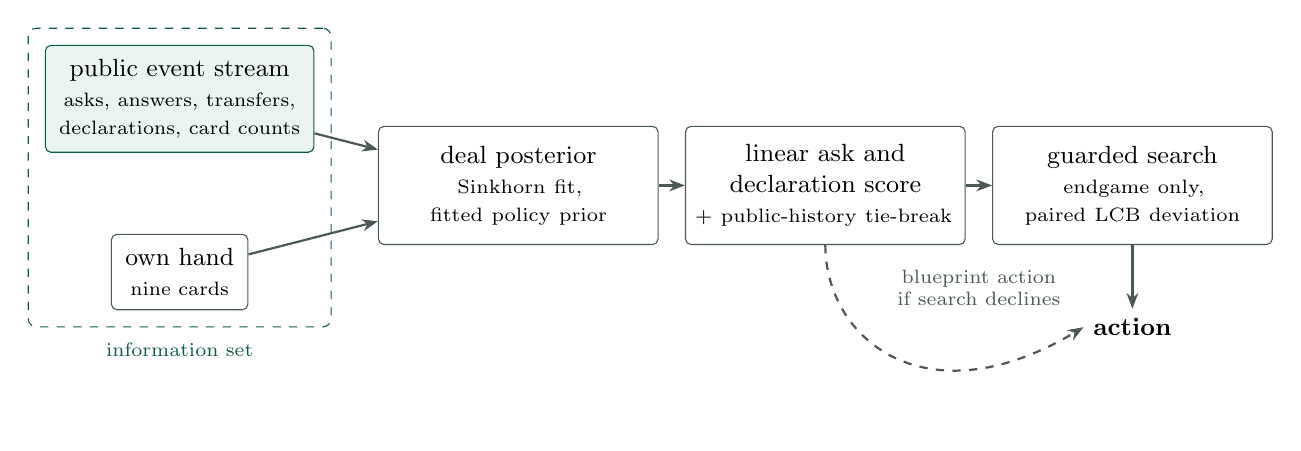
\begin{tikzpicture}[
  font=\small,
  box/.style={draw=fishgray,rounded corners=2pt,align=center,inner sep=5pt,minimum height=9mm},
  % the three pipeline stages carry the same amount of content, so they are
  % held to one height rather than left to differ by the 1pt their last lines do
  stage/.style={box,minimum height=15mm,text width=32mm},
  pub/.style={box,fill=fishlight,draw=fishgreen},
  arr/.style={-{Stealth[length=2mm]},fishgray,thick}]
\node[pub] (hist) at (0,1.15) {public event stream\\{\scriptsize asks, answers, transfers,}\\[-1pt]{\scriptsize declarations, card counts}};
\node[box] (hand) at (0,-1.05) {own hand\\{\scriptsize nine cards}};
\node[stage] (bel)  at (4.3,0.05) {deal posterior\\{\scriptsize Sinkhorn fit,}\\[-1pt]{\scriptsize fitted policy prior}};
\node[stage] (pol)  at (8.2,0.05) {linear ask and\\declaration score\\{\scriptsize + public-history tie-break}};
\node[stage] (srch) at (12.1,0.05) {guarded search\\{\scriptsize endgame only,}\\[-1pt]{\scriptsize paired LCB deviation}};
\node[align=center] (act) at (12.1,-1.75) {\textbf{action}};
\draw[arr] (hist) -- (bel); \draw[arr] (hand) -- (bel);
\draw[arr] (bel) -- (pol); \draw[arr] (pol) -- (srch); \draw[arr] (srch) -- (act);
\draw[arr,dashed] (pol.south) .. controls +(0,-1.2) and +(-2,-1.2) .. (act.west);
\node[font=\scriptsize,fishgray,align=center] at (10.15,-1.25) {blueprint action\\if search declines};
% The enclosure is fitted to the two nodes it contains rather than drawn at
% hand-measured coordinates: at (-1.75,1.75) its sides ran along the borders of
% the public-event-stream box, which is exactly as wide as the rectangle was.
\node[draw=fishgreen,dashed,rounded corners=3pt,inner sep=6pt,fit=(hist)(hand)] (iset) {};
\node[font=\scriptsize,fishgreen,below=2pt of iset] {information set};
\end{tikzpicture}
\caption{The information structure of a Fish seat and the \sestina{} decision pipeline. A seat
observes the public event stream and its own hand, and nothing else; there is no path from a policy to
the deal or to another seat's hand (\S\ref{sec:inference-engine}). Because every card movement is public, that information set
determines an exact posterior over the initial deal (\S\ref{sec:inference}). The deployed path does
not construct it: it runs a cheaper approximate fit that starts from a policy prior and imposes the
same constraints iteratively (\S\ref{sec:inference-prior}). The search runs
only in the endgame and departs from the blueprint's choice only when a paired lower-confidence bound
justifies it (\S\ref{sec:agent-search}).}
\label{fig:pipeline}
\end{figure}

\begin{table}[!ht]\centering
\caption{Components of \sestina{} against \vsix{}. Harness identifiers appear in parentheses and
are used in the paper only where a command must be reproduced.}
\label{tab:components}
{\tabfont\begin{tabularx}{\linewidth}{@{}Q{0.77} Q{0.92} Q{1.31} l@{}}
\toprule
Component & v0.6 & SESTINA v1.0 & Section \\
\midrule
Deal inference & Sinkhorn fit to the deal posterior, from a fitted policy prior & unchanged & \S\ref{sec:inference} \\
Ask and declaration policy & fitted linear score, 37 coordinates & unchanged; no refit in this cycle & \S\ref{sec:agent-policy} \\
Tie-breaking among equal-scoring asks & enumeration order (unstable sort) & hash of the public event stream (\texttt{rtie}) & \S\ref{sec:agent-tiebreak} \\
Half-suit contestation & absent & contested-half-suit weight (\texttt{r12}) & \S\ref{sec:agent-contest} \\
Declaration urgency escalation & event-count clock at 220 events & disabled (\texttt{pool}, \texttt{oppfloor}, \texttt{force}, \texttt{askfloor}) & \S\ref{sec:agent-urgency} \\
Termination safeguard & the urgency clock & deduction-state stall detector (\texttt{stall}) & \S\ref{sec:agent-stall} \\
Test-time search & built and measured, deployed disabled & enabled, endgame-truncated, paired LCB guard & \S\ref{sec:agent-search} \\
\bottomrule
\end{tabularx}}
\end{table}

\subsection{The decision problem, and the ask policy}
\label{sec:agent-policy}

At its turn a seat faces one decision with two branches: declare a half-suit, or ask. Declaration is
treated first in the code and is described in \S\ref{sec:agent-declare}; this subsection covers the
ask.

\paragraph{The legal action set.} With $\mathcal{O}_s$ the opponents and $\mathcal{H}_t$ the
half-suits not yet claimed, the rules of \S\ref{sec:game-rules} give
\begin{equation}
  \mathcal{A}_t \;=\; \bigl\{(c,q) \;:\; q \in \mathcal{O}_s,\; \text{hand}_t(q) \neq \emptyset,\;
  H(c) \in \mathcal{H}_t,\; c \notin \text{hand}_t(s),\;
  \text{hand}_t(s) \cap H(c) \neq \emptyset \bigr\}.
  \label{eq:legal}
\end{equation}
The last condition is what makes every ask informative: the asker must already hold a card of the
half-suit, so asking publishes partial ownership.

What the policy actually enumerates is a strict subset of \eqref{eq:legal}. A \emph{live-ask filter} first removes candidates the seat can already prove are misses, that is,
those whose target is excluded by a certificate, $q \notin \mathcal{M}(c)$. It is this filter, rather
than any weighting inside \eqref{eq:askscore}, that keeps a provably dead ask off the score. It
binds: it removes what would otherwise have been the argmax at roughly \vsevenGateBindRate\% of
\vsevenGateBindN{} ask decisions captured from \sestina{}'s own seats. If no candidate survives the filter the full legal set is
restored, so the guarantee is not absolute.

\paragraph{The score.} Each candidate is scored by a fitted linear function of a
$20$-dimensional feature vector $\phi(a)$, plus a learned value term and, in \sestina{}, three
additional ownership terms:
\begin{equation}
  u(a) \;=\; \lambda\, w^{\!\top}\phi(a) \;+\; \beta\, V_{\mathrm{ask}}(a)
  \;+\; \lambda\bigl(w_{\mathrm{void}}\, g_1(a) + w_{\mathrm{team}}\, g_2(a)
  + w_{\mathrm{last}}\, g_3(a)\bigr),
  \label{eq:askscore}
\end{equation}
with $\lambda = \vsevenLinearWeight{}$ and $\beta$ scale parameters of the fit. \sestina{} adds a
fourth block of \vsevenResponderTotal{} extended coordinates, of which
\vsevenResponderNonzero{} is non-zero; that one is \eqref{eq:contest} and
\S\ref{sec:agent-contest} gives it. Writing $p_a = \hat\mu(c,q)$ for the modelled
hit probability, the features $\phi$ are functions of the belief and the public state. They include $p_a$ and $p_a^2$; an indicator that the card is publicly
certain; the acting seat's holding in $H(c)$ and the posterior mass its team already carries; the
best continuation probability elsewhere in the half-suit; the
reply threat and exposure a miss would create, both weighted by $1-p_a$; the target's hand size and
an indicator that this ask would empty it; the binary entropy $\mathrm{H}_2(p_a)$; and a score-margin
term. Appendix~\ref{app:parameters} lists all twenty with their fitted weights.

The three extra terms are the ones \vsix{} added, and each expresses an effect the twenty could not:
\begin{align}
  g_1(a) &= p_a \prod_{c' \in H(c) \setminus \{c\}} \bigl(1 - \hat\mu(c',q)\bigr),
    \label{eq:gvoid}\\
  g_2(a) &= \Pr\bigl[\,\mathrm{own}(c) \in \mathcal{T}_s \cup \{s\}\,\bigr],
    \label{eq:gteam}\\
  g_3(a) &= p_a \cdot \ind\bigl[\,q \text{ is the last opponent holding cards, and holds one}\,\bigr].
    \label{eq:glast}
\end{align}
Equation~\eqref{eq:gvoid} is the probability that the ask takes the target's \emph{last} card of the
half-suit, \eqref{eq:gteam} the posterior mass the acting team already carries, so a measure of how
wasteful the ask is, and \eqref{eq:glast} an indicator that the ask would trigger the forced
endgame.
Equation~\eqref{eq:gvoid} prices information denial in its bluntest form. Because a legal ask requires
holding a card of the half-suit, removing a target's last card of $H(c)$ permanently removes that
target's right to ask in it.

\paragraph{Selection.} The policy takes the argmax, with the tie handling of
\S\ref{sec:agent-tiebreak} and, when enabled, the search of \S\ref{sec:agent-search}:
\begin{equation}
  a^\star \;=\; \operatorname*{arg\,max}_{a \in \mathcal{A}_t} u(a).
  \label{eq:argmax}
\end{equation}

\sestina{} inherits $w$, $\lambda$, $\beta$ and the three extra weights from \vsix{} unchanged.
\textbf{No gradient or population fit was run in this cycle}: the one coordinate that is not
inherited, \eqref{eq:contest}, had its value chosen as the argmax of a measured dose response, which
is a one-dimensional selection on win rate and is reported as such in
\S\ref{sec:results-selection}. The vector was found by \vsix{}'s repaired
optimiser under a minimax-regret objective over a four-member opponent panel. Of the
\vsevenCoordinates{} coordinates in the extended vector a number are known to be inert, and
Appendix~\ref{app:parameters} lists which and why.

\subsection{Tie-breaking that preserves common knowledge}
\label{sec:agent-tiebreak}

In the \vsix{} mirror, \vsevenTieContested\% of contested ask decisions end with two or more
candidates scoring bit-for-bit identically under \eqref{eq:askscore}
(\S\ref{sec:background-vsix}), and the winner was whichever the enumerator emitted first, under an
unstable sort. That is a correctness problem rather than a strength problem. The choice is arbitrary,
but it is also unpredictable, and \S\ref{sec:game-why} explains why unpredictability of the wrong kind
is expensive here: three identical deterministic teammates coordinate for free only if each can
compute what the others will do, and a tie broken by an implementation detail is not something a
teammate can reconstruct.

Order the candidates by score and let the tied set be
\begin{equation}
  \mathcal{E}_t \;=\; \bigl\{a \in \mathcal{A}_t \;:\; u(a) \ge u(a_{(1)}) - \varepsilon \bigr\},
  \label{eq:tieset}
\end{equation}
where $a_{(1)}$ is the top-ranked candidate and $\varepsilon$ is a fixed tolerance. \sestina{}
replaces enumeration order with a deterministic draw keyed by the public record:
\begin{equation}
  a^\star \;=\; \mathcal{E}_t\bigl[\,\iota(\rho,\,|\mathcal{E}_t|)\,\bigr],
  \qquad
  \rho \;=\; \mathrm{hash}\bigl(\mathcal{P}_t,\; s,\; t\bigr),
  \label{eq:tiebreak}
\end{equation}
with $\mathcal{P}_t$ the running hash of the public event stream, $s$ the seat index, $t$ the event
count, and $\iota$ an index map from the hash into the tied set. Every seat observes all three arguments, so every teammate can recompute $\rho$; no seat's private
hand enters it, and the choice is reproducible from the public record rather than being an artefact
of the enumerator's sort order.

Two scope conditions belong with that. \eqref{eq:tiebreak} governs the non-search path only: when
the endgame search fires it supplies its own selection (\S\ref{sec:agent-search}) and index $0$ is
whatever the sort left first. And the search draws its determinizations from a private per-seat
stream seeded from the harness, so the policy is a deterministic function of
$(\text{own hand}, \text{public record}, \text{reset seed})$ rather than of the first two alone. That
third argument is exactly what the side-channel audit of \S\ref{sec:evaluation-side} replays, which
is why the audit is a test of seat isolation and not of determinism.

The engine also offers a variant that draws $\rho$ from a private per-seat stream. That variant is
\emph{not} used: it would break the reconstructibility that makes \eqref{eq:tiebreak} a coordination
device. \S\ref{sec:development-tie} reports what happened when a later experiment tried to
\emph{select} within $\mathcal{E}_t$ rather than randomise over it.

\subsection{Half-suit contestation}
\label{sec:agent-contest}

The one component carrying measurable strength is a single additional coordinate, one non-zero entry
out of \vsevenResponderTotal{} in an extended block of the parameter vector. Let $M_H$ be the expected number of cards of half-suit $H$ held by the
opposing team, and $q_H$ the number whose holder this seat cannot place. The term is
\begin{equation}
  r(a) \;=\; (1 - p_a)\cdot\frac{M_{H(c)}}{6}\cdot\frac{q_{H(c)}}{6},
  \label{eq:contest}
\end{equation}
entering \eqref{eq:askscore} with a \vsevenContestSign{} coefficient of
\texttt{\vsevenContestWeight{}}, so a large value \emph{encourages} the ask. It selects asks that are
likely to miss, into half-suits the opponents dominate, whose ownership is still ambiguous.

\paragraph{The mechanism is not the one the coordinate was written for, and saying so matters.} The
feature was designed to price \emph{information denial}: a failed ask publishes a negative
certificate, and the intent was that the fitted coefficient would come out negative, meaning refuse
to hand that certificate over. It came out positive. The negative branch was swept separately and is
flat to negative throughout, reaching \vsevenContestNegDose{}~pp at the mirror-image dose, so the design intent is
\textbf{refuted rather than merely unexplored}.

What the positive branch does was measured on the target rather than inferred. Over $\sim$\vsevenContestDecisions{}
target ask decisions, the target's ask accuracy falls from \vsevenContestTargetAskBefore{} to
\vsevenContestTargetAskAfter{}, while its declaration
accuracy \emph{rises} and it becomes \emph{less} often urgent, which rules out the declaration
channel where this phase expected to find everything. The reading the artifact supports is
contestation: asking into half-suits the opponents are trying to complete degrades the quality of
their asks, and the acting team pays part of the same cost, its own ask accuracy falling from
\vsevenContestSelfAskBefore{} to \vsevenContestSelfAskAfter{}. Three sibling coordinates written to express the same denial idea were measured
at the same dose and are inert or harmful, which is what pins the effect to this combination rather
than to opponent mass in general.

Two facts about its provenance matter for \S\ref{sec:results-attribution}. It was found by a
coordinate sweep during adversary generation rather than by architecture work, and it is hand-set:
the value \texttt{\vsevenContestWeight{}} is the argmax of a dose response measured at
\vsevenPhaseTwoCell{} games a dose, not the output of a gradient or population fit. And it is not
uniformly good. Against the then-deployed policy it scored \vsevenOneSwitchArm{}~pp, but its worst
cell over the \vsix{} frontier is \vsevenOneSwitchArmWorst{}~pp against
\texttt{\vsevenOneSwitchArmWorstOpp{}}, which is negative, so it is a strength gain with a worst case
rather than an exploit (\S\ref{sec:development-adversaries}).

\subsection{The declaration rule}
\label{sec:agent-declare}

A declaration names, for each of the six cards of a half-suit, which member of the declaring team
holds it. It is all-or-nothing: correct, and the team scores the half-suit; wrong, and the opponents
do. The decision therefore has two parts, choosing what to claim and choosing when.

\paragraph{What to claim.} For half-suit $h$ the agent takes the most probable allocation among its
own team,
\begin{equation}
  \alpha^\star(h) \;=\; \operatorname*{arg\,max}_{\alpha:\,H \to \mathcal{T}_s \cup \{s\}}
  \; \pi_{\mathrm{alloc}}(h,\alpha),
  \label{eq:bestalloc}
\end{equation}
with $\pi_{\mathrm{alloc}}$ from \eqref{eq:alloc}. \eqref{eq:bestalloc} is the object; it is not what the deployed path computes.
\sestina{} enumerates the capacity-feasible assignments of the unresolved cards of $h$ to its own
team and takes the argmax of the \emph{product of per-card marginals},
$\prod_{c} \hat\mu(c,\alpha(c))$. That product is the selection score only. The winner is then priced
separately, by sequential conditioning: the belief is refit after each card of the allocation is
fixed in turn, and the resulting chain-rule product is what the policy reports as
$\pi^\star_{\mathrm{alloc}}$ and thresholds on. The exact
object \eqref{eq:alloc} is available from the block dynamic program but sits on no decision path. \S\ref{sec:development-alloc} reports the
measurement that closed the question of whether that shortcut costs anything: over
$\sim$\vsevenLoneDecls{} recorded declarations it selects the same allocation as the \emph{sequential joint's} argmax every time, because that
joint's first chain-rule factor \emph{is} the marginal and
the renormalisation that follows reweights the survivors without reordering them.

\paragraph{When to claim.} Write $\pi_{\mathrm{alloc}}^\star = \pi_{\mathrm{alloc}}(h,\alpha^\star)$
and $\pi_{\mathrm{team}}$ for the probability the team owns $h$ outright. The value function is written on the assumption that waiting is free, on the ground that an opponent
cannot claim a half-suit the acting team provably holds. That ground binds strictly only in the
locked case, and the rule is applied down to a team-ownership probability well below one, so the
assumption is an approximation rather than an identity. Under it the decision is not a race but a
trade: declaring scores a point now with probability $\pi_{\mathrm{alloc}}^\star$, and
publishes the team's holdings either way. The agent evaluates that with its learned state-value
function $V$:
\begin{equation}
  \Delta \;=\; \underbrace{\pi_{\mathrm{alloc}}^\star\, V(\text{state} \mid \text{correct})
  \;+\; (1-\pi_{\mathrm{alloc}}^\star)\, V(\text{state} \mid \text{wrong})}_{\text{declare}}
  \;-\; \underbrace{V(\text{state})}_{\text{wait}},
  \label{eq:declev}
\end{equation}
and declares when $\Delta > \delta$ for a fitted margin $\delta$. Both conditioned states differ from the waiting state in having the \emph{unresolved} cards of $h$
removed from the unresolved set, typically fewer than six, and in the deltas of the four
half-suit-control features the value function reads, all of which are functions of the team's
expected share of $h$ before the claim. They differ from \emph{each other} only in the score margin,
by $+1$ and $-1$.

Two overrides sit above \eqref{eq:declev}. Under the forced endgame, when the opposing team is
cardless and the acting team must resolve the remaining half-suits among itself, the agent declares
on a threshold, $\pi_{\mathrm{alloc}}^\star \ge \tau$, and on a lower threshold once $\pi_{\mathrm{team}} > 1 - 5\times10^{-4}$, since a half-suit the team certainly owns will have to be
claimed eventually and delay only costs information. Under \emph{pressure}, the escalation described next, stage 1 lowers the thresholds and stage 2
removes them: the best available allocation is declared unconditionally, whatever its probability.
\sestina{} removes the mechanism that used to raise pressure in ordinary play, and
\S\ref{sec:agent-stall} is what now supplies stage 2.

\subsection{Removing the urgency escalation}
\label{sec:agent-urgency}

\vsix{} inherited a declaration-urgency escalation keyed to an event counter. Past a threshold of 220
public events the declaration rule lowers its team-ownership floor and begins cashing half-suits at
close to a coin flip, which costs \vsevenCliff{}~pp to a policy held in that regime. No adversary
reaches it, since the longest game any adversarial search produced against an unmodified opponent is
\vsevenCliffIncumbentTail{} events, but the machinery is defective in ordinary play as well:
\S\ref{sec:development-alloc} reports that removing it eliminates \vsevenLoneUrgencyShare\% of the
entire declaration allocation-error class. \sestina{} disables it
(\texttt{pool}, \texttt{oppfloor}, \texttt{force}, \texttt{askfloor}).

The escalation was, however, also the policy's termination safeguard, so removing it creates an
obligation.

\subsection{A stall detector as the replacement termination safeguard}
\label{sec:agent-stall}

The escalation \sestina{} removes was keyed to a clock. The condition the clock stood in for is
``nothing is happening any more'', and that condition is directly observable from the seat's own
deduction state, which is both tighter and safer.

Let $\chi_t = \mathrm{hash}\bigl(\mathrm{own}_t(\cdot),\, \mathcal{M}_t(\cdot),\, U_t,\,
(\text{hand sizes})_t,\, (\text{live half-suits})_t\bigr)$, the digest of the hard certificates the
seat holds. It deliberately \emph{excludes} the list of outstanding (C5) disjunctions: a repeated ask
appends a duplicate disjunction carrying no information, so counting that list as progress would
blind the detector to the one loop it exists to break. Define the
no-progress counter
\begin{equation}
  \nu_t \;=\;
  \begin{cases}
    0, & \chi_t \neq \chi_{t-1},\\
    \nu_{t-1} + 1, & \chi_t = \chi_{t-1},
  \end{cases}
  \label{eq:stall}
\end{equation}
and escalate to pressure stage 1 when $\nu_t \ge K$ and to stage 2 when $\nu_t \ge 2K$, with
$K = \texttt{\vsevenOptStallK{}}$ and $2K = \texttt{\vsevenOptStallTwo{}}$ in \sestina{}.

\paragraph{Why it is a safeguard and not a guarantee.} Consider
$\Phi_t = \sum_{c \in U_t}\bigl(|\mathcal{M}_t(c)| - 1\bigr) + |U_t| + |\mathcal{H}_t|$. Certificates
only accumulate: a seat excluded from a card's candidate set is never restored, a resolved card is
never unresolved again, and a claimed half-suit never returns. Every event that changes $\chi$ by one
of those routes therefore strictly decreases $\Phi_t$, which is a non-negative integer, so there can be
only finitely many of them. \textbf{This argument does not close.} The digest also contains hand
sizes, so a successful ask always counts as progress, and a card moving between two seats is not a
monotone gain; nothing above forbids a card being won back later. The rule therefore bounds the mode
of non-termination that actually occurs, a run of asks producing no new certificate, and not every
mode. That is why this paper calls it a safeguard, and why \S\ref{sec:discussion-engineering} records
termination as empirical.

The threshold was set from measurement. Over \vsevenStallMirrorGames{} mirror games \vsix{} never
produces a no-progress run longer than \vsevenStallIncumbentRun{}, while the deliberately deadlocked
negative control of \S\ref{sec:evaluation-gate} produces \vsevenStallFrozenRun{}. Any
$K \in [12,60]$ is therefore simultaneously unreachable in ordinary play and immediate in a deadlock.
Armed, the rule's mirror transcript digest is byte identical to the same configuration without it:
its cost in ordinary play is not small but identically zero, because $\nu_t$ never reaches $K$.
\S\ref{sec:results-attribution} confirms that on holdout material. Note also that $\nu_t$ is a
function of the seat's own hand and the public record alone, so the rule opens no information
channel.

\subsection{Guarded determinized test-time search}
\label{sec:agent-search}

\sestina{} enables the search \vsix{} built, measured, and then deployed switched off. It runs only
in the endgame, when at most \texttt{\vsevenOptMaxq{}} cards remain unresolved, and it revises the
blueprint's choice only when a paired statistical test says it should.

\paragraph{Sampling worlds.} The search draws $D_{\mathrm{det}} = \texttt{\vsevenOptDet{}}$
determinizations from the exact posterior of \eqref{eq:posterior}, using a per-card capacity dynamic program as a uniform sampler over deals
satisfying (C1)--(C4), with the (C5) disjunctions enforced by rejection, so an accepted draw is an
exact sample. This sampler is a distinct object from the block program of \S\ref{sec:inference-factor},
which enumerates (C5) inside its blocks instead. $D_{\mathrm{det}}$ is a target rather than a
guarantee: draws are attempted up to a cap and the rule proceeds with however many survive
rejection. The policy prior of \eqref{eq:prior} is then applied as an
importance weight rather than baked into the sampler, which keeps the sampler exact and the prior
auditable:
\begin{equation}
  \tilde w_d \;=\; \prod_{c \in U_t} \exp\Bigl(\operatorname{clip}\bigl(\theta\, a_{o_d(c),H(c)}
  - \varphi\,(A_{o_d(c)} - a_{o_d(c),H(c)}),\, \pm 2.6\bigr)\Bigr),
  \qquad
  w_d = \frac{\tilde w_d}{\sum_{d'} \tilde w_{d'}},
  \label{eq:iw}
\end{equation}
where $o_d(c)$ is the seat holding card $c$ in world $d$.

\paragraph{Rolling out.} The candidate set is the top $\texttt{\vsevenOptCand{}}$ blueprint
candidates, with index $0$ reserved for the blueprint's own choice $a_{(1)}$. For each candidate $r$ and world $d$, all six seats are reconstructed \emph{at their own information
sets} under $d$, each playing a cheaper blueprint than the acting agent's own: the \vfive{} policy
with an independent-marginal belief and no re-scoring pass and the game is played to a terminal state or until \texttt{\vsevenOptDepth{}} further public events
have elapsed. A run reaching the end returns the acting team's half-suit differential; a run cut at the limit
returns a \emph{material} evaluation of the position instead, being the scored half-suit differential
plus the team's expected control of the live half-suits. That is \vsix{}'s own hand-written leaf, not
a learned one: \S\ref{sec:development-leaf} reports what happened when a fitted replacement was
built. Write $V_{r,d}$ for either. This is the point at which the method departs from standard
determinization: the continuation players are not made clairvoyant. \S\ref{sec:game-why} explains why
that matters here, namely that clairvoyant play in Fish is degenerate and every action would score
alike. All candidates share the same $D_{\mathrm{det}}$ worlds, so the comparison is paired and the
noise that matters is the noise in the difference.

\paragraph{The guarded deviation rule.} For each candidate $r \ge 1$ form the paired difference
against the blueprint,
\begin{equation}
  m_r \;=\; \sum_{d} w_d\,\bigl(V_{r,d} - V_{0,d}\bigr),
  \qquad
  \mathrm{var}_r \;=\; \sum_{d} w_d\,\bigl(V_{r,d} - V_{0,d} - m_r\bigr)^2,
  \label{eq:paired}
\end{equation}
and with the Kish effective sample size $n_{\mathrm{eff}} = 1/\sum_d w_d^2$ take
\begin{equation}
  \mathrm{se}_r = \sqrt{\frac{\mathrm{var}_r}{n_{\mathrm{eff}} - 1}},
  \qquad
  \mathrm{LCB}_r = m_r - \kappa_r\,\mathrm{se}_r + \eta\,\bigl(u(a_{(r+1)}) - u(a_{(1)})\bigr).
  \label{eq:lcb}
\end{equation}
The search deviates to $\arg\max_r \mathrm{LCB}_r$ if that maximum is positive, and otherwise plays
the blueprint's choice. The shrinkage is $\kappa = \texttt{\vsevenOptKappa{}}$. The term $\eta$ blends the blueprint's own
ranking back in and is \textbf{zero in this configuration}, so \eqref{eq:lcb} reduces to a pure
paired lower confidence bound.

Equation~\eqref{eq:lcb} is the whole of what makes the machinery usable. Chosen instead by an
unguarded $\arg\max_r m_r$, the same search is \vsixCurseGap{}~pp \emph{worse} than the blueprint it
searches from (\S\ref{sec:background-vsix}): one world's return is a final half-suit differential
whose spread is an order of magnitude larger than genuine differences between candidates, so the
maximum selects on residual noise, and does so more confidently the more candidates it is offered.
Requiring $\kappa$ standard errors of a \emph{paired} difference removes that.

One detail is worth stating because \S\ref{sec:development-tie} turns on it. Within the tied set
$\mathcal{E}_t$ of \eqref{eq:tieset} the rule applies $\kappa_r = 0$, that is, no shrinkage at all,
which is precisely where its selection signal is most noise-dominated.

\subsection{How three teammates coordinate without communicating}
\label{sec:agent-coordination}

\sestina{} deploys as three identical agents. They hold different private hands, they may not
signal, and the only channels the dialect leaves are the forced-endgame willingness bit and the
successor a cardless turn-holder names (\S\ref{sec:game-dialect}), both of which
\S\ref{sec:game-dialect} measures as empty or near-empty. So all coordination has to come from
somewhere else.

It comes from determinism plus a shared observation. Let $\Pi$ denote the policy, a map from
$(\text{own hand}, \text{public record})$ to an action. Every teammate runs the same $\Pi$ and
observes the same public record $\mathcal{P}_t$. Teammate $j$ cannot compute $\Pi$'s output at seat
$i$, because it does not know $i$'s hand. But it knows $\Pi$ itself, and it knows $\mathcal{P}_t$, so
it can compute the \emph{distribution} of $i$'s action induced by its own posterior over $i$'s hand,
\begin{equation}
  \Pr\bigl[\,a_i = a \mid \mathcal{I}_j^t\,\bigr]
  \;=\; \sum_{D \,\models\, \mathcal{I}_j^t}
  \Pr\bigl[D \mid \mathcal{I}_j^t\bigr]\;
  \ind\!\left[\Pi\bigl(\text{hand}_i(D),\, \mathcal{P}_t\bigr) = a\right],
  \label{eq:coord}
\end{equation}
and, having observed $a_i$, condition on it. That is exactly the (C5) reasoning of
\S\ref{sec:inference-constraints} carried one step further: a legality certificate says the asker
held \emph{some} card of the half-suit, while \eqref{eq:coord} says the asker held a hand on which
$\Pi$ preferred that ask. The deployed approximation does not evaluate \eqref{eq:coord} in full,
which would require enumerating hands; it captures the first-order part of it through the ask-tally
prior \eqref{eq:prior}. The white-box adversary of \S\ref{sec:results-whitebox} is the construction
that evaluates \eqref{eq:coord} against \sestina{} rather than for it, and
\S\ref{sec:development-instrument} reports what that inversion is worth.

Two conditions make this work, and both are engineering constraints rather than assumptions. $\Pi$
must be \emph{reconstructible}: a teammate reasoning about seat $i$ must be able to evaluate
$\Pi(\cdot,\mathcal{P}_t)$ on a hypothesised hand. An unstable sort does not break determinism, since
it is deterministic for a fixed input and build, but it does break reconstructibility, because the
result depends on an implementation detail no teammate can model. \eqref{eq:tiebreak} restores it on
the non-search path. And $\Pi$ must be common
knowledge, which for three copies of one published agent it is. No shared secret and no pre-play
randomisation are needed or used, which is the sense in which the team's correlation device is public
(\S\ref{sec:threat}).

\paragraph{One defect the evaluation runs under.} Agents are constructed once per worker thread and
reused across the deals that thread is given, and some per-agent state survives the inter-deal reset,
reachable only under the search. This violates the premise that $\Pi$ depends on
$(\text{own hand}, \mathcal{P}_t)$ alone: a decision can depend on which deals the thread happened to
process earlier. The carrier was identified as the rollout engine, which the reset never touches; the
specific field was not. It was deliberately not repaired, because the one-line fix changes the play of
every searching configuration by roughly one deal in \vsevenSsixIncidence{}, and applying it after the
configuration was frozen would defeat the purpose of freezing.
\S\ref{sec:results-controls} measures its magnitude on holdout material, and
\S\ref{sec:discussion-engineering} states what it costs the argument above.

\subsection{The complete decision procedure}
\label{sec:agent-full}

Collecting the pieces, one turn of \sestina{} at seat $s$ and time $t$ runs as follows.

\begin{enumerate}
\item \textbf{Update beliefs.} Fold the new public events into the candidate sets
  $\mathcal{M}_t(\cdot)$ by (C1)--(C5), then compute $\hat\mu$ by \eqref{eq:prior} and
  \eqref{eq:sinkhorn}. Update the no-progress counter $\nu_t$ by \eqref{eq:stall}.
\item \textbf{Consider declaring.} For each live half-suit form $\alpha^\star$ by
  \eqref{eq:bestalloc} and its probability $\pi_{\mathrm{alloc}}^\star$ by \eqref{eq:alloc}. Declare
  if $\Delta > \delta$ in \eqref{eq:declev}, or if a pressure or forced-endgame override fires
  (\S\ref{sec:agent-declare}).
\item \textbf{Otherwise ask.} Enumerate $\mathcal{A}_t$ by \eqref{eq:legal} and score every candidate
  by \eqref{eq:askscore}, including the contestation term \eqref{eq:contest}.
\item \textbf{Resolve ties.} Form $\mathcal{E}_t$ by \eqref{eq:tieset}. If the endgame condition does
  not hold, return \eqref{eq:tiebreak} and stop.
\item \textbf{Search.} Otherwise sample $D_{\mathrm{det}}$ worlds with weights \eqref{eq:iw}, roll out
  each candidate in each world, and return the candidate selected by \eqref{eq:lcb}, which is the
  blueprint's own choice unless a candidate clears it by $\kappa$ standard errors.
\end{enumerate}

Every step reads only the acting seat's own hand, the public record and, in step 5, its own reset
seed. That is what makes the coordination argument of \S\ref{sec:agent-coordination} go through, and it is the property the
side-channel audit of \S\ref{sec:evaluation-side} tests mechanically rather than by inspection.

%% --- end sections_v07/06-agent ---
%% --- begin sections_v07/07-evaluation ---
\section{Evaluation framework}
\label{sec:evaluation}

Roughly half of what this project has produced is its evaluation method, and it is presented here as
method rather than as process, because each component was adopted in response to a specific measured
failure and each is portable to another game. \S\ref{sec:background-vsix} describes the failures.

\subsection{The outcome measure}
\label{sec:evaluation-measure}

The primary outcome is the team win rate, the proportion of games in which the evaluated
configuration's team takes at least five of the nine half-suits. Comparisons are reported as an
\textbf{edge in percentage points},
\[
  \text{edge} \;=\; 100 \times (\text{win rate} - 0.5),
\]
so that zero denotes indistinguishable configurations and the sign gives the direction. The paper
writes \emph{pp} for percentage points of this quantity. Three other quantities appear and are never
conflated with it: the mean number of half-suits a team takes, used for the search's internal return;
predictive log loss and argmax hit rate, used to score posteriors as predictors
(\S\ref{sec:background-vsix}); and the adversarial edge of \S\ref{sec:results-adversarial}, which is
an edge in the same units but measured for a fitted opponent against the evaluated configuration.

\subsection{Duplicate deal blocks}
\label{sec:evaluation-duplicate}

A \emph{cell} compares two configurations $A$ and $B$ over a \emph{bank} of deals identified by one
integer seed. Every deal in the bank is played twice: once with $A$ in the odd seats and $B$ in the
even seats, and once with the seats exchanged. Both configurations therefore play the identical deal
from both sides.

Fish has large per-deal variance, since a deal can be won or lost on the cards, and an unpaired
comparison spends most of its sample resolving that variance rather than the difference between
policies. The rotation cancels the deal's intrinsic advantage exactly, in the spirit of duplicate
bridge and of the variance-reduction estimators developed for poker
\cite{zinkevich-divat,burch-aivat}. The design requires reproducibility from the seed alone
(\S\ref{sec:inference-engine}); without it the two rotations are not the same deal and the design
degrades silently into an unpaired one.

\subsection{Deal-clustered bootstrap confidence intervals}
\label{sec:evaluation-intervals}

The two rotations of one deal are not independent observations. They share a deal and their outcomes
are negatively correlated by construction, so treating them as independent understates uncertainty.

Every interval in this paper is a two-sided 95\% \textbf{deal-clustered bootstrap confidence
interval}. The resampling unit is the \emph{deal}, carrying both of its rotations together; 20{,}000
bootstrap resamples are drawn with replacement from the deals of the cell, the edge is recomputed on
each resample, and the interval is the empirical 2.5th and 97.5th percentiles of that distribution.
No Wilson or normal-approximation interval on the game count is quoted anywhere in this paper, and
the substitution is not cosmetic: at these sample sizes it is the difference between a claim that
replicates and one that does not.

Two derived quantities are used throughout and are defined once here.

\paragraph{Pooling two banks.} Two banks of equal size pool as the mean of their two edges, with standard
  error $\mathrm{se}_{\text{pooled}} = \sqrt{\mathrm{se}_1^2 + \mathrm{se}_2^2}/2$, where each
  $\mathrm{se}$ is recovered from that bank's clustered interval as half-width divided by $1.96$. The
  pooled interval is the estimate plus or minus $1.96\,\mathrm{se}_{\text{pooled}}$. Both per-bank
  values are printed beside every pooled figure in this paper.
\paragraph{Differences between separately measured cells.} A difference between two pooled cells, such as
  an ablation's leave-one-out drop, is the difference of the estimates with the two pooled half-widths
  combined in quadrature. This is conservative. The configurations are paired on deals, so a genuine
  paired difference would be narrower, but the harness produces no paired difference \emph{across} two
  separately executed cells, and constructing one would assert more than the data structure supports.

\subsection{Power computed before a cell is run}
\label{sec:evaluation-power}

At parity a cell's 95\% half-width in percentage points is approximately $98/\sqrt{N}$ for $N$ games.
The harness computes this for every cell and emits it with the result. The arithmetic is applied in
advance because it determines what may be attempted: resolving one point requires roughly
\vsevenScoreboardGames{} games, and a quarter of a point requires sixteen times that.

The failure this prevents is the one \S\ref{sec:background-vsix} describes, in which five mechanisms
cleared a 95\% paired interval at one budget and returned exactly zero at three times it. Sample
sizes in this paper are chosen from the arithmetic before a cell is run, never after seeing its
result.

\subsection{Replication across disjoint banks as an advance-specified criterion}
\label{sec:evaluation-replication}

Every claim is measured on two disjoint deal banks, and the criterion was fixed before the data were
seen:

\begin{quote}
A claim whose \textbf{sign} does not agree on both banks is reported as not replicated, whatever its
pooled interval says.
\end{quote}

This is stricter than a pooled significance test, deliberately. A pooled interval can exclude zero
while the two banks disagree, and that configuration has occurred in this corpus and has previously
been published as a positive result. The criterion binds against this paper's own findings in
\S\ref{sec:results-attribution} and again in \S\ref{sec:results-panel}, and both instances are
reported.

\subsection{Sealed material and advance registration}
\label{sec:evaluation-seal}

A programme that generates candidate configurations, scores them and selects the best is performing a
maximisation, and the selected configuration's score is upward biased by the amount a maximum over
$K$ draws exceeds the mean. No care taken in the final measurement removes that bias if the final
measurement uses material the selection has seen.

Before any candidate existed, deal banks were reserved by seed and their digests committed, a digest
being a rolling hash over the six dealt hands and the dealer of every deal in the bank, computed
without constructing a policy or playing a game. An adversary population was split in half by a rule
fixed in advance, and one half was encrypted with the plaintext's SHA-256 committed, so that it could
not be trained against even accidentally. The engine enforces the seal: a run naming a sealed seed
fails unless an explicit environment variable is set, which was set once, at the start of the final
evaluation, and recorded.

The entire final battery, comprising every cell, its sample size, its threshold, the arithmetic
behind the sample size and the conditions that would count as non-confirmation, was written down and
committed before any holdout bank had been played and before the sealed half had been decoded. The
evaluation was then executed from a cleared context, reading that document and nothing else from the
project's records. Where it required a training figure for comparison it took it from the registered
protocol, which states such expectations in advance for exactly this purpose, so that agreement
constitutes a check and disagreement constitutes a finding.

Anything the evaluation did that the protocol does not specify is recorded as a deviation, next to
the affected result. There are \vsevenDeviations{}, listed in Appendix~\ref{app:deviations}.

\subsection{Selection effects and multiple comparisons}
\label{sec:evaluation-multiplicity}

This study evaluates many candidate mechanisms, opponents, ablations, adversarial searches and
configurations, and the inferential status of that needs stating precisely.

\textbf{No formal family-wise or false-discovery correction was applied}, and no interval reported
here is adjusted for multiplicity. What the design provides instead is structural.
\emph{Registration} fixes the primary comparison, its threshold and its interpretation before the
data exist, so the primary claim is a single pre-specified test rather than the best of many.
\emph{Sealing} makes the holdout material unavailable to the selection process by construction rather
than by discipline. \emph{Disjoint banks with a sign criterion} require a claim to appear twice
before it is reported. \emph{Calibration} of the detection floor (\S\ref{sec:evaluation-floor})
establishes what the instrument can resolve, so that a null is interpretable. And an explicit
\emph{selection check} (\S\ref{sec:results-selection}) computes how much of the measured gain a
maximum over $K$ candidates would produce under the null and compares advance-stated training figures
against their holdout counterparts.

Exploratory comparisons in \S\ref{sec:development} are reported as exploratory: they were run on
training material during the development phase, none is treated as confirmatory, and none is used to
support the paper's primary claim.

\subsection{A soundness gate applied before any strength measurement}
\label{sec:evaluation-gate}

Win rate and soundness are dissociable in this policy family. The corpus contains a configuration
that scores \vsevenScoreboardTrapWin\% against an earlier version while making
\vsevenScoreboardTrapDead\% provably dead asks, asks whose target it can already prove does not
hold the card (\S\ref{sec:agent-policy}), and losing \vsevenScoreboardTrapLimit\% of its games to the action cap. It is both stronger and
broken.

A configuration is therefore gated \emph{before} any strength number is computed for it, on \vsevenGateRulesWord{}
rules covering dead asks, dead runs, action-limit games, the mirror game-length tail, late
declarations, and the side-channel tests below. A configuration that fails is rejected regardless of
its win rate. The gate runs on \emph{training} material by design, being a soundness check on
self-play behaviour rather than a strength claim. It is accompanied by a negative control, a
configuration constructed to be rejected, because a gate that cannot reject it would certify nothing
about the configuration it accepts.

\subsection{Calibrated detection floors}
\label{sec:evaluation-floor}

An exploitability figure is produced by a search, and a search that finds nothing admits two
explanations: there is nothing to find, or the search is too weak. A \textbf{detection floor}
separates them. An artificial handicap of known size is planted in a target, a responder is fitted
against the handicapped target, and the \emph{excess} of that responder's edge over its edge against
the unhandicapped target is measured. The smallest planted edge the procedure recovers is the floor.

Two findings from that calibration shape every exploitability statement in this paper. First, the
floor does not decrease with evaluation games. An early prediction that it would fall as
(evaluation games)$^{-1/2}$ was refuted at its own predicted value: at four times the games the floor
is \vsevenPrimaryFloor{}~pp, and the sub-floor rung remains undetected not because the interval is
wide but because the measured excess resolves \emph{to} zero. Below roughly a point and a half a
fitted responder is empty rather than merely unresolved, so the binding constraint is search power
rather than evaluation power. Second, floors are family-specific: the declaration channel has its own
and higher floor of \vsevenDeclFloor{}~pp, and reading a declaration-objective result against the
general floor would overstate it.

An adversary class contributes to an exploitability statement only after passing a planted-edge
calibration at or below the effect size in question. That precondition is why the negative controls of
\S\ref{sec:results-controls} are run: an instrument that cannot recover a planted edge of a given size
cannot report the absence of a real one of that size.

\subsection{Mechanical homogeneity and side-channel controls}
\label{sec:evaluation-side}

The evaluated team is three identical agents with no shared secret. That their coordination is common
knowledge is legitimate (\S\ref{sec:game-why}), but it also means an implementation detail could
become an unintended signalling channel. Before this cycle the constraint had only ever been checked
by reading the source.

Four mechanical tests now run over all four engine decision types. \textbf{S3, listening
substitution} asks whether a seat's behaviour changes more when a teammate's hidden action changes
than when an opponent's does, beyond what the rules explain. \textbf{S4, stream independence} asks
whether the seat's private random stream is drawn independently of the deal. \textbf{S5, posterior
invariance} asks whether the seat's action depends on true card locations beyond what its own
posterior supports. \textbf{S6, seat isolation} replays every decision from own hand, public event
stream, rules and reset seed alone, and counts the decisions the reconstruction cannot reproduce, at
zero tolerance.

The tests are calibrated by three positive controls, each a policy carrying one planted violation,
and each must fail exactly the tests the protocol names for it in advance and no others.
\S\ref{sec:design-material} reports the calibration on holdout material. Without those controls a
clean report from the gate would be uninformative.

One limitation is stated wherever the gate is used. The zero-tolerance form of S6 requires a single
worker thread, because the audit depends on the deal-to-thread partition and work stealing does not
fix that partition at higher counts, and it requires agents rebuilt for each deal. Rebuilding agents
per deal \emph{changes play}. The gate therefore certifies that with cross-deal residue removed,
nothing else depends on anything it should not. The residue itself is not removed from the deployed
mode, and every strength number in this paper is measured under it
(\S\ref{sec:results-controls}).

\subsection{Worst case and minimax regret over a shared panel}
\label{sec:evaluation-panel}

The project's standing reporting rule is that the worst case leads and an aggregate never does, since
a mean over an opponent panel rewards beating weak opponents by larger margins, which is not the
quantity of interest. Two statistics are reported over a panel scored identically for every
configuration: the \textbf{worst cell}, being the panel member on which a configuration does least
well, and the \textbf{minimax regret}, being for each member the shortfall from the best configuration
on that member, maximised over members. They can disagree, and in \S\ref{sec:results-panel} they do.
Reporting both, and reporting the panel mean last and labelled as a diagnostic, is the discipline.

Every configuration must carry a cell for every member or minimax regret is undefined, which is why
the panel is fixed by name in advance and scored for all configurations on the same banks. One
consequence of that design is recorded where it matters: a configuration that is itself a panel
member meets itself and carries a free zero cell, which can only flatter its worst case, so
\S\ref{sec:results-panel} prints the worst case both with and without self-cells.
%% --- end sections_v07/07-evaluation ---
%% --- begin sections_v07/08-threat-model ---
\section{A threat model for a homogeneous deterministic team}
\label{sec:threat}

Robustness claims are only meaningful against a stated adversary, and the adversary appropriate to
this domain is unusual enough to define explicitly. The definition below was written before any v0.7
measurement was taken, and it constrains how \S\ref{sec:results-adversarial} may be read.

\paragraph{The unit is the team.} What is evaluated is the joint policy $\pi = (\pi_1,\pi_2,\pi_3)$
of three identical agents. The principal adversary controls all three opposing seats. A one-seat
deviation column is reported alongside it on the same deals, because a three-seat upgrade and a
one-seat upgrade are different quantities that this corpus has previously conflated
(\S\ref{sec:results-partners}).

\paragraph{The adversary is white-box, with an explicit exclusion list.} It is given the target's
source, its parameter vector, and unlimited offline access to it. It is not given the deal, the deal
seed, any seat's hand, or the engine's confidence field. The exclusions are the point of the
construction. Because the target team is three identical published deterministic agents, its
coordination is common knowledge, which inverts the assumption in the team-correlation literature
that the correlation device is private \cite{celli-gatti,farina-collusion}. The adversary class built
to exploit that property is the transcript inverter of \S\ref{sec:results-whitebox}.

\paragraph{Homogeneity is exactly two prohibitions.} The team receives no shared secret pre-play seed,
and no seat may use an illegal side channel, defined mechanically by the four tests of
\S\ref{sec:evaluation-side} over all four engine decision types. Everything else a seat-conditioned
policy can do is permitted.

\paragraph{Three correlation regimes, and which one is principal.} The three adversary seats may be
fitted independently, may be three copies of one vector, or may share a pre-play signal secret from
the target team. The first is the \emph{independent} regime, the second the \emph{synchronised}
regime, and the third the \emph{ex-ante correlated} regime; the last is the only one whose result
would bear on the target rather than on the search alone, and even there it remains a lower bound.
It is the registered principal case. The synchronised regime is
retained as the continuity column, because it is what earlier cycles of this corpus measured.
\S\ref{sec:discussion-future} records which of the three this study actually reached.

\paragraph{Every exploitability figure is a lower bound.} Each is reported as at least $x$, with the
adversary class, the number of controlled seats, the correlation regime and the search budget
attached. Computing the true value is intractable even white-box. The consequence is stated once and
observed throughout: \textbf{a search that fails to find an exploit is evidence about the search, not
a property of the target}. The v0.4 record in this corpus contains exactly that reading error, having
reported a null result as a demonstration of robustness, and \S\ref{app:corrections} carries the
correction rather than repeating it.

\paragraph{A class contributes only after calibration.} An adversary class is admitted to an
exploitability statement only once it has passed a planted-edge calibration at or below the effect
size being claimed (\S\ref{sec:evaluation-floor}).

\paragraph{What the definition does not license.} It does not license the claim that a policy passing
every test is unexploitable, and it does not license reading the opponent panel's worst cell as an
exploitability figure. The panel measures robustness across playstyles; the adversary search measures
what a fitted responder achieves. They are different objects and this paper keeps them in different
subsections.
%% --- end sections_v07/08-threat-model ---
%% --- begin sections_v07/09-development ---
\section{Developing \sestina{}}
\label{sec:development}

This section reports the development phases: what the instrument was shown to be capable of
detecting, what an open adversary search found, and which candidate mechanisms were tested and
rejected. All measurements here are on \emph{training} material and are exploratory in the sense of
\S\ref{sec:evaluation-multiplicity}. None supports the paper's primary claim, and every pooled
interval reported in this section has a lower bound below the detection floor of
\vsevenPrimaryFloor{}~pp, so each is a measured effect rather than a confirmed one.

\subsection{The v0.6 frontier, and the choice of comparison target}
\label{sec:development-frontier}

\vsix{} deployed its policy with test-time search disabled, while also having measured that search
working. The configurations available at the end of that cycle therefore form a \emph{frontier}
rather than a point, running from the deployed blueprint to progressively more expensive searching
configurations.

This distinction drove the most consequential methodological choice in the programme. Beating the
deployed policy is the easy comparison, and several unfitted single-switch deviations of it already
do. \textbf{The comparison target was therefore fixed as \fcheap{}}, the cheapest configuration that
is genuinely on the frontier, and \S\ref{sec:design-protocol} records that the choice was registered
in advance. Table~\ref{tab:configs} defines every configuration this paper compares.

\subsection{What the instrument can detect}
\label{sec:development-instrument}

The detection-floor procedure of \S\ref{sec:evaluation-floor} was built and calibrated in this
phase, which measured the floor at \vsevenFloorPhaseOne{}~pp and predicted that it would fall as
(evaluation games)$^{-1/2}$. The phase of \S\ref{sec:development-adversaries} re-measured the same
rung at four times the games and got \vsevenPrimaryFloor{}~pp, refuting the prediction; that is the
first of the two findings \S\ref{sec:evaluation-floor} reports, the second being that floors are
family-specific, with the declaration channel's at \vsevenDeclFloor{}~pp. Two further results shape
later sections.

\paragraph{Transcript inversion contracts the posterior, and is not an attack.} Because the target
team is deterministic and published, an adversary can invert its transcript, asking for each observed
ask which deals would have produced it and contracting the posterior accordingly. Measured, this
contracts the deal posterior by approximately \vsevenBitsPerAsk{} bits per observed ask beyond the
certificates the rules already supply. Converting those bits into play is worth
\vsevenInversionUnfitted{}~pp unfitted against the deployed policy.

It is nonetheless not an exploit. The excess tracks planted-edge size to within
$\pm$\vsevenInversionTrack{}~pp on all eight rungs of the calibration ladder, which is the signature
of a general strength gain rather than an exploitation instrument. And no linear handicap adds more
than \vsevenHandicapBits{} bits per ask, so within this policy family there is no readability
handicap available for a stochastic policy to purchase. A brief that proposed a stochastic policy
conditional on the inverter succeeding was therefore closed on its antecedent.

\paragraph{A cost figure the record had wrong.} The \vsix{} paper priced the searching configuration
at ``three orders of magnitude'' the blueprint, a ratio that mixed an all-threads timing with a
single-thread one. Re-timed here on one basis, it is \vsevenPhaseOneCost$\times$. But that figure
describes the \emph{unrestricted} search, which is not the frontier point anything was measured at,
and phase~3 re-measured the endgame-restricted operating point at approximately
\vsevenCostRecorded$\times$. \S\ref{sec:results-cost} corrects that correction in turn.

\subsection{Open adversary generation against the frontier}
\label{sec:development-adversaries}

The constraint on this phase was that the searches must not share a bias, since fifteen runs of one
search constitute one run. Every exploiter search in the corpus before it had been the same search: a
cross-entropy fit of a linear vector maximising win rate from one seed against one target. This phase
constructed six adversary classes in the synchronised regime, plus one fitted search in the
ex-ante-correlated regime, and measured channel ceilings before fitting anything against them.

\paragraph{The principal finding is negative.}
Nothing constructed exploited the \vsix{} frontier beyond
the detection floor. The best measured exploitability of the deployed policy remains an in-class
figure of \vsevenBestExploit{}~pp $[\vsevenBestExploitLo, \vsevenBestExploitHi]$ over
\vsevenBestExploitN{} games, which is below the class floor of \vsevenPrimaryFloor{}. Seven
independently fitted searches confirmed it and none cleared its class floor.

Every configuration that beat the deployed policy by more than the floor proved on measurement to be
a better policy rather than an exploit: the target's own test-time search at
\vsevenSearchAsExploit{}~pp, and a single out-of-class coordinate at \vsevenOneSwitchArm{}~pp whose
gain survives against opponents sharing none of the target's machinery. The second of those is the
contestation weight of \S\ref{sec:agent-contest}; \S\ref{sec:results-attribution} measures on
holdout what it contributes and finds it the largest of the five components \sestina{} carries,
rather than the whole of the gain.

Two further results from this phase bear on \sestina{}'s design. The declaration-urgency channel
that the phase expected to be its headline has a measured ceiling of \vsevenUrgencyCeiling{}~pp
$[\vsevenUrgencyCeilingLo, \vsevenUrgencyCeilingHi]$ and is dead as an attack, but the same channel is
worth \vsevenUrgencyWorthLo{} to \vsevenUrgencyWorthHi{}~pp to a configuration that simply disables
it: the adversary owns the smaller half of a two-point defect in the target. And the event-count
cliff of \S\ref{sec:agent-urgency} is unreachable by any adversary, while a configuration that removes
the counter inherits a self-play game-length tail of \vsevenCliffTail{} events, which is the
obligation \S\ref{sec:agent-stall} discharges.

\subsection{Candidate mechanisms that were tested and rejected}
\label{sec:development-rejected}

Five candidate mechanisms were developed in isolated branches, gated before being scored, and checked against the side-channel definition by the
harness of \S\ref{sec:evaluation-side} rather
than by inspection. \textbf{One survived}, and it is the configuration change described in
\S\ref{sec:agent} rather than an architecture. The four that were rejected are reported here, each
with the measurement that rejected it, because each closes a standing hypothesis in the project's
design register and because a closed direction does not depreciate.

\subsubsection{The declaration-allocation channel is worth zero}
\label{sec:development-alloc}

The design register's second-ranked hypothesis, at priority \vsevenLonePriority{}, held that
\vsix{}'s entire margin lives in the declaration channel and that roughly two points of it remained.
Its proposed mechanism was that the deployed allocator, a product of per-card marginals, selects a
different allocation from the joint posterior's argmax often enough to matter.

It does not. Over approximately \vsevenLoneDecls{} recorded voluntary declarations, across two banks
and both urgency settings, the joint argmax and the marginal-product argmax select the same allocation
at every one, with the joint score holding a strict opinion on
\vsevenLoneStrictLo\% to \vsevenLoneStrictHi\% of genuinely ambiguous cases. The reason is algebraic
rather than statistical: the sequential joint's first chain-rule factor \emph{is} the marginal, and
the renormalisation that follows reweights the survivors without reordering them.

Two further measurements close the direction rather than merely the mechanism. First, the exact joint
maximiser is a worse decision rule than the deployed approximation on the declaration decision itself:
paired, it corrects \vsevenJointFixed{} declarations and breaks \vsevenJointBroken{}, a net
\vsevenJointWorseNet{}~pp, which converts to approximately \vsevenJointWorseWin{}~pp of win rate. This
is the second independent instance of the methodological rule from \S\ref{sec:background-vsix} paying
off. Second, \vsevenJointFlatLo\% to \vsevenJointFlatHi\% of the error class occupies flat-posterior
states in which the exact object is provably a coin flip, so most of the apparent headroom is an
information limit rather than a policy defect.

The channel is also largely downstream of a defect that \sestina{} removes for other reasons.
Disabling the urgency escalation eliminates \vsevenLoneUrgencyShare\% of the entire allocation-error
class and drops the oracle ceiling for a perfect allocator from \vsevenLoneCeilingBefore{} to
\vsevenLoneCeilingAfter{}~pp, which is below the detection floor. The consequence is a composition
constraint this paper observes: a declaration-channel gain and the urgency-off gain may never be
added, because they are the same defect counted twice.

\subsubsection{A leaf evaluator fitted 74 times better buys nothing}
\label{sec:development-leaf}

An inherited hypothesis held that the test-time search cannot be judged until its leaf evaluator is
rebuilt, the deployed one being algebraically close to a rescaling of the hit probability. A leaf was
fitted for the purpose, and the statistic that matters, between-candidate $R^2$, which is the only
component the paired deviation rule can consume, improved from \vsevenKoneRsqBefore{} to
\vsevenKoneRsqAfter{} in sample, a \vsevenKoneFold-fold gain, and from \vsevenKoneRsqOosBefore{} to
\vsevenKoneRsqOosAfter{} out of sample, so the direction replicates and the multiple does not. The
fit was scored over approximately \vsevenKoneLeaves{} leaves across two search regimes and three
banks.

In play it is worth \vsevenKoneInPlay{}~pp against the material control's \vsevenKoneControl{}~pp,
losing on both banks individually. The diagnosis is conversion failure rather than fit failure: the
rule's deviation rate is \vsevenKoneChangeLo{} for the deployed material leaf,
\vsevenKoneChangeMid{} for the fitted one and \vsevenKoneChangeHi{} for a third arm that merely
rescales the material leaf's constant, so at the deployed shrinkage the deviation rule is nearly
leaf-invariant. A better
leaf is not the available lever. This reproduces, in a new domain, the abstraction pathology the
poker literature documents \cite{waugh-abstraction}: a model improved on its own metric can leave
play unchanged or worse.

The inherited hypothesis was discharged separately and by re-measurement rather than by the new
evaluator. The single underpowered cell on which it rested, one \vsevenFullGameOldN{}-game cell at
\vsevenFullGameOld{}~pp, is the \texttt{depth=24} configuration; re-run on the training banks with
\vsix{}'s own leaf it gives \vsevenDepthTwentyFour{}
$[\vsevenDepthTwentyFourLo, \vsevenDepthTwentyFourHi]$, and full-game search at \texttt{depth=12}
gives \vsevenFullGameReOne{} and \vsevenFullGameReTwo{}~pp, pooled \vsevenFullGameRePooled{}.
Phase 1's \vsevenTruncatedEndgame{}~pp refuted the conditional in the endgame regime only, at
\texttt{depth=12} with \texttt{maxq=26}; it was this full-game cell that left it binding for
full-game search.

\subsubsection{Fitting against a per-decision objective produces a worse policy}
\label{sec:development-perdecision}

A further hypothesis held that a per-decision objective is necessary because the scoreboard is too
noisy to resolve small effects. Its precision claim is confirmed and its fitting form is rejected,
and the two halves are independent.

The design effect of deal clustering was measured for the first time in this cycle, and a
one-point-equivalent effect resolves in \vsevenPerDecisionGamesLo{} to \vsevenPerDecisionGamesHi{}
games on the declaration channel and \vsevenAllocGamesLo{} to \vsevenAllocGamesHi{} on the
allocation-error channel, against \vsevenScoreboardGames{} on the scoreboard, confirming the
precision claim at \vsevenDesignEffectLo{} to \vsevenDesignEffectHi{} times.

But all three self-oriented per-decision objectives, fitted at matched budget against a per-game
control, produced worse policies: \vsevenKfourSelfDecl{}, \vsevenKfourSelfAsk{} and
\vsevenKfourSelfAlloc{}~pp, each replicated in sign and two of them clearing the floor as confirmed
negatives. Each fit moved its own proxy in the intended direction and lost anyway. The
declaration-oriented fit purchased \vsevenKfourTradeGain{}~pp of declaration accuracy by paying
\vsevenKfourTradeCost{}~pp of ask accuracy, and the ask-oriented fit did the reverse. The two
per-decision channels trade against each other, so a fitter holding \vsevenCoordinates{} coordinates
buys one out of the other. The estimator is worth keeping and the objective is not.

\subsubsection{Nothing learned survives a free random tie-break}
\label{sec:development-tie}

In the \vsix{} mirror \vsevenTieContested\% of contested ask decisions tie bit-for-bit, and the
open question was whether anything can be \emph{selected} within that set rather than merely
randomised. The learned candidate this cycle built was not built for that question. It was the
brief's wildcard, aimed at amortising test-time search, and it was fitted unrestricted over
\vsevenKfiveFitDecisions{} searched decisions. Deployed unrestricted it scores
\vsevenKfiveUnrestricted{}~pp pooled over \vsevenPhaseThreeCell{} games, negative on both banks
$[\vsevenKfiveUnrestrictedLo, \vsevenKfiveUnrestrictedHi]$. Restricting it to the tied set is one
added switch on the same fitted weight vector, and it is there that the tie-group question gets
answered.

Restricted, against the deployed policy it scores \vsevenKfiveTieOnly{}~pp, indistinguishable from
the free public-history tie-break's \vsevenKfiveFreeTie{}~pp; head to head against that free tie-break at
\vsevenPhaseThreeCell{} games it is \vsevenKfiveHeadToHead{}~pp $\pm$ \vsevenKfivePm{}, replicated.
Nothing learned survives the free tie-break, and the correct control for any mechanism operating
inside the tied set is the decorrelated policy rather than the deployed one.

The same instrumentation explains why. Setting every candidate's true advantage to exactly zero and
feeding the capture's real standard errors through the engine's real deviation rule reproduces the
search's observed deviation rate to a \vsevenCurseRelErr\% relative error, on a quantity the null was
never fitted to. The search's per-decision selection signal is approximately \vsevenCurseShare\%
winner's curse on its own Monte Carlo draw, and approximately \vsevenCurseTieShare\% within the tied
set, where the rule applies no shrinkage at all.

\subsubsection{Two directions closed on arithmetic}
\label{sec:development-arithmetic}

Closing the entire forced-endgame accuracy gap, re-derived from this cycle's own capture, is worth
\vsevenLthirteenClose{}~pp, which is the register's own figure corrected upward by a factor of two and
still a fiftieth of the detection floor. The single route by which it could have returned is an
adversary driving the target's incidence upward, and the one construction measured does not do that:
a team that never declares voluntarily raises its \emph{own} forced-endgame rate, not its opponent's,
and pays \vsevenLthirteenAdvCostLo{} to \vsevenLthirteenAdvCostHi{}~pp for it. No construction that
raises the target's incidence was measured, so the route is closed by the absence of a mechanism
rather than by a price.

\subsection{Selection and freezing}
\label{sec:development-freeze}

\vsevenSelK{} configurations were scored against the deployed policy during development. One was
selected, its specification written to an artifact whose reconstruction is executed rather than
asserted, and the configuration frozen. Nothing about it was changed afterwards, and no gradient or population fit was applied to it. \S\ref{sec:results-selection} quantifies what that selection could be worth
under the null.
%% --- end sections_v07/09-development ---
%% --- begin sections_v07/10-design ---
\section{Experimental design}
\label{sec:design}

Figure~\ref{fig:protocol} is the shape of what follows: what was developed on training material,
what was frozen, and what was measured against sealed material.

\subsection{Configurations compared}
\label{sec:design-configs}

Table~\ref{tab:configs} is worth reading before any result, because the paper's central nuance
depends on the distinction between two of its rows. \sestina{} is compared against \fcheap{}, a
configuration that existed before this cycle, and improves on it. It is also compared against
\composite{}, which was assembled \emph{during} this cycle by the adversary-generation phase, and
does not measurably improve on it. Those are different claims about different objects and
\S\ref{sec:results-composite} keeps them apart.

\begin{table}[!ht]
\centering
\caption{Every configuration this paper compares. Configurations marked pre-existing were available
before the v0.7 programme began; the phase-2 composite was assembled during it. Only \sestina{} was
frozen for holdout evaluation.}
\label{tab:configs}
\tabfont
\begin{tabularx}{\linewidth}{@{}l L l L@{}}
\toprule
Name & What it is & Origin & Role in this paper \\
\midrule
\sestina{} & the evaluated configuration of \S\ref{sec:agent} & frozen in this cycle &
the subject; evaluated on sealed holdout material \\
v0.6 deployed & the previous release, search disabled & pre-existing &
lineage baseline and reference opponent for ablations \\
\fcheap{} & cheapest configuration genuinely on the v0.6 frontier & pre-existing &
\textbf{the registered primary comparison target} \\
\fmid{} & a more expensive frontier configuration & pre-existing &
secondary frontier comparison \\
\composite{} & v0.6 frontier search, plus the contestation weight, plus one switch &
assembled in development phase 2 & the strongest configuration available before the architecture
work; the comparison of \S\ref{sec:results-composite} \\
v0.5, v0.4, v0.3 & earlier lineage releases & pre-existing & lineage baselines and panel members \\
scripted archetypes & thirteen hand-built playstyles, including deception archetypes & pre-existing &
opponent panel members \\
sealed adversaries & fourteen configurations sealed before this cycle & sealed in phase 2 &
opponent panel members, decoded only at evaluation \\
\bottomrule
\end{tabularx}
\end{table}

\begin{figure}[!ht]\centering
% Each stage is a fixed-height box whose text is set FROM THE TOP.  A minimum
% height alone equalises the boxes but leaves the titles at four different
% heights, because the contents are then centred and carry three, four or five
% lines.  A top-set minipage equalises both.
\newcommand{\stage}[2]{\begin{minipage}[t][17.4mm][t]{26mm}\centering
  \textbf{#1}\\[1pt]{\scriptsize #2}\end{minipage}}
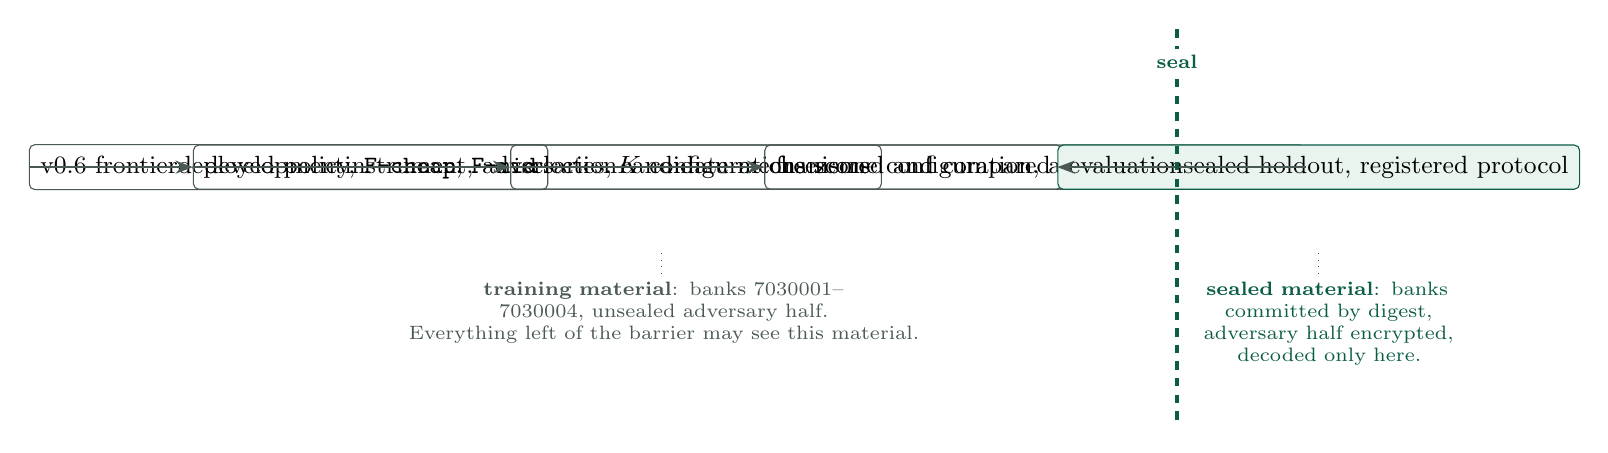
\begin{tikzpicture}[
  font=\small,
  st/.style={draw=fishgray,rounded corners=2pt,inner sep=4pt},
  seal/.style={st,fill=fishlight,draw=fishgreen},
  note/.style={inner sep=0pt,font=\scriptsize,align=center},
  arr/.style={-{Stealth[length=2.2mm]},fishgray,thick}]
% The gap before evaluation is wider than the other three, because the seal
% barrier passes between freeze and evaluation and must touch neither box, and
% the sealed-material note has to begin clear of it.  The whole picture is
% 461pt wide against a 468pt text block.
\node[st]   (base) at (0,0)      {\stage{v0.6 frontier}{deployed policy,\\[-1pt] \texttt{F-cheap}, \texttt{F-mid}}};
\node[st]   (dev)  at (3.161,0)  {\stage{development}{instrument, adversaries,\\[-1pt] candidate mechanisms}};
\node[st]   (sel)  at (6.322,0)  {\stage{selection}{$K$ configurations\\[-1pt] scored and compared}};
\node[st]   (frz)  at (9.483,0)  {\stage{freeze}{one configuration,\\[-1pt] artifact round-tripped}};
\node[seal] (ev)   at (13.084,0) {\stage{evaluation}{sealed holdout,\\[-1pt] registered protocol}};
\draw[arr] (base) -- (dev); \draw[arr] (dev) -- (sel); \draw[arr] (sel) -- (frz); \draw[arr] (frz) -- (ev);
% The barrier, midway between freeze and evaluation.  Its label is set above
% the row on a white ground, so the dashes stop at the word rather than
% running through it: nothing in this figure is drawn on top of anything else.
\draw[fishgreen,very thick,dashed] (11.2835,1.75) -- (11.2835,-3.25);
\node[fishgreen,font=\scriptsize\bfseries,fill=white,inner sep=2pt] at (11.2835,1.34) {seal};
% Both notes hang from the same depth, so their first lines align.  The sealed
% note begins to the right of the barrier and never crosses it.
\node[note,fishgray,text width=68mm,anchor=north] (train) at (4.7415,-1.45)
  {\textbf{training material}: banks 7030001--7030004, unsealed adversary half.\\
   Everything left of the barrier may see this material.};
\node[note,fishgreen,text width=33mm,anchor=north west] (hold) at (11.5335,-1.45)
  {\textbf{sealed material}: banks committed by digest, adversary half encrypted, decoded only here.};
\draw[fishgray,dotted]  (4.7415,-1.09) -- (4.7415,-1.41);
\draw[fishgreen,dotted] (13.084,-1.09) -- (13.084,-1.41);
\end{tikzpicture}
\caption{The development and evaluation protocol. Configurations were generated, scored and selected
using training material only. Exactly one configuration was then frozen, and evaluated against
material whose digests had been committed before any candidate existed, under a protocol registered in
advance (\S\ref{sec:evaluation-seal}). The seal is enforced by the engine rather than by convention:
a run naming a sealed seed fails unless an explicit variable is set, which was set once and recorded.}
\label{fig:protocol}
\end{figure}

\subsection{Material, and the checks performed before any measurement}
\label{sec:design-material}

All \vsevenBanks{} bank digests reproduce, at \vsevenBankDeals{} deals each (Table~\ref{tab:banks}). The sealed adversary half
decodes to \vsevenSealedRows{} configurations whose plaintext SHA-256 matches the commitment recorded
at sealing. The frozen configuration's artifact verifies, its specification rebuilding character for
character from its own ordered option map, and its round trip with search enabled is identical over
\vsevenRtwoaGames{} games. The engine's soundness audit reports \vsevenVerifyViolations{} violations
in \vsevenVerifyChecks{} checks and its self-test passes on \vsevenSelftestChecks{} checks.

\begin{table}[!ht]\centering
\caption{The deal banks. Each digest was recomputed before any cell was played, by folding the six
dealt hands and the dealer of every deal into a rolling hash without constructing a policy or playing
a game. The committed digests had been computed by a different build of the engine at sealing time,
so agreement is between two binaries as well as two dates.}
\label{tab:banks}
{\tabfont\begin{tabular}{lrlc}
\toprule
Bank & Deals & Digest reproduced & Matches commitment \\
\midrule
7090001 & 24,000 & \texttt{896dbc89be124d85} & \checkmark \\
7090002 & 24,000 & \texttt{0b6e40d834ac0ca1} & \checkmark \\
7090003 & 24,000 & \texttt{863bea69baf6e73c} & \checkmark \\
7090004 & 24,000 & \texttt{54f257c3f8ae9fab} & \checkmark \\
7090005 & 24,000 & \texttt{268a1dae71a31713} & \checkmark \\
7091001 & 24,000 & \texttt{958ada042cc26900} & \checkmark \\
7091002 & 24,000 & \texttt{5c39af3b5e0bd9a0} & \checkmark \\
\bottomrule
\end{tabular}}
\end{table}

\begin{table}[!ht]\centering
\caption{Calibration of the side-channel controls on holdout material. \emph{Must fail} is the set
the protocol names for each planted violation in advance. It is not one test each: the seed cheat is
visible to two of them. A control failing a test outside its set, or missing one inside it, would
mean the gate does not discriminate.}
\label{tab:sidechannel}
{\tabfont\begin{tabular}{lccccl c}
\toprule
Planted channel & S3 & S4 & S5 & S6 & Must fail & As required \\
\midrule
\texttt{v07x:cheat=seed} & PASS & FAIL & FAIL & PASS & S4, S5 & \checkmark \\
\texttt{v07x:cheat=shared} & PASS & PASS & PASS & FAIL & S6 & \checkmark \\
\texttt{v07x:cheat=conv} & FAIL & PASS & PASS & PASS & S3 & \checkmark \\
\bottomrule
\end{tabular}}
\end{table}

The homogeneity controls of \S\ref{sec:evaluation-side} calibrate as specified: each planted violation
fails exactly the tests named for it and no others, identically on both banks, over
\vsevenSideCells{} cells (Table~\ref{tab:sidechannel}).

\subsection{The soundness gate}
\label{sec:design-gate}

\sestina{} passes all \vsevenGateRulesWord{} rules of Table~\ref{tab:gate}: \vsevenGateDeadAsks\% provably dead asks against a
0.10\% bar, longest dead run \vsevenGateLongestDead{}, mirror tail maximum \vsevenGateTailMax{} with
99th percentile \vsevenGateTailPnn{}, and \vsevenGateSsix{} seat-isolation mismatches over
\vsevenGateSsixNodes{} audited decisions. Reported but not gated: \vsevenGateEvents{} events per game,
\vsevenGateAskHit\% ask hit rate and \vsevenGateMisdecl\% misdeclaration. The negative control fails
\vsevenNegFailCount{} rules, namely \vsevenNegFails{}, which are exactly the rules the protocol names
for it in advance.

\begin{table}[!ht]\centering
\caption{The soundness gate, \vsevenGateRulesWord{} rules, run on training material by design. The negative control is
a configuration constructed to be rejected.}
\label{tab:gate}
{\tabfont\begin{tabular}{lcccc}
\toprule
Rule & SESTINA v1.0 & v0.6 & \texttt{F-cheap} & Negative control \\
\midrule
provably-dead asks $\le 0.10\%$ & ok & ok & ok & \textbf{fail} \\
longest dead run $\le 5$ & ok & ok & ok & \textbf{fail} \\
games with a run $\ge 6$ = 0 & ok & ok & ok & \textbf{fail} \\
action-limit games = 0 & ok & ok & ok & \textbf{fail} \\
mirror tail max $< 220$, p99 $\le 150$ & ok & ok & ok & \textbf{fail} \\
declarations at/after event 220 = 0 & ok & ok & ok & ok \\
S3/S4/S5 certified, zero tolerance & ok & ok & ok & ok \\
S6 = 0 at \texttt{-{}-threads=1 -{}-freshagents} & ok & ok & ok & ok \\
\midrule
\textbf{verdict} & \textbf{PASS} & \textbf{PASS} & \textbf{PASS} & \textbf{FAIL} \\
\bottomrule
\end{tabular}}
\end{table}

\subsection{The registered protocol}
\label{sec:design-protocol}

The protocol fixed, before any holdout deal was played: the primary comparison target (\fcheap{},
for the reason in \S\ref{sec:development-frontier}); the primary decision rule; seven secondary
claims each with its own threshold; and seven conditions that would constitute non-confirmation.
Appendix~\ref{app:thresholds} reproduces them.

The primary decision rule is worth stating in the body, because the paper avoids the word
\emph{certified} in favour of naming what was actually satisfied. The registered rule was that the
comparison against \fcheap{} would be regarded as a confirmed advance if the pooled edge had a lower
bound above \vsevenPrimaryFloor{}~pp, \emph{and} the sign replicated on both banks, \emph{and} the
configuration passed the soundness gate. A pooled edge positive with a lower bound below
\vsevenPrimaryFloor{} but above zero, with the sign replicating, would be recorded as a measured but
unconfirmed advance; an interval containing zero, a sign that did not replicate, or a gate failure
would be recorded as no advance.

The protocol also fixed in advance the sentence to be used if the partner-regime comparison retained
a particular ordering, so that its direction could not be chosen after the fact, and recorded that on
training material that comparison ran \emph{against} \sestina{}. \S\ref{sec:results-partners}
reports the outcome and uses the registered wording.

\subsection{The battery}
\label{sec:design-battery}

\vsevenScoredCells{} scored cells over \vsevenScoredGames{} games (Table~\ref{tab:battery}). No registered cell was dropped;
\vsevenCellsAdded{} were added, and Appendix~\ref{app:deviations} records why.

\begin{table}[!ht]\centering
\caption{Every registered battery against what was measured. \emph{Registered} is the count the
protocol names, not the count that ran: two deviations add a reference cell and sixteen control cells,
because without them three of the protocol's own questions are not computable from the cells it
lists.}
\label{tab:battery}
{\tabfont\begin{tabularx}{\linewidth}{@{}l L r r r l@{}}
\toprule
Battery & What it measures & Registered & Added & Measured & Status \\
\midrule
B2 & headline strength against the frontier & 10 & 0 & 10 & complete \\
B3 & the shared 31-member panel & 248 & 0 & 248 & complete \\
B4 & a fresh adversary search & 16 & 0 & 16 & complete \\
B5 & the attribution lattice & 22 & 2 & 24 & complete (D1) \\
B6 & the partner-regime table & 64 & 0 & 64 & complete \\
B7 & cross-play between independent runs & 24 & 0 & 24 & complete \\
B8 & the rule-dialect table & 16 & 0 & 16 & complete \\
B9 & the negative controls & 10 & 16 & 26 & complete (D2) \\
B10 & the S6 residual & 16 & 0 & 16 & complete \\
\bottomrule
\end{tabularx}}
\end{table}

Scored cells carry no soundness-audit evidence, and this paper does not imply otherwise. The match
harness does not run the audit, so the audit check count is \vsevenAuditChecks{} in all
\vsevenScoredCells{} of them, and a report of zero violations over a scored cell would be zero out of
zero. The engine-wide audit figure quoted in \S\ref{sec:inference-verify} and
\S\ref{sec:design-material} comes from the dedicated verification run and is not restated as a
property of the battery.
%% --- end sections_v07/10-design ---
%% --- begin sections_v07/11-results ---
\section{Results}
\label{sec:results}

Every holdout measurement in this section is produced from the artifacts by the generator
described in Appendix~\ref{app:repro} and emitted into this document mechanically. The figures those
measurements are read against are not measurements of this holdout: registered expectations,
earlier cycles' results, and structural counts. Appendix~\ref{app:repro} records where each comes
from. The section answers RQ1 in
\S\ref{sec:results-primary}, RQ3 in \S\ref{sec:results-attribution}, and RQ2 in
\S\ref{sec:results-partners} through \S\ref{sec:results-adversarial}, before reporting the validity
controls and the computational cost.

\subsection{RQ1: strength against the v0.6 frontier}
\label{sec:results-primary}

Against \fcheap{}, the registered primary target, \sestina{} gains
\textbf{\vsevenBtwoFcheapMag{}~pp} of win-rate edge $[\vsevenBtwoFcheapLo, \vsevenBtwoFcheapHi]$ over
\vsevenBtwoFcheapN{} games, with the sign replicating on both banks
(\vsevenBtwoFcheapBankOne{} and \vsevenBtwoFcheapBankTwo{}) and the lower bound above the registered
\vsevenPrimaryFloor{}~pp threshold. The configuration passed the soundness gate
(\S\ref{sec:design-gate}). All three conditions of the registered primary decision rule are therefore
satisfied, and the comparison \vsevenPrimaryVerdict{}. Figure~\ref{fig:forest} places that
comparison and the others on one axis, and Table~\ref{tab:frontier} gives the cells behind it.

\begin{figure}[!ht]\centering
{\tabfont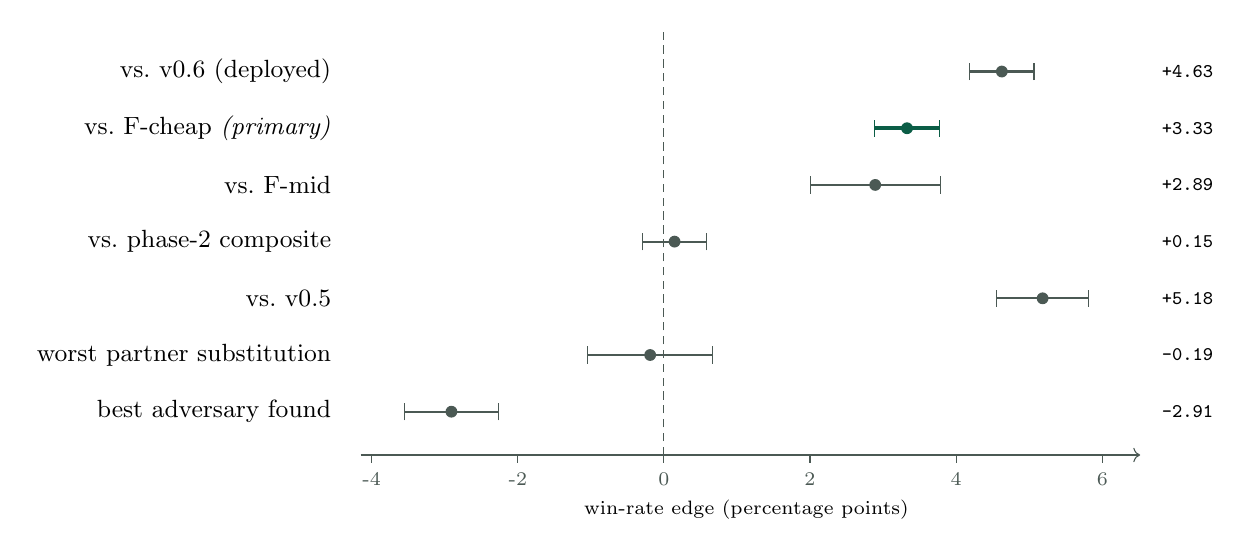
\begin{tikzpicture}[x=1cm,y=1cm]
  \node[anchor=east,font=\small] at (-0.25,-0.000) {vs.\ v0.6 (deployed)};
  \draw[fishgray,thick] (7.735,-0.000) -- (8.551,-0.000);
  \draw[fishgray] (7.735,-0.110) -- (7.735,0.110);
  \draw[fishgray] (8.551,-0.110) -- (8.551,0.110);
  \fill[fishgray] (8.143,-0.000) circle (0.075);
  \node[anchor=west,font=\scriptsize\ttfamily] at (10.050,-0.000) {+4.63};
  \node[anchor=east,font=\small] at (-0.25,-0.720) {vs.\ F-cheap \textit{(primary)}};
  \draw[fishgreen,ultra thick] (6.522,-0.720) -- (7.355,-0.720);
  \draw[fishgreen] (6.522,-0.830) -- (6.522,-0.610);
  \draw[fishgreen] (7.355,-0.830) -- (7.355,-0.610);
  \fill[fishgreen] (6.939,-0.720) circle (0.075);
  \node[anchor=west,font=\scriptsize\ttfamily] at (10.050,-0.720) {+3.33};
  \node[anchor=east,font=\small] at (-0.25,-1.440) {vs.\ F-mid};
  \draw[fishgray,thick] (5.709,-1.440) -- (7.360,-1.440);
  \draw[fishgray] (5.709,-1.550) -- (5.709,-1.330);
  \draw[fishgray] (7.360,-1.550) -- (7.360,-1.330);
  \fill[fishgray] (6.535,-1.440) circle (0.075);
  \node[anchor=west,font=\scriptsize\ttfamily] at (10.050,-1.440) {+2.89};
  \node[anchor=east,font=\small] at (-0.25,-2.160) {vs.\ phase-2 composite};
  \draw[fishgray,thick] (3.578,-2.160) -- (4.395,-2.160);
  \draw[fishgray] (3.578,-2.270) -- (3.578,-2.050);
  \draw[fishgray] (4.395,-2.270) -- (4.395,-2.050);
  \fill[fishgray] (3.987,-2.160) circle (0.075);
  \node[anchor=west,font=\scriptsize\ttfamily] at (10.050,-2.160) {+0.15};
  \node[anchor=east,font=\small] at (-0.25,-2.880) {vs.\ v0.5};
  \draw[fishgray,thick] (8.079,-2.880) -- (9.243,-2.880);
  \draw[fishgray] (8.079,-2.990) -- (8.079,-2.770);
  \draw[fishgray] (9.243,-2.990) -- (9.243,-2.770);
  \fill[fishgray] (8.661,-2.880) circle (0.075);
  \node[anchor=west,font=\scriptsize\ttfamily] at (10.050,-2.880) {+5.18};
  \node[anchor=east,font=\small] at (-0.25,-3.600) {worst partner substitution};
  \draw[fishgray,thick] (2.883,-3.600) -- (4.472,-3.600);
  \draw[fishgray] (2.883,-3.710) -- (2.883,-3.490);
  \draw[fishgray] (4.472,-3.710) -- (4.472,-3.490);
  \fill[fishgray] (3.677,-3.600) circle (0.075);
  \node[anchor=west,font=\scriptsize\ttfamily] at (10.050,-3.600) {-0.19};
  \node[anchor=east,font=\small] at (-0.25,-4.320) {best adversary found};
  \draw[fishgray,thick] (0.557,-4.320) -- (1.749,-4.320);
  \draw[fishgray] (0.557,-4.430) -- (0.557,-4.210);
  \draw[fishgray] (1.749,-4.430) -- (1.749,-4.210);
  \fill[fishgray] (1.153,-4.320) circle (0.075);
  \node[anchor=west,font=\scriptsize\ttfamily] at (10.050,-4.320) {-2.91};
  \draw[densely dashed,fishgray] (3.851,-4.870) -- (3.851,0.550);
  \draw[->,fishgray] (0,-4.870) -- (9.900,-4.870);
  \draw[fishgray] (0.140,-4.870) -- (0.140,-4.970) node[below,font=\scriptsize] {-4};
  \draw[fishgray] (1.996,-4.870) -- (1.996,-4.970) node[below,font=\scriptsize] {-2};
  \draw[fishgray] (3.851,-4.870) -- (3.851,-4.970) node[below,font=\scriptsize] {0};
  \draw[fishgray] (5.707,-4.870) -- (5.707,-4.970) node[below,font=\scriptsize] {2};
  \draw[fishgray] (7.563,-4.870) -- (7.563,-4.970) node[below,font=\scriptsize] {4};
  \draw[fishgray] (9.419,-4.870) -- (9.419,-4.970) node[below,font=\scriptsize] {6};
  \node[font=\scriptsize,anchor=north] at (4.900,-5.320) {win-rate edge (percentage points)};
\end{tikzpicture}}
\caption{Principal comparisons for \sestina{}, pooled over both holdout banks with 95\%
deal-clustered bootstrap confidence intervals. Positive values favour \sestina{}. The registered
primary comparison is highlighted. The bottom two rows place two robustness results on the same
axis: the worst partner substitution of \S\ref{sec:results-partners}, and the most successful of the
\vsevenBfourArms{} adversarial searches of \S\ref{sec:results-adversarial}.}
\label{fig:forest}
\end{figure}

\begin{table}[!ht]\centering
\caption{Strength against the \vsix{} frontier and lineage baselines, paired duplicate blocks, both
holdout banks.}
\label{tab:frontier}
{\tabfont\begin{tabular}{llrrrr}
\toprule
Cell & Opponent & Edge (pp) & 95\% CI & Games & Sign replicates \\
\midrule
B2.1 & v0.6 & $+4.63$ & $[+4.19, +5.06]$ & 48,000 & yes \\
B2.2 & \texttt{F-cheap} & $+3.33$ & $[+2.88, +3.78]$ & 48,000 & yes \\
B2.3 & \texttt{F-mid} & $+2.89$ & $[+2.00, +3.78]$ & 12,000 & yes \\
B2.4 & the phase-2 composite & $+0.15$ & $[-0.29, +0.59]$ & 48,000 & yes \\
B2.5 & v0.5 & $+5.18$ & $[+4.56, +5.81]$ & 24,000 & yes \\
\bottomrule
\end{tabular}}
\end{table}

Against the lineage baselines, \sestina{} gains \vsevenBtwoIncumbent{}~pp over the deployed
\vsix{} policy $[\vsevenBtwoIncumbentLo, \vsevenBtwoIncumbentHi]$, \vsevenBtwoFmid{}~pp over \fmid{}
$[\vsevenBtwoFmidLo, \vsevenBtwoFmidHi]$, and \vsevenBtwoVfive{}~pp over v0.5.

\textbf{Against \composite{} it gains \vsevenBtwoComposite{}~pp
$[\vsevenBtwoCompositeLo, \vsevenBtwoCompositeHi]$, an interval containing zero.}
\S\ref{sec:results-composite} treats that result, which the protocol had named in advance as a
condition of non-confirmation.

\paragraph{Declaration accuracy is reported without a claim.} The declaration-family floor applies to
the declaration-accuracy column. The harness emits declaration accuracy as a bare rate with no
interval of any kind, so no interval can be quoted and no claim about the declaration channel is
made. \sestina{} runs \vsevenDeclFrozenLo{} to \vsevenDeclFrozenHi{} across the five cells against
opponents' \vsevenDeclOppLo{} to \vsevenDeclOppHi{}. That is a diagnostic.

\subsection{Non-confirmatory results}
\label{sec:results-nonconfirm}

The protocol named seven conditions in advance that would constitute non-confirmation, because after
the data are in every one of them admits a reading that makes it sound like something else. Two arose,
and they are reported here rather than in a discussion of caveats.

\subsubsection{\sestina{} does not measurably outperform the phase-2 composite}
\label{sec:results-composite}

\sestina{} against \composite{} is \vsevenBtwoComposite{}~pp
$[\vsevenBtwoCompositeLo, \vsevenBtwoCompositeHi]$ over \vsevenBtwoCompositeN{} games. Both banks are
positive, so the sign replicates, but the interval contains zero.

The registered interpretation is explicit, and this paper adopts it. The increment that an earlier
phase had reported over the composite, \vsevenKthreeOverComposite{}
$[\vsevenKthreeOverCompositeLo, \vsevenKthreeOverCompositeHi]$ on a single bank, did not replicate;
on this comparison \sestina{} reduces to a configuration that development phase 2 had already
assembled.

The arithmetic makes the cell interpretable rather than merely disappointing. \sestina{} minus
\composite{} is exactly the tie-break repair, the urgency removal and the stall detector added, with
one further switch removed. \S\ref{sec:results-attribution} measures the stall detector's
contribution as identically zero, and the removed switch's leave-one-out drop was zero on training
material. The protocol states that group's training value in advance as \vsevenTrainGroup{}
$[\vsevenTrainGroupLo, \vsevenTrainGroupHi]$; on holdout it is \vsevenBtwoComposite{}
$[\vsevenBtwoCompositeLo, \vsevenBtwoCompositeHi]$.

What this does and does not license is worth stating precisely, because \fcheap{} and \composite{}
are different objects (Table~\ref{tab:configs}). It does not retract
\S\ref{sec:results-primary}: \fcheap{} is a configuration of the \vsix{} frontier that existed before
this cycle, and \sestina{} improves on it by a replicated margin. What it licenses is the narrower
statement that \textbf{the strength gain in this cycle is real and was produced in development phase
2, and the architecture work that followed added no measurable strength on top of it}.

\subsubsection{The attribution location test does not replicate}
\label{sec:results-location}

The protocol's third non-confirmation condition is that the lattice cannot locate the gain: if
removing every single component in turn costs less than a third of the whole, the configuration has a
gain it cannot explain. Read per bank, as \S\ref{sec:evaluation-replication} requires, the two banks
disagree (Table~\ref{tab:location}).

\begin{table}[!ht]\centering
\caption{The attribution location test, read per bank. \emph{Whole} is the measured whole,
\emph{one third} the protocol's threshold, and \emph{largest single drop} the biggest
leave-one-out drop the lattice contains.}
\label{tab:location}
{\tabfont
\begin{tabular}{lrrlc}
\toprule
Bank & Whole & One third & Largest single drop & Verdict \\
\midrule
7090001 & \vsevenLocWholeOne{} & \vsevenLocThirdOne{} & \texttt{\vsevenLocAtOne{}} \vsevenLocBiggestOne{} & \vsevenLocVerdictOne{} \\
7090003 & \vsevenLocWholeThree{} & \vsevenLocThirdThree{} & \texttt{\vsevenLocAtThree{}} \vsevenLocBiggestThree{} & \vsevenLocVerdictThree{} \\
\bottomrule
\end{tabular}}
\end{table}

The two banks' largest drops differ by \vsevenLocSplit{}~pp against a half-width on that difference of
comparable size, so the split is real on the point estimates and is not itself statistically resolved.
Under the replication criterion the pooled verdict is not replicated
(\vsevenLocReplicates{}), and the honest reading is that this battery does not settle whether the gain
is located by the protocol's one-third rule. Note that the disagreement is between verdict labels
rather than between signs, which is itself a recorded extension of the criterion. The sub-additivity
claim of \S\ref{sec:results-attribution} passes on both banks; it is the location test specifically
that splits.

\subsubsection{The selection check}
\label{sec:results-selection}

\vsevenSelK{} configurations were scored against the deployed policy during development. At the
lattice cell size the per-cell standard deviation is \vsevenSelSigma{}~pp, so the quantity the protocol registers as the expected maximum of
\vsevenSelK{} draws under the null that none differs from the reference is
$\sigma\sqrt{2\ln K} = \vsevenSelExpectedMax{}$~pp, which is an upper bound on that
expectation rather than the expectation itself.

The selection term on holdout material is \vsevenSelOnHoldout{}~pp \emph{by construction}: the holdout
banks were never available for selection, so not one of the \vsevenSelK{} choices could have used any
deal of them. That is a structural guarantee rather than a measurement.
Table~\ref{tab:selection} sets the four registered quantities against their holdout measurements.

\begin{table}[!ht]\centering
\caption{The four quantities the registered selection check tabulates, against their holdout
measurements. Three reproduce or exceed; one falls short. These are not every figure the protocol
states in advance, and two of the partner-regime predictions in \S\ref{sec:results-partners} also
come in low.}
\label{tab:selection}
{\tabfont\begin{tabular}{lrrr}
\toprule
Quantity & Training & Holdout & Shortfall \\
\midrule
B2.4 --- \texttt{rtie} + urgency-off + \texttt{stall}, as a group & $+0.78$ & $+0.15$ & $-0.63$ \\
B6 self-play row, opponent \texttt{v05} & $+2.94$ & $+4.49$ & $+1.55$ \\
B7 diagonal (self-play) & $+4.51$ & $+4.55$ & $+0.04$ \\
B7 off-diagonal (cross-play) & $+4.48$ & $+4.55$ & $+0.07$ \\
\bottomrule
\end{tabular}}
\end{table}

\vsevenSelReproduce{} of the four reproduce or exceed their training values. The largest shortfall,
\vsevenSelWorstShortfall{}~pp against the registered \vsevenSelExpectedMax{},
falls on the composite cell, which is precisely the quantity measuring the group of components the
configuration was selected over. That is the pattern the check was written to look for and it appears
where selection occurred. One quantity cannot establish that the group's training value was entirely
selection effect, and the check is not a formal correction
(\S\ref{sec:evaluation-multiplicity}); what it provides is a consistency test that the data pass in
the direction \S\ref{sec:results-composite} indicates.

\subsubsection{The seven conditions, answered}
\label{sec:results-seven}

Table~\ref{tab:seven} answers each of the seven in the protocol's own order.

\begin{table}[!ht]\centering
\caption{The seven registered non-confirmation conditions against what the holdout returned.
Appendix~\ref{app:thresholds} reproduces the conditions verbatim.}
\label{tab:seven}
{\tabfont
\begin{tabularx}{\linewidth}{@{}c L L@{}}
\toprule
\# & Condition & Result \\
\midrule
1 & the frontier comparison & not met. \vsevenBtwoFcheap{} $[\vsevenBtwoFcheapLo, \vsevenBtwoFcheapHi]$, sign replicates \\
2 & the composite comparison & \textbf{met.} \vsevenBtwoComposite{} $[\vsevenBtwoCompositeLo, \vsevenBtwoCompositeHi]$ \\
3 & attribution: the location test & \textbf{does not replicate.} \vsevenLocVerdictOne{} on one bank, \vsevenLocVerdictThree{} on the other \\
4 & brittleness under partner change or cross-play & not met. Minimum \vsevenSoneMin{}; cross-play off-diagonal minus diagonal \vsevenXpGap{} \\
5 & a successful adversary & not met. No search found a positive edge; largest upper bound \vsevenBfourWorstUpper{} \\
6 & the soundness gate & not met. All \vsevenGateRules{} rules pass \\
7 & the validity controls & not met. Every control behaves as specified \\
\bottomrule
\end{tabularx}}
\end{table}

Two of the seven are met or unresolved, being condition 2 outright and condition 3 by
non-replication. The other five are not met.

\subsection{Worst case and minimax regret over a shared panel}
\label{sec:results-panel}

\vsevenPanelCells{} cells. Four configurations were scored against the same
\vsevenPanelMembers{}-member panel on the same two banks: \vsevenPanelNear{} near-class members at
\vsevenDealsNear{} deals per bank, \vsevenPanelFar{} far-class archetypes at \vsevenDealsFar{}, and
\vsevenPanelExpensive{} expensive members at \vsevenDealsExpensive{}. All four carry a cell for every
member, which is what makes minimax regret defined. Table~\ref{tab:worstcase} gives each
configuration's worst cell.

\begin{table}[!ht]\centering
\caption{Worst panel cell per configuration. Per-bank values are given in bank order,
7090001 then 7090002.}
\label{tab:worstcase}
{\tabfont\begin{tabular}{llrcr}
\toprule
Configuration & Worst cell & Edge (pp) & 95\% CI & Per bank \\
\midrule
SESTINA v1.0 & phase-2 composite & $-0.04$ & $[-1.41, +1.33]$ & $+1.67$ / $-1.75$ \\
v0.6 deployed & \texttt{SEALED:X01xC3f} & $-4.24$ & $[-4.86, -3.62]$ & $-3.86$ / $-4.63$ \\
\texttt{F-cheap} & phase-2 composite & $-2.08$ & $[-3.48, -0.69]$ & $-2.21$ / $-1.96$ \\
phase-2 composite & phase-2 composite & $+0.00$ & $[+0.00, +0.00]$ & $+0.00$ / $+0.00$ \\
\bottomrule
\end{tabular}}
\end{table}

\sestina{}'s worst cell is \vsevenWorstFrozen{}~pp
$[\vsevenWorstFrozenLo, \vsevenWorstFrozenHi]$ against the deployed policy's \vsevenWorstIncumbent{}
$[\vsevenWorstIncumbentLo, \vsevenWorstIncumbentHi]$, satisfying the registered secondary claim that
the worst case not be catastrophic.

Two qualifications belong with that number, and both go against \sestina{}.

First, \textbf{it does not replicate in sign}. \sestina{}'s worst cell is
\vsevenWorstFrozenBankOne{} on the first bank and \vsevenWorstFrozenBankTwo{} on the second, attained
at a different panel member on each (\texttt{\vsevenWorstFrozenBankOneOpp{}} and
\texttt{\vsevenWorstFrozenBankTwoOpp{}}); on one bank \sestina{} has no negative cell anywhere on
the panel. Under the criterion of \S\ref{sec:evaluation-replication} the pooled value is not
replicated. What survives replication is the comparison the protocol actually gated on, since
\sestina{}'s worst cell is far above the deployed policy's on both banks, rather than the pooled
value itself.

Second, \textbf{it is not the best worst case of the four}. Configurations that are themselves panel
members carry a free zero cell against themselves, so the worst case is printed both ways;
\composite{} is ahead of \sestina{} on both readings, at \vsevenWorstComposite{} with its self-cell
and \vsevenWorstCompositeExSelf{} without.

\begin{table}[!ht]\centering
\caption{Minimax regret over the shared panel, best first. The protocol sets no threshold on this
quantity and requires only that it be reported.}
\label{tab:regret}
{\tabfont\begin{tabular}{lrr}
\toprule
Configuration & Minimax regret (pp) & Attained against \\
\midrule
\texttt{F-cheap} & 4.00 & v0.3 \\
phase-2 composite & 4.08 & \texttt{withholder} \\
SESTINA v1.0 & 4.53 & \texttt{withholder} \\
v0.6 deployed & 5.67 & \texttt{SEALED:X01xC3f} \\
\bottomrule
\end{tabular}}
\end{table}

\sestina{} is \textbf{\vsevenRegretFrozenRank{}rd of four} on minimax regret (Table~\ref{tab:regret}), at
\vsevenRegretFrozen{} against \vsevenRegretBest{}'s \vsevenRegretFcheap{} and \composite{}'s
\vsevenRegretComposite{}. The configuration with the best worst case is not the configuration with the
best regret, and this paper does not resolve the tension by selecting whichever statistic favours the
subject. The regret difference is concentrated in the far archetypes (Table~\ref{tab:farpanel}),
opponents every configuration already beats by between \vsevenFarSpanLo{} and \vsevenFarSpanHi{}~pp,
which is a reason to weight it less but not a reason to discount it.

\begin{table}[!ht]\centering
\caption{The far archetypes, where the minimax-regret differences are concentrated.}
\label{tab:farpanel}
{\tabfont\begin{tabular}{lrrrr}
\toprule
Far archetype & SESTINA v1.0 & v0.6 & \texttt{F-cheap} & Composite \\
\midrule
v0.3 & +28.72 & +25.47 & +24.72 & +28.40 \\
v0.2 & +34.32 & +31.68 & +32.67 & +33.17 \\
\texttt{lockout} & +30.78 & +28.65 & +28.97 & +29.07 \\
\texttt{detective} & +29.65 & +28.08 & +27.98 & +28.32 \\
\texttt{hunter} & +46.93 & +48.58 & +48.65 & +47.10 \\
\texttt{diversifier} & +43.40 & +44.90 & +45.18 & +43.32 \\
\texttt{bluffer} & +49.87 & +49.98 & +49.95 & +49.88 \\
\texttt{silent} & +32.75 & +34.23 & +34.05 & +30.92 \\
\texttt{withholder} & +25.35 & +29.88 & +29.55 & +25.80 \\
\texttt{random} & +50.00 & +50.00 & +50.00 & +50.00 \\
\bottomrule
\end{tabular}}
\end{table}

Against the hardest sealed adversary the ordering reverses: on
\texttt{\vsevenHardSealed{}}, \sestina{} scores \vsevenHardFrozen{}
$[\vsevenHardFrozenLo, \vsevenHardFrozenHi]$ where the deployed policy scores
\vsevenHardIncumbent{} and \fcheap{} scores \vsevenHardFcheap{}. \vsevenHardBeaters{} of the four
configurations beat that member with a lower bound above zero, namely \vsevenHardBeaterNames{}.

\paragraph{The panel mean, reported last and as a diagnostic.} Over the \vsevenPanelMembers{} shared
cells, which comprise \vsevenPanelDistinct{} distinct policies since three are named twice and are
therefore double-counted by any mean, the figures are \sestina{} \vsevenPanelMeanFrozen{},
\composite{} \vsevenPanelMeanComposite{}, \fcheap{} \vsevenPanelMeanFcheap{} and the deployed policy
\vsevenPanelMeanIncumbent{}. The reporting rule of \S\ref{sec:evaluation-panel} forbids leading with
this, and it points the opposite way from minimax regret. Appendix~\ref{app:panel} gives every cell.

\subsection{RQ3: attribution of the gain}
\label{sec:results-attribution}

The registered prediction was that the contestation weight of \S\ref{sec:agent-contest} carries the
gain, checkable as a leave-one-out drop of roughly two percentage points. On that check it holds: the holdout
drop is \vsevenLooRtwelve{}~pp $[\vsevenLooRtwelveLo, \vsevenLooRtwelveHi]$, with the training figure
\vsevenTrainRtwelveLoo{} inside the interval, and an add-one-in of \vsevenAddInRtwelve{}. The stronger
statement, that this coordinate is where the gain lives, is not supported at this power: the drop's
lower bound is \vsevenLooRtwelveLo{}, and \S\ref{sec:results-location} reports the protocol's own
location test failing to replicate. Table~\ref{tab:attribution} is the lattice.

\begin{table}[!ht]\centering
\caption{The attribution lattice. Add-one-in is measured from the deployed \vsix{} policy;
leave-one-out is the drop from \sestina{}. Reference cell \sestina{} against the deployed policy
on the lattice banks: \vsevenBfiveWhole{} $[\vsevenBfiveWholeLo, \vsevenBfiveWholeHi]$.}
\label{tab:attribution}
{\tabfont\begin{tabular}{lrcrc}
\toprule
Component & Add-one-in & 95\% CI & Leave-one-out & 95\% CI \\
\midrule
\texttt{r12=25} & $+2.18$ & $[+1.55, +2.81]$ & $+1.69$ & $[+0.80, +2.57]$ \\
\texttt{the search} & $+1.91$ & $[+1.38, +2.44]$ & $+0.57$ & $[-0.33, +1.46]$ \\
\texttt{rtie=1} & $+0.71$ & $[+0.08, +1.34]$ & $+1.08$ & $[+0.20, +1.97]$ \\
\texttt{urgency-off} & $+1.37$ & $[+1.12, +1.63]$ & $+0.64$ & $[-0.25, +1.53]$ \\
\texttt{stall=12} & $+0.00$ & $[+0.00, +0.00]$ & $+0.00$ & $[-0.89, +0.89]$ \\
\texttt{m2=0} \textit{(not in the freeze)} & $+0.77$ & $[+0.66, +0.88]$ & --- & --- \\
\bottomrule
\end{tabular}}
\end{table}

The stall detector behaves exactly as predicted. It is worth \vsevenAddInStall{}
$[\vsevenAddInStallLo, \vsevenAddInStallHi]$ added and \vsevenLooStall{} removed, bit-identical on
holdout in win rate and in events per game alike: the rule does not fire.

The naive sum of the five components \sestina{} carries is \vsevenBfiveSum{}~pp against a measured
whole of \vsevenBfiveWhole{}~pp, a sub-additivity ratio of \vsevenSubAdditivity{}
$[\vsevenSubAdditivityLo, \vsevenSubAdditivityHi]$, which contains the phase-2 composition figure of
\vsevenSubAddPhaseTwo{}. Quoting the sum would overstate the configuration by
\vsevenSubAdditivityOverstate{}~pp. The registered attribution claim, that components are
sub-additive and no single leave-one-out drop exceeds the whole, is satisfied.

One component was measured but is not carried by \sestina{}. The \texttt{m2} switch is worth
\vsevenAddInMtwo{} $[\vsevenAddInMtwoLo, \vsevenAddInMtwoHi]$ added to the blueprint, an interval
excluding zero and larger than the tie-break's add-one-in. Its zero leave-one-out drop was measured
on training material and is not re-measured here, because \sestina{} does not carry the switch and
the protocol directs that it not be added back; there is no leave-one-out cell for it and there could
not be.

\subsection{RQ2: partner substitution and one-seat upgrades}
\label{sec:results-partners}

\vsevenSonePositive{} of \vsevenSoneRows{} changed-partner rows against a v0.5 opponent are positive
(Table~\ref{tab:partners}). The minimum is
\vsevenSoneMin{} $[\vsevenOppFiveWithholderLo, \vsevenOppFiveWithholderHi]$, which is above the
registered $\vsevenSoneThreshold{}$ collapse threshold on the point estimate but \emph{not resolved
against it}, since the interval's lower bound falls below the threshold. This battery does not
separate a pass from a failure on the row that decides the claim, and reading a threshold from a
point estimate is a move this paper declines elsewhere (\S\ref{sec:results-controls}) and declines
here.

\begin{table}[!ht]\centering
\caption{Partner-regime table against a v0.5 opponent. Team A is the evaluated configuration plus two
copies of the named partner; team B is three copies of the opponent. Per-bank values are given in
bank order, 7090001 then 7090002.}
\label{tab:partners}
{\tabfont\begin{tabular}{lrcrc}
\toprule
Partners & SESTINA $-$ v0.6 & 95\% CI & Per bank & Repl. \\
\midrule
itself & $+4.49$ & $[+3.61, +5.38]$ & $+4.18$ / $+4.81$ & yes \\
v0.6 & $+1.93$ & $[+1.04, +2.82]$ & $+2.07$ / $+1.79$ & yes \\
v0.5 & $+0.78$ & $[-0.09, +1.66]$ & $+0.95$ / $+0.62$ & yes \\
v0.4 & $+1.34$ & $[+0.46, +2.22]$ & $+1.30$ / $+1.38$ & yes \\
v0.3 & $+1.40$ & $[+0.56, +2.25]$ & $+1.08$ / $+1.72$ & yes \\
\texttt{detective} & $+1.83$ & $[+0.97, +2.68]$ & $+1.35$ / $+2.30$ & yes \\
\texttt{withholder} & $-0.19$ & $[-1.04, +0.67]$ & $+0.00$ / $-0.38$ & \textbf{no} \\
\texttt{lockout} & $+1.89$ & $[+1.04, +2.74]$ & $+1.39$ / $+2.39$ & yes \\
\bottomrule
\end{tabular}}
\end{table}

Against a \vsix{} opponent all four rows are positive and clear zero
(Table~\ref{tab:partnerssix}), and this is where the measurement disagrees with the registered
expectation. The protocol states in advance \vsevenTrainOppSixSelf{} in self-play and
\vsevenTrainOppSixLo{} to \vsevenTrainOppSixHi{} under partner change. Measured:
\vsevenOppSixItself{} in self-play, and of the three changed rows two fall below the stated range,
namely \vsevenOppSixVthree{} against \texttt{v03}, more than a point below its floor, and
\vsevenOppSixDetective{} against \texttt{detective}.

\begin{table}[!ht]\centering
\caption{Partner-regime table against a \vsix{} opponent. Per-bank values are given in bank order,
7090001 then 7090002.}
\label{tab:partnerssix}
{\tabfont\begin{tabular}{lrcrc}
\toprule
Partners & SESTINA $-$ v0.6 & 95\% CI & Per bank & Repl. \\
\midrule
itself & $+4.55$ & $[+3.92, +5.18]$ & $+4.88$ / $+4.21$ & yes \\
v0.6 & $+2.75$ & $[+2.14, +3.37]$ & $+2.97$ / $+2.54$ & yes \\
v0.3 & $+1.46$ & $[+0.63, +2.29]$ & $+1.25$ / $+1.67$ & yes \\
\texttt{detective} & $+2.34$ & $[+1.49, +3.19]$ & $+2.42$ / $+2.26$ & yes \\
\bottomrule
\end{tabular}}
\end{table}

\begin{table}[!ht]\centering
\caption{Transfer across partners: \sestina{} over \vsix{} against \vsix{} over v0.5, on the same
eight settings and the same banks. The two training rows are quoted from the registered
protocol; the protocol records that its v0.6-over-v0.5
training row is computed on three of seven changed settings, so that row is not directly comparable
with the holdout row above it. Reported and not gated.}
\label{tab:regimes}
{\tabfont\begin{tabular}{lrrrr}
\toprule
Comparison & Min & Median & Self & Median/self \\
\midrule
SESTINA over v0.6 --- holdout & $-0.19$ & $+1.40$ & $+4.49$ & 0.313 \\
v0.6 over v0.5 --- holdout & $-0.40$ & $+0.26$ & $+0.69$ & 0.380 \\
SESTINA over v0.6 --- training, stated in advance & $-0.15$ & $+1.26$ & $+2.94$ & 0.428 \\
v0.6 over v0.5 --- training, stated in advance & $-0.61$ & $+0.64$ & $+1.35$ & 0.472 \\
\bottomrule
\end{tabular}}
\end{table}

The protocol stated in advance that if the ordering in Table~\ref{tab:regimes} survived, the
appropriate summary is that \sestina{}'s advantage transfers across partners about as well as
\vsix{}'s did and, on the median-to-self-play ratio, slightly less well. The ordering survived
(\vsevenSoneRatio{} against \vsevenBaseRatio{}), so that is the paper's summary. The fact it omits is
that \sestina{}'s absolute changed-partner median is \vsevenSoneMedian{} against \vsix{}'s
\vsevenBaseMedian{}, and the ratio is smaller mainly because the self-play row it divides by is more
than six times larger.

A one-seat upgrade is worth \vsevenOneSeatFive{}~pp against a v0.5 opponent (registered expectation
\vsevenTrainOneSeatFive{}) and \vsevenOneSeatSix{}~pp against a \vsix{} opponent (registered
\vsevenTrainOneSeatSix{}). That a single seat purchases a large fraction of the three-seat gain is
the strongest evidence in this paper that the advantage is individual rather than conventional.

\subsection{RQ2: cross-play between independently trained runs}
\label{sec:results-crossplay}

Diagonal mean \vsevenXpDiagonal{}, off-diagonal mean \vsevenXpOffDiagonal{}, off-diagonal minus
diagonal \vsevenXpGap{}~pp against a per-cell half-width of \vsevenXpHalfWidth{}. The worst off-diagonal cell
(\vsevenXpWorstOff{}) is \vsevenXpWorstOffShortfall{}~pp below the weakest diagonal cell
(\vsevenXpWeakestDiag{}), and the best off-diagonal (\vsevenXpBestOff{}) exceeds every diagonal cell.
The registered claim that the advantage is not a private convention between identical fits is
satisfied against a threshold of \vsevenStwoThreshold{}~pp. For scale, the coordination literature's
documented convention collapses run from self-play scores in the twenties to low single digits under
cross-play \cite{bard-hanabi,hu-otherplay}; nothing of that kind is present.
Table~\ref{tab:crossplay} is the cross-play matrix and Table~\ref{tab:crossh2h} the three pairs
head to head.

\begin{table}[!ht]\centering
\caption{Cross-play. Three runs of the same architecture, trained independently on disjoint fitting
banks with different search trajectories and, for one, a different starting basin; pairwise parameter
distance \vsevenXpDistanceLo{} to \vsevenXpDistanceHi{} over \vsevenCoordinates{} coordinates.}
\label{tab:crossplay}
{\tabfont\begin{tabular}{lccc}
\toprule
Run \textbackslash\ partners & xp1 & xp2 & xp3 \\
\midrule
xp1 & $+4.54$ $[+3.91, +5.17]$ & $+3.80$ $[+3.17, +4.42]$ & $+4.55$ $[+3.92, +5.19]$ \\
xp2 & $+4.93$ $[+4.29, +5.56]$ & $+4.91$ $[+4.29, +5.54]$ & $+4.83$ $[+4.20, +5.46]$ \\
xp3 & $+5.15$ $[+4.52, +5.78]$ & $+4.06$ $[+3.44, +4.69]$ & $+4.20$ $[+3.56, +4.83]$ \\
\bottomrule
\end{tabular}}
\end{table}

\begin{table}[!ht]\centering
\caption{The three independently trained runs head to head. \vsevenHtwohSeparated{} of the three
pairs separate from zero, which is what establishes that these are distinguishable policies rather
than one policy three times.}
\label{tab:crossh2h}
{\tabfont\begin{tabular}{lrr}
\toprule
Pair & Edge (pp) & 95\% CI \\
\midrule
xp1 vs xp2 & $+0.20$ & $[-0.43, +0.83]$ \\
xp1 vs xp3 & $+0.70$ & $[+0.08, +1.32]$ \\
xp2 vs xp3 & $+1.05$ & $[+0.43, +1.68]$ \\
\bottomrule
\end{tabular}}
\end{table}

\subsection{RQ2: robustness to rule dialects}
\label{sec:results-dialects}

Every row keeps its sign, every row replicates, and the largest excursion from the default row is
\vsevenDiaMaxExcursion{}~pp on \vsevenDiaMaxExcursionRow{}, inside the registered
\vsevenSfiveTolerance{}~pp tolerance. The advantage survives 48-card Literature, all three
arbitration orders, both declaration-permission changes and the full legacy dialect.
Table~\ref{tab:dialects} gives every row.

\begin{table}[!ht]\centering
\caption{The rule-dialect table. Both configurations play the same dialect in every row. Per-bank
values are given in bank order, 7090003 then 7090001. This is the first dialect sweep of its kind in
the corpus and has no training-bank counterpart.}
\label{tab:dialects}
{\tabfont\begin{tabular}{lrrrr}
\toprule
Dialect & Edge (pp) & 95\% CI & Per bank & vs default \\
\midrule
default & $+4.73$ & $[+4.10, +5.36]$ & $+4.57$ / $+4.88$ & $+0.00$ \\
no-out-of-turn & $+5.25$ & $[+4.63, +5.87]$ & $+4.72$ / $+5.78$ & $+0.52$ \\
no-cardless-declare & $+4.90$ & $[+4.27, +5.52]$ & $+4.71$ / $+5.08$ & $+0.17$ \\
maxasks=360 & $+4.73$ & $[+4.10, +5.36]$ & $+4.57$ / $+4.88$ & $+0.00$ \\
arb=high & $+4.85$ & $[+4.21, +5.49]$ & $+5.03$ / $+4.67$ & $+0.12$ \\
arb=turn & $+5.51$ & $[+4.88, +6.14]$ & $+5.26$ / $+5.77$ & $+0.78$ \\
sets=8 & $+4.13$ & $[+3.52, +4.73]$ & $+3.77$ / $+4.48$ & $-0.60$ \\
legacy & $+5.12$ & $[+4.50, +5.75]$ & $+4.62$ / $+5.63$ & $+0.40$ \\
\bottomrule
\end{tabular}}
\end{table}

Two readings belong with the table. The \texttt{maxasks} row is bit-identical to the default
(\vsevenMaxasksIdentical{}), because the 400-ask cap is never reached in this population, so it
measures nothing. Consequently the legacy residual, which the protocol assigns to the forced-endgame
willingness ladder for want of a flag of its own, is arithmetically legacy minus two effective
components rather than three; it is \vsevenLegacyResidual{}
$[\vsevenLegacyResidualLo, \vsevenLegacyResidualHi]$, an interval \vsevenLegacyResidualRatio{} times
the size of the residual, so the data are equally consistent with the ladder contributing nothing.

\subsection{RQ2: adversarial search against \sestina{}}
\label{sec:results-adversarial}

\vsevenBfourFits{} of \vsevenBfourArmsWord{} searches produced a weight vector and all
\vsevenBfourArmsWord{} were evaluated. \textbf{None of the \vsevenBfourArmsWord{} searches found a positive
edge against \sestina{} at the tested budgets.} Every one loses, by between
\vsevenBfourBestLoss{} and \vsevenBfourWorstLoss{}~pp; every sign replicates; and the largest upper
bound anywhere is \vsevenBfourWorstUpper{}, which is \vsevenBfourFloorGap{}~pp below the detection
floor. The registered claim is satisfied. Table~\ref{tab:adversaries} gives every search.

\begin{table}[!ht]\centering
\caption{\vsevenBfourArms{} independently constructed adversarial searches against \sestina{}. A
positive edge would mean the adversary beats the target. Each was fitted on a deal stream disjoint
from the banks it is evaluated on. Per-bank values are given in bank order, 7090001 then 7090002.}
\label{tab:adversaries}
{\tabfont\begin{tabularx}{\linewidth}{@{}l L l r c r c@{}}
\toprule
ID & Class & Objective & Edge (pp) & 95\% CI & Per bank & Repl. \\
\midrule
Z01 & C1 in-class & win & $-2.91$ & $[-3.55, -2.27]$ & $-2.76$ / $-3.06$ & yes \\
Z02 & C2 extended & win & $-3.90$ & $[-4.52, -3.28]$ & $-3.80$ / $-4.00$ & yes \\
Z03 & C1 & declerr & $-10.70$ & $[-11.32, -10.09]$ & $-10.65$ / $-10.76$ & yes \\
Z04 & C1 & events & $-9.64$ & $[-10.27, -9.01]$ & $-9.83$ / $-9.46$ & yes \\
Z05 & C1 & forced & $-7.14$ & $[-7.76, -6.52]$ & $-7.17$ / $-7.11$ & yes \\
Z06 & C2 wide sigma & win & $-5.25$ & $[-5.88, -4.62]$ & $-4.93$ / $-5.57$ & yes \\
Z07 & C1 v05 basin & win & $-5.21$ & $[-5.84, -4.58]$ & $-4.85$ / $-5.58$ & yes \\
Z08 & C5 white-box & win & $-3.56$ & $[-4.19, -2.92]$ & $-3.95$ / $-3.17$ & yes \\
\bottomrule
\end{tabularx}}
\end{table}

The searches control all three opposing seats, run in the synchronised correlation regime, and use a
budget of \vsevenBfourGens{} generations of a \vsevenBfourPop{}-member population at
\vsevenBfourDeals{} deals per candidate. They maximise four different objectives, being win rate,
declaration error, event count and forced-endgame incidence, and two of them depart deliberately from
the template, one using a wide search variance and one seeded in the v0.5 basin, so that the set is
not one search repeated. The declaration-objective arm is read against the declaration-family floor of
\vsevenDeclFloor{} rather than the general floor.

This is a lower bound on exploitability and not an upper bound. It is evidence about these searches
at these budgets in these classes, and \S\ref{sec:discussion-exploit} states what would be required
to convert it into a statement about \sestina{}.

\subsubsection{The white-box transcript-inversion adversary}
\label{sec:results-whitebox}

\texttt{Zeight} is the adversary class the threat model of \S\ref{sec:threat} was written for: an
opponent that reads the target's own deterministic policy and reconstructs the deal posterior from
the public transcript, testing directly whether common-knowledge coordination among identical
deterministic teammates exposes exploitable behavioural information. It reaches
\vsevenZeightEdge{}~pp $[\vsevenZeightLo, \vsevenZeightHi]$, a replicated loss.

Three limits belong with that cell, since it is the one a sceptical reader should weigh most
heavily. The inverter the base fixes queries a \vsix{} model of the target rather than the frozen
configuration itself, a setting carried forward from the phase whose target \emph{was} \vsix{}, so
the likelihood is computed against a policy that does not search, leaves the urgency escalation on,
and carries neither the tie-break nor the contestation coordinate; the corpus does not measure how
far that model's choice diverges from the frozen target's, so the size of the resulting degradation
is unquantified. \vsevenZeightInert{} of its fitted coordinates are inert, because the white-box base derives from the
\vsix{} agent and reads only that policy's \vsevenVsixCoords{} coordinates while the search extends
its vector to \vsevenCoordinates{}; the effective search is therefore over \vsevenZeightLive{} live
coordinates plus the inverter the base fixes. And the budget is small. The result is evidence that
this inverter, at this budget, does not exploit \sestina{}; it is not evidence that no white-box
attack can.

\paragraph{Fitting performance is not evaluation performance.} The in-class arm reaches
\vsevenZoneFitMargin{}~pp of paired margin in its final generation on its own fitting stream, and
\vsevenZoneFitPeak{}~pp at its best generation, before landing at \vsevenZoneEdge{}~pp on disjoint
banks. Most of that difference is not the change of bank: the same run re-scores its selected vector
on the fitting stream and already falls below parity there, because the generation figure is a
maximum over candidates at \vsevenBfourDeals{} deals each rather than a measurement of the vector
that was retained. Re-evaluation closes most of the gap and disjoint banks close the rest.

\subsection{Validity controls}
\label{sec:results-controls}

If these misbehave, nothing else in this section is interpretable. Table~\ref{tab:controls} is the
planted-edge recovery.

\begin{table}[!ht]\centering
\caption{Planted-edge recovery. The recovered excess is the responder's edge against the handicapped
target minus its edge against the unhandicapped one. The sub-floor rung must \emph{not} be recovered.}
\label{tab:controls}
{\tabfont\begin{tabularx}{\linewidth}{@{}l C C C C@{}}
\toprule
Planted handicap & Planted cost & vs.\ handicapped & vs.\ SESTINA & Recovered excess \\
\midrule
0.05 \textit{(sub-floor)} & \ci{$+0.78$}{+0.25, +1.32} & \ci{$-3.62$}{-4.26, -2.99} & \ci{$-4.32$}{-4.94, -3.69} & \ci{$\mathbf{+0.70}$}{-0.20, +1.59} \\\addlinespace[0.9ex]
0.08 & \ci{$+1.59$}{+1.05, +2.13} & \ci{$-2.29$}{-2.92, -1.67} & \ci{$-4.67$}{-5.30, -4.05} & \ci{$\mathbf{+2.38}$}{+1.50, +3.26} \\\addlinespace[0.9ex]
0.11 & \ci{$+8.52$}{+7.93, +9.12} & \ci{$+2.52$}{+1.89, +3.16} & \ci{$-6.90$}{-7.52, -6.28} & \ci{$\mathbf{+9.42}$}{+8.54, +10.31} \\\addlinespace[0.9ex]
0.15 & \ci{$+11.44$}{+10.85, +12.03} & \ci{$+7.30$}{+6.68, +7.93} & \ci{$-5.34$}{-5.97, -4.71} & \ci{$\mathbf{+12.64}$}{+11.75, +13.53} \\
\bottomrule
\end{tabularx}}
\end{table}

Two of the three supra-floor rungs are recovered with a lower bound above the
\vsevenPrimaryFloor{}~pp floor. The third, the \texttt{0.08} rung, recovers
\vsevenBnineHeightExcess{} $[\vsevenBnineHeightExcessLo, \vsevenBnineHeightExcessHi]$, above the floor
on the point estimate but with an interval straddling it, so on the lower-bound reading this paper
applies to its own primary claim it is not recovered. Its planted cost,
\vsevenBnineHeightCost{} $[\vsevenBnineHeightCostLo, \vsevenBnineHeightCostHi]$, straddles the floor
as well, so that rung is supra-floor only on a point estimate. Recovered size tracks planted size
monotonically across all four rungs.

The sub-floor rung is \textbf{not} recovered, at \vsevenBnineHfiveExcess{}
$[\vsevenBnineHfiveExcessLo, \vsevenBnineHfiveExcessHi]$, which is the control that has to fail and
does. Two qualifications belong with it: phase~2 measured the excess at this same handicap rung at
\vsevenSubFloorExcess{} $[\vsevenSubFloorExcessLo, \vsevenSubFloorExcessHi]$, so this cycle reaches
the same conclusion from a point estimate a little under half a point higher, and the upper bound
here grazes the floor. The protocol had named a different phase-2 row for this comparison;
Appendix~\ref{app:corrections-self} records the correction.

The identity control is exact: \sestina{} against itself is \vsevenIdentityRate{} with a
zero-width interval on both banks over \vsevenIdentityN{} games each. The responders fitted for these
controls also lose to unhandicapped \sestina{} in all four rows, a second sample of
\S\ref{sec:results-adversarial}'s finding from a different bank and against a handicapped target;
they maximise win rate as five of the \vsevenBfourArmsWord{} adversarial searches do, so this is a second sample
rather than an independent method. Table~\ref{tab:residual} is the seat-isolation residual.

\begin{table}[!ht]\centering
\caption{The seat-isolation residual on holdout material, \vsevenSsixCells{} cells over
\vsevenSsixDeals{} audited deals. The right column is the registered zero-tolerance condition; the
left column is the deployed mode.}
\label{tab:residual}
{\tabfont\begin{tabular}{llrr}
\toprule
Configuration & Bank & \texttt{-{}-threads=1} & \begin{tabular}[b]{@{}r@{}}\texttt{-{}-threads=1}\\\texttt{-{}-freshagents}\end{tabular} \\
\midrule
SESTINA v1.0 & 7090001 & 0 / 813,512 & \textbf{0} / 813,512 \\
SESTINA v1.0 & 7090002 & 3 / 816,049 & \textbf{0} / 816,016 \\
v0.6 deployed & 7090001 & 0 / 791,530 & \textbf{0} / 791,530 \\
v0.6 deployed & 7090002 & 0 / 792,734 & \textbf{0} / 792,734 \\
\texttt{F-cheap} & 7090001 & 1 / 792,140 & \textbf{0} / 792,140 \\
\texttt{F-cheap} & 7090002 & 2 / 795,218 & \textbf{0} / 795,224 \\
phase-2 composite & 7090001 & 2 / 814,702 & \textbf{0} / 814,726 \\
phase-2 composite & 7090002 & 0 / 816,225 & \textbf{0} / 816,225 \\
\bottomrule
\end{tabular}}
\end{table}

The gate column is zero for every configuration on both banks
(\vsevenSsixGateNonzero{} nonzero cells), so there is no side-channel finding. The left column
reproduces the known engine defect of \S\ref{sec:agent-coordination} on holdout material and
reproduces its shape: \vsevenSsixPlainNonzero{} cells are nonzero and every one belongs to a
\emph{searching} configuration, with the non-searching blueprint zero on both banks. The audited
decision counts move between the two columns in \vsevenSsixDenomMoved{} of the cells, which is the
measured form of the statement in \S\ref{sec:evaluation-side} that rebuilding agents per deal changes
play.

\subsection{Computational cost}
\label{sec:results-cost}

The record priced the frontier's search at \vsevenCostRecorded$\times$ the blueprint, a figure that
describes \fcheap{}. On a like-for-like basis \fcheap{} measures at least
\vsevenCostFcheapTight$\times$, and \sestina{} at least \vsevenCostFrozenTight$\times$. All three
tight bounds exceed \vsevenCostRecorded$\times$, so the record understates the cost. The whole-panel
column is lower only because expensive panel members place a large common term on both sides of the
ratio, and it is the most diluted of the three. Table~\ref{tab:cost} gives the figures.

\begin{table}[!ht]\centering
\caption{Cost relative to the blueprint. Every figure is a \emph{lower bound}, because the harness
reports whole-match throughput, which carries the opponent's cost on both sides of the ratio. The
bound is tightest against the cheapest opponent. No figure carries an interval, these being wall-clock
timings taken across a battery that ran over two days, and the aggregation is a ratio of medians,
which differs from a median of per-bank ratios by at most \vsevenCostAggDelta{} across the six median
cells.}
\label{tab:cost}
{\tabfont\begin{tabular}{lrrr}
\toprule
Configuration & vs \texttt{random} (tightest) & Far archetypes (median) & Whole panel (median) \\
\midrule
SESTINA v1.0 & 4.52$\times$ & 4.72$\times$ & 2.72$\times$ \\
\texttt{F-cheap} & 4.10$\times$ & 4.36$\times$ & 2.63$\times$ \\
phase-2 composite & 4.20$\times$ & 4.51$\times$ & 2.69$\times$ \\
\bottomrule
\end{tabular}}
\end{table}
%% --- end sections_v07/11-results ---
%% --- begin sections_v07/12-discussion ---
\section{Discussion}
\label{sec:discussion}

\subsection{What \sestina{} improves}
\label{sec:discussion-improves}

\sestina{} is the strongest configuration this project has produced. Against \fcheap{}, the
cheapest configuration genuinely on the \vsix{} frontier and the target registered in advance, it
gains \vsevenBtwoFcheapMag{}~pp of win-rate edge over \vsevenBtwoFcheapN{} games of material sealed
before it existed, with the sign replicating on both banks and every advance-specified validity check
satisfied. It gains \vsevenBtwoIncumbent{}~pp on the deployed \vsix{} policy and
\vsevenBtwoVfive{}~pp on v0.5.

The advantage is not an artefact of self-play coordination, which is the failure mode the
cooperative-play literature exists to warn about \cite{bard-hanabi,hu-otherplay}. A single seat's
upgrade is worth \vsevenOneSeatFive{}~pp of the \vsevenSoneSelf{}~pp three-seat gain, so most of the
value is individual rather than conventional; cross-play between three independently trained runs
moves the result by \vsevenXpGapAbs{}~pp; and the advantage survives \vsevenDiaRowsWord{} rule dialects
with a largest excursion of \vsevenDiaMaxExcursion{}~pp.

Answering RQ3, the gain is attributable primarily to one component, a half-suit contestation weight
whose leave-one-out drop is \vsevenLooRtwelve{}~pp
$[\vsevenLooRtwelveLo, \vsevenLooRtwelveHi]$, the largest of the five. The stronger statement, that
this coordinate is where the gain lives, is not supported at this power
(\S\ref{sec:results-attribution}). That component originated in a coordinate sweep during adversary generation rather than in
architecture work; its value was chosen as the argmax of a measured dose response, and the mechanism
it turned out to express is not the one it was designed for (\S\ref{sec:agent-contest}). Its
provenance matters for the next subsection.

\subsection{What \sestina{} does not improve}
\label{sec:discussion-notimproves}

Against \composite{}, \sestina{} gains \vsevenBtwoComposite{}~pp
$[\vsevenBtwoCompositeLo, \vsevenBtwoCompositeHi]$, an interval containing zero
(\S\ref{sec:results-composite}). The composite is not an external baseline; it was assembled during
this cycle's own development, from the \vsix{} frontier's search, the contestation weight and one
switch. So the correct account of this cycle's progress is that \textbf{the strength gain is real and
was produced during adversary generation, and the architecture work that followed contributed no
measurable strength on top of it}.

Three further results are consistent with that account and none is comfortable. The frozen
configuration is \vsevenRegretFrozenRank{}rd of four on minimax regret over the shared panel. Its
headline worst cell does not replicate in sign. And of the four quantities the registered selection
check tabulates, the largest shortfall against an advance-stated training value falls on precisely
the group of components the configuration was selected over.

Four candidate mechanisms were tested and rejected (\S\ref{sec:development-rejected}), and each
constrains a previously plausible direction rather than merely failing. The declaration-allocation
channel, ranked second in the project's design register, is worth zero because the mechanism it
posited does not exist: the sequential joint's first chain-rule factor is the marginal, so the two
allocators agree at every recorded decision. A leaf evaluator improved \vsevenKoneFold{}-fold in the
only statistic its consumer can use changes play by nothing, because the deviation rule that consumes
it is nearly leaf-invariant, which is the abstraction pathology of \cite{waugh-abstraction} appearing
in a new domain. Each of the three self-oriented per-decision objectives tested produced a worse policy at matched
budget while moving its own proxy in the intended direction; the two channel-oriented fits lost
because the ask and declaration channels trade against each other. And a learned re-ranker aimed at amortising test-time search loses outright deployed unrestricted
at \vsevenKfiveUnrestricted{}~pp; restricted to the exchangeable tied set, nothing it learned
survives a free public-history tie-break. Inside that tied set approximately \vsevenCurseTieShare\% of the
search's own selection signal is winner's curse on its Monte Carlo draw, against approximately
\vsevenCurseShare\% for the search as a whole.

\subsection{Limits of the current policy class}
\label{sec:discussion-limits}

Answering RQ4, the natural summary is that this policy class is flat, and that summary would overstate
the evidence. What the evidence supports is narrower.

\textbf{At the calibrated detection scale of this evaluation, the tested policy class appears locally
flat: none of the investigated architectural mechanisms produced a replicated gain above the
instrument's effective resolution.} The resolution is \vsevenPrimaryFloor{}~pp for a fitted responder
and roughly one point for a scoreboard comparison at the budgets used here.

That is not a claim that no further gains exist, and two specific gaps are worth naming. The
evaluation resolves effects of about a point and does not resolve effects of a quarter of a point, so
a family of small mechanisms that individually sit below the floor and compound is entirely
consistent with everything reported here. Neither this cycle nor the last tested that hypothesis, and
both said so. Separately, the detection floor does not fall as evaluation games increase
(\S\ref{sec:evaluation-floor}), so the constraint is search power rather than sample size, and
lowering it is a research problem rather than a compute problem.

The one mechanism that did convert was found by sweeping a coordinate, not by designing an
architecture. That is a weak signal about where remaining value lies, but it is the signal the data
provide.

\subsection{Exploitability, and what the adversarial results do and do not show}
\label{sec:discussion-exploit}

None of the \vsevenBfourArmsWord{} adversarial searches found a positive edge against \sestina{} at the
tested budgets, in the tested classes, controlling all three opposing seats in the synchronised
correlation regime. Every one of those qualifiers is load-carrying, and the result is a \emph{lower
bound} on exploitability rather than an upper bound.

A stronger response outside the tested classes, or the same classes at a larger budget, could give a
larger figure. The white-box transcript inverter, which is the class this domain's threat model was
written for, effectively searched \vsevenZeightLive{} live coordinates at \vsevenBfourGens{}
generations of \vsevenBfourPop{}, against a \vsix{} model of the target rather than the target
itself (\S\ref{sec:results-whitebox}). Its failure is evidence about that search. This is the precise
reading error the v0.4 record in this corpus committed, having reported a null exploitability result
as a demonstration of robustness, and naming it here is how this paper avoids repeating it.

Converting any of this into a statement about \sestina{} rather than about the searches would
require a bound in the other direction, and \S\ref{sec:discussion-future} explains why none exists.

\subsection{External validity}
\label{sec:discussion-external}

Three limitations bound how far any of these results generalise.

The opponent panel is a modelling choice. Its deception archetypes are stylised implementations of
manoeuvres one person reported from live play, and they are not people. A gain against one of them is
evidence about robustness to a class of behaviour, not a measurement of play against a person. The
partner-substitution columns have the same limitation from the other side, since a foreign partner
here is another bot.

There is no human evaluation of any kind in this corpus. The project's standing practice is never to
present a self-play configuration as the one a person would encounter, and that practice exists
precisely because the substitute is not the thing.

Every number in this paper was produced by one engine, written by this project, audited by tests this
project wrote. The strongest available substitute for external replication was used, in the form of
material sealed before the configuration existed, digests computed by a second build, and a protocol
registered in advance, and it remains a substitute. In particular, there are no independently authored
six-player Fish agents to compare against, which is why \S\ref{sec:intro-strength} confines the
paper's comparative claim to this project's own lineage.

\subsection{Engineering and methodological limitations}
\label{sec:discussion-engineering}

\paragraph{A known engine defect is present in every number.} Agents are constructed once per worker
thread and reused across deals, and some per-agent state survives the inter-deal reset, reachable only
under the search. The carrier was identified as the rollout engine, the specific field was not, and
the repair was deliberately deferred because it changes the play of every searching configuration by
about one deal in \vsevenSsixIncidence{} and applying it after freezing would defeat the purpose of
freezing. \S\ref{sec:results-controls} measures it on holdout material:
\vsevenSsixPlainNonzero{} of \vsevenSsixCells{} audited cells show a nonzero residual in the deployed
mode, every one of them a searching configuration, and the zero-tolerance gate condition is clean.

\paragraph{The soundness gate certifies a mode no scored cell uses.} Its zero-tolerance form requires
one thread and agents rebuilt per deal, and rebuilding agents per deal changes play. The residual is
not removed from the deployed mode.

\paragraph{Cross-play cannot detect an inherited convention.} The three independently trained runs of
\S\ref{sec:results-crossplay} all begin from or near the \vsix{} vector. A convention all three
inherited from that common ancestor would appear on the diagonal and off it alike and would be
invisible to the test. What the test rules out is a convention formed during each run's own fit.

\paragraph{Four sealed banks were digest-verified and never played.} The fitting driver derives its
own per-generation deal stream from its seed rather than constructing the named bank's deals, so three
banks reserved for fitting are verified and then unused as deals; a fourth is unused because the
sealed panel members were scored on the two primary banks so that minimax regret is computed over one
shared pair. The material accounting should be read as three evaluation banks played plus a derived
fitting stream.

\paragraph{One dialect row measures nothing.} The ask-cap row is bit-identical to the default, so the
legacy residual it feeds is arithmetically legacy minus two effective components rather than three,
with an interval \vsevenLegacyResidualRatio{} times the size of the residual itself.

\paragraph{Termination is empirical rather than proved.} No configuration here reaches the action cap
in any scored cell but one, in \vsevenLimitCellGames{} games, and the stall detector's separation
between ordinary play and deadlock is a measurement over \vsevenStallMirrorGames{} mirror games. What
is not proved is that the stall rule together with the stopping rule terminates on every reachable
position.

\subsection{Future work}
\label{sec:discussion-future}

Two claims a future release might wish to make, that a Fish agent is near-optimal or that it is the
strongest known, are unsupported by anything here. Both are reachable in principle, and the evidence
each requires is specific enough to enumerate.

\paragraph{An upper bound on exploitability.} Every exploitability figure in this corpus is a lower
bound produced by a search. A near-optimality claim requires a bound in the other direction, showing
that no adversary in a stated class can exceed some $\varepsilon$. None exists here for any class, and
producing one even for a restricted class would convert every exploitability sentence in this corpus
from a statement about searches into a statement about the agent.

\paragraph{A team analogue of local best response, and the rollout policy it needs.} The standard
cheap exploitability probe rests on a passive continuation \cite{lisy2017lbr}. Fish has none, since a
player must ask or declare (\S\ref{sec:game-why}). Until a defensible rollout policy for that role is
named and calibrated the probe cannot be ported, and the literature's own caution that choosing a
value function is the difficult part applies directly \cite{brown2018depthlimited}.

\paragraph{A genuinely correlated adversary.} The threat model names three correlation regimes and
makes the ex-ante correlated one the principal case. What has been built and measured is the
synchronised regime, plus one correlated fit reaching \vsevenCorrelatedFit{}~pp against a class floor
of \vsevenCorrelatedFloor{}, which is nothing. Whether such a responder is buildable for a game of
this size is open, and the honest position is that the principal regime has fallen back to a weaker
one.

\paragraph{Whether small effects compound.} This is the one hypothesis both this cycle and the
previous one explicitly declined to test. Resolving a point on the scoreboard requires roughly
\vsevenScoreboardGames{} games per cell, and a quarter of a point sixteen times that, while the
per-decision estimator of \S\ref{sec:development-perdecision} resolves the same one-point effect in
\vsevenPerDecisionGamesLo{} to \vsevenPerDecisionGamesHi{}. That estimator is confirmed and unused,
because fitting against it fails. Using it as an estimator while continuing to fit against the
scoreboard is the obvious untried experiment.

\paragraph{External opponents and human play.} A comparative claim beyond this lineage requires at
least one independently authored opponent and, for any claim about play against people, a
duplicate-style human battery with enough deals to resolve a point. Neither exists, and the six-seat
duplicate design for the latter has not been settled.

\paragraph{Repairing the cross-deal residual.} The defect of \S\ref{sec:discussion-engineering} should
be repaired and everything it moves re-measured, before rather than after any subsequent
configuration is frozen.
%% --- end sections_v07/12-discussion ---
%% --- begin sections_v07/13-conclusion ---
\section{Conclusion}
\label{sec:conclusion}

\sestina{} is the strongest agent this project has produced. Against \fcheap{}, the cheapest
configuration genuinely on the \vsix{} frontier and the comparison target registered before any
holdout deal was played, it gains \vsevenBtwoFcheapMag{}~pp of team win-rate edge
$[\vsevenBtwoFcheapLo, \vsevenBtwoFcheapHi]$ over \vsevenBtwoFcheapN{} games of sealed material, with
the sign replicating on both banks and every advance-specified validity condition satisfied.

No coordination or robustness test in this paper overturns that advantage, though the picture they
give is mixed. A single seat's
upgrade purchases \vsevenOneSeatFive{} of the \vsevenSoneSelf{}~pp three-seat gain, so the value is
largely individual rather than conventional; cross-play between three independently trained runs moves
the result by \vsevenXpGapAbs{}~pp; the advantage persists across \vsevenDiaRowsWord{} rule dialects; and
none of \vsevenBfourArmsWord{} independently constructed adversarial searches, including a white-box
adversary that inverts the target's transcript against a \vsix{} model of its deterministic policy,
found a positive edge at the tested budgets. Two of those tests are not clean: the partner row that
decides the coordination claim is \vsevenSoneMin{}
$[\vsevenOppFiveWithholderLo, \vsevenOppFiveWithholderHi]$, above the registered
$\vsevenSoneThreshold{}$ collapse threshold on the point estimate but not resolved against it
(\S\ref{sec:results-partners}); and over the shared panel \sestina{} is
\vsevenRegretFrozenRank{}rd of four on minimax regret with a worst cell that does not replicate in
sign (\S\ref{sec:results-panel}).

Two further findings qualify that picture and are the reason this paper is worth more than its
headline. The
first is that \sestina{} does not measurably outperform a composite configuration assembled during
its own development, at \vsevenBtwoComposite{}~pp
$[\vsevenBtwoCompositeLo, \vsevenBtwoCompositeHi]$. The improvement in this cycle is therefore real,
but it was produced during adversary generation by a coordinate sweep whose value was the argmax of
a dose response, and the architecture work that followed added no measurable strength on top of it. The second is that four plausible
candidate mechanisms were experimentally rejected, each with a diagnosis rather than merely a null:
the declaration-allocation channel because the mechanism it posited does not exist, a fitted leaf
evaluator because the rule consuming it is nearly leaf-invariant, per-decision objectives because the
ask and declaration channels trade against each other, and a learned re-ranker because it loses
outright when deployed unrestricted and, restricted to the exchangeable tied set, is
indistinguishable from a free public-history randomisation.

Taken together, progress in this policy class is now limited by effects smaller than the evaluation
and adversary-search machinery can reliably detect. At the calibrated detection scale of this study
the class appears locally flat, in the sense that no investigated architectural mechanism produced a
replicated gain above the instrument's resolution. That is not a demonstration that no further gains
exist. The evaluation resolves effects of about a point and not of a quarter of a point, so a family
of small mechanisms that compound remains consistent with everything reported here, and testing that
possibility is the clearest next step.

Finally, the limits of what this study establishes are worth restating, because they are what the
evidence permits. \sestina{} is the strongest configuration in this project's lineage. It is not
shown to be near-optimal, it is not shown to be unexploitable, and it is not shown to be the strongest
Fish-playing agent in existence. The comparison class contains only agents this project wrote, no
human evaluation exists, and every exploitability figure here is a lower bound produced by a search
rather than a bound on what a search could find. \S\ref{sec:discussion-future} sets out the evidence
each of those claims would require. Producing a stronger Fish agent turned out to require not only
better play but a substantially better method for deciding whether apparent improvements were real,
and the second of those is the part most likely to transfer.
%% --- end sections_v07/13-conclusion ---

% No \clearpage here: the References follow the conclusion on the same page.
% With one, section 13's last four lines took a page of their own.
\phantomsection
\addcontentsline{toc}{section}{References}
%% --- begin sections_v07/bibliography ---
% ---------------------------------------------------------------
% Bibliography.
%
% Every entry below is carried from the vetted bibliography this project built
% in an earlier cycle, verbatim except as recorded immediately below. That
% bibliography was itself assembled from a recorded literature search: each entry
% there was fetched and checked to exist, and the search's "unfetchable" list was
% excluded rather than cited on metadata alone.
% No entry has been added or invented while writing this paper. Every entry has
% now been checked against its source -- the arXiv abstract page, the publisher
% record, or the archived page itself -- and EIGHT carried a metadata error
% inherited from the vetted bibliography, which are corrected here and recorded
% in Appendix E:
%   hu2021lbs     author list was the adjacent entry's (five names, wrong order);
%                 arXiv:2106.09086 has four -- Hu, Lerer, Brown, Foerster
%   rlcard        nine names printed; arXiv:1910.04376 has seven. The nine belong
%                 to the later IJCAI-20 "Platform" paper
%   zhang-tbdag   A. Celli listed; arXiv:2202.00789 has three authors and he is
%                 not among them
%   somani        "2018--"; the repository was created 2019-06-10 (GitHub API)
%   acpc          pages 112--118; AI Magazine 34(2) gives 112--114
%   develin       containing work titled "Card Games"; the archived page is
%                 "The Ten Best Card Games You've Never Heard Of"
%   dorsa         "Deposit Genius" printed as author; the byline is D. Dorsa and
%                 Deposit Genius is the site
%   lisy2017lbr   dated 2017; arXiv:1612.07547 v1 posted 22 December 2016, and
%                 every other arXiv-only entry here is dated by posting year
% No other metadata field differs from the vetted source in any of the 71, with
% one exception that is not a correction: strategy-site carried a bare year of
% 2026, and the host is a single-page application that serves one shell for
% every path and prints no date anywhere reachable, so the year could not be
% established from outside the project. It now carries an access date instead.
% Two entries rest on weaker ground than the other 69 and a reader should know
% which: levy's containing book is confirmed but the chapter itself is indexed
% nowhere, and is corroborated only by Ginsberg's own citation of it; and acpc's
% end page rests on the Crossref and Wiley records rather than on the folio of
% the AAAI PDF.
% Selection is the main editorial act -- keeping the 71 entries this paper
% actually cites and dropping 3 that it does not -- but it is not the only one.
% Two deletions were also made, both recorded in the file's history: the
% trailing evaluative annotation was removed from eight entries (commit
% b71c0c6), and the trailing \url line from twenty-one (commit 1e50474). Each
% affected entry retains its arXiv identifier or its venue, so nothing that
% identifies a work was lost. One entry, \texttt{somani-server}, additionally had
% its two URLs moved onto their own lines and the words "at <url>" replaced by a
% full stop, so that it is laid out like every other entry; no field changed.
% And \allowbreak was inserted after the dot of the arXiv identifier in forty
% entries, so that a long identifier can break across a line; the rendered
% identifier is unchanged, and this is the only sense in which an arXiv field is
% not byte-identical to the vetted source.
% Those four are the whole of the non-selection editing.
%
% Dropped as uncited: \texttt{fishbot03}, \texttt{fishbot04}, \texttt{fishbot05}.
% The first three are this project's own earlier technical reports; their
% content is told in Sections 5 and 6 of this paper rather than cited, which is
% what makes this document self-contained.
%
% There is no .bib file in this repository and no bibtex/biber step in the
% build; that is deliberate, and it is why these are manual \bibitem entries.
% ---------------------------------------------------------------

\begin{thebibliography}{99}
\setlength{\itemsep}{0pt}\setlength{\parsep}{0pt}

\bibitem{pagat}
J. McLeod, ``Literature,'' \emph{Pagat}, 2006--2025, last updated 1 July 2026.\\
\url{https://www.pagat.com/quartet/literature.html}

\bibitem{develin}
M. Develin, ``Canadian Fish,'' chapter 9 of \emph{The Ten Best Card Games You've
Never Heard Of}, author's online manual.\\
\url{https://web.archive.org/web/20170720075756/http://bantha.org/~develin/cardgames.html\#ch9}

\bibitem{dorsa}
D. Dorsa, ``Literature Game Strategy,'' Deposit Genius, 2018.\\
\url{https://depositgenius.com/literature-strategy-canadian-fish/}

\bibitem{strategy-site}
Canadian Fish Project, ``Strategy notes,'' accessed 27 August 2026. The site is a
single-page application that serves one shell for every path, so it carries no publication date.\\
\url{https://canadian-fish.vercel.app/strategy}

\bibitem{wikiliterature}
Wikipedia, ``Literature (card game),'' online encyclopedia entry.\\
\url{https://en.wikipedia.org/wiki/Literature_(card_game)}

\bibitem{somani}
N. Somani, ``literature: card game implementation and learning bot,'' GitHub
repository, MIT licence, Python, 2018--.\\
\url{https://github.com/neelsomani/literature}

\bibitem{somani-server}
N. Somani, ``literature-server,'' GitHub repository, with a live deployment.\\
\url{https://github.com/neelsomani/literature-server}\\
\url{https://literature.neelsomani.com/}

\bibitem{playstore}
``Literature: Fish Card Game'' (\texttt{com.cards.game.literature}), Google Play
store listing, closed source.\\
\url{https://play.google.com/store/apps/details?id=com.cards.game.literature}

\bibitem{rlcard}
D. Zha, K.-H. Lai, S. Huang, Y. Cao, K. Reddy, J. Vargas, R. Wei, J. Guo, and
X. Hu, ``RLCard: A Toolkit for Reinforcement Learning in Card Games,''
arXiv:1910.\allowbreak 04376, 2019.

\bibitem{goadrich2026valet}
M. Goadrich, A. Morenville, and \'E. Piette, ``Valet: A Standardized Testbed of
Traditional Imperfect-Information Card Games,'' arXiv:2603.\allowbreak 03252, 2026.
%% ---------------------------------------------------------------
%% Determinization and search under imperfect information
%% ---------------------------------------------------------------

\bibitem{levy}
D. Levy, ``The Million Pound Bridge Program,'' \emph{Heuristic Programming in
Artificial Intelligence: The First Computer Olympiad}, Ellis Horwood, 1989.

\bibitem{ginsberg-gib}
M. L. Ginsberg, ``GIB: Imperfect Information in a Computationally Challenging
Game,'' \emph{Journal of Artificial Intelligence Research} 14:303--358, 2001.

\bibitem{frank-basin-ai}
I. Frank and D. Basin, ``Search in Games with Incomplete Information: A Case
Study Using Bridge Card Play,'' \emph{Artificial Intelligence}
100(1--2):87--123, 1998.

\bibitem{frank-basin-aaai}
I. Frank, D. Basin, and H. Matsubara, ``Finding Optimal Strategies for Imperfect
Information Games,'' \emph{AAAI-98}, pp.~500--507, 1998.

\bibitem{long-pimc}
J. Long, N. R. Sturtevant, M. Buro, and T. Furtak, ``Understanding the Success
of Perfect Information Monte Carlo Sampling in Game Tree Search,''
\emph{AAAI-10}, pp.~134--140, 2010.

\bibitem{cowling-ismcts}
P. I. Cowling, E. J. Powley, and D. Whitehouse, ``Information Set Monte Carlo
Tree Search,'' \emph{IEEE Transactions on Computational Intelligence and AI in
Games} 4(2):120--143, 2012.

\bibitem{goodman-ris}
J. Goodman, ``Re-determinizing Information Set Monte Carlo Tree Search in
Hanabi,'' arXiv:1902.\allowbreak 06075, 2019.

\bibitem{cazenave2019alphamu}
T. Cazenave and V. Ventos, ``The $\alpha\mu$ Search Algorithm for the Game of
Bridge,'' arXiv:1911.\allowbreak 07960, 2019.
\bibitem{edelkamp2021paranoia}
S. Edelkamp, ``Knowledge-Based Paranoia Search in Trick-Taking,''
arXiv:2104.\allowbreak 05423, 2021.
\bibitem{buro-kermit}
M. Buro, J. R. Long, T. Furtak, and N. R. Sturtevant, ``Improving State
Evaluation, Inference, and Search in Trick-Based Card Games,'' \emph{IJCAI-09},
pp.~1407--1413, 2009.

\bibitem{solinas-supervised}
C. Solinas, D. Rebstock, and M. Buro, ``Improving Search with Supervised
Learning in Trick-Based Card Games,'' \emph{AAAI-19}, 2019; arXiv:1903.\allowbreak 09604.

\bibitem{rebstock-inference}
D. Rebstock, C. Solinas, M. Buro, and N. R. Sturtevant, ``Policy Based Inference
in Trick-Taking Card Games,'' \emph{IEEE Conference on Games 2019}, 2019;
arXiv:1905.\allowbreak 10911.

\bibitem{solinas-history}
C. Solinas, D. Rebstock, N. R. Sturtevant, and M. Buro, ``History Filtering in
Imperfect Information Games: Algorithms and Complexity,'' \emph{NeurIPS 2023},
2023; arXiv:2311.\allowbreak 14651.

%% ---------------------------------------------------------------
%% Depth-limited solving, subgame solving, and decision-time planning
%% ---------------------------------------------------------------

\bibitem{brown2018depthlimited}
N. Brown, T. Sandholm, and B. Amos, ``Depth-Limited Solving for
Imperfect-Information Games,'' \emph{NeurIPS 2018}, 2018; arXiv:1805.\allowbreak 08195.
Master-level heads-up no-limit hold'em on a 4-core CPU and 16 GB, via
multi-valued states. The soundness argument is for two-player zero-sum games and
is not inherited by the team game studied here.
\bibitem{zhang2021subgamesolvingwithoutck}
B. H. Zhang and T. Sandholm, ``Subgame Solving without Common Knowledge,''
\emph{NeurIPS 2021}, 2021; arXiv:2106.\allowbreak 06068.\\
\url{https://proceedings.neurips.cc/paper/2021/hash/c96c08f8bb7960e11a1239352a479053-Abstract.html}

\bibitem{zhang2022teamsubgame}
B. H. Zhang, L. Carminati, F. Cacciamani, G. Farina, P. Olivieri, N. Gatti, and
T. Sandholm, ``Subgame Solving in Adversarial Team Games,'' \emph{NeurIPS 2022},
2022.\\
\url{https://proceedings.neurips.cc/paper_files/paper/2022/hash/aa5f5e6eb6f613ec412f1d948dfa21a5-Abstract-Conference.html}

\bibitem{sokota2024updateequivalence}
S. Sokota, G. Farina, D. J. Wu, H. Hu, K. A. Wang, J. Z. Kolter, and N. Brown,
``The Update-Equivalence Framework for Decision-Time Planning,'' \emph{ICLR
2024}, 2024; arXiv:2304.\allowbreak 13138. Mirror-descent search at two orders of magnitude
less search time than public-belief-state search in Hanabi.\\
\url{https://openreview.net/forum?id=JXGph215fL}

\bibitem{lerer2020sparta}
A. Lerer, H. Hu, J. Foerster, and N. Brown, ``Improving Policies via Search in
Cooperative Partially Observable Games,'' \emph{AAAI 2020}, 2020;
arXiv:1912.\allowbreak 02318.\\
\url{https://ojs.aaai.org/index.php/AAAI/article/view/6208}

\bibitem{hu2021lbs}
H. Hu, D. J. Wu, A. Lerer, J. Foerster, and N. Brown, ``Learned Belief Search:
Efficiently Improving Policies in Partially Observable Settings,''
arXiv:2106.\allowbreak 09086, 2021.
\bibitem{fickinger2021rlfinetuning}
A. Fickinger, H. Hu, B. Amos, S. Russell, and N. Brown, ``Scalable Online
Planning via Reinforcement Learning Fine-Tuning,'' \emph{NeurIPS 2021}, 2021;
arXiv:2109.\allowbreak 15316.
\bibitem{milec2021cdr}
D. Milec, O. Kub\'i\v{c}ek, and V. Lis\'y, ``Continual Depth-limited Responses
for Computing Counter-strategies in Sequential Games,'' arXiv:2112.\allowbreak 12594, 2021.
\bibitem{milec2025abd}
D. Milec, V. Kova\v{r}\'ik, and V. Lis\'y, ``Adapting Beyond the Depth Limit:
Counter Strategies in Large Imperfect Information Games,'' arXiv:2501.\allowbreak 10464,
2025.
\bibitem{kubicek2025lamir}
O. Kub\'i\v{c}ek and V. Lis\'y, ``Look-ahead Reasoning with a Learned Model in
Imperfect Information Games,'' arXiv:2510.\allowbreak 05048, 2025; ICLR 2026 per the arXiv
PDF header.
\bibitem{kubicek2026refinements}
O. Kub\'i\v{c}ek, V. Lis\'y, and T. Sandholm, ``Equilibrium Refinements Improve
Subgame Solving in Imperfect-Information Games,'' arXiv:2601.\allowbreak 17131, 2026.
%% ---------------------------------------------------------------
%% Full solvers, and the evaluation of their approximation quality
%% ---------------------------------------------------------------

\bibitem{brown2020rebel}
N. Brown, A. Bakhtin, A. Lerer, and Q. Gong, ``Combining Deep Reinforcement
Learning and Search for Imperfect-Information Games,'' \emph{NeurIPS 2020},
2020; arXiv:2007.\allowbreak 13544.
\bibitem{schmid2023sog}
M. Schmid, M. Morav\v{c}\'ik, N. Burch, R. Kadlec, J. Davidson, K. Waugh,
N. Bard, F. Timbers, M. Lanctot, G. Z. Holland, E. Davoodi, A. Christianson, and
M. Bowling, ``Student of Games: A Unified Learning Algorithm for Both Perfect
and Imperfect Information Games,'' \emph{Science Advances} 9(46), 2023;
arXiv:2112.\allowbreak 03178. Circulated 2021--2022 as ``Player of Games.''

\bibitem{moravcik2017deepstack}
M. Morav\v{c}\'ik, M. Schmid, N. Burch, V. Lis\'y, D. Morrill, N. Bard,
T. Davis, K. Waugh, M. Johanson, and M. Bowling, ``DeepStack: Expert-Level
Artificial Intelligence in Heads-Up No-Limit Poker,'' \emph{Science}
356(6337):508--513, 2017.

\bibitem{lisy2017lbr}
V. Lis\'y and M. Bowling, ``Equilibrium Approximation Quality of Current
No-Limit Poker Bots,'' arXiv:1612.\allowbreak 07547, 2016.
%% ---------------------------------------------------------------
%% Cooperative play, conventions, and belief modelling
%% ---------------------------------------------------------------

\bibitem{bard-hanabi}
N. Bard, J. N. Foerster, S. Chandar, N. Burch, M. Lanctot, H. F. Song,
E. Parisotto, V. Dumoulin, S. Moitra, E. Hughes, I. Dunning, S. Mourad,
H. Larochelle, M. G. Bellemare, and M. Bowling, ``The Hanabi Challenge: A New
Frontier for AI Research,'' \emph{Artificial Intelligence} 280, 2020;
arXiv:1902.\allowbreak 00506.

\bibitem{foerster2019bad}
J. N. Foerster, H. F. Song, E. Hughes, N. Burch, I. Dunning, S. Whiteson,
M. Botvinick, and M. Bowling, ``Bayesian Action Decoder for Deep Multi-Agent
Reinforcement Learning,'' \emph{ICML 2019}, 2019; arXiv:1811.\allowbreak 01458.
\bibitem{hu-sad}
H. Hu and J. N. Foerster, ``Simplified Action Decoder for Deep Multi-Agent
Reinforcement Learning,'' \emph{ICLR 2020}, 2020; arXiv:1912.\allowbreak 02288.

\bibitem{hu-otherplay}
H. Hu, A. Lerer, A. Peysakhovich, and J. N. Foerster, ```Other-Play' for
Zero-Shot Coordination,'' \emph{ICML 2020}, 2020; arXiv:2003.\allowbreak 02979.

\bibitem{hu2021obl}
H. Hu, A. Lerer, B. Cui, L. Pineda, N. Brown, and J. Foerster, ``Off-Belief
Learning,'' \emph{ICML 2021}, 2021; arXiv:2103.\allowbreak 04000.
\bibitem{sokota2021capi}
S. Sokota, E. Lockhart, F. Timbers, E. Davoodi, R. D'Orazio, N. Burch,
M. Schmid, M. Bowling, and M. Lanctot, ``Solving Common-Payoff Games with
Approximate Policy Iteration,'' \emph{AAAI 2021}, 2021; arXiv:2101.\allowbreak 04237.
\bibitem{hu2022sed}
H. Hu, S. Sokota, D. J. Wu, A. Bakhtin, A. Lupu, B. Cui, and J. N. Foerster,
``Self-Explaining Deviations for Coordination,'' \emph{NeurIPS 2022}, 2022;
arXiv:2207.\allowbreak 12322. IMPROVISED; the first algorithmic Hanabi finesse plays.\\
\url{https://proceedings.neurips.cc/paper_files/paper/2022/hash/faa6276ea12d7afeb3e42b210c86f688-Abstract-Conference.html}

\bibitem{cox-hanabi}
C. Cox, J. De Silva, P. DeOrsey, F. H. J. Kenter, T. Retter, and J. Tobin, ``How
to Make the Perfect Fireworks Display: Two Strategies for Hanabi,''
\emph{Mathematics Magazine} 88(5):323--336, 2015.

\bibitem{tian2020jps}
Y. Tian, Q. Gong, and T. Jiang, ``Joint Policy Search for Multi-Agent
Collaboration with Imperfect Information,'' \emph{NeurIPS 2020}, 2020;
arXiv:2008.\allowbreak 06495.
%% ---------------------------------------------------------------
%% Human-compatible play and regularised search
%% ---------------------------------------------------------------

\bibitem{jacob2022pikl}
A. P. Jacob, D. J. Wu, G. Farina, A. Lerer, H. Hu, A. Bakhtin, J. Andreas, and
N. Brown, ``Modeling Strong and Human-Like Gameplay with KL-Regularized
Search,'' \emph{ICML 2022}, 2022; arXiv:2112.\allowbreak 07544.
\bibitem{hu2022humanregularized}
H. Hu, D. J. Wu, A. Lerer, J. Foerster, and N. Brown, ``Human-AI Coordination
via Human-Regularized Search and Learning,'' arXiv:2210.\allowbreak 05125, 2022.
\bibitem{fair2022cicero}
Meta Fundamental AI Research Diplomacy Team (FAIR), A. Bakhtin, N. Brown,
E. Dinan, G. Farina, C. Flaherty, D. Fried, A. Goff, J. Gray, H. Hu, and others,
``Human-Level Play in the Game of Diplomacy by Combining Language Models with
Strategic Reasoning,'' \emph{Science} 378(6624):1067--1074, 2022.\\
\url{https://www.science.org/doi/10.1126/science.ade9097}

\bibitem{dizdarevic2025ah2ac2}
T. Dizdarevi\'c and others, ``Ad-Hoc Human-AI Coordination Challenge,''
\emph{ICML 2025}, 2025; arXiv:2506.\allowbreak 21490.\\
\url{https://proceedings.mlr.press/v267/dizdarevic25a.html}

%% ---------------------------------------------------------------
%% Team games, hidden roles, and common information
%% ---------------------------------------------------------------

\bibitem{nayyar2013common}
A. Nayyar, A. Mahajan, and D. Teneketzis, ``Decentralized Stochastic Control
with Partial History Sharing: A Common Information Approach,'' \emph{IEEE
Transactions on Automatic Control} 58(7):1644--1658, 2013; arXiv:1209.\allowbreak 1695.
\bibitem{celli-gatti}
A. Celli and N. Gatti, ``Computational Results for Extensive-Form Adversarial
Team Games,'' \emph{AAAI 2018}, 2018; arXiv:1711.\allowbreak 06930.

\bibitem{farina-collusion}
G. Farina, A. Celli, N. Gatti, and T. Sandholm, ``Connecting Optimal Ex-Ante
Collusion in Teams to Extensive-Form Correlation: Faster Algorithms and Positive
Complexity Results,'' \emph{ICML 2021}, PMLR 139:3164--3173, 2021.

\bibitem{zhang-tbdag}
B. H. Zhang, G. Farina, A. Celli, and T. Sandholm, ``Team Belief DAG:
Generalizing the Sequence Form to Team Games for Fast Computation of Correlated
Team Max-Min Equilibria via Regret Minimization,'' \emph{ICML 2023}, 2023;
arXiv:2202.\allowbreak 00789.

\bibitem{carminati-tpi}
L. Carminati, F. Cacciamani, M. Ciccone, and N. Gatti, ``A Marriage between
Adversarial Team Games and 2-Player Games: Enabling Abstractions, No-Regret
Learning and Subgame Solving,'' \emph{ICML 2022}, 2022; arXiv:2206.\allowbreak 09161.

\bibitem{carminati2024hiddenrole}
L. Carminati, B. H. Zhang, G. Farina, N. Gatti, and T. Sandholm, ``Hidden-Role
Games: Equilibrium Concepts and Computation,'' \emph{ACM Conference on Economics
and Computation (EC) 2024}, 2024; arXiv:2308.\allowbreak 16017.
%% ---------------------------------------------------------------
%% Counting, permanents and constrained sampling
%% ---------------------------------------------------------------

\bibitem{ryser}
H. J. Ryser, \emph{Combinatorial Mathematics}, Carus Mathematical Monographs 14,
Mathematical Association of America, 1963.

\bibitem{glynn}
D. G. Glynn, ``The Permanent of a Square Matrix,'' \emph{European Journal of
Combinatorics} 31(7):1887--1891, 2010.

\bibitem{jsv}
M. Jerrum, A. Sinclair, and E. Vigoda, ``A Polynomial-Time Approximation
Algorithm for the Permanent of a Matrix with Non-Negative Entries,''
\emph{Journal of the ACM} 51(4):671--697, 2004.

\bibitem{lsw}
N. Linial, A. Samorodnitsky, and A. Wigderson, ``A Deterministic Strongly
Polynomial Algorithm for Matrix Scaling and Approximate Permanents,''
\emph{Combinatorica} 20(4):545--568, 2000.

\bibitem{chen-sis}
Y. Chen, P. Diaconis, S. P. Holmes, and J. S. Liu, ``Sequential Monte Carlo
Methods for Statistical Analysis of Tables,'' \emph{Journal of the American
Statistical Association} 100(469):109--120, 2005.

%% ---------------------------------------------------------------
%% Evaluation methodology
%% ---------------------------------------------------------------

\bibitem{acpc}
N. Bard, J. Hawkin, J. Rubin, and M. Zinkevich, ``The Annual Computer Poker
Competition,'' \emph{AI Magazine} 34(2):112--118, 2013; and the competition
rules describing duplicate matches and common seeds.

\bibitem{zinkevich-divat}
M. Zinkevich, M. Bowling, N. Bard, M. Kan, and D. Billings, ``Optimal Unbiased
Estimators for Evaluating Agent Performance,'' \emph{AAAI-06}, pp.~573--578,
2006.

\bibitem{burch-aivat}
N. Burch, M. Schmid, M. Morav\v{c}\'ik, D. Morrill, and M. Bowling, ``AIVAT: A
New Variance Reduction Technique for Agent Evaluation in Imperfect Information
Games,'' \emph{AAAI-18}, 2018; arXiv:1612.\allowbreak 06915.

\bibitem{waugh-abstraction}
K. Waugh, D. Schnizlein, M. Bowling, and D. Szafron, ``Abstraction Pathologies
in Extensive Games,'' \emph{AAMAS 2009}, pp.~781--788, 2009.

\bibitem{balduzzi-reeval}
D. Balduzzi, K. Tuyls, J. P\'erolat, and T. Graepel, ``Re-evaluating
Evaluation,'' \emph{NeurIPS 2018}, 2018; arXiv:1806.\allowbreak 02643.

\bibitem{coulom-whr}
R. Coulom, ``Whole-History Rating: A Bayesian Rating System for Players of
Time-Varying Strength,'' \emph{Computers and Games 2008}, 2008.

\bibitem{herbrich-trueskill}
R. Herbrich, T. Minka, and T. Graepel, ``TrueSkill\texttrademark: A Bayesian
Skill Rating System,'' \emph{Advances in Neural Information Processing Systems}
19, 2006.

\bibitem{nelo}
M. Van den Bergh, ``Comments on Normalized Elo,'' Fishtest technical note; and
Stockfish contributors, ``Statistical Methods and Algorithms in Fishtest.''\\
\url{https://cantate.be/Fishtest/normalized_elo_practical.pdf}

\bibitem{kelidari2026goldstandard}
N. Kelidari, M. Haghi, and M. Salmani, ``A Gold-Standard Study of What Makes a
Lightweight Game-Playing Agent Strong,'' arXiv:2607.\allowbreak 06854, 2026.
\end{thebibliography}
%% --- end sections_v07/bibliography ---

\clearpage
\appendix
%% --- begin sections_v07/A-dialect ---
\section{The rules dialect, clause by clause}
\label{app:dialect}

Six of the eight contested rule choices of \S\ref{sec:game-dialect} are engine switches, so their
effect is measurable rather than assumed; the misdeclaration award is hardcoded, and the
forced-endgame ladder has a threshold flag but not one the scored harness exposes, so within a
scored match it moves only inside the \texttt{-{}-legacy} bundle. This appendix lists each choice
against the switch that changes it, so that a reader can re-implement the dialect or vary it.

\begin{center}\tabfont
\begin{tabular}{llp{0.42\linewidth}}
\toprule
Clause & Switch & Setting studied \\
\midrule
Deck and half-suits & \texttt{-{}-sets=8} & 54 cards in nine half-suits; \texttt{-{}-sets=8} plays the
48-card, eight-half-suit variant \\
Out-of-turn declaration & \texttt{-{}-no-out-of-turn} & permitted; the switch forbids it \\
Cardless declaration & \texttt{-{}-no-cardless-declare} & permitted; the switch forbids it \\
Simultaneous declarers & \texttt{-{}-arb=high}, \texttt{-{}-arb=turn} & lowest seat index first;
the switches arbitrate by stated confidence and by turn order \\
Misdeclaration & --- & the half-suit is awarded to the opposing team \\
Forced endgame & --- & eight-level willingness ladder when one whole team is cardless \\
Action cap & \texttt{-{}-maxasks=N} & 400 asks; residue adjudicated by physical majority \\
Legacy bundle & \texttt{-{}-legacy} & the full v0.3-era dialect, bundling several of the above \\
\bottomrule
\end{tabular}
\end{center}

\S\ref{sec:results-dialects} measures the paper's headline comparison over \vsevenDiaRows{}
dialect rows: the default, and seven variations drawn from six of these clauses. Every row keeps its sign and every row replicates; the largest excursion from the
default row is \vsevenDiaMaxExcursion{}~pp, on \vsevenDiaMaxExcursionRow{}.

\paragraph{Two clauses on which an earlier report in this corpus is wrong, corrected here.}

\begin{enumerate}
\item \textbf{An undeclared half-suit does not score nothing.} An earlier report justified an
  unconditional forcing rule on the premise that an unclaimed half-suit is worthless. Under the
  dialect actually evaluated, residue at the action cap is awarded by physical majority, and on a
  wrong post-horizon declaration the declaring team holds a mean \numResidueHeld{} of the six cards.
  The rule converts a probable award into a certain concession.
\item \textbf{Restarting the forced-endgame ladder sharpens nothing.} The argument is that restarting
  the willingness ladder after each declaration lets early, safer declarations resolve cards and so
  sharpen later ones. It is sound and, in the play it was measured on, inoperative: on every occasion
  a team went cardless with live half-suits --- \numLadderOccasions{} such records at seed
  \numLadderSeed{} in \vfour{} mirror self-play, half of them duplicates, because at each deal shift
  the two team orientations play identical policies and so record every event twice ---
  exactly \numLadderLiveSets{} half-suit was live,
  so there was no ordering to exploit. That is a strong tendency and not a universal: a second
  sample at seed \vsevenLadderSecondSeed{} finds \vsevenLadderSecondTotal{} \emph{distinct} forced
  declarations, all but one of them with a single live half-suit. It is also
  policy-dependent: the source
  records that a policy made more patient about declaring would begin to produce multi-half-suit
  forced endgames, at which point the ordering would start to matter. \sestina{} is a change in
  that direction, since it disables the urgency escalation entirely
  (\S\ref{sec:agent-urgency}), and no measurement of live-half-suit multiplicity at forced-endgame
  entry exists for it.
\end{enumerate}
%% --- end sections_v07/A-dialect ---
%% --- begin sections_v07/B-parameters ---
\section{Configuration grammar and parameters}
\label{app:parameters}

\subsection*{The grammar}

A configuration is named by a single string, and every policy in this paper, every arm, every
panel member, every fitted adversary, is one of these strings. The grammar is

\begin{quote}\ttfamily
base\,\textup{[}\,:key=value\,\textup{(}\,,key=value\,\textup{)}$^{*}$\,\textup{]}
\end{quote}

\noindent
where \texttt{base} names a policy family (\texttt{v03} \ldots{} \texttt{v07}, a scripted archetype
such as \texttt{withholder}, or an instrumented variant such as \texttt{v07i} for the white-box
inverter), and each \texttt{key=value} sets one option on it. Two properties of the grammar matter for the evaluation:

\begin{itemize}
\item \textbf{It is total.} Any configuration this paper measures can be written as one string and
      reconstructed from it, which is what makes an ablation lattice mechanical rather than a set of
      hand-edited builds.
\item \textbf{An explicit key beats a bulk vector.} A spec may carry
      \texttt{allparams=$w_1|w_2|\ldots$}, the entire parameter vector; explicit keys written
      alongside it are re-applied afterwards. Before this was fixed, a sentinel such as
      \texttt{pool=-1} was silently clamped away by the bulk vector, and three independently fitted
      configurations carried machinery their spec said was switched off.
\end{itemize}

\subsection*{The frozen configuration}

\begin{quote}\small\ttfamily\raggedright
\vsevenFrozenSpecWrapped{}
\end{quote}

\begin{center}\tabfont
%% --- begin tables_v07/options ---
\begin{tabular}{llp{0.52\linewidth}}
\toprule
Key & Value & What it controls \\
\midrule
\texttt{r12} & \texttt{25} & half-suit contestation weight (\texttt{oppCertDonate}) \\
\texttt{rtie} & \texttt{1} & tie-break by a hash of the public event stream, not sort order \\
\texttt{pool} & \texttt{-1} & urgency pooling threshold; \texttt{-1} disables \\
\texttt{oppfloor} & \texttt{-1} & urgency opponent-ownership floor; \texttt{-1} disables \\
\texttt{force} & \texttt{1000000} & urgency forcing horizon in events; $10^6$ disables \\
\texttt{askfloor} & \texttt{-1} & urgency ask floor; \texttt{-1} disables \\
\texttt{stall} & \texttt{12} & escalate after $K$ public events with no change in this seat's certificate hash \\
\texttt{s1} & \texttt{1} & enable the endgame-truncated determinized search \\
\texttt{det} & \texttt{12} & determinizations sampled per searched decision \\
\texttt{cand} & \texttt{4} & candidate actions carried into the search \\
\texttt{kappa} & \texttt{2.5} & shrinkage of the paired lower-confidence-bound deviation rule \\
\texttt{rbelief} & \texttt{indep} & belief model used to reconstruct continuation players \\
\texttt{depth} & \texttt{12} & search depth limit in plies \\
\texttt{maxq} & \texttt{26} & search runs only when at most this many cards remain unresolved \\
\bottomrule
\end{tabular}
%% --- end tables_v07/options ---
\end{center}

\noindent
Three of these are switches that cannot be expressed as coordinates of the parameter vector at all
(\vsevenNotVectorisable{}), which is why the freeze artifact records the option map separately
from the vector and why the round-trip check of \S\ref{sec:agent} has to execute rather than
compare strings.

\subsection*{The parameter vector}

\begin{center}\tabfont
%% --- begin tables_v07/layout ---
\begin{tabular}{lr}
\toprule
Block & Coordinates \\
\midrule
\texttt{nfeat} & 20 \\
\texttt{v05knobs} & 14 \\
\texttt{v06askTerms} & 3 \\
\texttt{v07responder} & 18 \\
\midrule
total & 55 \\
\bottomrule
\end{tabular}
%% --- end tables_v07/layout ---
\end{center}

\noindent
\vsevenLayoutNote{}

The first \vsevenVsixCoords{} coordinates are inherited unchanged from the previous release's fit.
The freeze artifact records its provenance as

\begin{quote}\ttfamily\footnotesize\raggedright
\vsevenInheritedVector{}\ldots
\end{quote}

\noindent
The remaining coordinates are the extended responder block, and they are all zero but one. That is
the identity condition: with every responder coordinate at zero the extended class reproduces
\vsix{} bit for bit, which is the certificate \S\ref{sec:agent} relies on. No gradient or population
fit was run in this cycle. The single non-zero coordinate, \texttt{r12}, had its value chosen as the
argmax of a measured dose response (\S\ref{sec:agent-policy}, \S\ref{sec:agent-contest}).

\subsection*{Coordinates known to be inert}

Not every fitted coordinate does anything, and a paper that presented all
\vsevenCoordinates{} as tuned quantities would be overstating the search. Known inert coordinates in
this family:

\begin{itemize}
\item two v0.5 knobs unreachable under the deployed declaration branch, so setting them produces a
      bit-identical transcript;
\item three v0.5 ask terms belonging to a re-scoring pass that the deployed configuration does
      not run;
\item \texttt{m2}, whose leave-one-out drop is exactly zero and which was dropped from the freeze
      for that reason (\S\ref{sec:results-attribution});
\item \texttt{stall}, which is armed and never fires: its mirror digest is byte-identical to the
      same configuration without it (\S\ref{sec:agent-stall});
\item and, in the white-box adversary class specifically, \vsevenZeightInert{} of the
      \vsevenCoordinates{} fitted coordinates, because that base reads only the
      \vsevenVsixCoords{}-coordinate v0.6 vector (\S\ref{sec:results-whitebox}).
\end{itemize}
%% --- end sections_v07/B-parameters ---
%% --- begin sections_v07/C-thresholds ---
\section{The preregistered thresholds, verbatim}
\label{app:thresholds}

Reproduced from \filepath{docs/v07/PREREGISTRATION.md}, committed before any holdout bank had been
played and before the sealed adversary half had been decoded. The verdicts are
\S\ref{sec:results} and \S\ref{sec:results-nonconfirm}.

\subsection*{The primary claim}

\sestina{} beats \fcheap{} on both primary holdout banks, pooled over \vsevenBtwoFcheapN{} games.

\begin{center}\tabfont
\begin{tabularx}{\linewidth}{@{}l L@{}}
\toprule
Verdict & Condition \\
\midrule
CERTIFIED advancement & pooled lower bound above \vsevenPrimaryFloor{}, sign replicates on both banks, gate passes \\
measured advancement & pooled lower bound above 0 but under \vsevenPrimaryFloor{}, sign replicates, gate passes \\
not an advancement & the pooled interval contains zero, or the sign does not replicate, or the gate fails \\
\bottomrule
\end{tabularx}
\end{center}

\noindent
The verdict labels above are the protocol's own. This paper does not use the word \emph{certified},
which suggests verification by a third party, and reports the top outcome instead as what was
actually satisfied (\S\ref{sec:design-protocol}). Result: the comparison
\textbf{\vsevenPrimaryVerdict{}}.

\subsection*{The secondary claims}

\begin{center}\tabfont
\begin{tabularx}{\linewidth}{@{}l l L l@{}}
\toprule
\# & Claim & Passes if & Result \\
\midrule
S1 & no collapse under partner change & at least five of the eight changed-partner deltas positive,
and the minimum not below $\vsevenSoneThreshold{}$ & \vsevenSoneVerdict{} \\
S2 & not a private convention & the off-diagonal is within \vsevenStwoThreshold{} points of the diagonal & \vsevenStwoVerdict{} \\
S3 & no fresh adversary exploits it & every arm's upper bound below its floor & PASS \\
S4 & the gain is attributable & components sub-additive, no single drop exceeding the whole & PASS \\
S5 & it survives the rule dialect & every row keeps its sign, none more than \vsevenSfiveTolerance{}~pp below default & \vsevenSfiveVerdict{} \\
S6 & the worst case is not catastrophic & \sestina{}'s worst panel cell no worse than the deployed \vsix{} policy's & PASS \\
S7 & the instrument is intact & the planted edges recover, the sub-floor rung does not, the cheats fail exactly their own tests & PASS \\
\bottomrule
\end{tabularx}
\end{center}

The protocol's ``eight changed-partner rows'' counts the self-play row among them; \S\ref{sec:results-partners}
reports \vsevenSonePositive{} of the \vsevenSoneRows{} genuinely changed rows. Both readings pass, and
the phase-5 recording carries the ambiguity as deviation D9.

A failure of S1, S2 or S6 would have been a substantive failure, and the paper would report
\sestina{} as brittle in that named way. A failure of S7 would have been procedural and the evaluation would have
stopped.

\subsection*{What would mean v0.7 is not an advancement}

The seven conditions are answered in \S\ref{sec:results-seven}. Two are met or unresolved. The
protocol's own closing provision is quoted in full, because this paper relies on it:

\begin{quote}\small
``And the honest all-negative path is a legitimate deliverable. If phase~5 returns `no advancement over
the frontier', the v0.7 report is a barrier report: the four ledger entries phase~3 closed with
measurements, the two corrections to the corpus's own record, the mechanical side-channel gate with its
three calibrated positive controls, and the S6 residual this document commits. That is a real
contribution and the report should not apologise for it.''
\end{quote}
%% --- end sections_v07/C-thresholds ---
%% --- begin sections_v07/D-panel ---
\section{The full panel}
\label{app:panel}

Every cell of the shared panel, four arms against \vsevenPanelMembers{} members, pooled over both
primary banks. It is printed in full so that a reader can take the worst cell themselves rather than
take \S\ref{sec:results-panel}'s word for which it is, and so that the minimax regret of
Table~\ref{tab:regret} can be recomputed by hand.

Class \texttt{near} is \vsevenDealsNear{} deals a bank, \texttt{far} \vsevenDealsFar{},
\texttt{expensive} \vsevenDealsExpensive{}. A
positive number means the arm beats that member.

{\tabfont\begin{longtable}{@{}l l r r r r@{}}
\toprule
Panel member & Class & SESTINA v1.0 & v0.6 & \texttt{F-cheap} & Composite \\
\midrule
\endfirsthead
\toprule
Panel member & Class & SESTINA v1.0 & v0.6 & \texttt{F-cheap} & Composite \\
\midrule
\endhead
\texttt{F-fast} & near & $+4.55$ & $+0.00$ & $+1.83$ & $+4.17$ \\
\texttt{F-cheap} & near & $+3.38$ & $-1.83$ & $+0.00$ & $+2.37$ \\
v0.5 & near & $+5.18$ & $+0.69$ & $+1.84$ & $+4.45$ \\
v0.4 & near & $+4.66$ & $+0.99$ & $+2.09$ & $+3.86$ \\
\texttt{feint} & near & $+6.07$ & $+3.32$ & $+4.61$ & $+4.93$ \\
\texttt{SEALED:R-v04} & near & $+4.66$ & $+0.99$ & $+2.09$ & $+3.86$ \\
\texttt{SEALED:S-archetype-0} & near & $+6.07$ & $+3.32$ & $+4.62$ & $+4.93$ \\
\texttt{SEALED:S-ask-1} & near & $+4.62$ & $-0.53$ & $+1.01$ & $+3.29$ \\
\texttt{SEALED:S-ask-3} & near & $+4.08$ & $-0.22$ & $+1.55$ & $+3.85$ \\
\texttt{SEALED:S-decl-0} & near & $+4.06$ & $-0.72$ & $+1.10$ & $+3.68$ \\
\texttt{SEALED:S-invert-0} & near & $+3.93$ & $-1.74$ & $+0.90$ & $+1.90$ \\
\texttt{SEALED:S-reference-0} & near & $+4.55$ & $+0.00$ & $+1.83$ & $+4.17$ \\
\texttt{SEALED:S-search-1} & near & $+3.43$ & $-1.81$ & $+0.07$ & $+2.97$ \\
\texttt{SEALED:X01} & near & $+3.38$ & $-0.75$ & $+1.64$ & $+3.35$ \\
\texttt{SEALED:X01xC3f} & near & $+1.43$ & $-4.24$ & $-1.25$ & $+1.23$ \\
\texttt{SEALED:X02} & near & $+3.60$ & $-1.37$ & $+1.17$ & $+3.04$ \\
\texttt{SEALED:X13} & near & $+4.84$ & $-0.30$ & $+1.82$ & $+4.12$ \\
\texttt{SEALED:X18} & near & $+3.37$ & $-0.46$ & $+1.75$ & $+3.22$ \\
\texttt{SEALED:X20} & near & $+13.36$ & $+11.62$ & $+13.54$ & $+13.40$ \\
v0.3 & far & $+28.72$ & $+25.47$ & $+24.72$ & $+28.40$ \\
v0.2 & far & $+34.32$ & $+31.68$ & $+32.67$ & $+33.17$ \\
\texttt{lockout} & far & $+30.78$ & $+28.65$ & $+28.97$ & $+29.07$ \\
\texttt{detective} & far & $+29.65$ & $+28.08$ & $+27.98$ & $+28.32$ \\
\texttt{hunter} & far & $+46.93$ & $+48.58$ & $+48.65$ & $+47.10$ \\
\texttt{diversifier} & far & $+43.40$ & $+44.90$ & $+45.18$ & $+43.32$ \\
\texttt{bluffer} & far & $+49.87$ & $+49.98$ & $+49.95$ & $+49.88$ \\
\texttt{silent} & far & $+32.75$ & $+34.23$ & $+34.05$ & $+30.92$ \\
\texttt{withholder} & far & $+25.35$ & $+29.88$ & $+29.55$ & $+25.80$ \\
\texttt{random} & far & $+50.00$ & $+50.00$ & $+50.00$ & $+50.00$ \\
\texttt{F-mid} & expensive & $+2.15$ & $-3.15$ & $-0.10$ & $+2.00$ \\
phase-2 composite & expensive & $-0.04$ & $-3.69$ & $-2.08$ & $+0.00$ \\
\bottomrule
\end{longtable}}
%% --- end sections_v07/D-panel ---
%% --- begin sections_v07/E-corrections ---
\section{Corrections to the earlier record}
\label{app:corrections}

Earlier work in this lineage contains measurement and implementation errors that later cycles found.
The project's convention is that these are stated as corrections rather than silently patched into the
artifacts they correct, and the itemised register is placed here so that it does not compete with the
subject of the paper. \S\ref{sec:background} summarises the consequences that bear on
\sestina{}: earlier evaluation lacked the power to resolve the effects it reported on, one
exploitability interpretation was substantially too strong, an exact-belief implementation was unsound
in multi-agent configurations, and the cost of the frontier's search was mischaracterised by two
orders of magnitude. Those discoveries are why the evaluation framework of \S\ref{sec:evaluation}
exists in the form it does.

\subsection{Corrections to the earlier lineage}
\label{app:corrections-corpus}

\begin{description}

\item[The cost of the frontier's search, wrong in both directions.] The \vsix{} paper recorded the
  searching configuration at ``three orders of magnitude'' the blueprint, mixing an all-threads
  timing with a single-thread one; phase~1 of this cycle re-timed it on one basis at
  \vsevenPhaseOneCost$\times$. Both figures describe the
  \emph{unrestricted} configuration, which is not the point of the frontier anything was measured at.
  The endgame-restricted operating point was re-measured at $\sim$\vsevenCostRecorded$\times$ during
  phase~3, and that correction was carried into the protocol. \textbf{This report corrects the correction}: measured on the shared panel at a fixed thread count,
  \fcheap{}, the configuration the \vsevenCostRecorded$\times$ describes, costs at least
  \vsevenCostFcheapTight$\times$ the blueprint, and \sestina{} at least
  \vsevenCostFrozenTight$\times$ (\S\ref{sec:results-cost}). Every figure in that table is a lower
  bound and none carries an interval. The record has now been wrong in both directions and the reason is the
  same both times, a ratio quoted without the basis it was computed on.

\item[The corpus's exploitability figure is a lower bound, and has been read as more.] The v0.4 findings document reports that a policy fitted
  specifically against v0.4 fails to reach parity with it; the same study's own table records the
  response reaching $\vsevenVfourLbr\%$ with an interval spanning parity. The \vsix{} study corrected this. It is
  repeated here because this cycle's own strongest result, \S\ref{sec:results-adversarial}, eight searches, all
  losing, is a number of exactly the same kind, and the correction is what stops this paper making
  the same claim.

\item[The declaration-allocation channel is worth zero, not two percentage points.] The
  register ranked it second by priority, at \vsevenLonePriority{}. \S\ref{sec:development-alloc} closes it
  at exactly zero over $\sim$\vsevenLoneDecls{} recorded declarations, shows its proposed fix is worse
  than the object it would replace, and shows most of the residual error class is an information limit
  rather than a defect.

\item[The forced-endgame entry's own number was wrong.]
  Re-derived from this cycle's capture, closing the entire accuracy gap is worth
  \vsevenLthirteenClose{}~pp, the register's figure corrected \emph{upward} by a factor
  of two, and still a fiftieth of the detection floor. The entry is closed either way.

\item[An annotation in this project's own bibliography overstated its source.] The vetted entry for
  the local-best-response result annotated it as showing ``every ACPC 2016 entrant'' exploitable
  above the stated bound. The source says \emph{each evaluated bot}, and states that the
  competition's winning submission was not evaluated; it also describes the search as looking one
  action ahead, where the annotation said two. Both are corrected in
  \S\ref{sec:related-search} and in the bibliography entry, whose header records the edit. This is
  the same widening this paper's own adversarial passes kept finding in its prose, committed in a
  place nobody re-reads.

\item[The detection floor does not buy down with evaluation games.] Phase~1 measured
  \vsevenFloorPhaseOne{} and predicted the floor would fall as the inverse square root of evaluation
  games. At exactly four times the games it is \vsevenPrimaryFloor{}, and the sub-floor rung is still
  undetected because the excess resolves \emph{to} zero rather than because the interval is wide. Below
  roughly a point and a half the responder is empty, not unresolved. This report reproduces that on
  holdout material (\S\ref{sec:results-controls}).

\end{description}

\subsection{Corrections this cycle makes to its own record}
\label{app:corrections-self}


\begin{description}
\item[An artifact was excised from version-control history after the evaluation.] A per-decision
  search capture from the development phase, \vsevenKfiveBytes{} bytes, exceeded the repository
  host's file-size limit and was removed from git history so the work could be published. The file is
  retained on disk with its SHA-256 recorded in a sidecar
  (\texttt{\vsevenKfiveDigest{}\ldots})\@ and is regenerable from the capture harness; no measurement in
  this paper depends on it. The rewrite changed every commit hash from phase 3 onward, so hashes
  recorded inside the phase-5 artifacts no longer resolve.
  Appendix~\ref{app:repro} gives the mapping and confirms the seal commit is unaffected.
\end{description}
\begin{description}

\item[A freeze-verification step could not fire, and its silence was not a pass.] The freeze checker reads its source-drift baseline out of the freeze artifact's own
  provenance field, and that artifact was rewritten twice after the freeze commit, each rewrite
  refreshing the baseline to the then-current tree. The check therefore compared the tree against a
  baseline taken from the tree, and the sources the protocol predicted would be listed as changed no
  longer differed from it. Measured against the actual freeze commit, \vsevenDriftChanged{} of the
  \vsevenDriftTotal{} engine sources differ, \vsevenDriftList{}, of which
  \vsevenDriftMidBattery{} arrived in the commits that landed while the battery ran and
  \vsevenDriftPreBattery{} already differed before it began. \textbf{What is not weakened is the policy identity}: the round-trip assertions and the
  mirror digest are computed by \emph{running} the engine, not by comparing file hashes, and all of
  them round-trip. Because the hash-based check was vacuous it was replaced by an executed one, the
  engine was rebuilt from the tree as it stood at the end of the battery and the mirror digest
  recomputed with the fresh binary. It is \texttt{\vsevenMirrorDigest{}}, identical to the frozen
  artifact and to the binary that played every cell.

\item[A scored cell is not bit-reproducible for a searching arm.]
  \label{app:corrections-reproducibility}
  Before any holdout material was spent, one training cell was checked to be bit-identical over
  \vsevenReproRuns{} runs across three thread counts, and it was
  (\vsevenReproIdentical{}). \textbf{That check was too small.} The panel contains three policies
  twice, so twenty-four pairs of byte-identical commands were run twice each; one pair disagreed, by
  one game in \vsevenResidueGames{}. That is the cross-deal agent residue of \S\ref{sec:results-controls}
  reaching the \emph{scored} mode, which four hundred deals was not large enough to expose. The
  magnitude is roughly \vsevenResidueRatio$\times$ below a cell half-width and no verdict in this paper turns on
  it, but the earlier claim should be read as ``reproducible at four hundred deals'', not
  ``reproducible''.

\item[The scored-cell count was not the count the artifacts support.] The phase-5 recording stated
  \vsevenScoredCellsRecorded{} scored match cells in three places; the figure was hand-typed in the
  reduction script rather than computed. Counting rows that carry a match object across every scored
  battery gives \textbf{\vsevenScoredCells{}}. Nothing turned on it, it was the denominator of an
  observation about a single action-limit hit, but a corpus whose standing rule is that no number
  is hand-typed should not carry a hand-typed total. The generator for this paper computes it, and
  the phase-5 recording has since been corrected to agree.

\item[The partner-regime table was published without its own intervals.]
  \label{app:corrections-intervals}
  The phase-5 results document printed the partner deltas as bare point estimates with a replication
  flag. Every underlying cell carries a deal-clustered interval, and the delta arithmetic is fixed by
  the protocol, so the intervals were computable and had simply been compressed out of a markdown
  table. Table~\ref{tab:partners} carries them, and the phase-5 recording has since been corrected to
  carry them too, at which point the row that decides S1 turned out to have an interval crossing
  its own threshold (\S\ref{sec:results-partners}). No verdict changes; a reader's ability to judge
  the verdict does, which is the whole argument for printing intervals.

\item[The cross-play gap was printed under the reversed sign convention.] The phase-5 document reports the gap as \vsevenXpGapRecorded{}, which is diagonal minus
  off-diagonal. The claim it settles asks whether the \emph{off}-diagonal collapses, so the informative direction is off-diagonal minus diagonal, which is \vsevenXpGap{}.
  \emph{Neither sign is resolved}: the magnitude is \vsevenXpGapAbs{}~pp against a per-cell
  half-width of \vsevenXpHalfWidth{} and a \vsevenStwoThreshold{}-point threshold, so no verdict
  moves and this paper reads no lift out of it either. What the correction is worth is only this:
  the sign as printed \emph{implies} a small collapse, and the data support no direction at all.

\item[The vetted bibliography carried eight metadata errors, four of them author lists.] Every one of
  the seventy-one references this paper cites has now been checked against its source rather
  than against the earlier cycle's bibliography, which is where all of them were inherited from. Four
  author lists were wrong: one entry carried the adjacent entry's five names where the paper it cites
  has four, one printed nine names from a later paper by overlapping authors where the cited preprint
  has seven, and one added an author the cited work does not have. The others were a repository start
  year a year early, a page range, the title of a containing work, and a web article's site printed as
  its author. All eight are corrected in this document's reference list and none of them touches a
  claim in the text. The lesson is the one \S\ref{app:corrections-corpus} already draws about an
  annotation in the same file: a bibliography that has been vetted once and copied forward is not the
  same thing as a bibliography that has been checked.

\item[The legacy residual's interval was computed over an inert cell.] The phase-5 document forms
  the residual's half-width over five dialect cells with unit coefficients, one of which is the
  \texttt{-{}-maxasks=360} row. That row is bit-identical to the default --- the same win rate and
  the same interval on both banks --- so it carries no variance, and its own document says so two
  lines later. Excluding it, and giving the default row the coefficient the two-component residual
  actually gives it, the interval is
  $[\vsevenLegacyResidualLo, \vsevenLegacyResidualHi]$ rather than the recorded
  $[\vsevenLegacyResidualRecordedLo, \vsevenLegacyResidualRecordedHi]$. This paper prints the
  narrower of the two. The two documents also express the width differently, this one as the full
  interval over the residual and the recording as the half-width over it, so their multiples are not
  comparable as printed and are omitted here. No verdict moves:
  S5 is decided by the largest excursion, and the residual is consistent with zero under either.
  Neither figure is a true 95\% interval, because all the cells share banks and deals and the
  ask-cap identity proves the correlation is large.

\item[The sub-floor control's registered comparison named the wrong handicap rung.] The
  preregistration introduces B9.3's sub-floor rung as ``\texttt{hstr=0.05}, the rung phase 2 measured
  at $+0.88$'' and directs the phase-5 excess to be read against phase 2's $-0.01$
  $[-0.45, +0.42]$. Phase 2 measured \texttt{hstr=0.05} at a planted cost of $+0.67$ and an excess of
  \vsevenSubFloorExcess{} $[\vsevenSubFloorExcessLo, \vsevenSubFloorExcessHi]$; $+0.88$ and $-0.01$
  are its \texttt{hstr=0.08} row, and phase~1 pins the same split independently. The phase-5
  recording inherited the pairing. \S\ref{sec:results-controls} quotes the rung-matched figure. The
  verdict does not move --- the control is whether the planted edge is recovered, and it is not on
  either pairing --- but the margin it is compared against does, from seven tenths of a point to a
  little under half a point.

\item[The live-ask gate's binding rate was the incumbent's, and its sample size a third cell's.] The
  phase-2 mechanism characterisation captures the \emph{target} arm, so every rate in its table is
  measured on \vsix{}. Its rate column comes from a 4,000-deal mirror cell and its
  \texttt{n} column from the 3,000-deal treatment cell, so the pair
  $0.00994$ over $260{,}987$ decisions is not any one cell. The quantity also does not carry over:
  the gate acts on the argmax of an ask score that \sestina{} extends with a coordinate
  \vsix{} does not have, so the rate at which it displaces that argmax is a different number.
  \S\ref{sec:agent-policy} now quotes a capture of the frozen configuration from its own seats on the
  same diagnostic bank, which binds at \vsevenGateBindRate\% of \vsevenGateBindN{} ask decisions,
  half a point above the incumbent's rate.

\item[A counter-example was quoted at twice its distinct size.] The second sample that refutes the
  one-live-half-suit universal (\S\ref{app:dialect}) is reported in its source as 118 of 120 forced
  declarations. That source's own preceding section establishes that a mirror run at
  \texttt{-{}-rotations=6} plays identical policies in both team orientations and so records every
  declaration twice, and re-runs this very seed at \texttt{-{}-rotations=3} for
  \vsevenLadderSecondTotal{}. The distinct evidence is one occasion in \vsevenLadderSecondTotal{},
  not two in 120. The rate is unchanged; the sample size is halved. The same doubling applies to the
  earlier run quoted in the same sentence, which is why it is described there as records rather than
  as occasions.

\item[A cost to an adversary was printed with no cell behind it.] The phase-2 document, closing the
  forced-endgame induction route, states that the construction which raises the \emph{target's}
  incidence ``was measured at $-17$ points''. No cell in the results tree produces it: no recorded
  configuration string describes that construction, and the only measurement near $-17$ in the cycle
  is an unrelated belief ablation. What was measured is the other construction, a team that never
  declares voluntarily, which raises its own incidence and not its opponent's, at
  \vsevenLthirteenAdvCostLo{} to \vsevenLthirteenAdvCostHi{}~pp on two independent cells.
  \S\ref{sec:development-arithmetic} now says that, and says that the route is closed for want of a
  mechanism rather than by a price.

\item[Two figures were attributed to the wrong document.] The
  \vsevenPhaseOneCost$\times$ cost of the unrestricted search is phase~1 of this cycle's own timing,
  produced expressly to replace the \vsix{} paper's mixed-basis ``three orders of magnitude''; the
  protocol presented it as an inherited record that this cycle corrected. And the leaf evaluator's \vsevenKoneFold-fold gain in between-candidate
  $R^2$ is an in-sample gain, described in its source as replicating out of sample; out of sample the
  same pair is \vsevenKoneRsqOosBefore{} against \vsevenKoneRsqOosAfter{}, so the direction
  replicates and the multiple does not. Neither error changes a verdict: the cost figure is corrected
  again by \S\ref{sec:results-cost} in any case, and the leaf's conversion failure is what kills it.

\end{description}

\subsection{A note on comparability}
\label{app:corrections-comparability}

Two things about this cycle's evidence standard are not the corpus's, and a reader comparing across
versions should have them. Every claim here is measured on material sealed before the configuration
existed, under a protocol committed before any of it was played, with a stated failure condition, which no previous study in this corpus did. And every claim is replicated across two disjoint banks
with the sign rule of \S\ref{sec:evaluation-intervals} applied, which is why
\S\ref{sec:results-location} reports a non-replication that a pooled-interval convention would have
reported as a pass.
%% --- end sections_v07/E-corrections ---
%% --- begin sections_v07/F-deviations ---
\section{Deviations, additions and corrections}
\label{app:deviations}

The protocol requires a deviation for anything the evaluation did that it does not specify, recorded
next to the affected result rather than in a footnote. There are \vsevenDeviations{}. This register is
read out of \filepath{docs/v07/FINAL-RESULTS.md} by the generator rather than retyped, so it cannot
drift from the results document it reports; long entries are elided with an ellipsis and the source
document carries them in full.

{\tabfont\begin{xltabular}{\linewidth}{@{}l l L@{}}
\toprule
ID & Kind & Deviation, addition or correction \\
\midrule
\endfirsthead
\toprule
ID & Kind & Deviation, addition or correction \\
\midrule
\endhead
\midrule
\multicolumn{3}{r@{}}{\footnotesize\itshape continued overleaf}\\
\endfoot
\bottomrule
\endlastfoot
\textbf{D1} & Added Cell & B5 REF-FROZEN. The eleven cells B5 names cannot yield a leave-one-out DROP: the drop is FROZEN's edge minus the variant's, and FROZEN's own edge on the lattice banks is not one of the eleven. A twelfth cell was added at the lattice size on both lattice banks. B5 therefore cost 288,000 games rather than the preregistered 264,000. \\
\textbf{D2} & Added Cells & B9 planted cost and responder-vs-unhandicapped. B9.2 requires that ``the recovered size tracks the planted size'', which needs the planted size; B9.3 speaks of the planted excess ``resolving TO zero'', which is the responder's edge against the handicapped target MINUS its edge against the unhandicapped one. Four rungs x 2 banks x 6,000 deals were added for each, 192,000 games in total. \\
\textbf{D3} & Unspecified Bank & B8. Section 2.1 assigns 7090003 the role ``the ablation lattice and the dialect table'' but names no replicate for the dialect rows. 7090001 was used, by symmetry with B5, which the protocol does specify as 7090003 primary and 7090001 replicate. \\
\textbf{D4} & Unspecified Bank & B3 sealed rows. Section 2.1 gives 7091001 the role ``evaluation bank for the sealed adversary half'', but section 4/B3 puts every panel member on the same two banks as every other arm, and section 3 makes 7090001/7090002 the primary and replicate for every claim. The sealed rows were run on 7090001/7090002 with the rest of the panel, so the whole panel is scored on one shared pair of banks, as minimax regret over a shared panel requires. 7091001 was\,\ldots \\
\textbf{D5} & Protocol Note & what \texttt{tune -{}-seed=<bank> -{}-shard=s/4} actually plays. Section 4/B4 describes the eight searches as drawing ``480 deal indices of the bank''. They do not. \texttt{tune} uses \texttt{-{}-seed} only as the CEM root: it derives a fresh per-generation seed (\texttt{tuner.hpp:310}) and from that a per-opponent match seed (\texttt{tuner.hpp:258}), so the deals are a derived stream and the named bank's own deals are never constructed. Banks 7090004, 7090005 and 7091002 are therefore\,\ldots \\
\textbf{D6} & Protocol Note & the seal is not enforced on every command. Section 2.1(b) records that \texttt{pathology}, \texttt{v7bits} and \texttt{v6probe} bypass \texttt{seedUsable}. \texttt{tune} and \texttt{ablate} also bypass it, for the same reason as D5: the seed \texttt{runMatch} sees is derived, not the registered one. Phase 5 set FISH\_UNSEAL\_PHASE=5 once and used the seven registered seeds and no others. \\
\textbf{D7} & Observation, Superseded By D19 & B0.3 printed no changed-source NOTE. The protocol expected three engine sources to be listed as changed since the freeze (\texttt{arena.hpp}, \texttt{main.cpp}, \texttt{v07\_side.hpp}). Zero differ from the baseline the check actually uses. D19 explains why that baseline is not the freeze's and gives the correct figure -- nine of 78 sources differ from the freeze commit. This entry is left standing rather than deleted, because the first reading of B0.3 was reported before it was\,\ldots \\
\textbf{D8} & Added Check & reproducibility, before the material was spent. \texttt{runMatch} schedules deals by work-stealing, so the deal-to-thread assignment is not fixed run to run even at a fixed thread count, and the frozen configuration carries the cross-deal agent residue of section 5.3. A scored cell was checked to be bit-identical over three runs at 13 threads and across 1, 2 and 13 threads, on training material, before any holdout bank was played. \\
\textbf{D9} & Reading & S1's row count. Section 5.2 says ``five of the eight changed-partner rows''; B6 has seven changed settings plus self-play, and the protocol's own worked table counts eight including self-play. Both counts are printed and the verdict states which reading it used. \\
\textbf{D10} & Reading & S3's pass and fail conditions are not complements. ``Every arm's upper bound below 1.53'' and ``any arm clears 1.53 with a replicated sign'' leave a band in which neither holds. Both are computed and reported; if the band is occupied the verdict is reported as UNDETERMINED rather than resolved by choosing a reading. \\
\textbf{D11} & Reading & the 2.13 declaration-family floor. Section 3 correction 4 applies it to ``B4's Z03, and the declaration-accuracy column of B2''. Z03 is read against 2.13. B2 has no declaration-accuracy column with an interval -- \texttt{match -{}-json} emits declaration accuracy as a bare rate -- so the accuracy is printed as a diagnostic and PHASE 5 MAKES NO CLAIM ABOUT THE DECLARATION CHANNEL, which is what discharges the rule. \\
\textbf{D12} & Arithmetic & S4's naive sum. The freeze carries five components; \texttt{m2=0} was dropped from it. The sum S4 tests is over those five. The six-term sum including A-m2 is printed beside it and labelled, because B5 preregisters the A-m2 cell even though the freeze does not carry the key. \\
\textbf{D13} & Note & every delta in this document is two independent intervals combined in quadrature, not a paired difference. The harness gives a paired delta only within one \texttt{ablate} invocation over a shared panel, and no cell of this battery is of that form. Section 5.2 fixes this arithmetic and calls it conservative. \\
\textbf{D14} & Note & \texttt{ablate} was not used anywhere. It derives its own per-opponent seeds by \texttt{mixSeed(seed, i*7919+3)} (\texttt{main.cpp:589}), so \texttt{ablate -{}-seed=7090003} would not play bank 7090003. Every lattice cell is a \texttt{match} cell on the named bank instead. \\
\textbf{D15} & Note & the panel of 31 NAMED members contains three policies twice: R-v04 is v04, S-archetype-0 is feint, S-reference-0 is v06. The duplicated cells are run as named and used as a determinism check. \\
\textbf{D16} & Note & Z08 fits 55 coordinates of which 18 are inert. The protocol specifies \texttt{-{}-base=v07i} for the white-box class; \texttt{v07i} derives from V06Agent and reads only the 37 v0.6 coordinates (\texttt{factory.hpp}), while the CEM extends the vector to 55 for any v07* base. The search is over 37 live coordinates plus the inverter the base fixes. \\
\textbf{D17} & Note & thread counts. Every scored cell ran at \texttt{-{}-threads=13}, which section 5.3(2) fixes for the preregistered batteries. The S6 gate condition ran at \texttt{-{}-threads=1} \texttt{-{}-freshagents}, and the S6 residual column at \texttt{-{}-threads=1} alone. \\
\textbf{D18} & Correction To D8 & a scored cell is NOT bit-reproducible for a searching arm at panel sizes. The B0 check found five runs of a 400-deal cell bit-identical. The panel-duplicate check, on 1,500- and 6,000-deal cells, found one pair of identical commands disagreeing by one game in 12,000 -- the cross-deal agent residue of section 5.3 reaching the scored mode. The magnitude is 0.008 points against a 0.63-point half-width. Reported in full under ``Panel duplicates'' above. \\
\textbf{D19} & Correction To D7 & B0.3's changed-source NOTE could not fire, and reporting zero as ``conservative'' was wrong. \texttt{freeze\_config\_v07.py -{}-verify-only} reads its drift baseline out of \texttt{engine/fishbot\_v07.json}'s own \texttt{provenance.srcSha256\_16}. That artifact was REWRITTEN after the freeze commit 0fa4a5f -- at d1c6b35 and again at d8c554b -- and each rewrite refreshes the baseline to the then-current tree. B0.3 therefore compared the tree against a baseline taken from the\,\ldots \\
\textbf{D20} & Disclosure & five commits landed in the repository DURING the battery, and four engine sources now differ even from the refreshed baseline: \texttt{fish.hpp}, \texttt{game.hpp}, \texttt{human.hpp}, \texttt{table.hpp}, from the ``web play'' commits b8cb227, 2e829c2, 46f3515, 72fa936 and e0da8fd. They touch the interactive browser table, not the policy. The decisive fact is that engine/fish7 was NEVER REBUILT: sha256 \texttt{cf6d5ea2c1f0e9e3896b}..., mtime 2026-08-25 13:19, identical at the start of B0 and at the\,\ldots \\
\textbf{D21} & Ordering & B0 was performed before anything else, but its ARTIFACT was written later. The five B0 checks were run interactively at the top of the session, before the commit gate and before any holdout deal was played. \texttt{engine/p5\_b0.py}, which re-runs all five and records them as \texttt{P5-B0.json}, was written and run about fifteen minutes into B2. Every B0 check is deterministic and reproduced identically, so the artifact records what was checked first -- but its file\,\ldots \\
\textbf{D22} & Observation & one action-limit hit in 428 scored cells: the phase-2 composite against SEALED:S-ask-1 on bank 7090001, one game in 12,000 (limitHitRate 8.33e-05). G4 gates the mirror pathology run and not scored cells, so this is not a gate violation, but the corpus standard is zero and it is recorded. NOTE that scored cells carry NO audit evidence: \texttt{auditChecks} is 0 in all 428 of them, because \texttt{match} runs the audit only under \texttt{-{}-audit} and no preregistered cell\,\ldots \\
\textbf{D23} & Correction & the throughput columns were printed with median\_high (\texttt{v[len(v)//2]} on an even-length list) rather than the median. Corrected to the true median; every figure moves by at most 0.11x and every one still exceeds the 3.2x the protocol records. \\
\textbf{D25} & Reading & section 6 item 3 read per bank. The protocol states the one-third location rule without a per-bank clause, and section 3's replication rule is written for ``a claim whose SIGN does not replicate''. Here the sign of the drop does not change between banks; the VERDICT LABEL does -- LOCATED on 7090001, NOT LOCATED on 7090003. Applying section 3's rule to a threshold crossing rather than to a sign is an extension, and section 7 requires a deviation for\,\ldots \\
\textbf{D26} & Substitution & B11's third clause is not computable as written. It asks phase 5 to confirm ``that the holdout estimate is not systematically smaller than the training estimate by about that amount'', where the estimate B11 is about is the measured holdout gain -- but the protocol supplies no training figure for B2.1 or B2.2. Phase 5 substituted the three quantities the protocol DOES state in advance (the B2.4 group at +0.78, the B6 self-play row at +2.94, and B7's\,\ldots \\
\textbf{D27} & Added Artifact & \texttt{research/v07/results/P5-drift.json}. D19's executed replacement for the vacuous hash-based drift check was performed but not initially recorded, which made it an assertion rather than evidence. It is now an artifact: the build command, both binaries' SHA-256 and byte counts, the pathology argv, the two recomputed digests, and the source sets differing from the artifact's own baseline and from the freeze commit. \\
\textbf{D24} & Correction & per-bank columns were printed unlabelled and sorted by seed NUMBER, which inverts the attribution for B5 and B8, whose primary bank is 7090003 and whose replicate is 7090001. Every per-bank column in \texttt{P5-TABLES.txt} is now printed as \texttt{seed:value}. In THIS document the bank order is given in each table's first row and the pairs that follow keep it: section 5's B4 table is (7090001, 7090002) and section 9's B8 table is (7090003, 7090001). A reader\,\ldots \\
\end{xltabular}}
%% --- end sections_v07/F-deviations ---
%% --- begin sections_v07/G-reproduction ---
\section{Reproduction and availability}
\label{app:repro}

\subsection*{Availability}

The engine, every experiment artifact, the protocol, the generator that produces this paper's
numbers and the provenance checker that audits them are in the project repository,
\filepath{https://github.com/dylann29/fish-optimization}. The evaluation of \S\ref{sec:results}
ran at the commit whose current hash is \texttt{\vsevenBzeroCommit{}}. Two caveats attach to that
hash and the subsections below give both: the repository's history was rewritten after the
evaluation, and no single commit describes the tree for the whole run in any case.

\subsection*{A history rewrite, and what it did to the hashes}

After the evaluation was complete, one artifact of the development phase, a per-decision search
capture of \vsevenKfiveBytes{} bytes, exceeded the hosting limit and was excised from version-control
history so the repository could be published. That rewrote every commit from phase 3 onward.

Three consequences, stated because a reader checking this paper against the repository will otherwise
be misled. First, \textbf{the commit hashes recorded inside the phase-5 artifacts no longer resolve}:
the verification block records \texttt{\vsevenBzeroCommitRecorded{}} and the freeze artifact's drift
check keys on \texttt{\vsevenFreezeCommitRecorded{}}, and neither object exists in the published
history. Every hash printed in this paper is the post-rewrite one, recovered by matching commit
subject lines, so the freeze commit is \texttt{\vsevenFreezeCommit{}} and the evaluation commit is
\texttt{\vsevenBzeroCommit{}}. Second, the seal predates the rewrite and is unaffected: the commit at
which the holdout material was sealed, \texttt{\vsevenSealCommit{}}, still resolves, so the
commitment chain of \S\ref{sec:evaluation-seal} is intact and independently checkable. Third, the
excised file is retained on disk and its digest recorded beside it in
\filepath{research/v07/results/K5-capture-7030004.sha256}, SHA-256
\texttt{\vsevenKfiveDigest{}\ldots}; it is regenerable from the capture harness and no measurement in
this paper depends on it.

The rewrite is also the clearest possible argument for the subsection that follows.

\subsection*{The run is identified by its binary, not by a commit}

Five commits landed in the repository while the battery was running, so no single commit describes the
tree for the whole of it, and a rewrite has since changed all of their hashes. Every one of the \vsevenScoredCells{} scored cells was played by
\filepath{engine/fish7}, SHA-256 \expandafter\hexdigest\expandafter{\vsevenBinarySha}, \vsevenBinaryBytes{} bytes, and that
binary was never rebuilt between the first bank digest and the last cell. The five later commits touch
the interactive browser table and not the policy; \S\ref{app:corrections-self} records the executed
check, rebuilding the engine from the tree as it stood at the end of the battery and recomputing the
mirror digest, that establishes the frozen policy is unmoved by them.

\subsection*{The battery}

Table~\ref{tab:battery-repro} repeats Table~\ref{tab:battery}.

\begin{table}[!ht]\centering
\caption{Every registered battery against what was measured. \emph{Registered} is the count the
protocol names, not the count that ran: deviations D1 and D2 add a B5 reference cell and sixteen B9
cells, because without them ``no single leave-one-out drop exceeds the whole'', ``the recovered size
tracks the planted size'' and ``the planted excess resolves to zero'' are not computable from the
cells the protocol lists. No cell was dropped.}
\label{tab:battery-repro}
{\tabfont\begin{tabularx}{\linewidth}{@{}l L r r r l@{}}
\toprule
Battery & What it measures & Registered & Added & Measured & Status \\
\midrule
B2 & headline strength against the frontier & 10 & 0 & 10 & complete \\
B3 & the shared 31-member panel & 248 & 0 & 248 & complete \\
B4 & a fresh adversary search & 16 & 0 & 16 & complete \\
B5 & the attribution lattice & 22 & 2 & 24 & complete (D1) \\
B6 & the partner-regime table & 64 & 0 & 64 & complete \\
B7 & cross-play between independent runs & 24 & 0 & 24 & complete \\
B8 & the rule-dialect table & 16 & 0 & 16 & complete \\
B9 & the negative controls & 10 & 16 & 26 & complete (D2) \\
B10 & the S6 residual & 16 & 0 & 16 & complete \\
\bottomrule
\end{tabularx}}
\end{table}

\subsection*{Where the raw output is}

Under \filepath{research/v07/results/}, digested in
\filepath{research/v07/results/MANIFEST-P5.json}: \vsevenManifestRuns{} artifacts, of which
\vsevenManifestVerified{} re-verify against their recorded SHA-256 and byte count on disk at the time
this document was generated.

\begin{itemize}
\item \filepath{P5-B0.json}, the verification block: seven bank digests, the sealed plaintext hash,
  the freeze round-trips, the seed registry, the engine self-audit, and the reproducibility runs.
\item \filepath{P5-gate.jsonl}, the commit gate for all four configurations, rule by rule.
\item \filepath{P5-B2.jsonl} \ldots\ \filepath{P5-B9.jsonl}, one JSON row per cell, each carrying
  the literal argument vector it was produced by and the complete match object the harness emitted.
\item \filepath{P5-B10.jsonl}, one row per audited cell. These are seat-isolation audits rather
  than matches and carry a \texttt{side} object with the mismatch count and its denominator, not a
  match object.
\item \filepath{P5-Z01.jsonl} \ldots\ \filepath{P5-Z08.jsonl}, \filepath{P5-B9-h*.jsonl}, the
  fitting traces: header, one record per generation, and the final weight vector each adversary spec
  was rebuilt from.
\item \filepath{P5-TABLES.txt}, the phase-5 reduction, produced by \filepath{engine/p5_analyse.py}.
\end{itemize}

Every row carries its own argument vector, so any single cell can be re-run by hand from the artifact
without reference to this document or to the driver that produced it.

\subsection*{How the numbers in this document were produced}

\begin{enumerate}
\item \filepath{engine/build_tables_v07.py}~\texttt{-{}-paper} reads the artifacts above and writes
  \filepath{paper/numbers_v07_generated.tex} and \filepath{paper/tables_v07/*.tex}. Every macro it
  emits carries a comment naming the artifact and field it came from, and re-emitting a name with a
  different value raises rather than silently winning.
\item \filepath{paper/check_provenance.py}~\texttt{-{}-version v07} audits the result: a number used in a section
  must either be generated from an artifact or sit under a comment header naming an artifact that
  exists on disk. Of the numbers the sections use, \vsevenProvGenerated{} are emitted by this
  cycle's generator, all but the registered training figures of Table~\ref{tab:selection} computed
  from the phase-5 artifacts and those four carried in the generator as constants of the protocol;
  \vsevenProvInherited{} are generated from earlier cycles' artifacts by those cycles' generators;
  and \vsevenProvTranscribed{} are transcribed under a header naming a source document.
\item \filepath{paper/inline.py} flattens the modular source into a single self-contained file.
\end{enumerate}

Sections~\ref{sec:game}--\ref{sec:background} quote results from this programme's earlier cycles. Those
numbers are not retyped here either: the earlier cycles' generators emitted them from their own
artifacts, and this document loads those generated files directly. The split is therefore \vsevenProvGenerated{} generated by this cycle,
\vsevenProvInherited{} generated by an earlier one, and \vsevenProvTranscribed{} transcribed under a
header naming the report or artifact that records them, which
\filepath{paper/check_provenance.py} verifies exists on disk, and whose printed split this
paragraph is required to match.

The generated file is \verb|\input| after the placeholder file, so a value in the placeholder can never
reach a PDF built after the battery has been run. Generated on \vsevenBuildDate{}.

\subsection*{Sample sizes}

The project's power rule is a $95\%$ half-width of $98/\sqrt{N}$~pp at parity, computed by the
harness and emitted with every cell. At \vsevenBtwoFcheapN{} games the primary claim's pooled half-width is
\vsevenBtwoFcheapHalfWidth{}~pp; the
frontier cells are sized so that the primary claim's half-width is small against the
\vsevenPrimaryFloor{}-point reference bar rather than against the effect. Far-class panel members are
sized at a quarter of the near class deliberately: they are decided by \vsevenFarSpanLo{} to \vsevenFarSpanHi{}~pp
and do not need the resolution.
%% --- end sections_v07/G-reproduction ---

\end{document}
